%   a)General Information
%      Introduction and Overview
%         Introduction and Overview
%         License
%         Companion Book
%         Choice of Git
%         Choice of LaTeX
%         Organization of The EMTS
%         Acknowledgments
%   b)EMTS
%   c)EMTSelib
%   d)EMTSweb
%   e)Software 
\documentclass[letterpaper,10pt,titlepage]{custbook}
%
\pagestyle{headings}
%
\usepackage{amsmath}
\usepackage{amsfonts}
\usepackage{amssymb}
\usepackage[ansinew]{inputenc}
\usepackage[OT1]{fontenc}
\usepackage{graphicx}
\usepackage{longtable}
\usepackage{makeidx}
%
%Packages that must go in the document preamble.
\makeindex
%
%Define certain conspicuous global constants.
\newcommand{\productbasenamelong}{Embedded Tool Set}
\newcommand{\productbasenameshort}{EMTS}
\newcommand{\productversion}{0.1.0}
\newcommand{\productname}{\productbasenameshort{}-\productversion}
%
%Shared mathematical definitions
% $Header: /home/dashley/cvsrep/uculib01/uculib01/doc/manual/comps/workmdef.tex,v 1.2 2007/08/30 14:25:20 dtashley Exp $
%
%%Sets of real numbers.
\newcommand{\vworkrealset}{{\mathbb{R}}}
\newcommand{\vworkrealsetnonneg}{{\mathbb{R}^+}}
%
%%Sets of integers.
\newcommand{\vworkintset}{{\mathbb{Z}}}
\newcommand{\vworkintsetnonneg}{{\mathbb{Z}^+}}
\newcommand{\vworkintsetpos}{{\mathbb{N}}}
%
%%Sets of rational numbers.
\newcommand{\vworkratset}{{\mathbb{Q}}}
\newcommand{\vworkratsetnonneg}{{\mathbb{Q}^+}}
%
%%Sets of irrational numbers.
\newcommand{\vworkirratset}{{\mathbb{error}}}
\newcommand{\vworkirratsetnonneg}{{\mathbb{error}^+}}
%
%%"Divides" and "Not Divides".  Am not able to find quite
%%the right symbol for "Not Divides" at this time.
\newcommand{\vworkdivides}{\mid}
\newcommand{\vworknotdivides}{\hspace{-0.125em}\not\hspace{0.245em}\mid\hspace{0.135em}}
%%
%%The implication operator, which may change throughout the work.  Both a horizontal
%%and vertical form are defined.
\newcommand{\vworkhimp}{\to}
\newcommand{\vworkvimp}{\downarrow}
%%
%%The symbol for logical equivalence.  There are three forms defined, the standard,
%%the long, and the short, which may be identical.
\newcommand{\vworkequiv}{\leftrightarrow}
\newcommand{\vworkshortequiv}{\leftrightarrow}
\newcommand{\vworklongequiv}{\longleftrightarrow}
\newcommand{\vworkvertequiv}{\updownarrow}

%$Log: workmdef.tex,v $
%Revision 1.2  2007/08/30 14:25:20  dtashley
%Edits.
%
%Revision 1.1  2007/08/30 14:24:32  dtashley
%Initial checkin.
%
%End of $RCSfile: workmdef.tex,v $.
%
%Hyphenation exceptions
%$Header: svn://localhost/dtapublic/pubs/books/ucbka/trunk/volshare/workhxcp.tex 274 2019-08-11 21:43:05Z dashley $
%
%This file contains hyphenation exceptions for work.
\hyphenation{EEPROM}
\hyphenation{MATLAB}
\hyphenation{SIMULINK}
\hyphenation{UPPAAL}
%
%End of file WORKHXCP.TEX

%
%New environments, etc.
%$Header: /home/dashley/cvsrep/uculib01/uculib01/doc/manual/comps/worknenv.tex,v 1.5 2010/01/27 16:08:53 dashley Exp $
%
%%%%%%%%%%%%%%%%%%%%%%%%%%%%%%%%%%%%%%%%%%%%%%%%%%%%%%%%%%%%%%%%%%%%%%%%%%%%%
%% SEPARATORS
%%%%%%%%%%%%%%%%%%%%%%%%%%%%%%%%%%%%%%%%%%%%%%%%%%%%%%%%%%%%%%%%%%%%%%%%%%%%%
%%
%Digit separation distance for denoting thousands, etc.  Choosing space rather than comma.
\newcommand{\vworkthousandsdigsepinmathmode}{\;}
%%
%%%%%%%%%%%%%%%%%%%%%%%%%%%%%%%%%%%%%%%%%%%%%%%%%%%%%%%%%%%%%%%%%%%%%%%%%%%%%
%% CHAPTER QUOTES
%%%%%%%%%%%%%%%%%%%%%%%%%%%%%%%%%%%%%%%%%%%%%%%%%%%%%%%%%%%%%%%%%%%%%%%%%%%%%
%%
%Quote which begins each chapter.
\newcommand{\beginchapterquote}[2]{\textbf{#1}\begin{flushright}\emph{---#2}\end{flushright}}

%Source when included with quote which begins each chapter.
\newcommand{\chapquoteshortsrc}[1]{\begin{flushright}\emph{---#1}\end{flushright}}
%%
%%%%%%%%%%%%%%%%%%%%%%%%%%%%%%%%%%%%%%%%%%%%%%%%%%%%%%%%%%%%%%%%%%%%%%%%%%%%%
%% EXAMPLES
%%%%%%%%%%%%%%%%%%%%%%%%%%%%%%%%%%%%%%%%%%%%%%%%%%%%%%%%%%%%%%%%%%%%%%%%%%%%%
%%
%General-purpose example start.  Used to generate the beginning of the example
%only, should enclose only an optional label.
\newtheorem{vworkgenexample}{Example}

%General-purpose example solution start.
\newcommand{\vworkgenexamplesolutionhead}{\noindent\textbf{Solution: }}

%General-purpose example solution body.  This is the environment in which
%the example's solution is stated.  For the present time, there are no
%changes to the text.
\newenvironment{vworkgenexamplesolutionbody}{\noindent\textbf{Solution: }}{}

%Define a new counter used to hold the example number within a chapter.
%\newcounter{vworkexamplecounter}[chapter]

%Alternate numbering for examples.
%\renewcommand{\thevworkexamplecounter}{\thechapter.\arabic{vworkexamplecounter}}

%Define the marking which delimits the start of an example.  For now, this
%is a little bit of space and a horizontal bar.
\newcommand{\vworkexampleheader}{\par\nopagebreak\vspace{0.01in}%
                                 \noindent\rule{\textwidth}{1pt}%
                                 \par\nopagebreak}

%Define the marking which delimits the end of an example.  For now, this is
%a horizontal line.  An example must be "footed" manually because there are
%so many variations on what can be in an example.
\newcommand{\vworkexamplefooter}{\par\nopagebreak%
                                 \vspace{0.01in}\noindent\rule{\textwidth}{1pt}%
                                 \par\nopagebreak}

%Define a new environment to hold the body of an example, and the numbering of an
%example.
\newenvironment{vworkexamplestatement}%
               {\vworkexampleheader\noindent%
               \setlength{\parindent}{0em}%
               \setlength{\parskip}{1ex}%
               \refstepcounter{vworktheoremcounter}%
               \textbf{Example \nopagebreak[2]\thevworktheoremcounter{}: }}{\par}

%Define a new environment to hold a "solution" or "remarks" block within an example.
%The presence or absence of a colon is something that may change, so better to code
%that in here.
\newenvironment{vworkexampleparsection}[1]{\par\noindent%
               \setlength{\parindent}{0em}%
               \setlength{\parskip}{1ex}%
               \textbf{#1:\nopagebreak[2] }}{\par}
%%
%%%%%%%%%%%%%%%%%%%%%%%%%%%%%%%%%%%%%%%%%%%%%%%%%%%%%%%%%%%%%%%%%%%%%%%%%%%%%
%% DEFINITIONS
%%%%%%%%%%%%%%%%%%%%%%%%%%%%%%%%%%%%%%%%%%%%%%%%%%%%%%%%%%%%%%%%%%%%%%%%%%%%%
%%
%Counter for "artifical" theorems.  In this context, "artificial" means that the
%built-in theorem environment is not used.
%\newcounter{vworkdefinitioncounter}[chapter]

%Alternate numbering for definitions.
%\renewcommand{\thevworkdefinitioncounter}{\thechapter.\arabic{vworkdefinitioncounter}}

%Define the markings which delimit the start and ends of a definition.  For now, these
%are NULL.  Later, I may define something else--a little extra space or a line.
\newcommand{\vworkdefinitionheader}{\par\nopagebreak%
                                    \vspace{0.01in}\noindent\rule{\textwidth}{1pt}%
                                    \par\nopagebreak}
\newcommand{\vworkdefinitionfooter}{\par\nopagebreak%
                                    \vspace{0.01in}\noindent\rule{\textwidth}{1pt}%
                                    \par\nopagebreak}

%Environment to hold definitions.  This was defined (rather than using the built-in
%environment) because I cannot stand having a number without a colon.
\newenvironment{vworkdefinitionstatement}%
               {\vworkdefinitionheader\noindent%
               \setlength{\parindent}{0em}%
               \setlength{\parskip}{1ex}%
               \refstepcounter{vworktheoremcounter}%
               \textbf{Definition \nopagebreak[2]\thevworktheoremcounter{}: }}{\par}

%Environment to begin a definition that also has descriptive text.
\newenvironment{vworkdefinitionstatementpar}[1]%
               {\vworkdefinitionheader\noindent%
               \setlength{\parindent}{0em}%
               \setlength{\parskip}{1ex}%
               \refstepcounter{vworktheoremcounter}%
               \textbf{Definition \nopagebreak[2]\thevworktheoremcounter{} (#1): }}{\par}

%Define a new environment to hold a "solution" or "remarks" block within a definition.
%The presence or absence of a colon is something that may change, so better to code
%that in here.
\newenvironment{vworkdefinitionparsection}[1]{\par\noindent%
               \setlength{\parindent}{0em}%
               \setlength{\parskip}{1ex}%
               \textbf{#1:\nopagebreak[2] }}{\par}
%%
%%%%%%%%%%%%%%%%%%%%%%%%%%%%%%%%%%%%%%%%%%%%%%%%%%%%%%%%%%%%%%%%%%%%%%%%%%%%%
%% LEMMAS
%%%%%%%%%%%%%%%%%%%%%%%%%%%%%%%%%%%%%%%%%%%%%%%%%%%%%%%%%%%%%%%%%%%%%%%%%%%%%
%%
%% Because lemmas and theorems are so similar, decided that they should
%% use the same counters.  I think this makes it easier for readers, so they
%% don't have to separate the two out when searching.
%%
%\newcounter{vworktheoremcounter}[chapter]

%Alternate numbering for lemmas.
%\renewcommand{\thevworktheoremcounter}{\thechapter.\arabic{vworktheoremcounter}}

%Define the markings which delimit the start and ends of a lemma.  For now, these
%are NULL.  Later, I may define something else--a little extra space or a line.
\newcommand{\vworklemmaheader}{\par\nopagebreak%
                               \vspace{0.01in}\noindent\rule{\textwidth}{1pt}%
                               \par\nopagebreak}
\newcommand{\vworklemmafooter}{\par\nopagebreak%
                               \vspace{0.01in}\noindent\rule{\textwidth}{1pt}%
                               \par\nopagebreak}

%Environment to hold lemmas.  This was defined (rather than using the built-in
%environment) because I cannot stand having a number without a colon.
\newenvironment{vworklemmastatement}%
               {\vworklemmaheader\noindent%
               \setlength{\parindent}{0em}%
               \setlength{\parskip}{1ex}%
               \refstepcounter{vworktheoremcounter}%
               \textbf{Lemma \nopagebreak[2]\thevworktheoremcounter{}: }}{\par}

%Environment to begin a lemma that also has descriptive text.
\newenvironment{vworklemmastatementpar}[1]%
               {\vworklemmaheader\noindent%
               \setlength{\parindent}{0em}%
               \setlength{\parskip}{1ex}%
               \refstepcounter{vworktheoremcounter}%
               \textbf{Lemma \nopagebreak[2]\thevworktheoremcounter{} (#1): }}{\par}

%Define a new environment to hold the proof of a lemma.
\newenvironment{vworklemmaproof}%
               {\par\noindent%
               \setlength{\parindent}{0em}%
               \setlength{\parskip}{1ex}%
               \textbf{Proof:\nopagebreak[2] }}{\hfill\rule{1.5ex}{1.5ex}\par}

%Define a new environment to hold a "solution" or "remarks" block within a lemma.
%The presence or absence of a colon is something that may change, so better to code
%that in here.
\newenvironment{vworklemmaparsection}[1]{\par\noindent%
               \setlength{\parindent}{0em}%
               \setlength{\parskip}{1ex}%
               \textbf{#1:\nopagebreak[2] }}{\par}
%%
%%%%%%%%%%%%%%%%%%%%%%%%%%%%%%%%%%%%%%%%%%%%%%%%%%%%%%%%%%%%%%%%%%%%%%%%%%%%%
%% THEOREMS
%%%%%%%%%%%%%%%%%%%%%%%%%%%%%%%%%%%%%%%%%%%%%%%%%%%%%%%%%%%%%%%%%%%%%%%%%%%%%
%%
%Counter for "artifical" theorems.  In this context, "artificial" means that the
%built-in theorem environment is not used.
\newcounter{vworktheoremcounter}[chapter]

%Alternate numbering for theorems.
\renewcommand{\thevworktheoremcounter}{\thechapter.\arabic{vworktheoremcounter}}

%Define the markings which delimit the start and ends of a theorem.  For now, these
%are NULL.  Later, I may define something else--a little extra space or a line.
\newcommand{\vworktheoremheader}{\par\nopagebreak%
                                 \vspace{0.01in}\noindent\rule{\textwidth}{1pt}%
                                 \par\nopagebreak}
\newcommand{\vworktheoremfooter}{\par\nopagebreak%
                                 \vspace{0.01in}\noindent\rule{\textwidth}{1pt}%
                                 \par\nopagebreak}

%Environment to hold theorems.  This was defined (rather than using the built-in
%environment) because I cannot stand having a number without a colon.
\newenvironment{vworktheoremstatement}%
               {\vworktheoremheader\noindent%
               \setlength{\parindent}{0em}%
               \setlength{\parskip}{1ex}%
               \refstepcounter{vworktheoremcounter}%
               \textbf{Theorem \nopagebreak[2]\thevworktheoremcounter{}: }}{\par}

%Environment to begin a theorem that also has descriptive text.
\newenvironment{vworktheoremstatementpar}[1]%
               {\vworktheoremheader\noindent%
               \setlength{\parindent}{0em}%
               \setlength{\parskip}{1ex}%
               \refstepcounter{vworktheoremcounter}%
               \textbf{Theorem \nopagebreak[2]\thevworktheoremcounter{} (#1): }}{\par}

%Define a new environment to hold the proof of a theorem.
\newenvironment{vworktheoremproof}%
               {\par\noindent%
               \setlength{\parindent}{0em}%
               \setlength{\parskip}{1ex}%
               \textbf{Proof:\nopagebreak[2] }}{\hfill\rule{1.5ex}{1.5ex}\par}

%Define a new environment to hold a "solution" or "remarks" block within a theorem.
%The presence or absence of a colon is something that may change, so better to code
%that in here.
\newenvironment{vworktheoremparsection}[1]{\par\noindent%
               \setlength{\parindent}{0em}%
               \setlength{\parskip}{1ex}%
               \textbf{#1:\nopagebreak[2] }}{\par}
%%
%%%%%%%%%%%%%%%%%%%%%%%%%%%%%%%%%%%%%%%%%%%%%%%%%%%%%%%%%%%%%%%%%%%%%%%%%%%%%
%% ALGORITHMS
%%%%%%%%%%%%%%%%%%%%%%%%%%%%%%%%%%%%%%%%%%%%%%%%%%%%%%%%%%%%%%%%%%%%%%%%%%%%%
%%
%Counter for "artifical" theorems.  In this context, "artificial" means that the
%built-in theorem environment is not used.
%\newcounter{vworktheoremcounter}[chapter]

%Alternate numbering for theorems.
%\renewcommand{\thevworktheoremcounter}{\thechapter.\arabic{vworktheoremcounter}}

%Define the markings which delimit the start and ends of an algorithm.  For now, these
%are NULL.  Later, I may define something else--a little extra space or a line.
\newcommand{\vworkalgorithmheader}{\par\nopagebreak%
                                 \vspace{0.01in}\noindent\rule{\textwidth}{1pt}%
                                 \par\nopagebreak}
\newcommand{\vworkalgorithmfooter}{\par\nopagebreak%
                                 \vspace{0.01in}\noindent\rule{\textwidth}{1pt}%
                                 \par\nopagebreak}

%Environment to hold algorithms.  This was defined (rather than using the built-in
%environment) because I cannot stand having a number without a colon.
\newenvironment{vworkalgorithmstatement}%
               {\vworkalgorithmheader\noindent%
               \setlength{\parindent}{0em}%
               \setlength{\parskip}{1ex}%
               \refstepcounter{vworktheoremcounter}%
               \textbf{Algorithm \nopagebreak[2]\thevworktheoremcounter{}: }}{\par}

%Environment to begin an algorithm that also has descriptive text.
\newenvironment{vworkalgorithmstatementpar}[1]%
               {\vworkalgorithmheader\noindent%
               \setlength{\parindent}{0em}%
               \setlength{\parskip}{1ex}%
               \refstepcounter{vworktheoremcounter}%
               \textbf{Algorithm \nopagebreak[2]\thevworktheoremcounter{} (#1): }}{\par}

%Define a new environment to hold the proof of an algorithm.
\newenvironment{vworkalgorithmproof}%
               {\par\noindent%
               \setlength{\parindent}{0em}%
               \setlength{\parskip}{1ex}%
               \textbf{Proof:\nopagebreak[2] }}{\hfill\rule{1.5ex}{1.5ex}\par}

%Define a new environment to hold a "solution" or "remarks" block within an algorithm.
%The presence or absence of a colon is something that may change, so better to code
%that in here.
\newenvironment{vworkalgorithmparsection}[1]{\par\noindent%
               \setlength{\parindent}{0em}%
               \setlength{\parskip}{1ex}%
               \textbf{#1:\nopagebreak[2] }}{\par}
%The "itemize" environment defined by the book style files didn't seem to have
%quite the right appearance for presenting our algorithms.  For this reason, the
%following environments were defined.  Level 0 is flush left with bullets, Level 1
%is slightly more indented, etc.
\newenvironment{alglvl0}{\begin{list}
               {$\bullet$}{\setlength{\labelwidth}{3mm}\setlength{\leftmargin}{6mm}}}
               {\end{list}}
\newenvironment{alglvl1}{\begin{list}
               {$\bullet$}{\setlength{\labelwidth}{3mm}\setlength{\leftmargin}{6mm}}}
               {\end{list}}
\newenvironment{alglvl2}{\begin{list}
               {$\bullet$}{\setlength{\labelwidth}{3mm}\setlength{\leftmargin}{6mm}}}
               {\end{list}}
%The environments above have been obsoleted.
\newcounter{alglvl0ctr}
\newenvironment{algblvl0}{\begin{list}
               {\textbf{[\arabic{alglvl0ctr}]}}{\usecounter{alglvl0ctr}%
               \setlength{\labelwidth}{6mm}\setlength{\leftmargin}{9mm}}}
               {\end{list}}
%%
%%%%%%%%%%%%%%%%%%%%%%%%%%%%%%%%%%%%%%%%%%%%%%%%%%%%%%%%%%%%%%%%%%%%%%%%%%%%%
%% EXERCISES
%%%%%%%%%%%%%%%%%%%%%%%%%%%%%%%%%%%%%%%%%%%%%%%%%%%%%%%%%%%%%%%%%%%%%%%%%%%%%
%%
%Counter for exercises at the end of each chapter.
\newcounter{vworkexercisecounter}[chapter]

%We'd like to number an exercise slightly differently, using the chapter number
%followed by "." followed by the equation number.
\renewcommand{\thevworkexercisecounter}{\thechapter.\arabic{vworkexercisecounter}}

%Define the markings which delimit the start and ends of an exercise.  For now, these
%are NULL.  Later, I may define something else--a little extra space or a line.
\newcommand{\vworkexerciseheader}{\par\vspace{0.01in}\par}
\newcommand{\vworkexercisefooter}{\par\vspace{0.01in}\par}

%Environment to hold exercises.
\newenvironment{vworkexercisestatement}%
               {\vworkexerciseheader\noindent%
               \setlength{\parindent}{0em}%
               \setlength{\parskip}{1ex}%
               \refstepcounter{vworkexercisecounter}%
               \textbf{[\thevworkexercisecounter{}]}\nopagebreak[2] }{\par}

%Define a new environment to hold a "remarks" block within an exercise.
%The presence or absence of a colon is something that may change, so better to code
%that in here.
\newenvironment{vworkexerciseparsection}[1]{\par\noindent%
               \setlength{\parindent}{0em}%
               \setlength{\parskip}{1ex}%
               \textbf{#1: }}{\par}
%%
%%%%%%%%%%%%%%%%%%%%%%%%%%%%%%%%%%%%%%%%%%%%%%%%%%%%%%%%%%%%%%%%%%%%%%%%%%%%%
%% LESSONS LEARNED
%%%%%%%%%%%%%%%%%%%%%%%%%%%%%%%%%%%%%%%%%%%%%%%%%%%%%%%%%%%%%%%%%%%%%%%%%%%%%
%%
%Counter for lessons learned.
\newcounter{vworklessonslearnedcounter}[chapter]

%Alternate numbering for lessons learned.
\renewcommand{\thevworklessonslearnedcounter}{\thechapter.\arabic{vworklessonslearnedcounter}}

%Define the markings which delimit the start and ends of a lesson learned.
\newcommand{\vworklessonslearnedheader}{\par\nopagebreak%
                                 \vspace{0.01in}\noindent\rule{\textwidth}{1pt}%
                                 \par\nopagebreak}
\newcommand{\vworklessonslearnedfooter}{\par\nopagebreak%
                                 \vspace{0.01in}\noindent\rule{\textwidth}{1pt}%
                                 \par\nopagebreak}

%Environment to hold lessons learned.
\newenvironment{vworklessonslearnedstatement}%
               {\vworklessonslearnedheader\noindent%
               \setlength{\parindent}{0em}%
               \setlength{\parskip}{1ex}%
               \refstepcounter{vworklessonslearnedcounter}%
               \textbf{Lesson Learned \nopagebreak[2]\thevworklessonslearnedcounter{}: }}{\par}
%%
%%%%%%%%%%%%%%%%%%%%%%%%%%%%%%%%%%%%%%%%%%%%%%%%%%%%%%%%%%%%%%%%%%%%%%%%%%%%%
%% QUOTES
%%%%%%%%%%%%%%%%%%%%%%%%%%%%%%%%%%%%%%%%%%%%%%%%%%%%%%%%%%%%%%%%%%%%%%%%%%%%%
%%
%Environment to hold quotes.
\newenvironment{indentedquote}{\begin{quote}}{\end{quote}}
%%
%%%%%%%%%%%%%%%%%%%%%%%%%%%%%%%%%%%%%%%%%%%%%%%%%%%%%%%%%%%%%%%%%%%%%%%%%%%%%
%% EXERCISE SOLUTIONS
%%%%%%%%%%%%%%%%%%%%%%%%%%%%%%%%%%%%%%%%%%%%%%%%%%%%%%%%%%%%%%%%%%%%%%%%%%%%%
%%
%Environment To Hold A Solution To An Exercise
\newenvironment{vworkexercisesolution}[1]{\par\noindent%
               \setlength{\parindent}{0em}%
               \setlength{\parskip}{1ex}%
               \textbf{Solution To Exercise #1}\par}{\par}

%Command which begins section of solutions for each chapter, command which
%separates solutions, and command which ends solutions in each chapter.
\newcommand{\vworkexercisechapterheader}{\par\nopagebreak\vspace{0.01in}%
                                 \noindent\rule{\textwidth}{1pt}%
                                 \par\nopagebreak}
\newcommand{\vworkexerciseseparator}{\par\nopagebreak\vspace{0.01in}%
                                 \noindent\rule{\textwidth}{1pt}%
                                 \par\nopagebreak}
\newcommand{\vworkexercisechapterfooter}{\par\nopagebreak%
                                 \vspace{0.01in}\noindent\rule{\textwidth}{1pt}%
                                 \par\nopagebreak}
%%
%%%%%%%%%%%%%%%%%%%%%%%%%%%%%%%%%%%%%%%%%%%%%%%%%%%%%%%%%%%%%%%%%%%%%%%%%%%%%
%% GLOSSARY OF TERMS
%%%%%%%%%%%%%%%%%%%%%%%%%%%%%%%%%%%%%%%%%%%%%%%%%%%%%%%%%%%%%%%%%%%%%%%%%%%%%
%5
%The following environment is for the glossary of terms at the end.
\newenvironment{vworktermglossaryenum}{\begin{list}
               {}{\setlength{\labelwidth}{0mm}
                  \setlength{\leftmargin}{4mm}
                  \setlength{\itemindent}{-4mm}
                  \setlength{\parsep}{0.85mm}}}
               {\end{list}}
%%
%%%%%%%%%%%%%%%%%%%%%%%%%%%%%%%%%%%%%%%%%%%%%%%%%%%%%%%%%%%%%%%%%%%%%%%%%%%%%
%% GLOSSARY OF MATHEMATICAL TERMS
%%%%%%%%%%%%%%%%%%%%%%%%%%%%%%%%%%%%%%%%%%%%%%%%%%%%%%%%%%%%%%%%%%%%%%%%%%%%%
%%
%The following environment is for the glossary of mathematical terms at the end.
\newenvironment{vworkmathtermglossaryenum}{\begin{list}
               {}{\setlength{\labelwidth}{0mm}
                  \setlength{\leftmargin}{4mm}
                  \setlength{\itemindent}{-4mm}
                  \setlength{\parsep}{0.85mm}}}
               {\end{list}}

%%%%%%%%%%%%%%%%%%%%%%%%%%%%%%%%%%%%%%%%%%%%%%%%%%%%%%%%%%%%%%%%%%%%%%%%%%%%%%%%%%%%%%%%%%
%%%%%%%%%%%%%%%%%%%%%%%%%%%%%%%%%%%%%%%%%%%%%%%%%%%%%%%%%%%%%%%%%%%%%%%%%%%%%%%%%%%%%%%%%%
% TCL COMMAND DOCUMENTATION
%
%Environment to hold the "NAME" portion of a Tcl command description.
\newenvironment{tclcommandname}[1]{\noindent\textbf{NAME}\vspace{-1.0ex}\begin{list}%
               {}{\setlength{\leftmargin}{0.25in}}\item\textbf{#1}---}{\end{list}}

%Command to display a synopsis line inside the synopsis environment.
\newcommand{\tclcommandsynopsisline}[2]{\par\textbf{#1} \textit{#2}\par}

%Environment to hold the "SYNOPSIS" portion of a Tcl command description.
\newenvironment{tclcommandsynopsis}{\noindent\textbf{SYNOPSIS}\vspace{-1.0ex}\begin{list}%
               {}{\setlength{\leftmargin}{0.25in}}\item{}}{\end{list}}

%Environment to hold the "DESCRIPTION" portion of a Tcl command description.
\newenvironment{tclcommanddescription}{\noindent\textbf{DESCRIPTION}\vspace{-1.0ex}\begin{list}%
               {}{\setlength{\leftmargin}{0.25in}}\item{}}{\end{list}}

%Environment to hold the "ACKNOWLEDGEMENTS" portion of a Tcl command description.
\newenvironment{tclcommandacknowledgements}{\noindent\textbf{ACKNOWLEDGEMENTS}\vspace{-1.0ex}\begin{list}%
               {}{\setlength{\leftmargin}{0.25in}}\item{}}{\end{list}}

%Environment to hold a specific subdescription within the DESCRIPTION--useful for enumerating
%possible legal commands and command forms.
\newenvironment{tclcommandinternaldescription}{\noindent{}\vspace{-5.0ex}\begin{list}%
               {}{\setlength{\leftmargin}{0.25in}}\item{}}{\end{list}}

%Command to use to format a command prototype preceding the environment above (i.e. a synopsis).
\newcommand{\tclcommanddescsynopsisline}[2]{\par\textbf{#1} \textit{#2}\par}

%Environment to hold the "USAGE NOTES" portion of a Tcl command description.
\newenvironment{tclcommandusagenotes}{\noindent\textbf{USAGE NOTES}\vspace{-1.0ex}\begin{list}%
               {}{\setlength{\leftmargin}{0.25in}}\item{}}{\end{list}}

%Environment to hold the "SAMPLE INVOCATIONS" portion of a TCL command or extension description.
\newenvironment{tclcommandsampleinvocations}{\noindent\textbf{SAMPLE INVOCATIONS}\vspace{-1.0ex}\begin{list}%
               {}{\setlength{\leftmargin}{0.25in}}\item{}}{\end{list}}

%Environment to hold the "SEE ALSO" portion of a TCL command or extension utility description.
\newenvironment{tclcommandseealso}{\noindent\textbf{SEE ALSO}\vspace{-1.0ex}\begin{list}%
               {}{\setlength{\leftmargin}{0.25in}}\item{}}{\end{list}}

%%%%%%%%%%%%%%%%%%%%%%%%%%%%%%%%%%%%%%%%%%%%%%%%%%%%%%%%%%%%%%%%%%%%%%%%%%%%%%%%%%%%%%%%%%
%%%%%%%%%%%%%%%%%%%%%%%%%%%%%%%%%%%%%%%%%%%%%%%%%%%%%%%%%%%%%%%%%%%%%%%%%%%%%%%%%%%%%%%%%%
% DOS COMMAND-LINE UTILITY DOCUMENTATION
%
%Environment to hold the "NAME" portion of a DOS command-line utility.
\newenvironment{dosutilcommandname}[1]{\noindent\textbf{NAME}\vspace{-1.0ex}\begin{list}%
               {}{\setlength{\leftmargin}{0.25in}}\item\textbf{#1}---}{\end{list}}

%Command to display a synopsis line inside the synopsis environment.
\newcommand{\dosutilcommandsynopsisline}[2]{\par\textbf{#1} \textit{#2}\par}

%Environment to hold the "SYNOPSIS" portion of a DOS command-line utility description.
\newenvironment{dosutilcommandsynopsis}{\noindent\textbf{SYNOPSIS}\vspace{-1.0ex}\begin{list}%
               {}{\setlength{\leftmargin}{0.25in}}\item{}}{\end{list}}

%Environment to hold the "DESCRIPTION" portion of a DOS command-line utility description.
\newenvironment{dosutilcommanddescription}{\noindent\textbf{DESCRIPTION}\vspace{-1.0ex}\begin{list}%
               {}{\setlength{\leftmargin}{0.25in}}\item{}}{\end{list}}

%Environment to hold the "ACKNOWLEDGEMENTS" portion of a DOS command-line utility description.
\newenvironment{dosutilcommandacknowledgements}{\noindent\textbf{ACKNOWLEDGEMENTS}\vspace{-1.0ex}\begin{list}%
               {}{\setlength{\leftmargin}{0.25in}}\item{}}{\end{list}}

%Environment to hold a specific subdescription within the DESCRIPTION--useful for enumerating
%possible legal commands and command forms.
\newenvironment{dosutilcommandinternaldescription}{\noindent{}\vspace{-5.0ex}\begin{list}%
               {}{\setlength{\leftmargin}{0.25in}}\item{}}{\end{list}}

%Command to use to format a command prototype preceding the environment above (i.e. a synopsis).
\newcommand{\dosutilcommanddescsynopsisline}[2]{\par\textbf{#1} \textit{#2}\par}

%Environment to hold the "USAGE NOTES" portion of a DOS command-line utility description.
\newenvironment{dosutilcommandusagenotes}{\noindent\textbf{USAGE NOTES}\vspace{-1.0ex}\begin{list}%
               {}{\setlength{\leftmargin}{0.25in}}\item{}}{\end{list}}

%Environment to hold the "REMARKS" portion of a DOS command-line utility description.
\newenvironment{dosutilcommandremarks}{\noindent\textbf{REMARKS}\vspace{-1.0ex}\begin{list}%
               {}{\setlength{\leftmargin}{0.25in}}\item{}}{\end{list}}

%Environment to hold the "COMMAND-LINE OPTIONS" portion of a DOS command-line utility description.
\newenvironment{dosutilcommandcommandlineoptions}{\noindent\textbf{COMMAND-LINE OPTIONS}\vspace{-1.0ex}\begin{list}%
               {}{\setlength{\leftmargin}{0.25in}}\item{}}{\end{list}}

%Environment to hold the "SAMPLE INVOCATION" portion of a DOS command-line utility description.
\newenvironment{dosutilcommandsampleinvocations}{\noindent\textbf{SAMPLE INVOCATIONS}\vspace{-1.0ex}\begin{list}%
               {}{\setlength{\leftmargin}{0.25in}}\item{}}{\end{list}}

%Environment to hold the "SEE ALSO" portion of a DOS command-line utility description.
\newenvironment{dosutilcommandseealso}{\noindent\textbf{SEE ALSO}\vspace{-1.0ex}\begin{list}%
               {}{\setlength{\leftmargin}{0.25in}}\item{}}{\end{list}}
%%
%%%%%%%%%%%%%%%%%%%%%%%%%%%%%%%%%%%%%%%%%%%%%%%%%%%%%%%%%%%%%%%%%%%%%%%%%%%%%
%% DESIRABLE PROPERTIES
%%%%%%%%%%%%%%%%%%%%%%%%%%%%%%%%%%%%%%%%%%%%%%%%%%%%%%%%%%%%%%%%%%%%%%%%%%%%%
%Command to identify the prefix used for desirable properties.
%"DP" seems as good as anything.
\newcommand{\desirablepropertyprefix}{DP}
%
%% This counter is used only to number the desirable properties of
%% embedded software used in the "Holy Grail" chapter.
\newcounter{vworkdesirablepropertiescounter}

%Command to increment the desirable properties counter, emit the tag,
%and set the \ref value.
\newcommand{\desirablepropertyemit}{\refstepcounter{vworkdesirablepropertiescounter}%
                                    [\desirablepropertyprefix-\thevworkdesirablepropertiescounter]}

%Command to cite a desirable property.
\newcommand{\desirablepropertycite}[1]{[\desirablepropertyprefix-\ref{#1}]}

%%%%%%%%%%%%%%%%%%%%%%%%%%%%%%%%%%%%%%%%%%%%%%%%%%%%%%%%%%%%%%%%%%%%%%%%%%%%%%%%%%%%%%%%%%
%%%%%%%%%%%%%%%%%%%%%%%%%%%%%%%%%%%%%%%%%%%%%%%%%%%%%%%%%%%%%%%%%%%%%%%%%%%%%%%%%%%%%%%%%%
%%%%%%%%%%%%%%%%%%%%%%%%%%%%%%%%%%%%%%%%%%%%%%%%%%%%%%%%%%%%%%%%%%%%%%%%%%%%%%%%%%%%%%%%%%
%$Log: worknenv.tex,v $
%Revision 1.5  2010/01/27 16:08:53  dashley
%Formatting difficulties corrected.
%
%Revision 1.4  2010/01/26 02:06:26  dashley
%Edits.
%
%Revision 1.3  2007/10/09 02:11:40  dtashley
%Edits.
%
%Revision 1.2  2007/10/08 19:51:59  dtashley
%Edits toward getting function documentation looking good.
%
%Revision 1.1  2007/08/30 14:27:27  dtashley
%Initial checkin.
%
%End of $RCSfile: worknenv.tex,v $.

%
\begin{document}
%
%Index "see" definitions
% $Header: /home/dashley/cvsrep/uculib01/uculib01/doc/manual/comps/workidxs.tex,v 1.1 2007/08/30 14:29:19 dtashley Exp $
%
% This file contains the "see" definitions for the index.  It is easier to
% keep all of these definitions in one place.
%
%%%%%%%%%%%%%%%%%%%%%%%%%%%%%%%%%%%%%%%%%%%%%%%%%%%%%%%%%%%%%%%%%%%%%%%%%%%%%
% A
%
%%%%%%%%%%%%%%%%%%%%%%%%%%%%%%%%%%%%%%%%%%%%%%%%%%%%%%%%%%%%%%%%%%%%%%%%%%%%%
% B
%
%%%%%%%%%%%%%%%%%%%%%%%%%%%%%%%%%%%%%%%%%%%%%%%%%%%%%%%%%%%%%%%%%%%%%%%%%%%%%
% C
%
%%%%%%%%%%%%%%%%%%%%%%%%%%%%%%%%%%%%%%%%%%%%%%%%%%%%%%%%%%%%%%%%%%%%%%%%%%%%%
% D
\index{David T. Ashley|see{Ashley, David T.}}
%
%%%%%%%%%%%%%%%%%%%%%%%%%%%%%%%%%%%%%%%%%%%%%%%%%%%%%%%%%%%%%%%%%%%%%%%%%%%%%
% F
%
%%%%%%%%%%%%%%%%%%%%%%%%%%%%%%%%%%%%%%%%%%%%%%%%%%%%%%%%%%%%%%%%%%%%%%%%%%%%%
% F
%
%%%%%%%%%%%%%%%%%%%%%%%%%%%%%%%%%%%%%%%%%%%%%%%%%%%%%%%%%%%%%%%%%%%%%%%%%%%%%
% G
\index{g.c.d.|see{greatest common divisor}}
%
%%%%%%%%%%%%%%%%%%%%%%%%%%%%%%%%%%%%%%%%%%%%%%%%%%%%%%%%%%%%%%%%%%%%%%%%%%%%%
% H
%
%%%%%%%%%%%%%%%%%%%%%%%%%%%%%%%%%%%%%%%%%%%%%%%%%%%%%%%%%%%%%%%%%%%%%%%%%%%%%
% I
%
%%%%%%%%%%%%%%%%%%%%%%%%%%%%%%%%%%%%%%%%%%%%%%%%%%%%%%%%%%%%%%%%%%%%%%%%%%%%%
% J
%
%%%%%%%%%%%%%%%%%%%%%%%%%%%%%%%%%%%%%%%%%%%%%%%%%%%%%%%%%%%%%%%%%%%%%%%%%%%%%
% K
%
%%%%%%%%%%%%%%%%%%%%%%%%%%%%%%%%%%%%%%%%%%%%%%%%%%%%%%%%%%%%%%%%%%%%%%%%%%%%%
% L
%
%%%%%%%%%%%%%%%%%%%%%%%%%%%%%%%%%%%%%%%%%%%%%%%%%%%%%%%%%%%%%%%%%%%%%%%%%%%%%
% M
%
%%%%%%%%%%%%%%%%%%%%%%%%%%%%%%%%%%%%%%%%%%%%%%%%%%%%%%%%%%%%%%%%%%%%%%%%%%%%%
% N
%
%%%%%%%%%%%%%%%%%%%%%%%%%%%%%%%%%%%%%%%%%%%%%%%%%%%%%%%%%%%%%%%%%%%%%%%%%%%%%
% O
%
%%%%%%%%%%%%%%%%%%%%%%%%%%%%%%%%%%%%%%%%%%%%%%%%%%%%%%%%%%%%%%%%%%%%%%%%%%%%%
% P
%
%%%%%%%%%%%%%%%%%%%%%%%%%%%%%%%%%%%%%%%%%%%%%%%%%%%%%%%%%%%%%%%%%%%%%%%%%%%%%
% R
%
%%%%%%%%%%%%%%%%%%%%%%%%%%%%%%%%%%%%%%%%%%%%%%%%%%%%%%%%%%%%%%%%%%%%%%%%%%%%%
% S
%
%%%%%%%%%%%%%%%%%%%%%%%%%%%%%%%%%%%%%%%%%%%%%%%%%%%%%%%%%%%%%%%%%%%%%%%%%%%%%
% T
%
%%%%%%%%%%%%%%%%%%%%%%%%%%%%%%%%%%%%%%%%%%%%%%%%%%%%%%%%%%%%%%%%%%%%%%%%%%%%%
% U
%
%%%%%%%%%%%%%%%%%%%%%%%%%%%%%%%%%%%%%%%%%%%%%%%%%%%%%%%%%%%%%%%%%%%%%%%%%%%%%
% Y
%
%%%%%%%%%%%%%%%%%%%%%%%%%%%%%%%%%%%%%%%%%%%%%%%%%%%%%%%%%%%%%%%%%%%%%%%%%%%%%
%$Log: workidxs.tex,v $
%Revision 1.1  2007/08/30 14:29:19  dtashley
%Initial checkin.
%
%End of $RCSfile: workidxs.tex,v $.

%
%Title page(s)
\thispagestyle{empty}

\begin{flushright}
\vspace*{0mm}
\Huge\bfseries
\emph{\productbasenamelong{} (\productbasenameshort{})}\\
\emph{Version \productversion{}}\\
\end{flushright}
\vspace{0.0cm}
\noindent\rule{\textwidth}{2pt}
\begin{flushright}
\huge\bfseries
User Manual and Software Engineering Manual
\end{flushright}
\vfill
\begin{flushright}
\begin{small}
David T. Ashley
\end{small}
\end{flushright}
\vspace{0.2cm}
\begin{flushright}
\begin{small}
Compiled from \LaTeX{} source code on \today .  
\end{small}
\end{flushright}

\pagebreak
\thispagestyle{empty}
\begin{small}
\noindent{}Copyright \copyright 2020 David T. Ashley\\\\
\noindent{}This document, all computer and paper files and records used to create and
distribute this document, the software described by this document, and all computer
and paper files and records used to create and distribute the software described by
this document, are provided under \emph{The MIT License}, reproduced immediately below.\\\\
\noindent{}\emph{Permission is hereby granted, free of charge, to any person obtaining a copy
of this software source code and associated documentation files (the
``Software''), to deal in the Software without restriction, including without
limitation the rights to use, copy, modify, merge, publish, distribute,
sublicense, and/or sell copies of the Software, and to permit persons to whom
the Software is furnished to do so, subject to the following conditions:}

\begin{itemize}
\item \emph{The above copyright notice and this permission notice shall be included in
      all copies or substantial portions of the Software.}
\item \emph{THE SOFTWARE IS PROVIDED ``AS IS'', WITHOUT WARRANTY OF ANY KIND, EXPRESS OR
      IMPLIED, INCLUDING BUT NOT LIMITED TO THE WARRANTIES OF MERCHANTABILITY,
      FITNESS FOR A PARTICULAR PURPOSE AND NONINFRINGEMENT\@. IN NO EVENT SHALL THE
      AUTHORS OR COPYRIGHT HOLDERS BE LIABLE FOR ANY CLAIM, DAMAGES OR OTHER
      LIABILITY, WHETHER IN AN ACTION OF CONTRACT, TORT OR OTHERWISE, ARISING FROM,
      OUT OF OR IN CONNECTION WITH THE SOFTWARE OR THE USE OR OTHER DEALINGS IN
      THE SOFTWARE.}
\end{itemize}
\end{small}

\vfill

%
%Declare this as frontmatter, the front portion before the meat
%of the book.
\frontmatter{}
%
%Preface
%$Header: /home/dashley/cvsrep/uculib01/uculib01/doc/manual/comps/workprfa.tex,v 1.14 2010/03/16 21:56:02 dashley Exp $
\chapter{Preface}

TBD.

%The product described in this document, the 
%\emph{\productbasenamelong{} Version \productversion{}}
%(identified more compactly as 
%\emph{\productbasenameshort{}-\productversion{}}\footnote{Mnemonic:
%\emph{microcontroller} is often abbreviated \emph{uC} or $\mu$\emph{C}, hence the
%loose acronym \emph{\productbasenameshort{}} for \emph{\productbasenamelong{}}.}),
%is an open-source utility library for inexpensive microcontrollers
%and microprocessors.
%
%The functions provided in \emph{\productbasenameshort{}} fall into these categories:
%
%\begin{itemize}
%\item Arithmetic.
%\item Bounded arithmetic.
%\item Fixed-point arithmetic.
%\item Large-operand and extended-precision arithmetic.
%\item Block memory operations.
%\item Bit-mapped set functions.
%\item Searching.
%\item Sorting.
%\item Array manipulation.
%\item Linear filters.
%\item Non-linear filters.
%\item Vertical counters.
%\item Control system components.
%\item CRC, checksums, and non-cryptographic hashes.
%\item Cryptographic hashes.
%\item Ciphers.
%\item Miscellaneous functions.
%\item Utility functions.
%\item Speed-enhanced development tool replacement functions.
%\end{itemize}
%
%\emph{\productbasenameshort{}-\productversion{}}
%is packaged as two libraries, each with
%a different purpose:
%
%\begin{itemize}
%\item The \index{general library}``general library'' contains functions not normally provided
%      with development tools.  The general library is described by
%      every chapter in this document except Chapter \ref{csef0}.
%\item The \index{replacement library}``replacement library'' contains
%      speed-enhanced replacements
%      for functions packaged with development tools, in those cases
%      where some optimization could be performed or where an alternate
%      and faster algorithm is known.  The replacement library is covered by 
%      Chapter \ref{csef0}.  Functions in the replacement library
%      generally are designed to boost speed at the expense of program
%      memory and/or RAM\@.  Use of the replacement library is optional.
%      The replacement library may not exist for all platforms.
%\end{itemize}
%
%\emph{\textbf{Part I: General Information}} provides introductory
%and general information about \emph{\productbasenameshort{}}.
%
%\begin{itemize}
%\item \emph{\textbf{Chapter \ref{ciov0}: Introduction and Overview}}
%      provides an overview of \emph{\productbasenameshort{}},
%      including naming conventions and usage.
%\end{itemize}
%
%\emph{\textbf{Part II: Library Documentation}} describes
%usage of the library and the actual library functions.
%
%\begin{itemize}
%\item \emph{\textbf{Chapter \ref{cuuc0}: How to Use \productbasenameshort{}}}
%      explains how to use \productbasenameshort{} in a project.
%\item \emph{\textbf{Chapter \ref{cafn0}: Arithmetic Functions}}
%      documents arithmetic functions.
%\item \emph{\textbf{Chapter \ref{cbaf0}: Bounded Arithmetic Functions}}
%      documents arithmetic functions that clip at extremes or operate in
%      a restricted range.
%\item \emph{\textbf{Chapter \ref{cfpa0}: Fixed-Point Arithmetic Functions}}
%      documents arithmetic functions that use representions of rational or real
%      numbers as integers with the radix point shifted to the left or right.
%\item \emph{\textbf{Chapter \ref{claf0}: Large-Operand and Extended-Precision Arithmetic Functions}}
%      documents functions that perform arithmetic on operands
%      larger than are natively handled by the machine or the compiler; or
%      calculate with extended precision.
%\item \emph{\textbf{Chapter \ref{cbmf0}: Block Memory Functions}}
%      documents functions that operate on blocks of memory
%      (setting, copying, shifting, etc.).
%\item \emph{\textbf{Chapter \ref{cbsf0}: Bit-Mapped Set Functions}}
%      documents functions that operate on sets represented
%      as arrays of bits.
%\item \emph{\textbf{Chapter \ref{csea0}: Search Functions}}
%      documents functions that perform searches; such as linear searches
%      and binary searches.
%\item \emph{\textbf{Chapter \ref{csol0}: Sort Functions}}
%      documents functions re-order arrays.
%\item \emph{\textbf{Chapter \ref{cami0}: Array Manipulation Functions}}
%      documents functions that manipulate arrays.
%\item \emph{\textbf{Chapter \ref{clfi0}: Linear Filter Functions}}
%      documents functions that implement classic discrete-time linear filters.
%\item \emph{\textbf{Chapter \ref{cnfi0}: Non-Linear Filter Functions}}
%      documents functions that implement non-linear discrete-time filters.
%\item \emph{\textbf{Chapter \ref{cvco0}: Vertical Counter Functions}}
%      documents functions that implement vertical counters.
%\item \emph{\textbf{Chapter \ref{ccso0}: Control System Components}}
%      documents functions that implement control system components such as 
%      integrators and differentiators.
%\item \emph{\textbf{Chapter \ref{ccrc0}: CRC, Checksum, and Non-Cryptographic Hash Functions}}
%      documents functions that calculate and manipulate
%      CRCs, checksums, and non-cryptographic hashes.
%\item \emph{\textbf{Chapter \ref{ccrh0}: Cryptographic Hash Functions}}
%      documents functions that implement cryptographic hashes.
%\item \emph{\textbf{Chapter \ref{ccip0}: Cipher Functions}}
%      documents functions that encrypt and decrypt data.
%\item \emph{\textbf{Chapter \ref{cmsc0}: Miscellaneous Functions}}
%      documents functions that implement well-defined mappings but could not
%      be easily classified elsewhere.
%\item \emph{\textbf{Chapter \ref{cnef0}: Utility Functions}}
%      documents functions that provide useful non-data-driven
%      functionality.
%\item \emph{\textbf{Chapter \ref{csef0}: Speed-Enhanced Development Tool Replacement Functions}}
%      documents functions that may optionally be used to 
%      boost the speed of the functions packaged with the development tool suite.
%\end{itemize}
%
%\emph{\textbf{Part III: Technical Background}} provides 
%ancillary technical information useful in understanding
%the library.
%
%\begin{itemize}
%\item \emph{\textbf{Chapter \ref{ctbg0}: Technical Background}}
%      provides technical background on a variety of miscellaneous
%      topics where the amount of material to be presented
%      is small (i.e. a full chapter is not required).
%\item \emph{\textbf{Chapter \ref{crla1}: Rational Linear Approximation}}
%      provides background and algorithms surrounding approximating
%      a function $f(x) = r_I x$ [where $r_I \in\vworkrealsetnonneg$]
%      by a function 
%      $g(x) = \lfloor hx/k \rfloor$ (where
%      $h, k \in \vworkintsetnonneg$)\@.
%      Choosing $h$ and $k$ so as to place
%      $r_A = h/k$ as close as possible to $r_I$ 
%      subject to the constraints of a processor's
%      typical integer multiplication and division instructions is not a trivial
%      problem, and the necessary results from number theory
%      are presented.
%\end{itemize}
%
%\emph{\textbf{Part IV: Developer Information}} provides 
%information about building the library from source code and
%extending the library.
%
%\begin{itemize}
%\item \emph{\textbf{Chapter \ref{cbpc0}: \productbasenameshort{} Build Procedures}}
%      documents how \emph{\productbasenameshort{}}
%      is built from source code.
%\end{itemize}
%
%%\emph{\textbf{Part V: Procedures and Checklists}} provides 
%%procedures and checklists for tasks where the procedure or
%%checklist did not naturally fit into a different section
%%of this document.
%%
%%%\begin{itemize}
%%\item \emph{\textbf{Chapter \ref{cpck0}: Procedures and Checklists}}
%%      defines procedures and checklists that aren't most naturally
%%      placed elsewhere in this document.
%%\end{itemize}
%
%\emph{\textbf{Part V: Appendices, Bibliography, and Index}} provides
%glossaries, references, and an index.
%Individuals, products, companies, websites, and Internet newsgroups
%are cited in the same framework
%as traditional references in order to provide the reader with more
%resources to obtain information.
%
%Please feel free to contact me at \texttt{dashley@gmail.com} with
%any suggestions for the \emph{\productbasenameshort{}}
%library or associated documentation.
%
%\vspace*{0.5in}
%
%\noindent{}\hspace*{75mm}David T. Ashley                \\
%           \hspace*{75mm}Marshall, Michigan, USA        \\
%           \hspace*{75mm}January, 2010                  \\
%
%%%%%%%%%%%%%%%%%%%%%%%%%%%%%%%%%%%%%%%%%%%%%%%%%%%%%%%%%%%%%%%%%%%%%%%%%%%
%
%\noindent\begin{figure}[!b]
%\noindent\rule[-0.25in]{\textwidth}{1pt}
%\begin{tiny}
%\begin{verbatim}
%$RCSfile: workprfa.tex,v $
%$Source: /home/dashley/cvsrep/uculib01/uculib01/doc/manual/comps/workprfa.tex,v $
%$Revision: 1.14 $
%$Author: dashley $
%$Date: 2010/03/16 21:56:02 $
%\end{verbatim}
%\end{tiny}
%\noindent\rule[0.25in]{\textwidth}{1pt}
%\end{figure}

%$Log: workprfa.tex,v $
%Revision 1.14  2010/03/16 21:56:02  dashley
%Edits and corrections.
%
%Revision 1.13  2010/01/27 21:52:15  dashley
%Edits.
%
%Revision 1.12  2010/01/27 17:08:42  dashley
%Information about the general library versus the replacement library
%added.
%
%Revision 1.11  2010/01/26 18:52:39  dashley
%Edits.
%
%Revision 1.10  2010/01/26 16:16:18  dashley
%Edits.
%
%Revision 1.9  2010/01/24 05:56:25  dashley
%Edits.
%
%Revision 1.8  2010/01/24 05:37:27  dashley
%Addition and reorganization of content.
%
%Revision 1.7  2007/11/06 16:09:57  dtashley
%Addition of two chapters.
%
%Revision 1.6  2007/10/08 18:16:34  dtashley
%Edits.
%
%Revision 1.5  2007/10/07 04:59:51  dtashley
%Edits.
%
%Revision 1.4  2007/10/06 23:54:50  dtashley
%Edits.
%
%Revision 1.3  2007/10/06 22:54:43  dtashley
%Edits.
%
%Revision 1.2  2007/09/27 22:54:33  dtashley
%Edits.
%
%Revision 1.1  2007/08/30 02:58:09  dtashley
%Initial checkin.
%
%End of $RCSfile: workprfa.tex,v $.

%
%Acknowledgements
%$Header: /home/dashley/cvsrep/uculib01/uculib01/doc/manual/comps/workacks.tex,v 1.3 2010/03/16 21:56:02 dashley Exp $
\chapter{Acknowledgements}

I'm very grateful to 
\index{Bibo, John}John Bibo \cite{bibref:i:johnbibo}
and
\index{Burns, Michael}Mike Burns \cite{bibref:i:mikeburns}
at
\index{Cosmic Software}Cosmic Software \cite{bibref:c:cosmicsoftware}
for providing extensive information about the
Cosmic development tool suite.


%%%%%%%%%%%%%%%%%%%%%%%%%%%%%%%%%%%%%%%%%%%%%%%%%%%%%%%%%%%%%%%%%%%%%%%%%%%%%%%
\begin{figure}[b]
\noindent\rule[-0.25in]{\textwidth}{1pt}
\begin{tiny}
\begin{verbatim}
$RCSfile: workacks.tex,v $
$Source: /home/dashley/cvsrep/uculib01/uculib01/doc/manual/comps/workacks.tex,v $
$Revision: 1.3 $
$Author: dashley $
$Date: 2010/03/16 21:56:02 $
\end{verbatim}
\end{tiny}
\noindent\rule[0.25in]{\textwidth}{1pt}
\end{figure}

%%%%%%%%%%%%%%%%%%%%%%%%%%%%%%%%%%%%%%%%%%%%%%%%%%%%%%%%%%%%%%%%%%%%%%%%%%%%%%%
%$Log: workacks.tex,v $
%Revision 1.3  2010/03/16 21:56:02  dashley
%Edits and corrections.
%
%Revision 1.2  2010/01/26 18:52:39  dashley
%Edits.
%
%Revision 1.1  2007/08/30 14:16:04  dtashley
%Initial checkin.
%
%End of $RCSfile: workacks.tex,v $.

%
%Table of contents
\tableofcontents
%
%List of tables
\listoftables
%
%List of figures
\listoffigures
%
%List of procedures and checklists
%\listofprocchklsts
%
%Everything after this is the main matter, the "meat"
%of the book.
\mainmatter{}
%
% Part: General Information
\part{General Information}

% Chapter: Introduction and Overview
%%%%%%%%%%%%%%%%%%%%%%%%%%%%%%%%%%%%%%%%%%%%%%%%%%%%%%%%%%%%%%%%%%%%%%%%%%%%%%%%%%%%%%%%%%%%%%%%%%%%
\chapter{Introduction and Overview}

\label{ciov0}

%%%%%%%%%%%%%%%%%%%%%%%%%%%%%%%%%%%%%%%%%%%%%%%%%%%%%%%%%%%%%%%%%%%%%%%%%%%%%%%%%%%%%%%%%%%%%%%%%%%%
%%%%%%%%%%%%%%%%%%%%%%%%%%%%%%%%%%%%%%%%%%%%%%%%%%%%%%%%%%%%%%%%%%%%%%%%%%%%%%%%%%%%%%%%%%%%%%%%%%%%
%%%%%%%%%%%%%%%%%%%%%%%%%%%%%%%%%%%%%%%%%%%%%%%%%%%%%%%%%%%%%%%%%%%%%%%%%%%%%%%%%%%%%%%%%%%%%%%%%%%%
\section{General Description}
\label{ciov2:siov0}

The Embedded Tool Set (or EMTS) is a set of open-source software tools
to support the development of embedded systems.  These software tools run
on:

\begin{enumerate}
   \item \emph{Windows}-based personal computers.
   \item \emph{*nix}-based personal computers.
   \item \emph{*nix} servers.
   \item \emph{Android}-based phones/tablets.
   \item \emph{iOS}-based phones/tablets.
   \item \emph{FireOS}-based phones/tablets.
   \item Embedded systems.
\end{enumerate}


%%%%%%%%%%%%%%%%%%%%%%%%%%%%%%%%%%%%%%%%%%%%%%%%%%%%%%%%%%%%%%%%%%%%%%%%%%%%%%%%%%%%%%%%%%%%%%%%%%%%
%%%%%%%%%%%%%%%%%%%%%%%%%%%%%%%%%%%%%%%%%%%%%%%%%%%%%%%%%%%%%%%%%%%%%%%%%%%%%%%%%%%%%%%%%%%%%%%%%%%%
%%%%%%%%%%%%%%%%%%%%%%%%%%%%%%%%%%%%%%%%%%%%%%%%%%%%%%%%%%%%%%%%%%%%%%%%%%%%%%%%%%%%%%%%%%%%%%%%%%%%
\section{Taxonomy and Naming Conventions}
\label{ciov2:stnc0}

\begin{itemize}
   \item Tool Set (TS)
      \begin{itemize}
         \item The entire EMTS tool set.
      \end{itemize}
   \item Tool Collection (TC)
      \begin{itemize}
         \item A set of logical tools that are packaged together into one executable.
      \end{itemize}
   \item Tool (TL)
      \begin{itemize}
         \item Cohesive functionality that can never be split for
               the purposes of packaging.
            \begin{itemize}
               \item Any TS component component either includes
                     the TL in its entirety or not at all.
            \end{itemize}
         \item Makes its own threading decisions.
            \begin{itemize}
               \item In most applications of the TL, it is provided with
                     threads to use (mechanism TBD).  (It may not create its own.)
               \item It may use the provided threads as it pleases.
               \item It must relinquish the threads on loss of focus or other
                     similar event (mechanism TBD).
            \end{itemize}
      \end{itemize}
   \item Tool Executable (TLE)
      \begin{itemize}
         \item An executable containing only a single tool.
      \end{itemize}
   \item Tool Script (TSC)
      \begin{itemize}
         \item Script component(s) implementing tool functionality.
         \item Implemented in PHP, Python, Perl, etc.
      \end{itemize}
   \item Tool Web Interface (TWI)
      \begin{itemize}
         \item Script component(s) that generate the web interface to tool functionality.
         \item Implemented in PHP, Python, Perl, etc.
      \end{itemize}
   \item Tool Function (TF)
      \begin{itemize}
         \item An individual function within a tool.
      \end{itemize}
   \item Tool Function Executable (TFE)
      \begin{itemize}
         \item An executable containing only an individual tool function.
      \end{itemize}
   \item Tool Function Script (TFSC)
      \begin{itemize}
         \item Script component(s) implementing only an individual tool function.
         \item Implemented in PHP, Python, Perl, etc.
      \end{itemize}
   \item Tool Function Web Interface (TFWI)
      \begin{itemize}
         \item Script component(s) that generate the web interface to a tool function.
         \item Implemented in PHP, Python, Perl, etc.
      \end{itemize}
\end{itemize}

Tools and tool functions are packaged within the tool set in 4 ways:

\begin{itemize}
   \item As built-in functions for a script interpreter.\footnote{The script interpreter
         interprets a language called Clike, described fully in \S{}TBD.  The interpreter
         can be used both interactively (in this mode, it might be described as a
         \emph{very} powerful calculator) and to run scripts (which give programmatic access
         to all EMTS functionality).}
   \item As GUI interfaces within executables.
   \item As stand-alone console-mode executables that implement specific sets of tools or
         tool functions.
   \item As functionality implemented on a web page.
\end{itemize}

%%%%%%%%%%%%%%%%%%%%%%%%%%%%%%%%%%%%%%%%%%%%%%%%%%%%%%%%%%%%%%%%%%%%%%%%%%%%%%%%%%%%%%%%%%%%%%%%%%%%
%%%%%%%%%%%%%%%%%%%%%%%%%%%%%%%%%%%%%%%%%%%%%%%%%%%%%%%%%%%%%%%%%%%%%%%%%%%%%%%%%%%%%%%%%%%%%%%%%%%%
%%%%%%%%%%%%%%%%%%%%%%%%%%%%%%%%%%%%%%%%%%%%%%%%%%%%%%%%%%%%%%%%%%%%%%%%%%%%%%%%%%%%%%%%%%%%%%%%%%%%
\section{License}\index{license}
\label{ciov2:slic0}

This document, all computer and paper files and records used to create and
distribute this document, the software described by this document, and all computer
and paper files and records used to create and distribute the software described by
this document, are provided under \index{MIT license@\emph{The MIT License}}\emph{The MIT License},
reproduced immediately below.\\

\begin{small}
\noindent{}\emph{Copyright \copyright 2020 David T. Ashley}\\\\
\noindent{}\emph{Permission is hereby granted, free of charge, to any person obtaining a copy
of this software source code and associated documentation files (the
``Software''), to deal in the Software without restriction, including without
limitation the rights to use, copy, modify, merge, publish, distribute,
sublicense, and/or sell copies of the Software, and to permit persons to whom
the Software is furnished to do so, subject to the following conditions:}

\begin{itemize}
\item \emph{The above copyright notice and this permission notice shall be included in
      all copies or substantial portions of the Software.}
\item \emph{THE SOFTWARE IS PROVIDED ``AS IS'', WITHOUT WARRANTY OF ANY KIND, EXPRESS OR
      IMPLIED, INCLUDING BUT NOT LIMITED TO THE WARRANTIES OF MERCHANTABILITY,
      FITNESS FOR A PARTICULAR PURPOSE AND NONINFRINGEMENT\@. IN NO EVENT SHALL THE
      AUTHORS OR COPYRIGHT HOLDERS BE LIABLE FOR ANY CLAIM, DAMAGES OR OTHER
      LIABILITY, WHETHER IN AN ACTION OF CONTRACT, TORT OR OTHERWISE, ARISING FROM,
      OUT OF OR IN CONNECTION WITH THE SOFTWARE OR THE USE OR OTHER DEALINGS IN
      THE SOFTWARE.}
\end{itemize}
\end{small}

A substantial benefit of \emph{The MIT License} is that it does not require manufacturers
of embedded system products to provide notice to customers that open-source
software is incorporated into the product.\footnote{At least that is \emph{my} interpretation
of the license.  The \emph{Open Source Initiative} website suggests that \emph{software} means
the source code, and that binaries are a separate matter.  I'm willing to discuss
this interpretation and to move to an even less restrictive license if there are
concerns about a manufacturer's obligations.}  A typical consumer has no interest in the
origin of the software in a product he purchases.  A typical manufacturer does not want
the burden of providing notice.

%%%%%%%%%%%%%%%%%%%%%%%%%%%%%%%%%%%%%%%%%%%%%%%%%%%%%%%%%%%%%%%%%%%%%%%%%%%%%%%%%%%%%%%%%%%%%%%%%%%%
%%%%%%%%%%%%%%%%%%%%%%%%%%%%%%%%%%%%%%%%%%%%%%%%%%%%%%%%%%%%%%%%%%%%%%%%%%%%%%%%%%%%%%%%%%%%%%%%%%%%
%%%%%%%%%%%%%%%%%%%%%%%%%%%%%%%%%%%%%%%%%%%%%%%%%%%%%%%%%%%%%%%%%%%%%%%%%%%%%%%%%%%%%%%%%%%%%%%%%%%%
\section{Companion Book}\index{companion book}
\label{ciov2:scbk0}

TBD.

%%%%%%%%%%%%%%%%%%%%%%%%%%%%%%%%%%%%%%%%%%%%%%%%%%%%%%%%%%%%%%%%%%%%%%%%%%%%%%%%%%%%%%%%%%%%%%%%%%%%
%%%%%%%%%%%%%%%%%%%%%%%%%%%%%%%%%%%%%%%%%%%%%%%%%%%%%%%%%%%%%%%%%%%%%%%%%%%%%%%%%%%%%%%%%%%%%%%%%%%%
%%%%%%%%%%%%%%%%%%%%%%%%%%%%%%%%%%%%%%%%%%%%%%%%%%%%%%%%%%%%%%%%%%%%%%%%%%%%%%%%%%%%%%%%%%%%%%%%%%%%
\section{Choice of \emph{\LaTeX{}}}
\label{ciov2:sclt0}

\LaTeX{} is an uncommon word processing tool.\footnote{The distribution I use is
\index{MikTeX@\emph{MikTeX}}\emph{MikTeX}.}  Its key features are:

\begin{itemize}
   \item Text source files are prepared, and then compiled to graphical output (in this respect,
         it resembles a programming language compiler).
   \item Files containing figures are usually in individual files, separate from the source
         files.  The source files reference the files containing the figures.
   \item The references that have to be resolved as part of compilation (table of contents
         entries, index entries, cross-references) are stored in auxiliary text files that are
         generated and
         used by the compilation process.  (Simple tools can be written
         to use this information.)
\end{itemize}

\LaTeX{} was chosen for this document for these reasons:

\begin{itemize}
   \item \LaTeX{} source files (plain text) are very compatible with \emph{git}.
         Difference reports are meaning and can be understood for review.
   \item Figures are stored as separate \index{eps file@\emph{.eps} file}\emph{.eps} files.
         These change infrequently and allow \emph{git} to deal with typical document changes
         (changes to plain text files only) efficiently.  (This is unlike a typical
         \index{Microsoft Word@\emph{Microsoft Word}}\emph{Microsoft Word} document, where
         \emph{git} is forced to treat the document as binary and store a new copy of the entire
         document when any minor change is made.)
   \item By processing the auxiliary text files that are produced during 
         \LaTeX{} compilation, this document and the companion book may contain section
         and page references to each other.
\end{itemize}

%%%%%%%%%%%%%%%%%%%%%%%%%%%%%%%%%%%%%%%%%%%%%%%%%%%%%%%%%%%%%%%%%%%%%%%%%%%%%%%%%%%%%%%%%%%%%%%%%%%%
%%%%%%%%%%%%%%%%%%%%%%%%%%%%%%%%%%%%%%%%%%%%%%%%%%%%%%%%%%%%%%%%%%%%%%%%%%%%%%%%%%%%%%%%%%%%%%%%%%%%
%%%%%%%%%%%%%%%%%%%%%%%%%%%%%%%%%%%%%%%%%%%%%%%%%%%%%%%%%%%%%%%%%%%%%%%%%%%%%%%%%%%%%%%%%%%%%%%%%%%%
\section{Organization and Taxonomy of \emph{EMTS}}
\label{ciov2:sote0}

TBD.


%%%%%%%%%%%%%%%%%%%%%%%%%%%%%%%%%%%%%%%%%%%%%%%%%%%%%%%%%%%%%%%%%%%%%%%%%%%%%%%%%%%%%%%%%%%%%%%%%%%%
%%%%%%%%%%%%%%%%%%%%%%%%%%%%%%%%%%%%%%%%%%%%%%%%%%%%%%%%%%%%%%%%%%%%%%%%%%%%%%%%%%%%%%%%%%%%%%%%%%%%
%%%%%%%%%%%%%%%%%%%%%%%%%%%%%%%%%%%%%%%%%%%%%%%%%%%%%%%%%%%%%%%%%%%%%%%%%%%%%%%%%%%%%%%%%%%%%%%%%%%%
\subsection{Tools, Tool Collections, Tool Aggregations, and Components}
\label{ciov2:sote0:snom0}

As used in this document:

\begin{itemize}
   \item A \index{tool!definition}\emph{tool} is a software component
         or software program that performs a task or a set of closely related tasks, and is
         typically packaged as one executable or one script.
         (For example, a tool that performs arithmetic on large integers might add, subtract, multiply,
         divide large integers---tasks which are closely related.)
   \item A \index{tool collection!definition}\emph{tool collection} is a set
         of tools that are separate scripts or executables, but distributed together.
   \item A \index{tool aggregation!definition}\emph{tool aggregation} is a single executable or
         script that incorporates two or more tools, and where the functionality of the
         incorporated tools is identified distinctly.
   \item A \index{component!defined}\emph{component} is a software building block that
         is used in the construction of other software. 
\end{itemize}



%%%%%%%%%%%%%%%%%%%%%%%%%%%%%%%%%%%%%%%%%%%%%%%%%%%%%%%%%%%%%%%%%%%%%%%%%%%%%%%%%%%%%%%%%%%%%%%%%%%%
%%%%%%%%%%%%%%%%%%%%%%%%%%%%%%%%%%%%%%%%%%%%%%%%%%%%%%%%%%%%%%%%%%%%%%%%%%%%%%%%%%%%%%%%%%%%%%%%%%%%
%%%%%%%%%%%%%%%%%%%%%%%%%%%%%%%%%%%%%%%%%%%%%%%%%%%%%%%%%%%%%%%%%%%%%%%%%%%%%%%%%%%%%%%%%%%%%%%%%%%%
\subsection{Supported Platforms}
\label{ciov2:sote0:ssup0}

TBD.

%%%%%%%%%%%%%%%%%%%%%%%%%%%%%%%%%%%%%%%%%%%%%%%%%%%%%%%%%%%%%%%%%%%%%%%%%%%%%%%%%%%%%%%%%%%%%%%%%%%%
%%%%%%%%%%%%%%%%%%%%%%%%%%%%%%%%%%%%%%%%%%%%%%%%%%%%%%%%%%%%%%%%%%%%%%%%%%%%%%%%%%%%%%%%%%%%%%%%%%%%
%%%%%%%%%%%%%%%%%%%%%%%%%%%%%%%%%%%%%%%%%%%%%%%%%%%%%%%%%%%%%%%%%%%%%%%%%%%%%%%%%%%%%%%%%%%%%%%%%%%%
\section{Acknowledgements}
\label{ciov2:sack0}

TBD.

%%%%%%%%%%%%%%%%%%%%%%%%%%%%%%%%%%%%%%%%%%%%%%%%%%%%%%%%%%%%%%%%%%%%%%%%%%%%%%%%%%%%%%%%%%%%%%%%%%%%



% Part: Library Documentation
\part{Library Documentation}

% Chapter: How to Use UCULIB
%%$Header: /home/dashley/cvsrep/uculib01/uculib01/doc/manual/c_uuc0/c_uuc0.tex,v 1.2 2010/01/28 21:18:33 dashley Exp $

\chapter{How to Use \productbasenameshort{}}

\label{cuuc0}


%%%%%%%%%%%%%%%%%%%%%%%%%%%%%%%%%%%%%%%%%%%%%%%%%%%%%%%%%%%%%%%%%%%%%%%%%%%%%%%
%%%%%%%%%%%%%%%%%%%%%%%%%%%%%%%%%%%%%%%%%%%%%%%%%%%%%%%%%%%%%%%%%%%%%%%%%%%%%%%
%%%%%%%%%%%%%%%%%%%%%%%%%%%%%%%%%%%%%%%%%%%%%%%%%%%%%%%%%%%%%%%%%%%%%%%%%%%%%%%
\section{Introduction and Overview}
%Section tag:  vco0
\label{cuuc0:siov0}


%%%%%%%%%%%%%%%%%%%%%%%%%%%%%%%%%%%%%%%%%%%%%%%%%%%%%%%%%%%%%%%%%%%%%%%%%%
\noindent\begin{figure}[!b]
\noindent\rule[-0.25in]{\textwidth}{1pt}
\begin{tiny}
\begin{verbatim}
$RCSfile: c_uuc0.tex,v $
$Source: /home/dashley/cvsrep/uculib01/uculib01/doc/manual/c_uuc0/c_uuc0.tex,v $
$Revision: 1.2 $
$Author: dashley $
$Date: 2010/01/28 21:18:33 $
\end{verbatim}
\end{tiny}
\noindent\rule[0.25in]{\textwidth}{1pt}
\end{figure}

%%%%%%%%%%%%%%%%%%%%%%%%%%%%%%%%%%%%%%%%%%%%%%%%%%%%%%%%%%%%%%%%%%%%%%%%%%%%%%%
%$Log: c_uuc0.tex,v $
%Revision 1.2  2010/01/28 21:18:33  dashley
%a)Chapter start quotes removed.
%b)Aesthetic comment line added at the bottom of most files.
%
%Revision 1.1  2010/01/26 17:40:19  dashley
%Initial checkin.
%
%End of $RCSfile: c_uuc0.tex,v $.
%%%%%%%%%%%%%%%%%%%%%%%%%%%%%%%%%%%%%%%%%%%%%%%%%%%%%%%%%%%%%%%%%%%%%%%%%%%%%%%



% Chapter: Arithmetic Functions
%%$Header: /home/dashley/cvsrep/uculib01/uculib01/doc/manual/c_afn0/c_afn0.tex,v 1.37 2010/05/12 18:35:49 dashley Exp $

\chapter{Arithmetic Functions}

\label{cafn0}

%%%%%%%%%%%%%%%%%%%%%%%%%%%%%%%%%%%%%%%%%%%%%%%%%%%%%%%%%%%%%%%%%%%%%%%%%%%%%%%
%%%%%%%%%%%%%%%%%%%%%%%%%%%%%%%%%%%%%%%%%%%%%%%%%%%%%%%%%%%%%%%%%%%%%%%%%%%%%%%
%%%%%%%%%%%%%%%%%%%%%%%%%%%%%%%%%%%%%%%%%%%%%%%%%%%%%%%%%%%%%%%%%%%%%%%%%%%%%%%
\section{Introduction and Overview}
%Section tag:  iov0
\label{cafn0:siov0}

This chapter documents functions that perform arithmetic.

\begin{itemize}
\item \S{}\ref{cafn0:sscx0} (p. \pageref{cafn0:sscx0}) documents
      functions that compare UCU\_UINT16 data.
\item \S{}\ref{cafn0:slsf0} (p. \pageref{cafn0:slsf0}) documents
      functions that calculate or approximate functions of the form
      $y=mx$, where $y$ is a UCU\_UINT16.
\item \S{}\ref{cafn0:ssre0} (p. \pageref{cafn0:ssre0}) documents
      functions that calculate or approximate square roots.
\end{itemize}


%%%%%%%%%%%%%%%%%%%%%%%%%%%%%%%%%%%%%%%%%%%%%%%%%%%%%%%%%%%%%%%%%%%%%%%%%%%%%%%
%%%%%%%%%%%%%%%%%%%%%%%%%%%%%%%%%%%%%%%%%%%%%%%%%%%%%%%%%%%%%%%%%%%%%%%%%%%%%%%
%%%%%%%%%%%%%%%%%%%%%%%%%%%%%%%%%%%%%%%%%%%%%%%%%%%%%%%%%%%%%%%%%%%%%%%%%%%%%%%
\section{UCU\_UINT16 Comparison Functions}
%Section tag:  scx0
\label{cafn0:sscx0}

%%%%%%%%%%%%%%%%%%%%%%%%%%%%%%%%%%%%%%%%%%%%%%%%%%%%%%%%%%%%%%%%%%%%%%%%%%%%%%%
%%%%%%%%%%%%%%%%%%%%%%%%%%%%%%%%%%%%%%%%%%%%%%%%%%%%%%%%%%%%%%%%%%%%%%%%%%%%%%%
%%%%%%%%%%%%%%%%%%%%%%%%%%%%%%%%%%%%%%%%%%%%%%%%%%%%%%%%%%%%%%%%%%%%%%%%%%%%%%%
\subsection[\emph{UcuAtU16CmpDiffAbsGtRxx(\protect\mbox{\protect$\cdot$})}]
           {\emph{UcuAtU16CmpDiffAbsGtRxx(\protect\mbox{\protect\boldmath $\cdot$})}}
%Subsection tag:  csx0
\label{cafn0:sscx0:scsx0}

\index{UcuAtU16CmpDiffAbsGtRxx()@\emph{UcuAtU16CmpDiffAbsGtRxx($\cdot$)}}%

\noindent\textbf{PROTOTYPE}
\begin {list}{}{\setlength{\leftmargin}{0.25in}\setlength{\topsep}{0.0in}}
\item
\begin{verbatim}
UCU_BOOLEAN UcuAtU16CmpDiffAbsGtRxx(
                                   UCU_UINT16 x1,
                                   UCU_UINT16 x2,
                                   UCU_UINT16 d
                                   )
\end{verbatim}
\end{list}
\vspace{2.8ex}

\noindent\textbf{SYNOPSIS}
\begin{list}{}{\setlength{\leftmargin}{0.25in}\setlength{\topsep}{0.0in}}
\item Returns UCU\_TRUE if $|x_1-x_2|>d$, or UCU\_FALSE otherwise.
\end{list}
\vspace{2.8ex}

\noindent\textbf{INPUTS}
\begin{list}{}{\setlength{\leftmargin}{0.5in}\setlength{\itemindent}{-0.25in}\setlength{\topsep}{0.0in}\setlength{\partopsep}{0.0in}}
\item \emph{\textbf{x1}}, \emph{\textbf{x2}}\\
      The UCU\_UINT16 arguments to compare.
\item \emph{\textbf{d}}\\
      The comparison threshold.
\end{list}
\vspace{2.8ex}

\noindent\textbf{OUTPUT}
\begin{list}{}{\setlength{\leftmargin}{0.25in}\setlength{\topsep}{0.0in}}
\item UCU\_TRUE if $|x_1-x_2|>d$, or UCU\_FALSE otherwise.
\end{list}
\vspace{2.8ex}

\noindent\textbf{DETAILED DESCRIPTION}
\begin{list}{}{\setlength{\leftmargin}{0.25in}\setlength{\topsep}{0.0in}}
\item \emph{UcuAtU16CmpDiffAbsGtRxx($\cdot$)} determines whether 
      $x_1$ and $x_2$ are more than $d$ apart.
\item The function is
      typically used to detect change in a value (either negative or positive)
      of a magnitude greater than $d$,
      or to determine if two values are within $d$ of each other.
\item \emph{UcuAtU16CmpDiffAbsGtRxx($\cdot$)} is symmetric with
      respect to its arguments:  $f(x_1, x_2) \equiv f(x_2, x_1)$.
\end{list}
\vspace{2.8ex}

\noindent\textbf{INTERRUPT COMPATIBILITY}
\begin{list}{}{\setlength{\leftmargin}{0.25in}\setlength{\topsep}{0.0in}}
\item This function may be used from both non-ISR and ISR software.
\item This function is thread-safe.
\end{list}
\vspace{2.8ex}

\noindent\textbf{EXECUTION TIME}
\begin{list}{}{\setlength{\leftmargin}{0.25in}\setlength{\topsep}{0.0in}}
\item TBD.
\end{list}
\vspace{2.8ex}

\noindent\textbf{FUNCTION NAME MNEMONIC}
\begin{list}{}{\setlength{\leftmargin}{0.25in}\setlength{\topsep}{0.0in}}
\item \emph{U16}:  arguments and return type are UCU\_UINT16.
      \emph{Cmp}: compare.
      \emph{Diff}:  difference.
      \emph{Abs}: absolute value.
      \emph{Gt}:  greater than.
\end{list}


%%%%%%%%%%%%%%%%%%%%%%%%%%%%%%%%%%%%%%%%%%%%%%%%%%%%%%%%%%%%%%%%%%%%%%%%%%%%%%%
%%%%%%%%%%%%%%%%%%%%%%%%%%%%%%%%%%%%%%%%%%%%%%%%%%%%%%%%%%%%%%%%%%%%%%%%%%%%%%%
%%%%%%%%%%%%%%%%%%%%%%%%%%%%%%%%%%%%%%%%%%%%%%%%%%%%%%%%%%%%%%%%%%%%%%%%%%%%%%%
%\section{UCU\_SINT32 Complement and Negation Functions}
%\label{cafn0:scnf0}
%
%
%%%%%%%%%%%%%%%%%%%%%%%%%%%%%%%%%%%%%%%%%%%%%%%%%%%%%%%%%%%%%%%%%%%%%%%%%%%%%%%
%%%%%%%%%%%%%%%%%%%%%%%%%%%%%%%%%%%%%%%%%%%%%%%%%%%%%%%%%%%%%%%%%%%%%%%%%%%%%%%
%%%%%%%%%%%%%%%%%%%%%%%%%%%%%%%%%%%%%%%%%%%%%%%%%%%%%%%%%%%%%%%%%%%%%%%%%%%%%%%
%\subsection[\emph{UcuAtS32NegationRxx(\protect\mbox{\protect$\cdot$})}]
%           {\emph{UcuAtS32NegationRxx(\protect\mbox{\protect\boldmath $\cdot$})}}
%\label{cafn0:scnf0:sstf0}
%
%\index{UcuAtS32NegationRxx()@\emph{UcuAtS32NegationRxx($\cdot$)}}%
%
%\noindent\textbf{PROTOTYPE}
%\begin {list}{}{\setlength{\leftmargin}{0.25in}\setlength{\topsep}{0.0in}}
%\item
%\begin{verbatim}
%UCU_SINT32 UcuAtS32NegationRxx( UCU_SINT32 x )
%\end{verbatim}
%\end{list}
%\vspace{2.8ex}
%
%\noindent\textbf{SYNOPSIS}
%\begin{list}{}{\setlength{\leftmargin}{0.25in}\setlength{\topsep}{0.0in}}
%\item Returns the 1's complement of $x$, plus 1.  In most cases, this represents
%      $-x$, but $-2^{31}$ (the most negative representable value) maps to
%      $-2^{31}$ (this is a standard feature of the 2's complement representation of signed
%      integers).
%\end{list}
%\vspace{2.8ex}
%
%\noindent\textbf{INPUTS}
%\begin{list}{}{\setlength{\leftmargin}{0.5in}\setlength{\itemindent}{-0.25in}\setlength{\topsep}{0.0in}\setlength{\partopsep}{0.0in}}
%\item \emph{\textbf{x}} \\
%      The UCU\_SINT32 integer to negate.
%\end{list}
%\vspace{2.8ex}
%
%\noindent\textbf{OUTPUT}
%\begin{list}{}{\setlength{\leftmargin}{0.25in}\setlength{\topsep}{0.0in}}
%\item The 1's complement of $x$, plus 1
%\end{list}
%\vspace{2.8ex}
%
%\noindent\textbf{INTERRUPT COMPATIBILITY}
%\begin{list}{}{\setlength{\leftmargin}{0.25in}\setlength{\topsep}{0.0in}}
%\item This function may be used from both non-ISR and ISR software.
%\item This function is thread-safe.
%\end{list}
%\vspace{2.8ex}
%
%\noindent\textbf{EXECUTION TIME}
%\begin{list}{}{\setlength{\leftmargin}{0.25in}\setlength{\topsep}{0.0in}}
%\item TBD.
%\end{list}
%\vspace{2.8ex}
%
%\noindent\textbf{FUNCTION NAME MNEMONIC}
%\begin{list}{}{\setlength{\leftmargin}{0.25in}\setlength{\topsep}{0.0in}}
%\item \emph{Negation}:  negates the argument.
%\end{list}
%
%
%%%%%%%%%%%%%%%%%%%%%%%%%%%%%%%%%%%%%%%%%%%%%%%%%%%%%%%%%%%%%%%%%%%%%%%%%%%%%%%
%%%%%%%%%%%%%%%%%%%%%%%%%%%%%%%%%%%%%%%%%%%%%%%%%%%%%%%%%%%%%%%%%%%%%%%%%%%%%%%
%%%%%%%%%%%%%%%%%%%%%%%%%%%%%%%%%%%%%%%%%%%%%%%%%%%%%%%%%%%%%%%%%%%%%%%%%%%%%%%
\section{UCU\_UINT16 Linear Scaling Functions, Zero Y-Intercept}
%Section tag:  lsf0
\label{cafn0:slsf0}


%%%%%%%%%%%%%%%%%%%%%%%%%%%%%%%%%%%%%%%%%%%%%%%%%%%%%%%%%%%%%%%%%%%%%%%%%%%%%%%
%%%%%%%%%%%%%%%%%%%%%%%%%%%%%%%%%%%%%%%%%%%%%%%%%%%%%%%%%%%%%%%%%%%%%%%%%%%%%%%
%%%%%%%%%%%%%%%%%%%%%%%%%%%%%%%%%%%%%%%%%%%%%%%%%%%%%%%%%%%%%%%%%%%%%%%%%%%%%%%
\subsection[\emph{UcuAtU16LscZyiFAxdAxrRxx(\protect\mbox{\protect$\cdot$})}]
           {\emph{UcuAtU16LscZyiFAxdAxrRxx(\protect\mbox{\protect\boldmath $\cdot$})}}
%Subsection tag:  faa0
\label{cafn0:slsf0:sfaa0}

\index{UcuAtU16LscZyiFAxdAxrRxx()@\emph{UcuAtU16LscZyiFAxdAxrRxx($\cdot$)}}%

\noindent\textbf{PROTOTYPE}
\begin {list}{}{\setlength{\leftmargin}{0.25in}\setlength{\topsep}{0.0in}}
\item
\begin{verbatim}
UCU_UINT16 UcuAtU16LscZyiFAxdAxrRxx(
                                   UCU_UINT16 x, 
                                   UCU_UINT16 x_max, 
                                   UCU_UINT16 y_max
                                   )
\end{verbatim}
\end{list}
\vspace{2.8ex}

\noindent\textbf{SYNOPSIS}
\begin{list}{}{\setlength{\leftmargin}{0.25in}\setlength{\topsep}{0.0in}}
\item Linearly scales (or projects) from $[0, x_{max}]$ to $[0, y_{max}]$,
      implementing the floor function (discarding any remainder resulting
      from the division).  The value calculated is
      $\displaystyle{\left\lfloor \frac{y_{max} x}{x_{max}} \right\rfloor}$,
      with the provision that the function output will never
      exceed $y_{max}$.

\end{list}
\vspace{2.8ex}

\noindent\textbf{INPUTS}
\begin{list}{}{\setlength{\leftmargin}{0.5in}\setlength{\itemindent}{-0.25in}\setlength{\topsep}{0.0in}\setlength{\partopsep}{0.0in}}
\item \emph{\textbf{x}}\\
      The input to scale.
\item \emph{\textbf{x\_max}}\\
      The value of $x$ that should correspond to $y_{max}$.
\item \emph{\textbf{y\_max}}\\
      The maximum output value of the function.
\end{list}
\vspace{2.8ex}

\noindent\textbf{OUTPUT}
\begin{list}{}{\setlength{\leftmargin}{0.25in}\setlength{\topsep}{0.0in}}
\item $\displaystyle{\left\lfloor \frac{y_{max} x}{x_{max}} \right\rfloor}$, with
      a maximum of $y_{max}$.
\end{list}
\vspace{2.8ex}

\noindent\textbf{EXCEPTION CASES}
\begin{list}{}{\setlength{\leftmargin}{0.25in}\setlength{\topsep}{0.0in}}
\item If $x>x_{max}$, $y_{max}$ is returned.
\item If $x_{max}=0$ or $y_{max}=0$, 0 is returned.  (In either of these
      cases, it isn't possible to determine the intent of the caller,
      so 0 is the safest return value.)
\end{list}
\vspace{2.8ex}

\noindent\textbf{INTERRUPT COMPATIBILITY}
\begin{list}{}{\setlength{\leftmargin}{0.25in}\setlength{\topsep}{0.0in}}
\item This function may be used from both non-ISR and ISR software.
\item This function is thread-safe.
\end{list}
\vspace{2.8ex}

\noindent\textbf{EXECUTION TIME}
\begin{list}{}{\setlength{\leftmargin}{0.25in}\setlength{\topsep}{0.0in}}
\item TBD.
\end{list}
\vspace{2.8ex}

\noindent\textbf{FUNCTION NAME MNEMONIC}
\begin{list}{}{\setlength{\leftmargin}{0.25in}\setlength{\topsep}{0.0in}}
\item \emph{U16}: operates on and returns UCU\_UINT16.
      \emph{Lsc}: linear scaling function.
      \emph{Zyi}: zero $y$ intercept.
      \emph{F}:   result floored (rather than rounded).
      \emph{Axd}: arbitrary maxima of domain.
      \emph{Axr}: arbitrary maxima of range.
\end{list}


%%%%%%%%%%%%%%%%%%%%%%%%%%%%%%%%%%%%%%%%%%%%%%%%%%%%%%%%%%%%%%%%%%%%%%%%%%%%%%%
%%%%%%%%%%%%%%%%%%%%%%%%%%%%%%%%%%%%%%%%%%%%%%%%%%%%%%%%%%%%%%%%%%%%%%%%%%%%%%%
%%%%%%%%%%%%%%%%%%%%%%%%%%%%%%%%%%%%%%%%%%%%%%%%%%%%%%%%%%%%%%%%%%%%%%%%%%%%%%%
\subsection[\emph{UcuAtU16LscZyiRAxdAxrRxx(\protect\mbox{\protect$\cdot$})}]
           {\emph{UcuAtU16LscZyiRAxdAxrRxx(\protect\mbox{\protect\boldmath $\cdot$})}}
%Subsection tag:  faa1
\label{cafn0:slsf0:sfaa1}

\index{UcuAtU16LscZyiRAxdAxrRxx()@\emph{UcuAtU16LscZyiRAxdAxrRxx($\cdot$)}}%

\noindent\textbf{PROTOTYPE}
\begin {list}{}{\setlength{\leftmargin}{0.25in}\setlength{\topsep}{0.0in}}
\item
\begin{verbatim}
UCU_UINT16 UcuAtU16LscZyiRAxdAxrRxx(
                                   UCU_UINT16 x, 
                                   UCU_UINT16 x_max, 
                                   UCU_UINT16 y_max
                                   )
\end{verbatim}
\end{list}
\vspace{2.8ex}

\noindent\textbf{SYNOPSIS}
\begin{list}{}{\setlength{\leftmargin}{0.25in}\setlength{\topsep}{0.0in}}
\item Linearly scales from $[0, x_{max}]$ to $[0, y_{max}]$, rounding the result
      to the nearest integer with a downward bias.  The result calculated is
      $\displaystyle{\left\lfloor \frac{y_{max} x + \left\lfloor \displaystyle{\frac{x_{max} - 1}{2}} \right\rfloor}{x_{max}} \right\rfloor}$,
      with the provision that the function output will never exceed $y_{max}$.
\end{list}
\vspace{2.8ex}

\noindent\textbf{INPUTS}
\begin{list}{}{\setlength{\leftmargin}{0.5in}\setlength{\itemindent}{-0.25in}\setlength{\topsep}{0.0in}\setlength{\partopsep}{0.0in}}
\item \emph{\textbf{x}}\\
      The input to scale.
\item \emph{\textbf{x\_max}}\\
      The value of $x$ that should correspond to $y_{max}$.
\item \emph{\textbf{y\_max}}\\
      The maximum output value of the function.
\end{list}
\vspace{2.8ex}

\noindent\textbf{OUTPUT}
\begin{list}{}{\setlength{\leftmargin}{0.25in}\setlength{\topsep}{0.0in}}
\item       $\displaystyle{\left\lfloor \frac{y_{max} x + \left\lfloor \displaystyle{\frac{x_{max} - 1}{2}} \right\rfloor}{x_{max}} \right\rfloor}$,
            with a maximum of $y_{max}$.
\end{list}
\vspace{2.8ex}

\noindent\textbf{EXCEPTION CASES}
\begin{list}{}{\setlength{\leftmargin}{0.25in}\setlength{\topsep}{0.0in}}
\item If $x>x_{max}$, $y_{max}$ is returned.
\item If $x_{max}=0$ or $y_{max}=0$, 0 is returned.  (In either
      of these cases, it isn't possible to determine the intent of
      the caller, so 0 is the safest return value.)
\end{list}
\vspace{2.8ex}

\noindent\textbf{INTERRUPT COMPATIBILITY}
\begin{list}{}{\setlength{\leftmargin}{0.25in}\setlength{\topsep}{0.0in}}
\item This function may be used from both non-ISR and ISR software.
\item This function is thread-safe.
\end{list}
\vspace{2.8ex}

\noindent\textbf{EXECUTION TIME}
\begin{list}{}{\setlength{\leftmargin}{0.25in}\setlength{\topsep}{0.0in}}
\item TBD.
\end{list}
\vspace{2.8ex}

\noindent\textbf{FUNCTION NAME MNEMONIC}
\begin{list}{}{\setlength{\leftmargin}{0.25in}\setlength{\topsep}{0.0in}}
\item \emph{U16}: operates on UCU\_UINT16 operands.
      \emph{Lsc}: linear scaling function.
      \emph{Zyi}: zero $y$ intercept.
      \emph{R}:   result rounded to nearest integer.
      \emph{Axd}: arbitrary maxima of domain.
      \emph{Axr}: arbitrary maxima of range.
\end{list}


%%%%%%%%%%%%%%%%%%%%%%%%%%%%%%%%%%%%%%%%%%%%%%%%%%%%%%%%%%%%%%%%%%%%%%%%%%%%%%%
%%%%%%%%%%%%%%%%%%%%%%%%%%%%%%%%%%%%%%%%%%%%%%%%%%%%%%%%%%%%%%%%%%%%%%%%%%%%%%%
%%%%%%%%%%%%%%%%%%%%%%%%%%%%%%%%%%%%%%%%%%%%%%%%%%%%%%%%%%%%%%%%%%%%%%%%%%%%%%%
\section{Ratiometric Adjustment Functions}
%Section tag:  sraf0
\label{cafn0:sraf0}


%%%%%%%%%%%%%%%%%%%%%%%%%%%%%%%%%%%%%%%%%%%%%%%%%%%%%%%%%%%%%%%%%%%%%%%%%%%%%%%
%%%%%%%%%%%%%%%%%%%%%%%%%%%%%%%%%%%%%%%%%%%%%%%%%%%%%%%%%%%%%%%%%%%%%%%%%%%%%%%
%%%%%%%%%%%%%%%%%%%%%%%%%%%%%%%%%%%%%%%%%%%%%%%%%%%%%%%%%%%%%%%%%%%%%%%%%%%%%%%
\subsection[\emph{UcuAtU16RatAdjRRxx(\protect\mbox{\protect$\cdot$})}]
           {\emph{UcuAtU16RatAdjRRxx(\protect\mbox{\protect\boldmath $\cdot$})}}
%Subsection tag:  rat0
\label{cafn0:sraf0:srat0}

\index{UcuAtU16RatAdjRRxx()@\emph{UcuAtU16RatAdjRRxx($\cdot$)}}%

\noindent\textbf{PROTOTYPE}
\begin {list}{}{\setlength{\leftmargin}{0.25in}\setlength{\topsep}{0.0in}}
\item
\begin{verbatim}
UCU_UINT16 UcuAtU16RatAdjRRxx(
                             UCU_UINT16 arg, 
                             UCU_UINT16 arg_max, 
                             UCU_UINT16 adj_in, 
                             UCU_UINT16 adj_nom
                             )
\end{verbatim}
\end{list}
\vspace{2.8ex}

\noindent\textbf{SYNOPSIS}
\begin{list}{}{\setlength{\leftmargin}{0.25in}\setlength{\topsep}{0.0in}}
\item Ratiometrically adjusts $arg$ according to the formula
      $\displaystyle{\left\lfloor \frac{arg\;adj_{nom} + \left\lfloor \displaystyle{\frac{adj_{in} - 1}{2}} \right\rfloor}{adj_{in}} \right\rfloor}$,
      with the result then clipped at $arg_{max}$.
\end{list}
\vspace{2.8ex}

\noindent\textbf{INPUTS}
\begin{list}{}{\setlength{\leftmargin}{0.5in}\setlength{\itemindent}{-0.25in}\setlength{\topsep}{0.0in}\setlength{\partopsep}{0.0in}}
\item \emph{\textbf{arg}}\\
      The input to scale.
\item \emph{\textbf{arg\_max}}\\
      The maximum value of $arg$ that may be returned by the function.
\item \emph{\textbf{adj\_in}}\\
      The value of the adjustment parameter that should be used for calculation.
\item \emph{\textbf{adj\_nom}}\\
      The nominal value of the adjustment parameter that should leave $arg$ unchanged.  As
      $adj_{in}$ increases, the value returned will decrease, and vice-versa.
\end{list}
\vspace{2.8ex}

\noindent\textbf{OUTPUT}
\begin{list}{}{\setlength{\leftmargin}{0.25in}\setlength{\topsep}{0.0in}}
\item       $\displaystyle{\left\lfloor \frac{arg\;adj_{nom} + \left\lfloor \displaystyle{\frac{adj_{in} - 1}{2}} \right\rfloor}{adj_{in}} \right\rfloor}$,
            with a maximum of $arg_{max}$.
\end{list}
\vspace{2.8ex}

\noindent\textbf{EXCEPTION CASES}
\begin{list}{}{\setlength{\leftmargin}{0.25in}\setlength{\topsep}{0.0in}}
\item If $adj_{in}=0$ and $arg=0$, 0 is returned.
\item If $adj_{in}=0$ and $arg>0$, $arg_{max}$ is returned.
\item If $adj_{nom}=0$, 0 is returned.
\end{list}
\vspace{2.8ex}

\noindent\textbf{INTERRUPT COMPATIBILITY}
\begin{list}{}{\setlength{\leftmargin}{0.25in}\setlength{\topsep}{0.0in}}
\item This function may be used from both non-ISR and ISR software.
\item This function is thread-safe.
\end{list}
\vspace{2.8ex}

\noindent\textbf{EXECUTION TIME}
\begin{list}{}{\setlength{\leftmargin}{0.25in}\setlength{\topsep}{0.0in}}
\item TBD.
\end{list}
\vspace{2.8ex}

\noindent\textbf{FUNCTION NAME MNEMONIC}
\begin{list}{}{\setlength{\leftmargin}{0.25in}\setlength{\topsep}{0.0in}}
\item \emph{U16}: operates on UCU\_UINT16 operands.
      \emph{RatAdj}: ratiometric adjustment.
      \emph{R}:   result rounded to nearest integer.
\end{list}


%%%%%%%%%%%%%%%%%%%%%%%%%%%%%%%%%%%%%%%%%%%%%%%%%%%%%%%%%%%%%%%%%%%%%%%%%%%%%%%
%%%%%%%%%%%%%%%%%%%%%%%%%%%%%%%%%%%%%%%%%%%%%%%%%%%%%%%%%%%%%%%%%%%%%%%%%%%%%%%
%%%%%%%%%%%%%%%%%%%%%%%%%%%%%%%%%%%%%%%%%%%%%%%%%%%%%%%%%%%%%%%%%%%%%%%%%%%%%%%
\section{Vector Functions, 2-Dimensional}
\label{cafn0:svft0}


%%%%%%%%%%%%%%%%%%%%%%%%%%%%%%%%%%%%%%%%%%%%%%%%%%%%%%%%%%%%%%%%%%%%%%%%%%%%%%%
%%%%%%%%%%%%%%%%%%%%%%%%%%%%%%%%%%%%%%%%%%%%%%%%%%%%%%%%%%%%%%%%%%%%%%%%%%%%%%%
%%%%%%%%%%%%%%%%%%%%%%%%%%%%%%%%%%%%%%%%%%%%%%%%%%%%%%%%%%%%%%%%%%%%%%%%%%%%%%%
%\subsection[\emph{UcuAtS32S16v2CpRxx(\protect\mbox{\protect$\cdot$})}]
%           {\emph{UcuAtS32S16v2CpRxx(\protect\mbox{\protect\boldmath $\cdot$})}}
%\label{cafn0:svft0:scpt1}
%
%\index{UcuAtS32S16v2CpRxx()@\emph{UcuAtS32S16v2CpRxx($\cdot$)}}%
%
%\noindent\textbf{PROTOTYPE}
%\begin {list}{}{\setlength{\leftmargin}{0.25in}\setlength{\topsep}{0.0in}}
%\item
%\begin{verbatim}
%UCU_SINT32 UcuAtS32S16v2CpRxx(
%                             UCU_SINT16 a_x, 
%                             UCU_SINT16 a_y, 
%                             UCU_SINT16 b_x, 
%                             UCU_SINT16 b_y
%                             )
%\end{verbatim}
%\end{list}
%\vspace{2.8ex}
%
%\noindent\textbf{SYNOPSIS}
%\begin{list}{}{\setlength{\leftmargin}{0.25in}\setlength{\topsep}{0.0in}}
%\item Calculates the signed magnitude of the $\hat{k}$-component of the
%      cross-product of $\vec{a}$ and $\vec{b}$:
%
%      \begin{equation}
%      \label{eq:cafn0:svft0:scpt1:01}
%      a_x b_y - a_y b_x .
%      \end{equation}
%\end{list}
%\vspace{2.8ex}
%
%\noindent\textbf{INPUTS}
%\begin{list}{}{\setlength{\leftmargin}{0.5in}\setlength{\itemindent}{-0.25in}\setlength{\topsep}{0.0in}\setlength{\partopsep}{0.0in}}
%\item \emph{\textbf{a\_x, a\_y, b\_x, b\_y}}\\
%      The $x$ and $y$ components of the two vectors.  The correct cross-product
%      will be returned over the entire domain of input arguments.
%\end{list}
%\vspace{2.8ex}
%
%\noindent\textbf{OUTPUT}
%\begin{list}{}{\setlength{\leftmargin}{0.25in}\setlength{\topsep}{0.0in}}
%\item $a_x b_y - a_y b_x$.
%\end{list}
%\vspace{2.8ex}
%
%\noindent\textbf{EXCEPTION CASES}
%\begin{list}{}{\setlength{\leftmargin}{0.25in}\setlength{\topsep}{0.0in}}
%\item None.
%\end{list}
%\vspace{2.8ex}
%
%\noindent\textbf{INTERRUPT COMPATIBILITY}
%\begin{list}{}{\setlength{\leftmargin}{0.25in}\setlength{\topsep}{0.0in}}
%\item This function may be used from both non-ISR and ISR software.
%\item This function is thread-safe.
%\end{list}
%\vspace{2.8ex}
%
%\noindent\textbf{EXECUTION TIME}
%\begin{list}{}{\setlength{\leftmargin}{0.25in}\setlength{\topsep}{0.0in}}
%\item TBD.
%\end{list}
%\vspace{2.8ex}
%
%\noindent\textbf{FUNCTION NAME MNEMONIC}
%\begin{list}{}{\setlength{\leftmargin}{0.25in}\setlength{\topsep}{0.0in}}
%\item \emph{S32}:    returned value is a UCU\_SINT32.
%      \emph{S16v2}:  operates on 2-dimensional vecotrs with UCU\_SINT16 components.
%      \emph{Cp}:     cross-product.
%\end{list}
%\vspace{2.8ex}
%
%\noindent\textbf{DETAILED DESCRIPTION / ADDITIONAL INFORMATION}
%\begin{list}{}{\setlength{\leftmargin}{0.25in}\setlength{\topsep}{0.0in}}
%\item The three-dimensional vector cross product is defined as
%
%      \begin{equation}
%      \label{eq:cafn0:svft0:scpt1:02}
%      \vec{a} \times \vec{b} = \left | 
%      {
%      \begin{array}{ccc}
%      \hat{i}    &     \hat{j}    &  \hat{k}    \\
%      a_x  &     a_y  &   a_z  \\
%      b_x  &     b_y  &   b_z
%      \end{array}
%      }
%      \right |.
%      \end{equation}
%\item In two dimensions ($a_z = b_z = 0$), the vector
%      cross-product is defined as
%
%      \begin{equation}
%      \label{eq:cafn0:svft0:scpt1:03}
%      \vec{a} \times \vec{b} = \left | 
%      {
%      \begin{array}{ccc}
%      \hat{i}    &     \hat{j}    &  \hat{k}    \\
%      a_x  &     a_y  &   0  \\
%      b_x  &     b_y  &   0
%      \end{array}
%      }
%      \right | = \hat{k} (a_x b_y - a_y b_x) .
%      \end{equation}
%
%      This function calculates the magnitude of the $\vec{k}$ component
%      of a 3-dimensional vector cross-product when $a_z = b_z = 0$.
%\item This function returns a maximum when $a_x = b_y = a_y = -2^{15}$
%      and $b_x = 2^{15} - 1$, leading to a maximum of $2^{31} - 2^{15}$.
%      Similarly, the minimum can be shown to be $-2^{31} + 2^{15}$\@.
%      Thus, the calculated result is always exact and always fits in a UCU\_SINT32.
%\end{list}
%
%
%%%%%%%%%%%%%%%%%%%%%%%%%%%%%%%%%%%%%%%%%%%%%%%%%%%%%%%%%%%%%%%%%%%%%%%%%%%%%%%
%%%%%%%%%%%%%%%%%%%%%%%%%%%%%%%%%%%%%%%%%%%%%%%%%%%%%%%%%%%%%%%%%%%%%%%%%%%%%%%
%%%%%%%%%%%%%%%%%%%%%%%%%%%%%%%%%%%%%%%%%%%%%%%%%%%%%%%%%%%%%%%%%%%%%%%%%%%%%%%
\subsection[\emph{UcuAtU16v2CpDiva2FRxx(\protect\mbox{\protect$\cdot$})}]
           {\emph{UcuAtU16v2CpDiva2FRxx(\protect\mbox{\protect\boldmath $\cdot$})}}
\label{cafn0:svft0:scpt0}

\index{UcuAtU16v2CpDiva2FRxx()@\emph{UcuAtU16v2CpDiva2FRxx($\cdot$)}}%

\noindent\textbf{PROTOTYPE}
\begin {list}{}{\setlength{\leftmargin}{0.25in}\setlength{\topsep}{0.0in}}
\item
\begin{verbatim}
UCU_UINT16 UcuAtU16v2CpDiva2FRxx(
                                UCU_UINT16 a_x, 
                                UCU_UINT16 a_y, 
                                UCU_UINT16 b_x, 
                                UCU_UINT16 b_y
                                )
\end{verbatim}
\end{list}
\vspace{2.8ex}

\noindent\textbf{SYNOPSIS}
\begin{list}{}{\setlength{\leftmargin}{0.25in}\setlength{\topsep}{0.0in}}
\item Calculates an approximation to

      \begin{equation}
      \label{eq:cafn0:svft0:scpt0:01}
      \left\lfloor \frac{| \vec{a} \times \vec{b} |}{| \vec{b} |} \right\rfloor
      = 
      \left\lfloor \frac{| \vec{a} | | \vec{b} | \sin \theta}{| \vec{b} |} \right\rfloor ,
      \end{equation}

      where $\vec{a}$ and $\vec{b}$ are in a special form as described below.
\item This function is a special purpose function and not especially portable.  In particular, the design
      of the interface is awkward.  This function will eventually be replaced in the library.
\end{list}
\vspace{2.8ex}

\noindent\textbf{INPUTS}
\begin{list}{}{\setlength{\leftmargin}{0.5in}\setlength{\itemindent}{-0.25in}\setlength{\topsep}{0.0in}\setlength{\partopsep}{0.0in}}
\item \emph{\textbf{a\_x, a\_y, b\_x, b\_y}}\\
      The $x$ and $y$ components of the two vectors.  Each is in ``excess-4096'' format, so that a value of 0 represents -4096, a value of 4096
      represents 0, and a value of 8192 represents 4096.

      Each of these parameters are clipped into [32, 8160] by the function before any calculation
      is performed, representing vector component values in [-4064, 4064].
\end{list}
\vspace{2.8ex}

\noindent\textbf{OUTPUT}
\begin{list}{}{\setlength{\leftmargin}{0.25in}\setlength{\topsep}{0.0in}}
\item   An approximation of 
        $\left\lfloor \frac{| \vec{a} \times \vec{b} |}{| \vec{b} |}\right\rfloor
        = 
        \left\lfloor\frac{| \vec{a} | | \vec{b} | \sin \theta}{| \vec{b} |}\right\rfloor$.
        The approximation is within several counts of the ideal value.
\end{list}
\vspace{2.8ex}

\noindent\textbf{EXCEPTION CASES}
\begin{list}{}{\setlength{\leftmargin}{0.25in}\setlength{\topsep}{0.0in}}
\item If $\vec{b} = \vec{0}$, 0 is returned.
\end{list}
\vspace{2.8ex}

\noindent\textbf{INTERRUPT COMPATIBILITY}
\begin{list}{}{\setlength{\leftmargin}{0.25in}\setlength{\topsep}{0.0in}}
\item This function may be used from both non-ISR and ISR software.
\item This function is thread-safe.
\end{list}
\vspace{2.8ex}

\noindent\textbf{EXECUTION TIME}
\begin{list}{}{\setlength{\leftmargin}{0.25in}\setlength{\topsep}{0.0in}}
\item TBD.
\end{list}
\vspace{2.8ex}

\noindent\textbf{FUNCTION NAME MNEMONIC}
\begin{list}{}{\setlength{\leftmargin}{0.25in}\setlength{\topsep}{0.0in}}
\item \emph{U16v2}:  operates on 2-dimensional vecotrs with UCU\_UINT16 components.
      \emph{Cp}:     cross-product.
      \emph{Diva2}:  divided by the second argument (the second vector).
      \emph{F}:      the result is floor'd.
\end{list}


%%%%%%%%%%%%%%%%%%%%%%%%%%%%%%%%%%%%%%%%%%%%%%%%%%%%%%%%%%%%%%%%%%%%%%%%%%%%%%%
%%%%%%%%%%%%%%%%%%%%%%%%%%%%%%%%%%%%%%%%%%%%%%%%%%%%%%%%%%%%%%%%%%%%%%%%%%%%%%%
%%%%%%%%%%%%%%%%%%%%%%%%%%%%%%%%%%%%%%%%%%%%%%%%%%%%%%%%%%%%%%%%%%%%%%%%%%%%%%%
%\subsection[\emph{UcuAtS32S16v2CpDiva2FRxx(\protect\mbox{\protect$\cdot$})}]
%           {\emph{UcuAtS32S16v2CpDiva2FRxx(\protect\mbox{\protect\boldmath $\cdot$})}}
%\label{cafn0:svft0:scpt2}
%
%\index{UcuAtS32S16v2CpDiva2FRxx()@\emph{UcuAtS32S16v2CpDiva2FRxx($\cdot$)}}%
%
%\noindent\textbf{PROTOTYPE}
%\begin {list}{}{\setlength{\leftmargin}{0.25in}\setlength{\topsep}{0.0in}}
%\item
%\begin{verbatim}
%UCU_SINT32 UcuAtS32S16v2CpDiva2FRxx(
%                                   UCU_SINT16 a_x, 
%                                   UCU_SINT16 a_y, 
%                                   UCU_SINT16 b_x, 
%                                   UCU_SINT16 b_y
%                                   )
%\end{verbatim}
%\end{list}
%\vspace{2.8ex}
%
%\noindent\textbf{SYNOPSIS}
%\begin{list}{}{\setlength{\leftmargin}{0.25in}\setlength{\topsep}{0.0in}}
%\item Calculates
%
%      \begin{equation}
%      \label{eq:cafn0:svft0:scpt2:01}
%      \left\lfloor \frac{\vec{a} \times \vec{b}}{| \vec{b} | \hat{k}} \right\rfloor ,
%      \end{equation}
%
%      where the floor function rounds negative values towards zero.  It should be noted that by definition
%
%      \begin{equation}
%      \label{eq:cafn0:svft0:scpt2:02}
%      \left\lfloor \left| \frac{\vec{a} \times \vec{b}}{| \vec{b} | \hat{k}} \right| \right\rfloor
%      =
%      \lfloor |\vec{a}| \sin \theta \rfloor ,
%      \end{equation}
%
%      where $\theta$ is the angle between $\vec{a}$ and $\vec{b}$, $0 \leq \theta \leq \pi$,
%      so that this function provides an excellent approximation to 
%      $\lfloor |\vec{a}| \sin \theta \rfloor$.
%\item For two vectors $\vec{a}$ and $\vec{b}$ that both begin at the origin,
%      the absolute value of this function's return value is
%      the floor of the shortest distance between the tip of $\vec{a}$ and the line coincident with
%      $\vec{b}$.
%\item The precise calculation method used by this function is described in
%      \S{}\ref{ctbg0:svec2} (p. \pageref{ctbg0:svec2}).
%\end{list}
%\vspace{2.8ex}
%
%\noindent\textbf{INPUTS}
%\begin{list}{}{\setlength{\leftmargin}{0.5in}\setlength{\itemindent}{-0.25in}\setlength{\topsep}{0.0in}\setlength{\partopsep}{0.0in}}
%\item \emph{\textbf{a\_x, a\_y, b\_x, b\_y}}\\
%      The $x$ and $y$ components of the two vectors.  All components are signed, and this function
%      will return correct results over the entire input domain.
%\end{list}
%\vspace{2.8ex}
%
%\noindent\textbf{OUTPUT}
%\begin{list}{}{\setlength{\leftmargin}{0.25in}\setlength{\topsep}{0.0in}}
%\item $\displaystyle{\left\lfloor \frac{\vec{a} \times \vec{b}}{| \vec{b} | \hat{k}} \right\rfloor}$,
%      where the floor function rounds negative values towards zero.
%\end{list}
%\vspace{2.8ex}
%
%\noindent\textbf{EXCEPTION CASES}
%\begin{list}{}{\setlength{\leftmargin}{0.25in}\setlength{\topsep}{0.0in}}
%\item None.
%\end{list}
%\vspace{2.8ex}
%
%\noindent\textbf{INTERRUPT COMPATIBILITY}
%\begin{list}{}{\setlength{\leftmargin}{0.25in}\setlength{\topsep}{0.0in}}
%\item This function may be used from both non-ISR and ISR software.
%\item This function is thread-safe.
%\end{list}
%\vspace{2.8ex}
%
%\noindent\textbf{EXECUTION TIME}
%\begin{list}{}{\setlength{\leftmargin}{0.25in}\setlength{\topsep}{0.0in}}
%\item TBD.
%\end{list}
%\vspace{2.8ex}
%
%\noindent\textbf{FUNCTION NAME MNEMONIC}
%\begin{list}{}{\setlength{\leftmargin}{0.25in}\setlength{\topsep}{0.0in}}
%\item \emph{S32}:    the return value is UCU\_SINT32.
%      \emph{S16v2}:  operates on 2-dimensional vectors with UCU\_SINT16 components.
%      \emph{Cp}:     cross-product.
%      \emph{Diva2}:  divided by the second argument (the second vector).
%      \emph{F}:      the result is floor'd.
%\end{list}
%
%
%%%%%%%%%%%%%%%%%%%%%%%%%%%%%%%%%%%%%%%%%%%%%%%%%%%%%%%%%%%%%%%%%%%%%%%%%%%%%%%
%%%%%%%%%%%%%%%%%%%%%%%%%%%%%%%%%%%%%%%%%%%%%%%%%%%%%%%%%%%%%%%%%%%%%%%%%%%%%%%
%%%%%%%%%%%%%%%%%%%%%%%%%%%%%%%%%%%%%%%%%%%%%%%%%%%%%%%%%%%%%%%%%%%%%%%%%%%%%%%
%\subsection[\emph{UcuAtU32S16v2MagSquaredRxx(\protect\mbox{\protect$\cdot$})}]
%           {\emph{UcuAtU32S16v2MagSquaredRxx(\protect\mbox{\protect\boldmath $\cdot$})}}
%\label{cafn0:svft0:svmf0}
%
%\index{UcuAtU32S16v2MagSquaredRxx()@\emph{UcuAtU32S16v2MagSquaredRxx($\cdot$)}}%
%
%\noindent\textbf{PROTOTYPE}
%\begin {list}{}{\setlength{\leftmargin}{0.25in}\setlength{\topsep}{0.0in}}
%\item
%\begin{verbatim}
%UCU_UINT32 UcuAtU32S16v2MagSquaredRxx(
%                                     UCU_SINT16 a_x, 
%                                     UCU_SINT16 a_y
%                                     )
%\end{verbatim}
%\end{list}
%\vspace{2.8ex}
%
%\noindent\textbf{SYNOPSIS}
%\begin{list}{}{\setlength{\leftmargin}{0.25in}\setlength{\topsep}{0.0in}}
%\item Calculates $a_x^2 + a_y^2$.
%\item The maximum value of $a_x^2 + a_y^2$ is $2(2^{15})^2$ = $2^{31}$,
%      so the return value of this function may exceed the maximum value
%      of an UCU\_SINT32, hence the return type UCU\_UINT32 is necessary,
%      and the result of this function may not be safely cast to
%      UCU\_SINT32.
%\end{list}
%\vspace{2.8ex}
%
%\noindent\textbf{INPUTS}
%\begin{list}{}{\setlength{\leftmargin}{0.5in}\setlength{\itemindent}{-0.25in}\setlength{\topsep}{0.0in}\setlength{\partopsep}{0.0in}}
%\item \emph{\textbf{a\_x, a\_y}}\\
%      The $x$ and $y$ components of a vector.  The components are signed, and this function
%      will return correct results over the entire input domain.
%\end{list}
%\vspace{2.8ex}
%
%\noindent\textbf{OUTPUT}
%\begin{list}{}{\setlength{\leftmargin}{0.25in}\setlength{\topsep}{0.0in}}
%\item $a_x^2 + a_y^2$.
%\end{list}
%\vspace{2.8ex}
%
%\noindent\textbf{EXCEPTION CASES}
%\begin{list}{}{\setlength{\leftmargin}{0.25in}\setlength{\topsep}{0.0in}}
%\item None.
%\end{list}
%\vspace{2.8ex}
%
%\noindent\textbf{INTERRUPT COMPATIBILITY}
%\begin{list}{}{\setlength{\leftmargin}{0.25in}\setlength{\topsep}{0.0in}}
%\item This function may be used from both non-ISR and ISR software.
%\item This function is thread-safe.
%\end{list}
%\vspace{2.8ex}
%
%\noindent\textbf{EXECUTION TIME}
%\begin{list}{}{\setlength{\leftmargin}{0.25in}\setlength{\topsep}{0.0in}}
%\item TBD.
%\end{list}
%\vspace{2.8ex}
%
%\noindent\textbf{FUNCTION NAME MNEMONIC}
%\begin{list}{}{\setlength{\leftmargin}{0.25in}\setlength{\topsep}{0.0in}}
%\item \emph{U32}:           the return value is UCU\_UINT32.
%      \emph{S16v2}:         operates on 2-dimensional vectors with UCU\_SINT16 components.
%      \emph{MagSquared}:    returns the vector magnitude squared.
%\end{list}
%
%
%%%%%%%%%%%%%%%%%%%%%%%%%%%%%%%%%%%%%%%%%%%%%%%%%%%%%%%%%%%%%%%%%%%%%%%%%%%%%%%
%%%%%%%%%%%%%%%%%%%%%%%%%%%%%%%%%%%%%%%%%%%%%%%%%%%%%%%%%%%%%%%%%%%%%%%%%%%%%%%
%%%%%%%%%%%%%%%%%%%%%%%%%%%%%%%%%%%%%%%%%%%%%%%%%%%%%%%%%%%%%%%%%%%%%%%%%%%%%%%
\section{Square Root Extraction Functions}
%Section tag:  sre0
\label{cafn0:ssre0}


%%%%%%%%%%%%%%%%%%%%%%%%%%%%%%%%%%%%%%%%%%%%%%%%%%%%%%%%%%%%%%%%%%%%%%%%%%%%%%%
%%%%%%%%%%%%%%%%%%%%%%%%%%%%%%%%%%%%%%%%%%%%%%%%%%%%%%%%%%%%%%%%%%%%%%%%%%%%%%%
%%%%%%%%%%%%%%%%%%%%%%%%%%%%%%%%%%%%%%%%%%%%%%%%%%%%%%%%%%%%%%%%%%%%%%%%%%%%%%%
\subsection[\emph{UcuAtU8SqrtFRxx(\protect\mbox{\protect$\cdot$})}]
           {\emph{UcuAtU8SqrtFRxx(\protect\mbox{\protect\boldmath $\cdot$})}}
%Subsection tag:  lcp0
\label{cafn0:ssre0:suee0}

\index{UcuAtU8SqrtFRxx()@\emph{UcuAtU8SqrtFRxx($\cdot$)}}%

\noindent\textbf{PROTOTYPE}
\begin {list}{}{\setlength{\leftmargin}{0.25in}\setlength{\topsep}{0.0in}}
\item
\begin{verbatim}
UCU_UINT8 UcuAtU8SqrtFRxx( UCU_UINT8 x )
\end{verbatim}
\end{list}
\vspace{2.8ex}

\noindent\textbf{SYNOPSIS}
\begin{list}{}{\setlength{\leftmargin}{0.25in}\setlength{\topsep}{0.0in}}
\item
Calculates $\lfloor \sqrt{x} \rfloor$ using a 4-iteration
trial squaring algorithm.
\end{list}
\vspace{2.8ex}

\noindent\textbf{INPUT}
\begin{list}{}{\setlength{\leftmargin}{0.5in}\setlength{\itemindent}{-0.25in}\setlength{\topsep}{0.0in}\setlength{\partopsep}{0.0in}}
\item \emph{\textbf{x}}\\
      The unsigned 8-bit integer whose square root is to be calculated.
\end{list}
\vspace{2.8ex}

\noindent\textbf{OUTPUT}
\begin{list}{}{\setlength{\leftmargin}{0.25in}\setlength{\topsep}{0.0in}}
\item $\lfloor \sqrt{x} \rfloor$.
\end{list}
\vspace{2.8ex}

\noindent\textbf{INTERRUPT COMPATIBILITY}
\begin{list}{}{\setlength{\leftmargin}{0.25in}\setlength{\topsep}{0.0in}}
\item This function may be used from both non-ISR and ISR software.
\item This function is thread-safe.
\end{list}
\vspace{2.8ex}

\noindent\textbf{EXECUTION TIME}
\begin{list}{}{\setlength{\leftmargin}{0.25in}\setlength{\topsep}{0.0in}}
\item TBD.
\end{list}
\vspace{2.8ex}

\noindent\textbf{FUNCTION NAME MNEMONIC}
\begin{list}{}{\setlength{\leftmargin}{0.25in}\setlength{\topsep}{0.0in}}
\item \emph{U8}:   operates on UCU\_UINT8 operands.
      \emph{Sqrt}: square root.
      \emph{F}:    result is floor'd.
\end{list}


%%%%%%%%%%%%%%%%%%%%%%%%%%%%%%%%%%%%%%%%%%%%%%%%%%%%%%%%%%%%%%%%%%%%%%%%%%%%%%%
%%%%%%%%%%%%%%%%%%%%%%%%%%%%%%%%%%%%%%%%%%%%%%%%%%%%%%%%%%%%%%%%%%%%%%%%%%%%%%%
%%%%%%%%%%%%%%%%%%%%%%%%%%%%%%%%%%%%%%%%%%%%%%%%%%%%%%%%%%%%%%%%%%%%%%%%%%%%%%%
\subsection[\emph{UcuAtU16SqrtFRxx(\protect\mbox{\protect$\cdot$})}]
           {\emph{UcuAtU16SqrtFRxx(\protect\mbox{\protect\boldmath $\cdot$})}}
\label{cafn0:ssre0:suee1}

\index{UcuAtU16SqrtFRxx()@\emph{UcuAtU16SqrtFRxx($\cdot$)}}%

\noindent\textbf{PROTOTYPE}
\begin {list}{}{\setlength{\leftmargin}{0.25in}\setlength{\topsep}{0.0in}}
\item
\begin{verbatim}
UCU_UINT8 UcuAtU16SqrtFRxx( UCU_UINT16 x )
\end{verbatim}
\end{list}
\vspace{2.8ex}

\noindent\textbf{SYNOPSIS}
\begin{list}{}{\setlength{\leftmargin}{0.25in}\setlength{\topsep}{0.0in}}
\item
Calculates $\lfloor \sqrt{x} \rfloor$ using an 8-iteration
trial squaring algorithm.
\end{list}
\vspace{2.8ex}

\noindent\textbf{INPUT}
\begin{list}{}{\setlength{\leftmargin}{0.5in}\setlength{\itemindent}{-0.25in}\setlength{\topsep}{0.0in}\setlength{\partopsep}{0.0in}}
\item \emph{\textbf{x}}\\
      The unsigned 16-bit integer whose square root is to be calculated.
\end{list}
\vspace{2.8ex}

\noindent\textbf{OUTPUT}
\begin{list}{}{\setlength{\leftmargin}{0.25in}\setlength{\topsep}{0.0in}}
\item $\lfloor \sqrt{x} \rfloor$.
\end{list}
\vspace{2.8ex}

\noindent\textbf{INTERRUPT COMPATIBILITY}
\begin{list}{}{\setlength{\leftmargin}{0.25in}\setlength{\topsep}{0.0in}}
\item This function may be used from both non-ISR and ISR software.
\item This function is thread-safe.
\end{list}
\vspace{2.8ex}

\noindent\textbf{EXECUTION TIME}
\begin{list}{}{\setlength{\leftmargin}{0.25in}\setlength{\topsep}{0.0in}}
\item TBD.
\end{list}
\vspace{2.8ex}

\noindent\textbf{FUNCTION NAME MNEMONIC}
\begin{list}{}{\setlength{\leftmargin}{0.25in}\setlength{\topsep}{0.0in}}
\item \emph{U16}:   operates on UCU\_UINT16 operands.
      \emph{Sqrt}:  square root.
      \emph{F}:     result is floor'd.
\end{list}


%%%%%%%%%%%%%%%%%%%%%%%%%%%%%%%%%%%%%%%%%%%%%%%%%%%%%%%%%%%%%%%%%%%%%%%%%%%%%%%
%%%%%%%%%%%%%%%%%%%%%%%%%%%%%%%%%%%%%%%%%%%%%%%%%%%%%%%%%%%%%%%%%%%%%%%%%%%%%%%
%%%%%%%%%%%%%%%%%%%%%%%%%%%%%%%%%%%%%%%%%%%%%%%%%%%%%%%%%%%%%%%%%%%%%%%%%%%%%%%
\subsection[\emph{UcuAtU16SqrtX10FRxx(\protect\mbox{\protect$\cdot$})}]
           {\emph{UcuAtU16SqrtX10FRxx(\protect\mbox{\protect\boldmath $\cdot$})}}
\label{cafn0:ssre0:suee2}

\index{UcuAtU16SqrtX10FRxx()@\emph{UcuAtU16SqrtX10FRxx($\cdot$)}}%

\noindent\textbf{PROTOTYPE}
\begin {list}{}{\setlength{\leftmargin}{0.25in}\setlength{\topsep}{0.0in}}
\item
\begin{verbatim}
UCU_UINT16 UcuAtU16SqrtX10FRxx( UCU_UINT16 val )
\end{verbatim}
\end{list}
\vspace{2.8ex}

\noindent\textbf{SYNOPSIS}
\begin{list}{}{\setlength{\leftmargin}{0.25in}\setlength{\topsep}{0.0in}}
\item
Calculates an approximation to $10 \sqrt{x}$ using the Babylonian method.
The value returned will be either $\lfloor 10 \sqrt{x} \rfloor$ 
or $\lfloor 10 \sqrt{x} \rfloor + 1$.
\end{list}
\vspace{2.8ex}

\noindent\textbf{INPUT}
\begin{list}{}{\setlength{\leftmargin}{0.5in}\setlength{\itemindent}{-0.25in}\setlength{\topsep}{0.0in}\setlength{\partopsep}{0.0in}}
\item \emph{\textbf{x}}\\
      The unsigned 16-bit integer whose square root is to be calculated.
\end{list}
\vspace{2.8ex}

\noindent\textbf{OUTPUT}
\begin{list}{}{\setlength{\leftmargin}{0.25in}\setlength{\topsep}{0.0in}}
\item $\lfloor 10 \sqrt{x} \rfloor$ or $\lfloor 10 \sqrt{x} \rfloor + 1$.  There is
      no rule as to which will be returned (i.e. the value returned does not
      represent rounding).  The possibility of returning either value is tied
      to the algorithm used.\footnote{This is a to-do item for this function.
      It should be modified to return $\lfloor 10 \sqrt{x} \rfloor$ in
      all cases.  Alternate algorithms should also be explored (for speed).}
\item This function is known to return a maximum of 2,559,
      corresponding to $x = 65535$.
\end{list}
\vspace{2.8ex}

\noindent\textbf{INTERRUPT COMPATIBILITY}
\begin{list}{}{\setlength{\leftmargin}{0.25in}\setlength{\topsep}{0.0in}}
\item This function may be used from both non-ISR and ISR software.
\item This function is thread-safe.
\end{list}
\vspace{2.8ex}

\noindent\textbf{EXECUTION TIME}
\begin{list}{}{\setlength{\leftmargin}{0.25in}\setlength{\topsep}{0.0in}}
\item TBD.
\end{list}
\vspace{2.8ex}

\noindent\textbf{FUNCTION NAME MNEMONIC}
\begin{list}{}{\setlength{\leftmargin}{0.25in}\setlength{\topsep}{0.0in}}
\item \emph{U16}:   operates on UCU\_UINT16 operands.
      \emph{Sqrt}:  square root.
      \emph{X10}:   result is multiplied by 10.
      \emph{F}:     result is floor'd.
\end{list}


%%%%%%%%%%%%%%%%%%%%%%%%%%%%%%%%%%%%%%%%%%%%%%%%%%%%%%%%%%%%%%%%%%%%%%%%%%%%%%%
%%%%%%%%%%%%%%%%%%%%%%%%%%%%%%%%%%%%%%%%%%%%%%%%%%%%%%%%%%%%%%%%%%%%%%%%%%%%%%%
%%%%%%%%%%%%%%%%%%%%%%%%%%%%%%%%%%%%%%%%%%%%%%%%%%%%%%%%%%%%%%%%%%%%%%%%%%%%%%%
%\subsection[\emph{UcuAtU32SqrtFRxx(\protect\mbox{\protect$\cdot$})}]
%           {\emph{UcuAtU32SqrtFRxx(\protect\mbox{\protect\boldmath $\cdot$})}}
%\label{cafn0:ssre0:suee5}
%
%\index{UcuAtU32SqrtFRxx()@\emph{UcuAtU32SqrtFRxx($\cdot$)}}%
%
%\noindent\textbf{PROTOTYPE}
%\begin {list}{}{\setlength{\leftmargin}{0.25in}\setlength{\topsep}{0.0in}}
%\item
%\begin{verbatim}
%UCU_UINT16 UcuAtU32SqrtFRxx( UCU_UINT32 x )
%\end{verbatim}
%\end{list}
%\vspace{2.8ex}
%
%\noindent\textbf{SYNOPSIS}
%\begin{list}{}{\setlength{\leftmargin}{0.25in}\setlength{\topsep}{0.0in}}
%\item
%Calculates $\lfloor \sqrt{x} \rfloor$ using a 16-iteration
%trial squaring algorithm.
%\end{list}
%\vspace{2.8ex}
%
%\noindent\textbf{INPUT}
%\begin{list}{}{\setlength{\leftmargin}{0.5in}\setlength{\itemindent}{-0.25in}\setlength{\topsep}{0.0in}\setlength{\partopsep}{0.0in}}
%\item \emph{\textbf{x}}\\
%      The unsigned 32-bit integer whose square root is to be calculated.
%\end{list}
%\vspace{2.8ex}
%
%\noindent\textbf{OUTPUT}
%\begin{list}{}{\setlength{\leftmargin}{0.25in}\setlength{\topsep}{0.0in}}
%\item $\lfloor \sqrt{x} \rfloor$.
%\end{list}
%\vspace{2.8ex}
%
%\noindent\textbf{INTERRUPT COMPATIBILITY}
%\begin{list}{}{\setlength{\leftmargin}{0.25in}\setlength{\topsep}{0.0in}}
%\item This function may be used from both non-ISR and ISR software.
%\item This function is thread-safe.
%\end{list}
%\vspace{2.8ex}
%
%\noindent\textbf{EXECUTION TIME}
%\begin{list}{}{\setlength{\leftmargin}{0.25in}\setlength{\topsep}{0.0in}}
%\item TBD.
%\end{list}
%\vspace{2.8ex}
%
%\noindent\textbf{FUNCTION NAME MNEMONIC}
%\begin{list}{}{\setlength{\leftmargin}{0.25in}\setlength{\topsep}{0.0in}}
%\item \emph{U32}:   operates on UCU\_UINT32 operands.
%      \emph{Sqrt}:  square root.
%      \emph{F}:     result is floor'd.
%\end{list}
%
%
%%%%%%%%%%%%%%%%%%%%%%%%%%%%%%%%%%%%%%%%%%%%%%%%%%%%%%%%%%%%%%%%%%%%%%%%%%%%%%%
%%%%%%%%%%%%%%%%%%%%%%%%%%%%%%%%%%%%%%%%%%%%%%%%%%%%%%%%%%%%%%%%%%%%%%%%%%%%%%%
%%%%%%%%%%%%%%%%%%%%%%%%%%%%%%%%%%%%%%%%%%%%%%%%%%%%%%%%%%%%%%%%%%%%%%%%%%%%%%%
%\section{Sign Determination Functions}
%\label{cafn0:ssdf0}
%
%%%%%%%%%%%%%%%%%%%%%%%%%%%%%%%%%%%%%%%%%%%%%%%%%%%%%%%%%%%%%%%%%%%%%%%%%%%%%%%
%%%%%%%%%%%%%%%%%%%%%%%%%%%%%%%%%%%%%%%%%%%%%%%%%%%%%%%%%%%%%%%%%%%%%%%%%%%%%%%
%%%%%%%%%%%%%%%%%%%%%%%%%%%%%%%%%%%%%%%%%%%%%%%%%%%%%%%%%%%%%%%%%%%%%%%%%%%%%%%
%\subsection[\emph{UcuAtS32IsNegRxx(\protect\mbox{\protect$\cdot$})}]
%           {\emph{UcuAtS32IsNegRxx(\protect\mbox{\protect\boldmath $\cdot$})}}
%\label{cafn0:ssdf0:sisn0}
%
%\index{UcuAtS32IsNegRxx()@\emph{UcuAtS32IsNegRxx($\cdot$)}}%
%
%\noindent\textbf{PROTOTYPE}
%\begin {list}{}{\setlength{\leftmargin}{0.25in}\setlength{\topsep}{0.0in}}
%\item
%\begin{verbatim}
%UCU_BOOLEAN UcuAtS32IsNegRxx( UCU_SINT32 x )
%\end{verbatim}
%\end{list}
%\vspace{2.8ex}
%
%\noindent\textbf{SYNOPSIS}
%\begin{list}{}{\setlength{\leftmargin}{0.25in}\setlength{\topsep}{0.0in}}
%\item
%Returns UCU\_TRUE if $x<0$ or UCU\_FALSE otherwise.
%\end{list}
%\vspace{2.8ex}
%
%\noindent\textbf{INPUT}
%\begin{list}{}{\setlength{\leftmargin}{0.5in}\setlength{\itemindent}{-0.25in}\setlength{\topsep}{0.0in}\setlength{\partopsep}{0.0in}}
%\item \emph{\textbf{x}}\\
%      The signed 32-bit integer to be tested for negativity.
%\end{list}
%\vspace{2.8ex}
%
%\noindent\textbf{OUTPUT}
%\begin{list}{}{\setlength{\leftmargin}{0.25in}\setlength{\topsep}{0.0in}}
%\item UCU\_TRUE if $x<0$ or UCU\_FALSE otherwise.
%\end{list}
%\vspace{2.8ex}
%
%\noindent\textbf{INTERRUPT COMPATIBILITY}
%\begin{list}{}{\setlength{\leftmargin}{0.25in}\setlength{\topsep}{0.0in}}
%\item This function may be used from both non-ISR and ISR software.
%\item This function is thread-safe.
%\end{list}
%\vspace{2.8ex}
%
%\noindent\textbf{EXECUTION TIME}
%\begin{list}{}{\setlength{\leftmargin}{0.25in}\setlength{\topsep}{0.0in}}
%\item TBD.
%\end{list}
%\vspace{2.8ex}
%
%\noindent\textbf{FUNCTION NAME MNEMONIC}
%\begin{list}{}{\setlength{\leftmargin}{0.25in}\setlength{\topsep}{0.0in}}
%\item \emph{S32}:   operates on UCU\_SINT32 operands.
%      \emph{IsNeg}: tests if the argument \emph{is} \emph{neg}ative.
%\end{list}
%
%
%%%%%%%%%%%%%%%%%%%%%%%%%%%%%%%%%%%%%%%%%%%%%%%%%%%%%%%%%%%%%%%%%%%%%%%%%%%%%%%
%%%%%%%%%%%%%%%%%%%%%%%%%%%%%%%%%%%%%%%%%%%%%%%%%%%%%%%%%%%%%%%%%%%%%%%%%%%%%%%
%%%%%%%%%%%%%%%%%%%%%%%%%%%%%%%%%%%%%%%%%%%%%%%%%%%%%%%%%%%%%%%%%%%%%%%%%%%%%%%
\section{Trigonometric Functions}
\label{cafn0:strf0}


%%%%%%%%%%%%%%%%%%%%%%%%%%%%%%%%%%%%%%%%%%%%%%%%%%%%%%%%%%%%%%%%%%%%%%%%%%%%%%%
%%%%%%%%%%%%%%%%%%%%%%%%%%%%%%%%%%%%%%%%%%%%%%%%%%%%%%%%%%%%%%%%%%%%%%%%%%%%%%%
%%%%%%%%%%%%%%%%%%%%%%%%%%%%%%%%%%%%%%%%%%%%%%%%%%%%%%%%%%%%%%%%%%%%%%%%%%%%%%%
\subsection[\emph{UcuAtAtanIx100Odegx1RRxx(\protect\mbox{\protect$\cdot$})}]
           {\emph{UcuAtAtanIx100Odegx1RRxx(\protect\mbox{\protect\boldmath $\cdot$})}}
\label{cafn0:strf0:sata0}

\index{UcuAtAtanIx100Odegx1RRxx()@\emph{UcuAtAtanIx100Odegx1RRxx($\cdot$)}}%

\noindent\textbf{PROTOTYPE}
\begin {list}{}{\setlength{\leftmargin}{0.25in}\setlength{\topsep}{0.0in}}
\item
\begin{verbatim}
UCU_UINT8 UcuAtAtanIx100Odegx1RRxx( UCU_UINT16 x )
\end{verbatim}
\end{list}
\vspace{2.8ex}

\noindent\textbf{SYNOPSIS}
\begin{list}{}{\setlength{\leftmargin}{0.25in}\setlength{\topsep}{0.0in}}
\item Calculates $\tan{}^{-1}x$ to 1-degree precision in the first quadrant
      only using a binary search on an internal 90-element lookup table.
\end{list}
\vspace{2.8ex}

\noindent\textbf{INPUT}
\begin{list}{}{\setlength{\leftmargin}{0.5in}\setlength{\itemindent}{-0.25in}\setlength{\topsep}{0.0in}\setlength{\partopsep}{0.0in}}
\item \emph{\textbf{x}}\\
      100 times the tangent whose arctangent is to be calculated.
      For example, 0.58 would be supplied to this function
      as $x=58$.
\end{list}
\vspace{2.8ex}

\noindent\textbf{OUTPUT}
\begin{list}{}{\setlength{\leftmargin}{0.25in}\setlength{\topsep}{0.0in}}
\item $\tan{}^{-1}x$, in the first quadrant, rounded approximately to the
      nearest degree.
\end{list}
\vspace{2.8ex}

\noindent\textbf{EXCEPTION CASES}
\begin{list}{}{\setlength{\leftmargin}{0.25in}\setlength{\topsep}{0.0in}}
\item This function returns the expected value for all input arguments,
      so there are no exception cases.
      Input arguments from 11459 through $2^{16}-1$ will result
      in a returned value of 90.\footnote{The tangent of 89.5 degrees is approximately 114.5887,
      so an input argument of 11458 will result in a return value of 89, while an
      input argument of 11459 will result in a return value of 90.}
\end{list}
\vspace{2.8ex}

\noindent\textbf{INTERRUPT COMPATIBILITY}
\begin{list}{}{\setlength{\leftmargin}{0.25in}\setlength{\topsep}{0.0in}}
\item This function may be used from both non-ISR and ISR software.
\item This function is thread-safe.
\end{list}
\vspace{2.8ex}

\noindent\textbf{EXECUTION TIME}
\begin{list}{}{\setlength{\leftmargin}{0.25in}\setlength{\topsep}{0.0in}}
\item TBD.
\end{list}
\vspace{2.8ex}

\noindent\textbf{FUNCTION NAME MNEMONIC}
\begin{list}{}{\setlength{\leftmargin}{0.25in}\setlength{\topsep}{0.0in}}
\item \emph{Atan}:       arctangent.
      \emph{Ix100}:      input $\times$ 100.
      \emph{Odegx1}:     output in degrees $\times$ 1.
      \emph{R}:          rounded (to nearest degree).
\end{list}


%%%%%%%%%%%%%%%%%%%%%%%%%%%%%%%%%%%%%%%%%%%%%%%%%%%%%%%%%%%%%%%%%%%%%%%%%%%%%%%
\noindent\begin{figure}[!b]
\noindent\rule[-0.25in]{\textwidth}{1pt}
\begin{tiny}
\begin{verbatim}
$RCSfile: c_afn0.tex,v $
$Source: /home/dashley/cvsrep/uculib01/uculib01/doc/manual/c_afn0/c_afn0.tex,v $
$Revision: 1.37 $
$Author: dashley $
$Date: 2010/05/12 18:35:49 $
\end{verbatim}
\end{tiny}
\noindent\rule[0.25in]{\textwidth}{1pt}
\end{figure}
%%%%%%%%%%%%%%%%%%%%%%%%%%%%%%%%%%%%%%%%%%%%%%%%%%%%%%%%%%%%%%%%%%%%%%%%%%%%%%%
%$Log: c_afn0.tex,v $
%Revision 1.37  2010/05/12 18:35:49  dashley
%Removal of UcuAtS32S16v2CpDiva2FRxx() function.
%
%Revision 1.36  2010/05/12 18:29:49  dashley
%Removal of UcuAtS32S16v2CpRxx() function.
%
%Revision 1.35  2010/05/12 17:20:51  dashley
%Removal of UcuAtS32NegationRxx() function.
%
%Revision 1.34  2010/05/12 17:16:47  dashley
%Removal of UcuAtU32S16v2MagSquaredRxx() function.
%
%Revision 1.33  2010/05/12 17:09:42  dashley
%UcuAtS32IsNegRxx() function backed out.
%
%Revision 1.32  2010/05/12 17:04:17  dashley
%UcuAtU32SqrtFRxx() function backed out.  This function is not yet
%implemented.
%
%Revision 1.31  2010/04/16 19:35:41  dashley
%Missing word added.
%
%Revision 1.30  2010/04/16 19:33:37  dashley
%Addition of UcuAtS32NegationRxx() function.
%
%Revision 1.29  2010/04/15 20:21:07  dashley
%Typo corrected.
%
%Revision 1.28  2010/04/15 19:34:39  dashley
%Addition of UcuAtU32S16v2MagSquaredRxx() function.
%
%Revision 1.27  2010/04/15 17:34:52  dashley
%Addition of UcuAtS32IsNegRxx() function.
%
%Revision 1.26  2010/04/15 14:56:28  dashley
%Addition of UcuAtU32SqrtFRxx() function.
%
%Revision 1.25  2010/04/14 14:29:47  dashley
%Incorrect equation labels changed.
%
%Revision 1.24  2010/04/05 15:13:50  dashley
%Edits.
%
%Revision 1.23  2010/04/05 13:22:09  dashley
%Function documentation updated.
%
%Revision 1.22  2010/04/01 20:21:50  dashley
%Edits.
%
%Revision 1.21  2010/04/01 14:49:25  dashley
%Addition of UcuAtS32S16v2CpRxx() function.
%
%Revision 1.20  2010/02/20 16:55:52  dashley
%Function added.
%
%Revision 1.19  2010/02/19 17:12:55  dashley
%Function added.
%
%Revision 1.18  2010/02/18 17:05:57  dashley
%Edits.
%
%Revision 1.17  2010/02/17 19:07:34  dashley
%Documentation added.
%
%Revision 1.16  2010/02/16 23:38:42  dashley
%Description of Sqrtx10 function corrected.
%
%Revision 1.15  2010/02/15 20:33:56  dashley
%Minor typo corrected.
%%%%%%%%%%%%%%%%%%%%%%%%%%%%%%%%%%%%%%%%%%%%%%%%%%%%%%%%%%%%%%%%%%%%%%%%%%%%%%%



% Chapter: Bounded Arithmetic Functions
%%$Header: /home/dashley/cvsrep/uculib01/uculib01/doc/manual/c_baf0/c_baf0.tex,v 1.13 2010/04/16 19:05:26 dashley Exp $

\chapter{Bounded Arithmetic Functions}

\label{cbaf0}

%%%%%%%%%%%%%%%%%%%%%%%%%%%%%%%%%%%%%%%%%%%%%%%%%%%%%%%%%%%%%%%%%%%%%%%%%%%%%%%
%%%%%%%%%%%%%%%%%%%%%%%%%%%%%%%%%%%%%%%%%%%%%%%%%%%%%%%%%%%%%%%%%%%%%%%%%%%%%%%
%%%%%%%%%%%%%%%%%%%%%%%%%%%%%%%%%%%%%%%%%%%%%%%%%%%%%%%%%%%%%%%%%%%%%%%%%%%%%%%
\section{Introduction and Overview}
%Section tag:  iov0
\label{cbaf0:siov0}


%%%%%%%%%%%%%%%%%%%%%%%%%%%%%%%%%%%%%%%%%%%%%%%%%%%%%%%%%%%%%%%%%%%%%%%%%%%%%%%
%%%%%%%%%%%%%%%%%%%%%%%%%%%%%%%%%%%%%%%%%%%%%%%%%%%%%%%%%%%%%%%%%%%%%%%%%%%%%%%
%%%%%%%%%%%%%%%%%%%%%%%%%%%%%%%%%%%%%%%%%%%%%%%%%%%%%%%%%%%%%%%%%%%%%%%%%%%%%%%
\section{\emph{UCU\_SINT8} Functions}
%Section tag:  scf0
\label{cbaf0:sscf0}


%%%%%%%%%%%%%%%%%%%%%%%%%%%%%%%%%%%%%%%%%%%%%%%%%%%%%%%%%%%%%%%%%%%%%%%%%%%%%%%
%%%%%%%%%%%%%%%%%%%%%%%%%%%%%%%%%%%%%%%%%%%%%%%%%%%%%%%%%%%%%%%%%%%%%%%%%%%%%%%
%%%%%%%%%%%%%%%%%%%%%%%%%%%%%%%%%%%%%%%%%%%%%%%%%%%%%%%%%%%%%%%%%%%%%%%%%%%%%%%
\subsection[\emph{UcuBaS8AbsDiffBoundedRxx(\protect\mbox{\protect$\cdot$})}]
           {\emph{UcuBaS8AbsDiffBoundedRxx(\protect\mbox{\protect\boldmath $\cdot$})}}
\label{cbaf0:sscf0:sfss1}

\index{UcuBaS8AbsDiffBoundedRxx()@\emph{UcuBaS8AbsDiffBoundedRxx($\cdot$)}}%

\noindent\textbf{PROTOTYPE}
\begin {list}{}{\setlength{\leftmargin}{0.25in}\setlength{\topsep}{0.0in}}
\item
\begin{verbatim}
UCU_SINT8 UcuBaS8AbsDiffBoundedRxx(UCU_SINT8 x1, UCU_SINT8 x2)
\end{verbatim}
\end{list}
\vspace{2.8ex}

\noindent\textbf{SYNOPSIS}
\begin{list}{}{\setlength{\leftmargin}{0.25in}\setlength{\topsep}{0.0in}}
\item Calculates $|x_1-x_2|$, clipped into $[0, 127]$.
\item The mapping performed by this function can also be expressed as:

      \begin{equation}
      \label{eq:cbaf0:sscf0:sfss1:01}
      f(x_1, x_2) = min(|x_1 - x_2|, 127) .
      \end{equation}
\end{list}
\vspace{2.8ex}

\noindent\textbf{INPUTS}
\begin{list}{}{\setlength{\leftmargin}{0.5in}\setlength{\itemindent}{-0.25in}\setlength{\topsep}{0.0in}\setlength{\partopsep}{0.0in}}
\item \emph{\textbf{x1}}, \emph{\textbf{x2}}\\
      The arguments whose bounded absolute value is to be calculated.
\end{list}
\vspace{2.8ex}

\noindent\textbf{OUTPUT}
\begin{list}{}{\setlength{\leftmargin}{0.25in}\setlength{\topsep}{0.0in}}
\item $min(|x_1 - x_2|, 127)$.
\end{list}
\vspace{2.8ex}

\noindent\textbf{INTERRUPT COMPATIBILITY}
\begin{list}{}{\setlength{\leftmargin}{0.25in}\setlength{\topsep}{0.0in}}
\item This function may be used from both non-ISR and ISR software.
\item This function is thread-safe.
\end{list}
\vspace{2.8ex}

\noindent\textbf{EXECUTION TIME}
\begin{list}{}{\setlength{\leftmargin}{0.25in}\setlength{\topsep}{0.0in}}
\item TBD.
\end{list}
\vspace{2.8ex}

\noindent\textbf{FUNCTION NAME MNEMONIC}
\begin{list}{}{\setlength{\leftmargin}{0.25in}\setlength{\topsep}{0.0in}}
\item \emph{S8}:        operates on UCU\_SINT8 operands.
      \emph{Abs}:       absolute value.
      \emph{Bounded}:   bounded.
\end{list}


%%%%%%%%%%%%%%%%%%%%%%%%%%%%%%%%%%%%%%%%%%%%%%%%%%%%%%%%%%%%%%%%%%%%%%%%%%%%%%%
%%%%%%%%%%%%%%%%%%%%%%%%%%%%%%%%%%%%%%%%%%%%%%%%%%%%%%%%%%%%%%%%%%%%%%%%%%%%%%%
%%%%%%%%%%%%%%%%%%%%%%%%%%%%%%%%%%%%%%%%%%%%%%%%%%%%%%%%%%%%%%%%%%%%%%%%%%%%%%%
\subsection[\emph{UcuBaS8DiffBoundedRxx(\protect\mbox{\protect$\cdot$})}]
           {\emph{UcuBaS8DiffBoundedRxx(\protect\mbox{\protect\boldmath $\cdot$})}}
\label{cbaf0:sscf0:sfss0}

\index{UcuBaS8DiffBoundedRxx()@\emph{UcuBaS8DiffBoundedRxx($\cdot$)}}%

\noindent\textbf{PROTOTYPE}
\begin {list}{}{\setlength{\leftmargin}{0.25in}\setlength{\topsep}{0.0in}}
\item
\begin{verbatim}
UCU_SINT8 UcuBaS8DiffBoundedRxx(UCU_SINT8 x1, UCU_SINT8 x2)
\end{verbatim}
\end{list}
\vspace{2.8ex}

\noindent\textbf{SYNOPSIS}
\begin{list}{}{\setlength{\leftmargin}{0.25in}\setlength{\topsep}{0.0in}}
\item Calculates $x_1-x_2$, clipped into $[-128, 127]$.
\item The mapping performed by this function can also be expressed as:

      \begin{equation}
      \label{eq:cbaf0:sscf0:sfss0:01}
      f(x_1, x_2) = min(max(x_1 - x_2, -128), 127) .
      \end{equation}
\end{list}
\vspace{2.8ex}

\noindent\textbf{INPUTS}
\begin{list}{}{\setlength{\leftmargin}{0.5in}\setlength{\itemindent}{-0.25in}\setlength{\topsep}{0.0in}\setlength{\partopsep}{0.0in}}
\item \emph{\textbf{x1}}, \emph{\textbf{x2}}\\
      The arguments whose bounded difference is to be calculated.
\end{list}
\vspace{2.8ex}

\noindent\textbf{OUTPUT}
\begin{list}{}{\setlength{\leftmargin}{0.25in}\setlength{\topsep}{0.0in}}
\item $min(max(x_1 - x_2, -128), 127)$.
\end{list}
\vspace{2.8ex}

\noindent\textbf{INTERRUPT COMPATIBILITY}
\begin{list}{}{\setlength{\leftmargin}{0.25in}\setlength{\topsep}{0.0in}}
\item This function may be used from both non-ISR and ISR software.
\item This function is thread-safe.
\end{list}
\vspace{2.8ex}

\noindent\textbf{EXECUTION TIME}
\begin{list}{}{\setlength{\leftmargin}{0.25in}\setlength{\topsep}{0.0in}}
\item TBD.
\end{list}
\vspace{2.8ex}

\noindent\textbf{FUNCTION NAME MNEMONIC}
\begin{list}{}{\setlength{\leftmargin}{0.25in}\setlength{\topsep}{0.0in}}
\item \emph{S8}:        operates on UCU\_SINT8 operands.
      \emph{Diff}:      difference.
      \emph{Bounded}:   bounded.
\end{list}


%%%%%%%%%%%%%%%%%%%%%%%%%%%%%%%%%%%%%%%%%%%%%%%%%%%%%%%%%%%%%%%%%%%%%%%%%%%%%%%
%%%%%%%%%%%%%%%%%%%%%%%%%%%%%%%%%%%%%%%%%%%%%%%%%%%%%%%%%%%%%%%%%%%%%%%%%%%%%%%
%%%%%%%%%%%%%%%%%%%%%%%%%%%%%%%%%%%%%%%%%%%%%%%%%%%%%%%%%%%%%%%%%%%%%%%%%%%%%%%
\section{\emph{UCU\_SINT16} Functions}
\label{cbaf0:sscf1}


%%%%%%%%%%%%%%%%%%%%%%%%%%%%%%%%%%%%%%%%%%%%%%%%%%%%%%%%%%%%%%%%%%%%%%%%%%%%%%%
%%%%%%%%%%%%%%%%%%%%%%%%%%%%%%%%%%%%%%%%%%%%%%%%%%%%%%%%%%%%%%%%%%%%%%%%%%%%%%%
%%%%%%%%%%%%%%%%%%%%%%%%%%%%%%%%%%%%%%%%%%%%%%%%%%%%%%%%%%%%%%%%%%%%%%%%%%%%%%%
\subsection[\emph{UcuBaS16AbsDiffBoundedRxx(\protect\mbox{\protect$\cdot$})}]
           {\emph{UcuBaS16AbsDiffBoundedRxx(\protect\mbox{\protect\boldmath $\cdot$})}}
\label{cbaf0:sscf1:sfss1}

\index{UcuBaS16AbsDiffBoundedRxx()@\emph{UcuBaS16AbsDiffBoundedRxx($\cdot$)}}%

\noindent\textbf{PROTOTYPE}
\begin {list}{}{\setlength{\leftmargin}{0.25in}\setlength{\topsep}{0.0in}}
\item
\begin{verbatim}
UCU_SINT16 UcuBaS16AbsDiffBoundedRxx(UCU_SINT16 x1, UCU_SINT16 x2)
\end{verbatim}
\end{list}
\vspace{2.8ex}

\noindent\textbf{SYNOPSIS}
\begin{list}{}{\setlength{\leftmargin}{0.25in}\setlength{\topsep}{0.0in}}
\item Calculates $|x_1-x_2|$, clipped into $[0, 32767]$.
\item The mapping performed by this function can also be expressed as:

      \begin{equation}
      \label{eq:cbaf0:sscf1:sfss1:01}
      f(x_1, x_2) = min(|x_1 - x_2|, 32767) .
      \end{equation}
\end{list}
\vspace{2.8ex}

\noindent\textbf{INPUTS}
\begin{list}{}{\setlength{\leftmargin}{0.5in}\setlength{\itemindent}{-0.25in}\setlength{\topsep}{0.0in}\setlength{\partopsep}{0.0in}}
\item \emph{\textbf{x1}}, \emph{\textbf{x2}}\\
      The arguments whose bounded absolute value is to be calculated.
\end{list}
\vspace{2.8ex}

\noindent\textbf{OUTPUT}
\begin{list}{}{\setlength{\leftmargin}{0.25in}\setlength{\topsep}{0.0in}}
\item $min(|x_1 - x_2|, 32767)$.
\end{list}
\vspace{2.8ex}

\noindent\textbf{INTERRUPT COMPATIBILITY}
\begin{list}{}{\setlength{\leftmargin}{0.25in}\setlength{\topsep}{0.0in}}
\item This function may be used from both non-ISR and ISR software.
\item This function is thread-safe.
\end{list}
\vspace{2.8ex}

\noindent\textbf{EXECUTION TIME}
\begin{list}{}{\setlength{\leftmargin}{0.25in}\setlength{\topsep}{0.0in}}
\item TBD.
\end{list}
\vspace{2.8ex}

\noindent\textbf{FUNCTION NAME MNEMONIC}
\begin{list}{}{\setlength{\leftmargin}{0.25in}\setlength{\topsep}{0.0in}}
\item \emph{S16}:       operates on UCU\_SINT16 operands.
      \emph{Abs}:       absolute value.
      \emph{Bounded}:   bounded.
\end{list}


%%%%%%%%%%%%%%%%%%%%%%%%%%%%%%%%%%%%%%%%%%%%%%%%%%%%%%%%%%%%%%%%%%%%%%%%%%%%%%%
%%%%%%%%%%%%%%%%%%%%%%%%%%%%%%%%%%%%%%%%%%%%%%%%%%%%%%%%%%%%%%%%%%%%%%%%%%%%%%%
%%%%%%%%%%%%%%%%%%%%%%%%%%%%%%%%%%%%%%%%%%%%%%%%%%%%%%%%%%%%%%%%%%%%%%%%%%%%%%%
\subsection[\emph{UcuBaS16DiffBoundedRxx(\protect\mbox{\protect$\cdot$})}]
           {\emph{UcuBaS16DiffBoundedRxx(\protect\mbox{\protect\boldmath $\cdot$})}}
\label{cbaf0:sscf1:sfss0}

\index{UcuBaS16DiffBoundedRxx()@\emph{UcuBaS16DiffBoundedRxx($\cdot$)}}%

\noindent\textbf{PROTOTYPE}
\begin {list}{}{\setlength{\leftmargin}{0.25in}\setlength{\topsep}{0.0in}}
\item
\begin{verbatim}
UCU_SINT16 UcuBaS16DiffBoundedRxx(UCU_SINT16 x1, UCU_SINT16 x2)
\end{verbatim}
\end{list}
\vspace{2.8ex}

\noindent\textbf{SYNOPSIS}
\begin{list}{}{\setlength{\leftmargin}{0.25in}\setlength{\topsep}{0.0in}}
\item Calculates $x_1-x_2$, clipped into $[-32768, 32767]$.
\item The mapping performed by this function can also be expressed as:

      \begin{equation}
      \label{eq:cbaf0:sscf1:sfss0:01}
      f(x_1, x_2) = min(max(x_1 - x_2, -32768), 32767) .
      \end{equation}
\end{list}
\vspace{2.8ex}

\noindent\textbf{INPUTS}
\begin{list}{}{\setlength{\leftmargin}{0.5in}\setlength{\itemindent}{-0.25in}\setlength{\topsep}{0.0in}\setlength{\partopsep}{0.0in}}
\item \emph{\textbf{x1}}, \emph{\textbf{x2}}\\
      The arguments whose bounded difference is to be calculated.
\end{list}
\vspace{2.8ex}

\noindent\textbf{OUTPUT}
\begin{list}{}{\setlength{\leftmargin}{0.25in}\setlength{\topsep}{0.0in}}
\item $min(max(x_1 - x_2, -32768), 32767)$.
\end{list}
\vspace{2.8ex}

\noindent\textbf{INTERRUPT COMPATIBILITY}
\begin{list}{}{\setlength{\leftmargin}{0.25in}\setlength{\topsep}{0.0in}}
\item This function may be used from both non-ISR and ISR software.
\item This function is thread-safe.
\end{list}
\vspace{2.8ex}

\noindent\textbf{EXECUTION TIME}
\begin{list}{}{\setlength{\leftmargin}{0.25in}\setlength{\topsep}{0.0in}}
\item TBD.
\end{list}
\vspace{2.8ex}

\noindent\textbf{FUNCTION NAME MNEMONIC}
\begin{list}{}{\setlength{\leftmargin}{0.25in}\setlength{\topsep}{0.0in}}
\item \emph{S16}:       operates on UCU\_SINT16 operands.
      \emph{Diff}:      difference.
      \emph{Bounded}:   bounded.
\end{list}


%%%%%%%%%%%%%%%%%%%%%%%%%%%%%%%%%%%%%%%%%%%%%%%%%%%%%%%%%%%%%%%%%%%%%%%%%%
\noindent\begin{figure}[!b]
\noindent\rule[-0.25in]{\textwidth}{1pt}
\begin{tiny}
\begin{verbatim}
$RCSfile: c_baf0.tex,v $
$Source: /home/dashley/cvsrep/uculib01/uculib01/doc/manual/c_baf0/c_baf0.tex,v $
$Revision: 1.13 $
$Author: dashley $
$Date: 2010/04/16 19:05:26 $
\end{verbatim}
\end{tiny}
\noindent\rule[0.25in]{\textwidth}{1pt}
\end{figure}

%%%%%%%%%%%%%%%%%%%%%%%%%%%%%%%%%%%%%%%%%%%%%%%%%%%%%%%%%%%%%%%%%%%%%%%%%%%%%%%
%$Log: c_baf0.tex,v $
%Revision 1.13  2010/04/16 19:05:26  dashley
%Unimplemented absolute function removed.
%
%Revision 1.12  2010/04/15 17:57:33  dashley
%Exponent error corrected.
%
%Revision 1.11  2010/04/15 17:54:10  dashley
%Addition of UcuBaS32AbsBoundedRxx() function.
%
%Revision 1.10  2010/03/21 05:10:39  dashley
%Status updated.
%
%Revision 1.9  2010/03/18 16:40:45  dashley
%Edits.
%
%Revision 1.8  2010/03/18 14:05:13  dashley
%Edits.
%
%Revision 1.7  2010/03/18 13:15:48  dashley
%Function implementation status updated.
%
%Revision 1.6  2010/03/17 23:54:27  dashley
%Addition of functions.
%
%Revision 1.5  2010/02/18 17:05:57  dashley
%Edits.
%
%Revision 1.4  2010/01/29 01:44:44  dashley
%Addition of UcuAtU16CmpDiffAbsGtRxx() function.
%
%Revision 1.3  2010/01/28 21:56:55  dashley
%Addition of the UcuBaS8DiffBoundedRxx() function.
%
%Revision 1.2  2010/01/28 21:18:32  dashley
%a)Chapter start quotes removed.
%b)Aesthetic comment line added at the bottom of most files.
%
%Revision 1.1  2007/10/08 18:02:27  dtashley
%Initial checkin.
%
%End of $RCSfile: c_baf0.tex,v $.
%%%%%%%%%%%%%%%%%%%%%%%%%%%%%%%%%%%%%%%%%%%%%%%%%%%%%%%%%%%%%%%%%%%%%%%%%%%%%%%



% Chapter: Fixed-Point Arithmetic Functions
%%$Header: /home/dashley/cvsrep/uculib01/uculib01/doc/manual/c_fpa0/c_fpa0.tex,v 1.4 2010/02/22 15:40:28 dashley Exp $

\chapter{Fixed-Point Arithmetic Functions}

\label{cfpa0}

%%%%%%%%%%%%%%%%%%%%%%%%%%%%%%%%%%%%%%%%%%%%%%%%%%%%%%%%%%%%%%%%%%%%%%%%%%%%%%%
%%%%%%%%%%%%%%%%%%%%%%%%%%%%%%%%%%%%%%%%%%%%%%%%%%%%%%%%%%%%%%%%%%%%%%%%%%%%%%%
%%%%%%%%%%%%%%%%%%%%%%%%%%%%%%%%%%%%%%%%%%%%%%%%%%%%%%%%%%%%%%%%%%%%%%%%%%%%%%%
\section{Introduction and Overview}
\label{cfpa0:siov0}

TBD.


%%%%%%%%%%%%%%%%%%%%%%%%%%%%%%%%%%%%%%%%%%%%%%%%%%%%%%%%%%%%%%%%%%%%%%%%%%%%%%%
%%%%%%%%%%%%%%%%%%%%%%%%%%%%%%%%%%%%%%%%%%%%%%%%%%%%%%%%%%%%%%%%%%%%%%%%%%%%%%%
%%%%%%%%%%%%%%%%%%%%%%%%%%%%%%%%%%%%%%%%%%%%%%%%%%%%%%%%%%%%%%%%%%%%%%%%%%%%%%%
\section{UCU\_UINT16 [0, 1024] [0,1] Bounded Functions}
\label{cfpa0:subf0}


%%%%%%%%%%%%%%%%%%%%%%%%%%%%%%%%%%%%%%%%%%%%%%%%%%%%%%%%%%%%%%%%%%%%%%%%%%%%%%%
%%%%%%%%%%%%%%%%%%%%%%%%%%%%%%%%%%%%%%%%%%%%%%%%%%%%%%%%%%%%%%%%%%%%%%%%%%%%%%%
%%%%%%%%%%%%%%%%%%%%%%%%%%%%%%%%%%%%%%%%%%%%%%%%%%%%%%%%%%%%%%%%%%%%%%%%%%%%%%%
\subsection[\emph{UcuFpUm1024uProjIntoRU16aRxx(\protect\mbox{\protect$\cdot$})}]
           {\emph{UcuFpUm1024uProjIntoRU16aRxx(\protect\mbox{\protect\boldmath $\cdot$})}}
%Subsection tag:  faa1
\label{cfpa0:subf0:sfaa0}

\index{UcuFpUm1024uProjIntoRU16aRxx()@\emph{UcuFpUm1024uProjIntoRU16aRxx($\cdot$)}}%

\noindent\textbf{PROTOTYPE}
\begin {list}{}{\setlength{\leftmargin}{0.25in}\setlength{\topsep}{0.0in}}
\item
\begin{verbatim}
UCU_UINT16 UcuFpUm1024uProjIntoRU16aRxx(
                                       UCU_UINT16 x, 
                                       UCU_UINT16 x_max, 
                                       )
\end{verbatim}
\end{list}
\vspace{2.8ex}

\noindent\textbf{SYNOPSIS}
\begin{list}{}{\setlength{\leftmargin}{0.25in}\setlength{\topsep}{0.0in}}
\item Linearly scales from $[0, x_{max}]$ to $[0, 1024]$, rounding the result
      to the nearest integer with a downward bias.  The result calculated is
      $\displaystyle{\left\lfloor \frac{1024 x + \left\lfloor \displaystyle{\frac{x_{max} - 1}{2}} \right\rfloor}{x_{max}} \right\rfloor}$,
      with the provision that the function output will never exceed 1024.
\end{list}
\vspace{2.8ex}

\noindent\textbf{INPUTS}
\begin{list}{}{\setlength{\leftmargin}{0.5in}\setlength{\itemindent}{-0.25in}\setlength{\topsep}{0.0in}\setlength{\partopsep}{0.0in}}
\item \emph{\textbf{x}}\\
      The input to scale.
\item \emph{\textbf{x\_max}}\\
      The value of $x$ that should correspond to 1024.
\end{list}
\vspace{2.8ex}

\noindent\textbf{OUTPUT}
\begin{list}{}{\setlength{\leftmargin}{0.25in}\setlength{\topsep}{0.0in}}
\item $\displaystyle{\left\lfloor \frac{1024 x + \left\lfloor \displaystyle{\frac{x_{max} - 1}{2}} \right\rfloor}{x_{max}} \right\rfloor}$,
      with a maximum of 1024.
\end{list}
\vspace{2.8ex}

\noindent\textbf{EXCEPTION CASES}
\begin{list}{}{\setlength{\leftmargin}{0.25in}\setlength{\topsep}{0.0in}}
\item If $x>x_{max}$, 1024 is returned.
\item If $x_{max}=0$, 0 is returned.  (In this
      case, it isn't possible to determine the intent of
      the caller, so 0 is the safest return value.)
\end{list}
\vspace{2.8ex}

\noindent\textbf{INTERRUPT COMPATIBILITY}
\begin{list}{}{\setlength{\leftmargin}{0.25in}\setlength{\topsep}{0.0in}}
\item This function may be used from both non-ISR and ISR software.
\item This function is thread-safe.
\end{list}
\vspace{2.8ex}

\noindent\textbf{EXECUTION TIME}
\begin{list}{}{\setlength{\leftmargin}{0.25in}\setlength{\topsep}{0.0in}}
\item TBD.
\end{list}
\vspace{2.8ex}

\noindent\textbf{FUNCTION NAME MNEMONIC}
\begin{list}{}{\setlength{\leftmargin}{0.25in}\setlength{\topsep}{0.0in}}
\item \emph{Um1024u}: unsigned maximum-1024 unsigned.
      \emph{Proj}:    projection.
      \emph{Into}:    into.
      \emph{R}:       result rounded to nearest integer.
      \emph{U16a}:    the argument is UCU\_UINT16.
\end{list}


%%%%%%%%%%%%%%%%%%%%%%%%%%%%%%%%%%%%%%%%%%%%%%%%%%%%%%%%%%%%%%%%%%%%%%%%%%%%%%%
%%%%%%%%%%%%%%%%%%%%%%%%%%%%%%%%%%%%%%%%%%%%%%%%%%%%%%%%%%%%%%%%%%%%%%%%%%%%%%%
%%%%%%%%%%%%%%%%%%%%%%%%%%%%%%%%%%%%%%%%%%%%%%%%%%%%%%%%%%%%%%%%%%%%%%%%%%%%%%%
\subsection[\emph{UcuFpUm1024uMulRRxx(\protect\mbox{\protect$\cdot$})}]
           {\emph{UcuFpUm1024uMulRRxx(\protect\mbox{\protect\boldmath $\cdot$})}}
\label{cfpa0:subf0:sfaa1}

\index{UcuFpUm1024uMulRRxx()@\emph{UcuFpUm1024uMulRRxx($\cdot$)}}%

\noindent\textbf{PROTOTYPE}
\begin {list}{}{\setlength{\leftmargin}{0.25in}\setlength{\topsep}{0.0in}}
\item
\begin{verbatim}
UCU_UINT16 UcuFpUm1024uMulRRxx(
                              UCU_UINT16 x_1, 
                              UCU_UINT16 x_2, 
                              )
\end{verbatim}
\end{list}
\vspace{2.8ex}

\noindent\textbf{SYNOPSIS}
\begin{list}{}{\setlength{\leftmargin}{0.25in}\setlength{\topsep}{0.0in}}
\item Calculates $x_1 x_2$, treating $x_1$ and $x_2$ as fixed-point numbers with 1024 corresponding
      to 1, and with $x_1$ and $x_2$ having a maximum of 1. The output is rounded to the nearest
      integer with a slight downward bias.
\item The precise function implemented is
      \begin{equation}
      \left\lfloor \frac{min(x_1, 1024) \; min(x_2, 1024) + 511}{1024} \right\rfloor.
      \end{equation}
\item The function output cannot exceed 1024.
\end{list}
\vspace{2.8ex}

\noindent\textbf{INPUTS}
\begin{list}{}{\setlength{\leftmargin}{0.5in}\setlength{\itemindent}{-0.25in}\setlength{\topsep}{0.0in}\setlength{\partopsep}{0.0in}}
\item \emph{\textbf{x\_1}}, \emph{\textbf{x\_2}} \\
      The inputs to multiply together.
\end{list}
\vspace{2.8ex}

\noindent\textbf{OUTPUT}
\vspace{0.4ex}
\begin{list}{}{\setlength{\leftmargin}{0.25in}\setlength{\topsep}{0.0in}}
\item  $\displaystyle{\left\lfloor \frac{min(x_1, 1024) \; min(x_2, 1024) + 511}{1024} \right\rfloor}$.
\end{list}
\vspace{2.8ex}

\noindent\textbf{EXCEPTION CASES}
\begin{list}{}{\setlength{\leftmargin}{0.25in}\setlength{\topsep}{0.0in}}
\item As indicated above, $x_1$ and $x_2$ are clipped at 1024 before being used
      in the calculation.
\end{list}
\vspace{2.8ex}

\noindent\textbf{INTERRUPT COMPATIBILITY}
\begin{list}{}{\setlength{\leftmargin}{0.25in}\setlength{\topsep}{0.0in}}
\item This function may be used from both non-ISR and ISR software.
\item This function is thread-safe.
\end{list}
\vspace{2.8ex}

\noindent\textbf{EXECUTION TIME}
\begin{list}{}{\setlength{\leftmargin}{0.25in}\setlength{\topsep}{0.0in}}
\item TBD.
\end{list}
\vspace{2.8ex}

\noindent\textbf{FUNCTION NAME MNEMONIC}
\begin{list}{}{\setlength{\leftmargin}{0.25in}\setlength{\topsep}{0.0in}}
\item \emph{Um1024u}: unsigned maximum-1024 unsigned.
      \emph{Mul}:     multiplication.
      \emph{R}:       result is rounded to nearest integer (with slight downward bias).
\end{list}


%%%%%%%%%%%%%%%%%%%%%%%%%%%%%%%%%%%%%%%%%%%%%%%%%%%%%%%%%%%%%%%%%%%%%%%%%%
\noindent\begin{figure}[!b]
\noindent\rule[-0.25in]{\textwidth}{1pt}
\begin{tiny}
\begin{verbatim}
$RCSfile: c_fpa0.tex,v $
$Source: /home/dashley/cvsrep/uculib01/uculib01/doc/manual/c_fpa0/c_fpa0.tex,v $
$Revision: 1.4 $
$Author: dashley $
$Date: 2010/02/22 15:40:28 $
\end{verbatim}
\end{tiny}
\noindent\rule[0.25in]{\textwidth}{1pt}
\end{figure}

%%%%%%%%%%%%%%%%%%%%%%%%%%%%%%%%%%%%%%%%%%%%%%%%%%%%%%%%%%%%%%%%%%%%%%%%%%%%%%%
%$Log: c_fpa0.tex,v $
%Revision 1.4  2010/02/22 15:40:28  dashley
%Function added.
%
%Revision 1.3  2010/02/22 00:16:02  dashley
%Documentation added.
%
%Revision 1.2  2010/01/28 21:18:32  dashley
%a)Chapter start quotes removed.
%b)Aesthetic comment line added at the bottom of most files.
%
%Revision 1.1  2010/01/24 03:00:41  dashley
%Initial checkin.
%
%End of $RCSfile: c_fpa0.tex,v $.
%%%%%%%%%%%%%%%%%%%%%%%%%%%%%%%%%%%%%%%%%%%%%%%%%%%%%%%%%%%%%%%%%%%%%%%%%%%%%%%



% Chapter: Large-Operand and Extended-Precision Arithmetic Functions
%%$Header: /home/dashley/cvsrep/uculib01/uculib01/doc/manual/c_laf0/c_laf0.tex,v 1.7 2010/05/12 18:56:18 dashley Exp $

\chapter[Large-Operand and Extended-Precision Arithmetic Functions]
        {Large-Operand and Extended-Precision Arithmetic Functions}

\chaptermark{Large-Operand and Extended-Precision}

\label{claf0}

%%%%%%%%%%%%%%%%%%%%%%%%%%%%%%%%%%%%%%%%%%%%%%%%%%%%%%%%%%%%%%%%%%%%%%%%%%%%%%%
%%%%%%%%%%%%%%%%%%%%%%%%%%%%%%%%%%%%%%%%%%%%%%%%%%%%%%%%%%%%%%%%%%%%%%%%%%%%%%%
%%%%%%%%%%%%%%%%%%%%%%%%%%%%%%%%%%%%%%%%%%%%%%%%%%%%%%%%%%%%%%%%%%%%%%%%%%%%%%%
\section{Introduction and Overview}
\label{claf0:siov0}


%%%%%%%%%%%%%%%%%%%%%%%%%%%%%%%%%%%%%%%%%%%%%%%%%%%%%%%%%%%%%%%%%%%%%%%%%%%%%%%
%%%%%%%%%%%%%%%%%%%%%%%%%%%%%%%%%%%%%%%%%%%%%%%%%%%%%%%%%%%%%%%%%%%%%%%%%%%%%%%
%%%%%%%%%%%%%%%%%%%%%%%%%%%%%%%%%%%%%%%%%%%%%%%%%%%%%%%%%%%%%%%%%%%%%%%%%%%%%%%
\section{Unsigned Integer Division Functions}
\label{claf0:suid0}

TBD.


%%%%%%%%%%%%%%%%%%%%%%%%%%%%%%%%%%%%%%%%%%%%%%%%%%%%%%%%%%%%%%%%%%%%%%%%%%%%%%%
%%%%%%%%%%%%%%%%%%%%%%%%%%%%%%%%%%%%%%%%%%%%%%%%%%%%%%%%%%%%%%%%%%%%%%%%%%%%%%%
%%%%%%%%%%%%%%%%%%%%%%%%%%%%%%%%%%%%%%%%%%%%%%%%%%%%%%%%%%%%%%%%%%%%%%%%%%%%%%%
%\subsection[\emph{UcuLoU32U64U32DivQFRxn(\protect\mbox{\protect$\cdot$})}]
%           {\emph{UcuLoU32U64U32DivQFRxn(\protect\mbox{\protect\boldmath $\cdot$})}}
%\label{claf0:suid0:sdsf0}
%
%\index{UcuLoU32U64U32DivQFRxn()@\emph{UcuLoU32U64U32DivQFRxn($\cdot$)}}%
%
%\noindent\textbf{PROTOTYPE}
%\begin {list}{}{\setlength{\leftmargin}{0.25in}\setlength{\topsep}{0.0in}}
%\item
%\begin{verbatim}
%void UcuLoU32U64U32DivQFRxn( 
%                                 UCU_UINT32  *out_quotient, 
%                           const UCU_UNION64 *in_dividend,
%                           const UCU_UINT32  *in_divisor
%                           )
%\end{verbatim}
%\end{list}
%\vspace{2.8ex}
%
%\noindent\textbf{SYNOPSIS}
%\begin{list}{}{\setlength{\leftmargin}{0.25in}\setlength{\topsep}{0.0in}}
%\item Calculates
%
%      \begin{equation}
%      *out\_quotient = \left\lfloor \frac{*in\_dividend}{*in\_divisor} \right\rfloor
%      \end{equation}
%
%      using a 32-iteration classic shift/compare/subtract division
%      algorithm where it is known in advance that the quotient will not exceed 32 bits.\footnote{The
%      general case of division of a 64-bit unsigned integer dividend by a 32-bit unsigned integer
%      divisor may produce up to a 64-bit unsigned integer quotient.  This function is not a 
%      general division function and should only be used when it is known that the quotient
%      cannot exceed 32 bits.}
%\end{list}
%\vspace{2.8ex}
%
%\noindent\textbf{INPUT}
%\begin{list}{}{\setlength{\leftmargin}{0.5in}\setlength{\itemindent}{-0.25in}\setlength{\topsep}{0.0in}\setlength{\partopsep}{0.0in}}
%\item \emph{\textbf{in\_dividend}}\\
%      Pointer to a buffer containing the 64-bit unsigned integer dividend.
%      The buffer is not modified by the function.
%
%      This pointer may not be NULL or otherwise invalid.
%
%      This buffer may not be coincident with the \emph{*in\_quotient} or
%      \emph{*in\_divisor} buffers.  
%\item \emph{\textbf{in\_divisor}}\\
%      Pointer to a buffer containing the 32-bit unsigned integer divisor.
%      The buffer is not modified by the function.
%
%      This pointer may not be NULL or otherwise invalid.
%
%      This buffer may not be coincident with the \emph{*in\_quotient} or
%      \emph{*in\_dividend} buffers.  
%\end{list}
%\vspace{2.8ex}
%
%\noindent\textbf{OUTPUT}
%\begin{list}{}{\setlength{\leftmargin}{0.5in}\setlength{\itemindent}{-0.25in}\setlength{\topsep}{0.0in}\setlength{\partopsep}{0.0in}}
%\item \emph{\textbf{out\_quotient}}\\
%      Pointer to a buffer that will be assigned with the quotient.
%
%      This pointer may not be NULL or otherwise invalid.
%
%      This buffer may not be coincident with the \emph{*in\_dividend} or
%      \emph{*in\_divisor} buffers.  
%\end{list}
%\vspace{2.8ex}
%
%\noindent\textbf{INTERRUPT COMPATIBILITY}
%\begin{list}{}{\setlength{\leftmargin}{0.25in}\setlength{\topsep}{0.0in}}
%\item This function may be used from both non-ISR and ISR software.
%\item This function is thread-safe.
%\item This function does not ensure atomic access to the buffers pointed to, so
%      it is not thread-safe when processes in different threads use this
%      function to access the \emph{same} buffer(s).
%\end{list}
%\vspace{2.8ex}
%
%\noindent\textbf{EXECUTION TIME}
%\begin{list}{}{\setlength{\leftmargin}{0.25in}\setlength{\topsep}{0.0in}}
%\item TBD.
%\end{list}
%\vspace{2.8ex}
%
%\noindent\textbf{FUNCTION NAME MNEMONIC}
%\begin{list}{}{\setlength{\leftmargin}{0.25in}\setlength{\topsep}{0.0in}}
%\item \emph{U32}:     produces a UCU\_UINT32 result.
%      \emph{U64}:     accepts an unsigned 64-bit argument as input.
%      \emph{U32}:     accepts a UCU\_UINT32 argument as input.
%      \emph{Div}:     division.
%      \emph{Q}:       produces only a quotient (no remainder).
%      \emph{F}:       the quotient is rounded down, consistent with the traditional 
%                      \emph{floor($\cdot$)} function.
%\end{list}
%
%
%%%%%%%%%%%%%%%%%%%%%%%%%%%%%%%%%%%%%%%%%%%%%%%%%%%%%%%%%%%%%%%%%%%%%%%%%%%%%%%
%%%%%%%%%%%%%%%%%%%%%%%%%%%%%%%%%%%%%%%%%%%%%%%%%%%%%%%%%%%%%%%%%%%%%%%%%%%%%%%
%%%%%%%%%%%%%%%%%%%%%%%%%%%%%%%%%%%%%%%%%%%%%%%%%%%%%%%%%%%%%%%%%%%%%%%%%%%%%%%
\section{Unsigned Integer Squaring Functions}
\label{claf0:ssqf0}

TBD.


%%%%%%%%%%%%%%%%%%%%%%%%%%%%%%%%%%%%%%%%%%%%%%%%%%%%%%%%%%%%%%%%%%%%%%%%%%%%%%%
%%%%%%%%%%%%%%%%%%%%%%%%%%%%%%%%%%%%%%%%%%%%%%%%%%%%%%%%%%%%%%%%%%%%%%%%%%%%%%%
%%%%%%%%%%%%%%%%%%%%%%%%%%%%%%%%%%%%%%%%%%%%%%%%%%%%%%%%%%%%%%%%%%%%%%%%%%%%%%%
%\subsection[\emph{UcuLoU64U32SquareInPlaceRxn(\protect\mbox{\protect$\cdot$})}]
%           {\emph{UcuLoU64U32SquareInPlaceRxn(\protect\mbox{\protect\boldmath $\cdot$})}}
%\label{claf0:ssqf0:susf0}
%
%\index{UcuLoU64U32SquareInPlaceRxn()@\emph{UcuLoU64U32SquareInPlaceRxn($\cdot$)}}%
%
%\noindent\textbf{PROTOTYPE}
%\begin {list}{}{\setlength{\leftmargin}{0.25in}\setlength{\topsep}{0.0in}}
%\item
%\begin{verbatim}
%void UcuLoU64U32SquareInPlaceRxn( UCU_UNION64 *in_u64 )
%\end{verbatim}
%\end{list}
%\vspace{2.8ex}
%
%\noindent\textbf{SYNOPSIS}
%\begin{list}{}{\setlength{\leftmargin}{0.25in}\setlength{\topsep}{0.0in}}
%\item
%Calculates the square of a 32-bit unsigned integer, yielding a
%64-bit unsigned integer result.  The squaring is done ``in place'', meaning that the
%32-bit integer to be squared is placed right-aligned into
%a 64-bit buffer, and when the function returns, the same buffer contains the
%result.
%\end{list}
%\vspace{2.8ex}
%
%\noindent\textbf{INPUT}
%\begin{list}{}{\setlength{\leftmargin}{0.5in}\setlength{\itemindent}{-0.25in}\setlength{\topsep}{0.0in}\setlength{\partopsep}{0.0in}}
%\item \emph{\textbf{in\_u64}}\\
%      Pointer to a buffer containing the unsigned 32-bit integer whose square is to be calculated.
%      The integer should be right-aligned (placed in the least significant
%      bit positions of the buffer).
%
%      The 32 most significant bit positions of the buffer are ignored and
%      overwritten, and will not affect the calculation result.  These
%      bit positions do not need to be assigned prior to the function call.
%
%      This pointer may not be NULL or otherwise invalid.
%\end{list}
%\vspace{2.8ex}
%
%\noindent\textbf{OUTPUT}
%\begin{list}{}{\setlength{\leftmargin}{0.25in}\setlength{\topsep}{0.0in}}
%\item The buffer pointed to by \emph{in\_u64}
%      will contain the unsigned 64-bit integer square of the unsigned 32-bit integer
%      provided in the rightmost position in the buffer before the function call.
%
%      The original unsigned 32-bit integer provided is overwritten by the result.
%\end{list}
%\vspace{2.8ex}
%
%\noindent\textbf{INTERRUPT COMPATIBILITY}
%\begin{list}{}{\setlength{\leftmargin}{0.25in}\setlength{\topsep}{0.0in}}
%\item This function may be used from both non-ISR and ISR software.
%\item This function is thread-safe.
%\item This function does not ensure atomic access to \emph{*in\_u64}, so
%      it is not thread-safe when processes in different threads use this
%      function to access the \emph{same} buffer.
%\end{list}
%\vspace{2.8ex}
%
%\noindent\textbf{EXECUTION TIME}
%\begin{list}{}{\setlength{\leftmargin}{0.25in}\setlength{\topsep}{0.0in}}
%\item TBD.
%\end{list}
%\vspace{2.8ex}
%
%\noindent\textbf{FUNCTION NAME MNEMONIC}
%\begin{list}{}{\setlength{\leftmargin}{0.25in}\setlength{\topsep}{0.0in}}
%\item \emph{U64}:     produces an unsigned 64-bit result.
%      \emph{U32}:     accepts a UCU\_UINT32 as input.
%      \emph{Square}:  calculates the square.
%      \emph{InPlace}: calculates ``in place'' (uses the same input and output buffer).
%\end{list}
%
%
%%%%%%%%%%%%%%%%%%%%%%%%%%%%%%%%%%%%%%%%%%%%%%%%%%%%%%%%%%%%%%%%%%%%%%%%%%
\noindent\begin{figure}[!b]
\noindent\rule[-0.25in]{\textwidth}{1pt}
\begin{tiny}
\begin{verbatim}
$RCSfile: c_laf0.tex,v $
$Source: /home/dashley/cvsrep/uculib01/uculib01/doc/manual/c_laf0/c_laf0.tex,v $
$Revision: 1.7 $
$Author: dashley $
$Date: 2010/05/12 18:56:18 $
\end{verbatim}
\end{tiny}
\noindent\rule[0.25in]{\textwidth}{1pt}
\end{figure}

%%%%%%%%%%%%%%%%%%%%%%%%%%%%%%%%%%%%%%%%%%%%%%%%%%%%%%%%%%%%%%%%%%%%%%%%%%%%%%%
%$Log: c_laf0.tex,v $
%Revision 1.7  2010/05/12 18:56:18  dashley
%Removal of UcuLoU64U32SquareInPlaceRxn() function.
%
%Revision 1.6  2010/05/12 18:41:46  dashley
%Removal of UcuLoU32U64U32DivQFRxn() function.
%
%Revision 1.5  2010/04/15 17:09:38  dashley
%Addition of UcuLoU32U64U32DivQFRxn() function.
%
%Revision 1.4  2010/04/15 15:56:41  dashley
%Addition of UcuU64U32SquareInPlaceRxn() function.
%
%Revision 1.3  2010/01/28 21:18:32  dashley
%a)Chapter start quotes removed.
%b)Aesthetic comment line added at the bottom of most files.
%
%Revision 1.2  2010/01/24 05:37:27  dashley
%Addition and reorganization of content.
%
%Revision 1.1  2007/10/08 18:07:42  dtashley
%Initial checkin.
%
%End of $RCSfile: c_laf0.tex,v $.
%%%%%%%%%%%%%%%%%%%%%%%%%%%%%%%%%%%%%%%%%%%%%%%%%%%%%%%%%%%%%%%%%%%%%%%%%%%%%%%



% Chapter: Block Memory Functions
%%$Header: /home/dashley/cvsrep/uculib01/uculib01/doc/manual/c_bmf0/c_bmf0.tex,v 1.10 2010/01/28 21:18:32 dashley Exp $

\chapter{Block Memory Functions}

\label{cbmf0}

%%%%%%%%%%%%%%%%%%%%%%%%%%%%%%%%%%%%%%%%%%%%%%%%%%%%%%%%%%%%%%%%%%%%%%%%%%%%%%%
%%%%%%%%%%%%%%%%%%%%%%%%%%%%%%%%%%%%%%%%%%%%%%%%%%%%%%%%%%%%%%%%%%%%%%%%%%%%%%%
%%%%%%%%%%%%%%%%%%%%%%%%%%%%%%%%%%%%%%%%%%%%%%%%%%%%%%%%%%%%%%%%%%%%%%%%%%%%%%%
\section{Introduction and Overview}
%Section tag:  iov0
\label{cbmf0:siov0}


%%%%%%%%%%%%%%%%%%%%%%%%%%%%%%%%%%%%%%%%%%%%%%%%%%%%%%%%%%%%%%%%%%%%%%%%%%%%%%%
%%%%%%%%%%%%%%%%%%%%%%%%%%%%%%%%%%%%%%%%%%%%%%%%%%%%%%%%%%%%%%%%%%%%%%%%%%%%%%%
%%%%%%%%%%%%%%%%%%%%%%%%%%%%%%%%%%%%%%%%%%%%%%%%%%%%%%%%%%%%%%%%%%%%%%%%%%%%%%%
\section{Block Clear and Set Functions}
%Section tag:  bcs0
\label{cbmf0:sbcs0}


%%%%%%%%%%%%%%%%%%%%%%%%%%%%%%%%%%%%%%%%%%%%%%%%%%%%%%%%%%%%%%%%%%%%%%%%%%%%%%%
%%%%%%%%%%%%%%%%%%%%%%%%%%%%%%%%%%%%%%%%%%%%%%%%%%%%%%%%%%%%%%%%%%%%%%%%%%%%%%%
%%%%%%%%%%%%%%%%%%%%%%%%%%%%%%%%%%%%%%%%%%%%%%%%%%%%%%%%%%%%%%%%%%%%%%%%%%%%%%%
%\subsection[\emph{UcuBmMemclrSmNu(\protect\mbox{\protect$\cdot$})}]
%           {\emph{UcuBmMemclrSmNu(\protect\mbox{\protect\boldmath $\cdot$})}}
%%Subsection tag:  mcl0
%\label{cbmf0:sbcs0:smcl0}
%
%\index{UcuBmMemclrSmNu()@\emph{UcuBmMemclrSmNu($\cdot$)}}%
%
%\noindent\textbf{PROTOTYPE}
%\begin {list}{}{\setlength{\leftmargin}{0.25in}\setlength{\topsep}{0.0in}}
%\item
%\begin{verbatim}
%void UcuBmMemclrSmNu(void *block, UCU_UINT8 dim)
%\end{verbatim}
%\end{list}
%\vspace{2.8ex}
%
%\noindent\textbf{SYNOPSIS}
%\begin{list}{}{\setlength{\leftmargin}{0.25in}\setlength{\topsep}{0.0in}}
%\item
%Sets each byte of the memory area \emph{block} to zero, 
%with \emph{block} consisting of \emph{dim} bytes.
%\end{list}
%\vspace{2.8ex}
%
%\noindent\textbf{INPUTS}
%\begin{list}{}{\setlength{\leftmargin}{0.5in}\setlength{\itemindent}{-0.25in}\setlength{\topsep}{0.0in}\setlength{\partopsep}{0.0in}}
%\item \emph{\textbf{block}}\\
%      Pointer to the first byte of the memory block whose
%      bytes are to be set to zero.  
%      No reserved values of this pointer are honored,
%      so the pointer may not be \emph{NULL} or otherwise invalid
%      if $dim > 0$.
%\item \emph{\textbf{dim}}\\
%      Number of contiguous bytes in the block, starting at 
%      $array[0]$, to be set to zero.
%      Zero is a valid value for this parameter; and if this
%      parameter is zero, \emph{array} will not be dereferenced
%      (hence the provision above that \emph{array} may be \emph{NULL}
%      or otherwise invalid only if $dim = 0$).
%\end{list}
%\vspace{2.8ex}
%
%\noindent\textbf{OUTPUTS}
%\begin{list}{}{\setlength{\leftmargin}{0.25in}\setlength{\topsep}{0.0in}}
%\item None.
%\end{list}
%\vspace{2.8ex}
%
%\noindent\textbf{INTERRUPT COMPATIBILITY}
%\begin{list}{}{\setlength{\leftmargin}{0.25in}\setlength{\topsep}{0.0in}}
%\item The clearing of each individual byte is atomic
%      by design, so that an ISR cannot:
%      \begin{itemize}
%      \item Obtain an intermediate value of a byte (the byte will
%            either be its previous value or zero).
%      \end{itemize}
%\item However, the clear operation applied to multiple bytes
%      is not atomic (an interrupt may occur between the operation on
%      one byte and the operation on its successor).
%\end{list}
%

%%%%%%%%%%%%%%%%%%%%%%%%%%%%%%%%%%%%%%%%%%%%%%%%%%%%%%%%%%%%%%%%%%%%%%%%%%%%%%%
%%%%%%%%%%%%%%%%%%%%%%%%%%%%%%%%%%%%%%%%%%%%%%%%%%%%%%%%%%%%%%%%%%%%%%%%%%%%%%%
%%%%%%%%%%%%%%%%%%%%%%%%%%%%%%%%%%%%%%%%%%%%%%%%%%%%%%%%%%%%%%%%%%%%%%%%%%%%%%%
\section{Block Decrement Functions}
%Section tag:  bdf0
\label{cbmf0:sbdf0}


%%%%%%%%%%%%%%%%%%%%%%%%%%%%%%%%%%%%%%%%%%%%%%%%%%%%%%%%%%%%%%%%%%%%%%%%%%%%%%%
%%%%%%%%%%%%%%%%%%%%%%%%%%%%%%%%%%%%%%%%%%%%%%%%%%%%%%%%%%%%%%%%%%%%%%%%%%%%%%%
%%%%%%%%%%%%%%%%%%%%%%%%%%%%%%%%%%%%%%%%%%%%%%%%%%%%%%%%%%%%%%%%%%%%%%%%%%%%%%%
%\subsection[\emph{UcuBmListDecZf8SmNc(\protect\mbox{\protect$\cdot$})}]
%           {\emph{UcuBmListDecZf8SmNc(\protect\mbox{\protect\boldmath $\cdot$})}}
%%Subsection tag:  dar0
%\label{cbmf0:sbdf0:sdar0}
%
%\index{UcuBmListDecZf8SmNc()@\emph{UcuBmListDecZf8SmNc($\cdot$)}}%
%
%\noindent\textbf{PROTOTYPE}
%\begin {list}{}{\setlength{\leftmargin}{0.25in}\setlength{\topsep}{0.0in}}
%\item
%\begin{verbatim}
%void UcuBmListDecZf8SmNc(UCU_UINT8 *array, UCU_UINT8 dim)
%\end{verbatim}
%\end{list}
%\vspace{2.8ex}
%
%\noindent\textbf{SYNOPSIS}
%\begin{list}{}{\setlength{\leftmargin}{0.25in}\setlength{\topsep}{0.0in}}
%\item
%Decrements each of an array \emph{array} of \emph{dim} bytes, but not below zero.
%\end{list}
%\vspace{2.8ex}
%
%\noindent\textbf{INPUTS}
%\begin{list}{}{\setlength{\leftmargin}{0.5in}\setlength{\itemindent}{-0.25in}\setlength{\topsep}{0.0in}\setlength{\partopsep}{0.0in}}
%\item \emph{\textbf{array}}\\
%      Pointer to the first byte of the array whose elements are to be
%      decremented.  No reserved values of this pointer are honored,
%      so the pointer may not be \emph{NULL} or otherwise invalid
%      if $dim > 0$.
%\item \emph{\textbf{dim}}\\
%      Number of contiguous bytes in the array, starting at 
%      $array[0]$, to be decremented but not below zero.
%      Zero is a valid value for this parameter; and if this
%      parameter is zero, \emph{array} will not be dereferenced
%      (hence the provision above that \emph{array} may be \emph{NULL}
%      or otherwise invalid only if $dim = 0$).
%\end{list}
%\vspace{2.8ex}
%
%\noindent\textbf{OUTPUTS}
%\begin{list}{}{\setlength{\leftmargin}{0.25in}\setlength{\topsep}{0.0in}}
%\item None.
%\end{list}
%\vspace{2.8ex}
%
%\noindent\textbf{INTERRUPT COMPATIBILITY}
%\begin{list}{}{\setlength{\leftmargin}{0.25in}\setlength{\topsep}{0.0in}}
%\item The decrement of each individual byte is atomic
%      by design, so that an ISR cannot:
%
%      \begin{itemize}
%      \item Obtain a faulty snapshot of an intermediate value of a byte.
%      \item Corrupt the modification of a byte by writing to the byte.
%      \end{itemize}
%
%\item However, the decrement operation applied to multiple bytes
%      is not atomic (an interrupt may occur between the operation on
%      one byte and the operation on its successor).
%
%\item Thus, an ISR may safely set and test the individual byte
%      values concurrently with nISR software (so long as the nISR
%      software employs appropriate critical section protocol), but 
%      the ISR may not in general count on relationships between
%      different bytes in the \emph{array}.
%
%\item Classic DI/EI critical section protocol is employed because it is unlikely
%      that this function (because it is an array operation and could have a long
%      execution time)
%      will be used from within a larger critical section, and hence a restorative
%      protocol is perceived to have no advantages.
%
%\item The DI/EI critical section is just a few machine instructions long
%      (nearly negligible),
%      so critical section timing data is not provided. 
%\end{list}
%

%%%%%%%%%%%%%%%%%%%%%%%%%%%%%%%%%%%%%%%%%%%%%%%%%%%%%%%%%%%%%%%%%%%%%%%%%%%%%%%
%%%%%%%%%%%%%%%%%%%%%%%%%%%%%%%%%%%%%%%%%%%%%%%%%%%%%%%%%%%%%%%%%%%%%%%%%%%%%%%
%%%%%%%%%%%%%%%%%%%%%%%%%%%%%%%%%%%%%%%%%%%%%%%%%%%%%%%%%%%%%%%%%%%%%%%%%%%%%%%
%\subsection[\emph{UcuBmListDecZf16SmNc(\protect\mbox{\protect$\cdot$})}]
%           {\emph{UcuBmListDecZf16SmNc(\protect\mbox{\protect\boldmath $\cdot$})}}
%%Subsection tag:  dar1
%\label{cbmf0:sbdf0:sdar1}
%
%\index{UcuBmListDecZf16SmNc()@\emph{UcuBmListDecZf16SmNc($\cdot$)}}%
%
%\noindent\textbf{PROTOTYPE}
%\begin {list}{}{\setlength{\leftmargin}{0.25in}\setlength{\topsep}{0.0in}}
%\item
%\begin{verbatim}
%void UcuBmListDecZf16SmNc(UCU_UINT16 *array, UCU_UINT16 dim)
%\end{verbatim}
%\end{list}
%\vspace{2.8ex}
%
%\noindent\textbf{SYNOPSIS}
%\begin{list}{}{\setlength{\leftmargin}{0.25in}\setlength{\topsep}{0.0in}}
%\item
%Decrements each of an array \emph{array} of \emph{dim} 16-bit values, 
%but not below zero.  (The storage order of the bytes 
%within each element of \emph{array} is machine-dependent.)
%\end{list}
%\vspace{2.8ex}
%
%\noindent\textbf{INPUTS}
%\begin{list}{}{\setlength{\leftmargin}{0.5in}\setlength{\itemindent}{-0.25in}\setlength{\topsep}{0.0in}\setlength{\partopsep}{0.0in}}
%\item \emph{\textbf{array}}\\
%      Pointer to the first 16-bit integer of the array whose elements are to be
%      decremented.  No reserved values of this pointer are honored,
%      so the pointer may not be \emph{NULL} or otherwise invalid
%      if $dim > 0$.
%\item \emph{\textbf{dim}}\\
%      Number of contiguous 16-bit values in the array, starting at 
%      $array[0]$, to be decremented but not below zero.
%      Zero is a valid value for this parameter; and if this
%      parameter is zero, \emph{array} will not be dereferenced
%      (hence the provision above that \emph{array} may be \emph{NULL}
%      or otherwise invalid only if $dim = 0$).
%\end{list}
%\vspace{2.8ex}
%
%\noindent\textbf{OUTPUTS}
%\begin{list}{}{\setlength{\leftmargin}{0.25in}\setlength{\topsep}{0.0in}}
%\item None.
%\end{list}
%\vspace{2.8ex}
%
%\noindent\textbf{INTERRUPT COMPATIBILITY}
%\begin{list}{}{\setlength{\leftmargin}{0.25in}\setlength{\topsep}{0.0in}}
%\item The decrement of each individual 16-bit quantity is atomic
%      by design, so that an ISR cannot:
%
%      \begin{itemize}
%      \item Obtain a faulty snapshot of an intermediate value of a 16-bit quantity.
%      \item Corrupt the modification of a 16-bit quantity by writing to it.
%      \end{itemize}
%
%\item However, the decrement operation applied to multiple 16-bit quantities
%      is not atomic (an interrupt may occur between the operation on
%      one 16-bit quantity and the operation on its successor).
%
%\item Thus, an ISR may safely set and test the individual 16-bit quantity
%      values concurrently with nISR software (so long as the nISR
%      software employs appropriate critical section protocol), but 
%      the ISR may not in general count on relationships between
%      different 16-bit quantities in the \emph{array}.
%
%\item Classic DI/EI critical section protocol is employed because it is unlikely
%      that this function (because it is an array operation and could have a long
%      execution time)
%      will be used from within a larger critical section, and hence a restorative
%      protocol is perceived to have no advantages.
%
%\item The DI/EI critical section is just a few machine instructions long
%      (nearly negligible),
%      so critical section timing data is not provided. 
%\end{list}
%\vspace{2.8ex}


%%%%%%%%%%%%%%%%%%%%%%%%%%%%%%%%%%%%%%%%%%%%%%%%%%%%%%%%%%%%%%%%%%%%%%%%%%%%%%%
%%%%%%%%%%%%%%%%%%%%%%%%%%%%%%%%%%%%%%%%%%%%%%%%%%%%%%%%%%%%%%%%%%%%%%%%%%%%%%%
%%%%%%%%%%%%%%%%%%%%%%%%%%%%%%%%%%%%%%%%%%%%%%%%%%%%%%%%%%%%%%%%%%%%%%%%%%%%%%%
\section{Block Increment Functions}
%Section tag:  bif0
\label{cbmf0:sbif0}


%%%%%%%%%%%%%%%%%%%%%%%%%%%%%%%%%%%%%%%%%%%%%%%%%%%%%%%%%%%%%%%%%%%%%%%%%%%%%%%
%%%%%%%%%%%%%%%%%%%%%%%%%%%%%%%%%%%%%%%%%%%%%%%%%%%%%%%%%%%%%%%%%%%%%%%%%%%%%%%
%%%%%%%%%%%%%%%%%%%%%%%%%%%%%%%%%%%%%%%%%%%%%%%%%%%%%%%%%%%%%%%%%%%%%%%%%%%%%%%
%\subsection[\emph{UcuBmListIncFf8SmNc(\protect\mbox{\protect$\cdot$})}]
%           {\emph{UcuBmListIncFf8SmNc(\protect\mbox{\protect\boldmath $\cdot$})}}
%%Subsection tag:  iar0
%\label{cbmf0:sibf0:siar0}
%
%\index{UcuBmListIncFf8SmNc()@\emph{UcuBmListIncFf8SmNc($\cdot$)}}%
%
%\noindent\textbf{PROTOTYPE}
%\begin {list}{}{\setlength{\leftmargin}{0.25in}\setlength{\topsep}{0.0in}}
%\item
%\begin{verbatim}
%void UcuBmListIncFf8SmNc(UCU_UINT8 *array, UCU_UINT8 dim)
%\end{verbatim}
%\end{list}
%\vspace{2.8ex}
%
%\noindent\textbf{SYNOPSIS}
%\begin{list}{}{\setlength{\leftmargin}{0.25in}\setlength{\topsep}{0.0in}}
%\item
%Increments each of an array \emph{array} of \emph{dim} bytes, but not above \$FF.
%\end{list}
%\vspace{2.8ex}
%
%\noindent\textbf{INPUTS}
%\begin{list}{}{\setlength{\leftmargin}{0.5in}\setlength{\itemindent}{-0.25in}\setlength{\topsep}{0.0in}\setlength{\partopsep}{0.0in}}
%\item \emph{\textbf{array}}\\
%      Pointer to the first byte of the array whose elements are to be
%      incremented.  No reserved values of this pointer are honored,
%      so the pointer may not be \emph{NULL} or otherwise invalid
%      if $dim > 0$.
%\item \emph{\textbf{dim}}\\
%      Number of contiguous bytes in the array, starting at 
%      $array[0]$, to be incremented but not above \$FF.
%      Zero is a valid value for this parameter; and if this
%      parameter is zero, \emph{array} will not be dereferenced
%      (hence the provision above that \emph{array} may be \emph{NULL}
%      or otherwise invalid only if $dim = 0$).
%\end{list}
%\vspace{2.8ex}
%
%\noindent\textbf{OUTPUTS}
%\begin{list}{}{\setlength{\leftmargin}{0.25in}\setlength{\topsep}{0.0in}}
%\item None.
%\end{list}
%\vspace{2.8ex}
%
%\noindent\textbf{INTERRUPT COMPATIBILITY}
%\begin{list}{}{\setlength{\leftmargin}{0.25in}\setlength{\topsep}{0.0in}}
%\item The increment of each individual byte is atomic
%      by design, so that an ISR cannot:
%
%      \begin{itemize}
%      \item Obtain a faulty snapshot of an intermediate value of a byte.
%      \item Corrupt the modification of a byte by writing to the byte.
%      \end{itemize}
%
%\item However, the increment operation applied to multiple bytes
%      is not atomic (an interrupt may occur between the operation on
%      one byte and the operation on its successor).
%
%\item Thus, an ISR may safely set and test the individual byte
%      values concurrently with nISR software (so long as the nISR
%      software employs appropriate critical section protocol), but 
%      the ISR may not in general count on relationships between
%      different bytes in the \emph{array}.
%
%\item Classic DI/EI critical section protocol is employed because it is unlikely
%      that this function (because it is an array operation and could have a long
%      execution time)
%      will be used from within a larger critical section, and hence a restorative
%      protocol is perceived to have no advantages.
%
%\item The DI/EI critical section is just a few machine instructions long
%      (nearly negligible),
%      so critical section timing data is not provided. 
%\end{list}


%%%%%%%%%%%%%%%%%%%%%%%%%%%%%%%%%%%%%%%%%%%%%%%%%%%%%%%%%%%%%%%%%%%%%%%%%%%%%%%
%%%%%%%%%%%%%%%%%%%%%%%%%%%%%%%%%%%%%%%%%%%%%%%%%%%%%%%%%%%%%%%%%%%%%%%%%%%%%%%
%%%%%%%%%%%%%%%%%%%%%%%%%%%%%%%%%%%%%%%%%%%%%%%%%%%%%%%%%%%%%%%%%%%%%%%%%%%%%%%
\section{Block Sum and Average Functions}
%Section tag:  bsa0
\label{cbmf0:sbsa0}


%%%%%%%%%%%%%%%%%%%%%%%%%%%%%%%%%%%%%%%%%%%%%%%%%%%%%%%%%%%%%%%%%%%%%%%%%%%%%%%
%%%%%%%%%%%%%%%%%%%%%%%%%%%%%%%%%%%%%%%%%%%%%%%%%%%%%%%%%%%%%%%%%%%%%%%%%%%%%%%
%%%%%%%%%%%%%%%%%%%%%%%%%%%%%%%%%%%%%%%%%%%%%%%%%%%%%%%%%%%%%%%%%%%%%%%%%%%%%%%
\section{Block Shift Functions}
%Section tag:  bsh0
\label{cbmf0:sbsh0}

%%%%%%%%%%%%%%%%%%%%%%%%%%%%%%%%%%%%%%%%%%%%%%%%%%%%%%%%%%%%%%%%%%%%%%%%%%%%%%%
%%%%%%%%%%%%%%%%%%%%%%%%%%%%%%%%%%%%%%%%%%%%%%%%%%%%%%%%%%%%%%%%%%%%%%%%%%%%%%%
%%%%%%%%%%%%%%%%%%%%%%%%%%%%%%%%%%%%%%%%%%%%%%%%%%%%%%%%%%%%%%%%%%%%%%%%%%%%%%%
%\subsection[\emph{UcuBmMemRshift8SmNc(\protect\mbox{\protect$\cdot$})}]
%           {\emph{UcuBmMemRshift8SmNc(\protect\mbox{\protect\boldmath $\cdot$})}}
%%Subsection tag:  mrs0
%\label{cbmf0:sibf0:smrs0}
%
%\index{UcuBmMemRshift8SmNc()@\emph{UcuBmMemRshift8SmNc($\cdot$)}}%
%
%\noindent\textbf{PROTOTYPE}
%\begin {list}{}{\setlength{\leftmargin}{0.25in}\setlength{\topsep}{0.0in}}
%\item
%\begin{verbatim}
%void UcuBmMemRshift8SmNc(UCU_UINT8 *block, UCU_UINT8 num)
%\end{verbatim}
%\end{list}
%\vspace{2.8ex}
%
%\noindent\textbf{SYNOPSIS}
%\begin{list}{}{\setlength{\leftmargin}{0.25in}\setlength{\topsep}{0.0in}}
%\item
%Shifts \emph{block} of size \emph{num} right by one byte.
%
%Logically, this function is equivalent to the following assignments:
%
%\begin{verbatim}
%block[num]     = block[num-1];
%block[num-1]   = block[num-2];
%...
%block[2]       = block[1];
%block[1]       = block[0];
%\end{verbatim}
%\end{list}
%\vspace{2.8ex}
%
%\noindent\textbf{INPUTS}
%\begin{list}{}{\setlength{\leftmargin}{0.5in}\setlength{\itemindent}{-0.25in}\setlength{\topsep}{0.0in}\setlength{\partopsep}{0.0in}}
%\item \emph{\textbf{block}}\\
%      Pointer to the first byte of the block whose elements are to be
%      shifted right.  No reserved values of this pointer are honored,
%      so the pointer may not be \emph{NULL} or otherwise invalid
%      if $num > 0$.
%\item \emph{\textbf{num}}\\
%      Number of bytes to be shifted.
%      Zero is a valid value for this parameter; and if this
%      parameter is zero, \emph{block} will not be dereferenced
%      (hence the provision above that \emph{block} may be \emph{NULL}
%      or otherwise invalid only if $num = 0$).
%
%      As a point of caution, note that the rightmost byte specified
%      by \emph{block} and \emph{num} is shifted beyond the area
%      specified, hence it is a logical error to use the size of
%      an array as \emph{num} (use one less than the size of the
%      array instead).
%
%\begin{figure}
%\begin{verbatim}
%unsigned char buf[BUFSIZE];
%
%UcuBmMemRshift8SmNc(buf, sizeof(buf)-1);
%\end{verbatim}
%\caption{Correct Usage of \emph{UcuBmMemRshift8SmNc($\cdot$)} to Shift an Array}
%\label{fig:cbmf0:sibf0:smrs0:01}
%\end{figure}
%
%       An example of correct usage to shift a \emph{block} right so that
%       a new value can be placed in \emph{block[0]} is supplied as
%       Figure \ref{fig:cbmf0:sibf0:smrs0:01}.\\
%\end{list}
%\vspace{2.8ex}
%
%\noindent\textbf{OUTPUTS}
%\begin{list}{}{\setlength{\leftmargin}{0.25in}\setlength{\topsep}{0.0in}}
%\item None.
%\end{list}
%\vspace{2.8ex}
%
%\noindent\textbf{INTERRUPT COMPATIBILITY}
%\begin{list}{}{\setlength{\leftmargin}{0.25in}\setlength{\topsep}{0.0in}}
%\item Each assignment as specified in the synopsis is atomic (although in practice
%      this is likely to be of little value).
%
%\item Classic DI/EI critical section protocol is employed because it is unlikely
%      that this function (because it is an array operation and could have a long
%      execution time)
%      will be used from within a larger critical section, and hence a restorative
%      protocol is perceived to have no advantages.
%
%\item The DI/EI critical section is just a few machine instructions long
%      (nearly negligible),
%      so critical section timing data is not provided. 
%\end{list}
%

%%%%%%%%%%%%%%%%%%%%%%%%%%%%%%%%%%%%%%%%%%%%%%%%%%%%%%%%%%%%%%%%%%%%%%%%%%
\noindent\begin{figure}[!b]
\noindent\rule[-0.25in]{\textwidth}{1pt}
\begin{tiny}
\begin{verbatim}
$RCSfile: c_bmf0.tex,v $
$Source: /home/dashley/cvsrep/uculib01/uculib01/doc/manual/c_bmf0/c_bmf0.tex,v $
$Revision: 1.10 $
$Author: dashley $
$Date: 2010/01/28 21:18:32 $
\end{verbatim}
\end{tiny}
\noindent\rule[0.25in]{\textwidth}{1pt}
\end{figure}

%%%%%%%%%%%%%%%%%%%%%%%%%%%%%%%%%%%%%%%%%%%%%%%%%%%%%%%%%%%%%%%%%%%%%%%%%%%%%%%
%$Log: c_bmf0.tex,v $
%Revision 1.10  2010/01/28 21:18:32  dashley
%a)Chapter start quotes removed.
%b)Aesthetic comment line added at the bottom of most files.
%
%Revision 1.9  2010/01/28 17:35:15  dashley
%Unimplemented functions commented out for now.
%
%Revision 1.8  2010/01/27 16:04:16  dashley
%Formatting difficulty corrections.
%
%Revision 1.7  2007/10/10 19:47:18  dtashley
%Edits.
%
%Revision 1.6  2007/10/10 18:28:33  dtashley
%Addition of UcuBmMemclrSmNu() function.
%
%Revision 1.5  2007/10/10 17:42:27  dtashley
%Edits.
%
%Revision 1.4  2007/10/09 02:11:40  dtashley
%Edits.
%
%Revision 1.3  2007/10/08 19:51:59  dtashley
%Edits toward getting function documentation looking good.
%
%Revision 1.2  2007/10/08 18:16:33  dtashley
%Edits.
%
%Revision 1.1  2007/10/06 16:49:32  dtashley
%Initial checkin.
%
%End of $RCSfile: c_bmf0.tex,v $.
%%%%%%%%%%%%%%%%%%%%%%%%%%%%%%%%%%%%%%%%%%%%%%%%%%%%%%%%%%%%%%%%%%%%%%%%%%%%%%%



% Chapter: Bit Set Functions
%%$Header: /home/dashley/cvsrep/uculib01/uculib01/doc/manual/c_bsf0/c_bsf0.tex,v 1.9 2010/05/13 14:11:43 dashley Exp $

\chapter{Bit-Mapped Set Functions}        
\label{cbsf0}

%%%%%%%%%%%%%%%%%%%%%%%%%%%%%%%%%%%%%%%%%%%%%%%%%%%%%%%%%%%%%%%%%%%%%%%%%%%%%%%
%%%%%%%%%%%%%%%%%%%%%%%%%%%%%%%%%%%%%%%%%%%%%%%%%%%%%%%%%%%%%%%%%%%%%%%%%%%%%%%
%%%%%%%%%%%%%%%%%%%%%%%%%%%%%%%%%%%%%%%%%%%%%%%%%%%%%%%%%%%%%%%%%%%%%%%%%%%%%%%
\section{Introduction and Overview}
\label{cbsf0:siov0}

This chapter describes functions and data tables that operate on data
as collections of bits.

\begin{itemize}
\item \S{}\ref{cbsf0:sctb0} (p. \pageref{cbsf0:sctb0})
      describes constant lookup tables that are stored
      in FLASH or ROM memory.  The primary purpose of these tables is
      to support the functions described by this chapter, but the tables
      are available publicly as well.
\item \S{}\ref{cbsf0:sbcf0} (p. \pageref{cbsf0:sbcf0})
      describes functions that calculate
      bit cardinality (number of bits set or cleared).
\item \S{}\ref{cbsf0:srof0} (p. \pageref{cbsf0:srof0})
      describes functions that rotate
      arrays of bits.
\end{itemize}


%%%%%%%%%%%%%%%%%%%%%%%%%%%%%%%%%%%%%%%%%%%%%%%%%%%%%%%%%%%%%%%%%%%%%%%%%%%%%%%
%%%%%%%%%%%%%%%%%%%%%%%%%%%%%%%%%%%%%%%%%%%%%%%%%%%%%%%%%%%%%%%%%%%%%%%%%%%%%%%
%%%%%%%%%%%%%%%%%%%%%%%%%%%%%%%%%%%%%%%%%%%%%%%%%%%%%%%%%%%%%%%%%%%%%%%%%%%%%%%
\section{Constant Lookup Tables}
\label{cbsf0:sctb0}


%%%%%%%%%%%%%%%%%%%%%%%%%%%%%%%%%%%%%%%%%%%%%%%%%%%%%%%%%%%%%%%%%%%%%%%%%%%%%%%
%%%%%%%%%%%%%%%%%%%%%%%%%%%%%%%%%%%%%%%%%%%%%%%%%%%%%%%%%%%%%%%%%%%%%%%%%%%%%%%
%%%%%%%%%%%%%%%%%%%%%%%%%%%%%%%%%%%%%%%%%%%%%%%%%%%%%%%%%%%%%%%%%%%%%%%%%%%%%%%
\subsection[\emph{UcuBtU8ByteCardNibpLut[\protect\mbox{\protect$\cdot$}]}]
           {\emph{UcuBtU8ByteCardNibpLut[\protect\mbox{\protect\boldmath $\cdot$}]}}
\label{cbsf0:sctb0:suec0}

\index{UcuBtU8ByteCardNibpLut[]@\emph{UcuBtU8ByteCardNibpLut[$\cdot$]}}%

\noindent\textbf{PROTOTYPE}
\begin {list}{}{\setlength{\leftmargin}{0.25in}\setlength{\topsep}{0.0in}}
\item
\begin{verbatim}
const UCU_UINT8 UcuBtU8ByteCardNibpLut[128]
\end{verbatim}
\end{list}
\vspace{2.8ex}

\noindent\textbf{SYNOPSIS}
\begin{list}{}{\setlength{\leftmargin}{0.25in}\setlength{\topsep}{0.0in}}
\item Contains the number of `1' bits (also called the bit cardinality of the byte)
      in each of the 256 possible bytes, packed
      into nibbles.  If the byte value $b$ is $\leq$127, the 
      bit cardinality is in the lower nibble of array element
      [$b$].  If the byte value $b$ is $\geq$128, the 
      bit cardinality is in the upper nibble of array
      element [$b-128$].
\item For example, the value of element [11] is \$43.  This indicates that that
      the number 11 (= \$0B = \%00001011) contains three `1' bits and that the number
      139 (= 128+11 = \$8B = \%10001011) contains four `1' bits.
\end{list}
\vspace{2.8ex}

\noindent\textbf{TABLE NAME MNEMONIC}
\begin{list}{}{\setlength{\leftmargin}{0.25in}\setlength{\topsep}{0.0in}}
\item \emph{U8}: each element is of type UCU\_UINT8.
      \emph{ByteCard}: cardinality of a byte.
      \emph{Nibp}: nibble packed.
      \emph{Lut}: lookup table.
\end{list}


%%%%%%%%%%%%%%%%%%%%%%%%%%%%%%%%%%%%%%%%%%%%%%%%%%%%%%%%%%%%%%%%%%%%%%%%%%%%%%%
%%%%%%%%%%%%%%%%%%%%%%%%%%%%%%%%%%%%%%%%%%%%%%%%%%%%%%%%%%%%%%%%%%%%%%%%%%%%%%%
%%%%%%%%%%%%%%%%%%%%%%%%%%%%%%%%%%%%%%%%%%%%%%%%%%%%%%%%%%%%%%%%%%%%%%%%%%%%%%%
\subsection[\emph{UcuBtU32RmaskLut[\protect\mbox{\protect$\cdot$}]}]
           {\emph{UcuBtU32RmaskLut[\protect\mbox{\protect\boldmath $\cdot$}]}}
\label{cbsf0:sctb0:srml0}

\index{UcuBtU32RmaskLut[]@\emph{UcuBtU32RmaskLut[$\cdot$]}}%

\noindent\textbf{PROTOTYPE}
\begin {list}{}{\setlength{\leftmargin}{0.25in}\setlength{\topsep}{0.0in}}
\item
\begin{verbatim}
const UCU_UINT32 UcuBtU32RmaskLut[33]
\end{verbatim}
\end{list}
\vspace{2.8ex}

\noindent\textbf{SYNOPSIS}
\begin{list}{}{\setlength{\leftmargin}{0.25in}\setlength{\topsep}{0.0in}}
\item Array element [$b$] contains a UCU\_UINT32 integer with the
      rightmost $b$ bits set to `1' and the others `0'.
\item For example, the value of element [5] is \%00000000 00000000 00000000 00011111.
\item Element [0] contains 0, and element [32] contains $2^{32}-1$.
\end{list}
\vspace{2.8ex}

\noindent\textbf{TABLE NAME MNEMONIC}
\begin{list}{}{\setlength{\leftmargin}{0.25in}\setlength{\topsep}{0.0in}}
\item \emph{U32}: each element is of type UCU\_UINT32.
      \emph{Rmask}: right mask.
      \emph{Lut}: lookup table.
\end{list}


%%%%%%%%%%%%%%%%%%%%%%%%%%%%%%%%%%%%%%%%%%%%%%%%%%%%%%%%%%%%%%%%%%%%%%%%%%%%%%%
%%%%%%%%%%%%%%%%%%%%%%%%%%%%%%%%%%%%%%%%%%%%%%%%%%%%%%%%%%%%%%%%%%%%%%%%%%%%%%%
%%%%%%%%%%%%%%%%%%%%%%%%%%%%%%%%%%%%%%%%%%%%%%%%%%%%%%%%%%%%%%%%%%%%%%%%%%%%%%%
\subsection[\emph{UcuBtU32BitByIndexLut[\protect\mbox{\protect$\cdot$}]}]
           {\emph{UcuBtU32BitByIndexLut[\protect\mbox{\protect\boldmath $\cdot$}]}}
\label{cbsf0:sctb0:sbbi0}

\index{UcuBtU32BitByIndexLut[]@\emph{UcuBtU32BitByIndexLut[$\cdot$]}}%

\noindent\textbf{PROTOTYPE}
\begin {list}{}{\setlength{\leftmargin}{0.25in}\setlength{\topsep}{0.0in}}
\item
\begin{verbatim}
const UCU_UINT32 UcuBtU32BitByIndexLut[32]
\end{verbatim}
\end{list}
\vspace{2.8ex}

\noindent\textbf{SYNOPSIS}
\begin{list}{}{\setlength{\leftmargin}{0.25in}\setlength{\topsep}{0.0in}}
\item Array element [$b$] contains a UCU\_UINT32 integer with
      bit $b$ bit set to `1' and the others `0'.  (Bits are numbered starting
      with 0 from the right.)
\item For example, the value of element [5] is \%00000000 00000000 00000000 00100000.
\item Element [0] contains 1, and element [31] contains $2^{31}$.
\end{list}
\vspace{2.8ex}

\noindent\textbf{TABLE NAME MNEMONIC}
\begin{list}{}{\setlength{\leftmargin}{0.25in}\setlength{\topsep}{0.0in}}
\item \emph{U32}: each element is of type UCU\_UINT32.
      \emph{BitByIndex}: indexing into the table by $b$ provides bit number $b$.
      \emph{Lut}: lookup table.
\end{list}


%%%%%%%%%%%%%%%%%%%%%%%%%%%%%%%%%%%%%%%%%%%%%%%%%%%%%%%%%%%%%%%%%%%%%%%%%%%%%%%
%%%%%%%%%%%%%%%%%%%%%%%%%%%%%%%%%%%%%%%%%%%%%%%%%%%%%%%%%%%%%%%%%%%%%%%%%%%%%%%
%%%%%%%%%%%%%%%%%%%%%%%%%%%%%%%%%%%%%%%%%%%%%%%%%%%%%%%%%%%%%%%%%%%%%%%%%%%%%%%
\section{Bit Cardinality Functions}
\label{cbsf0:sbcf0}


%%%%%%%%%%%%%%%%%%%%%%%%%%%%%%%%%%%%%%%%%%%%%%%%%%%%%%%%%%%%%%%%%%%%%%%%%%%%%%%
%%%%%%%%%%%%%%%%%%%%%%%%%%%%%%%%%%%%%%%%%%%%%%%%%%%%%%%%%%%%%%%%%%%%%%%%%%%%%%%
%%%%%%%%%%%%%%%%%%%%%%%%%%%%%%%%%%%%%%%%%%%%%%%%%%%%%%%%%%%%%%%%%%%%%%%%%%%%%%%
\subsection[\emph{UcuBtU8BitCardRxx(\protect\mbox{\protect$\cdot$})}]
           {\emph{UcuBtU8BitCardRxx(\protect\mbox{\protect\boldmath $\cdot$})}}
\label{cbsf0:sbcf0:sbce0}

\index{UcuBtU8BitCardRxx()@\emph{UcuBtU8BitCardRxx($\cdot$)}}%

\noindent\textbf{PROTOTYPE}
\begin {list}{}{\setlength{\leftmargin}{0.25in}\setlength{\topsep}{0.0in}}
\item
\begin{verbatim}
UCU_UINT8 UcuBtU8BitCardRxx(UCU_UINT8 arg)
\end{verbatim}
\end{list}
\vspace{2.8ex}

\noindent\textbf{SYNOPSIS}
\begin{list}{}{\setlength{\leftmargin}{0.25in}\setlength{\topsep}{0.0in}}
\item Calculates the number of bits set in a UCU\_UINT8.  The return value cannot
      exceed 8.
\end{list}
\vspace{2.8ex}

\noindent\textbf{INPUTS}
\begin{list}{}{\setlength{\leftmargin}{0.5in}\setlength{\itemindent}{-0.25in}\setlength{\topsep}{0.0in}\setlength{\partopsep}{0.0in}}
\item \emph{\textbf{arg}}\\
      The UCU\_UINT8 for which the bit cardinality is to be calculated.
\end{list}
\vspace{2.8ex}

\noindent\textbf{OUTPUT}
\begin{list}{}{\setlength{\leftmargin}{0.25in}\setlength{\topsep}{0.0in}}
\item  The number of bits set in $arg$.  The return value will not exceed 8.
\end{list}
\vspace{2.8ex}

\noindent\textbf{EXCEPTION CASES}
\begin{list}{}{\setlength{\leftmargin}{0.25in}\setlength{\topsep}{0.0in}}
\item None.
\end{list}
\vspace{2.8ex}

\noindent\textbf{INTERRUPT COMPATIBILITY}
\begin{list}{}{\setlength{\leftmargin}{0.25in}\setlength{\topsep}{0.0in}}
\item This function may be used from both non-ISR and ISR software.
\item This function is thread-safe.
\end{list}
\vspace{2.8ex}

\noindent\textbf{EXECUTION TIME}
\begin{list}{}{\setlength{\leftmargin}{0.25in}\setlength{\topsep}{0.0in}}
\item TBD.
\end{list}
\vspace{2.8ex}

\noindent\textbf{FUNCTION NAME MNEMONIC}
\begin{list}{}{\setlength{\leftmargin}{0.25in}\setlength{\topsep}{0.0in}}
\item \emph{U8}: operates on unsigned UCU\_UINT8 operands.
      \emph{BitCard}: bit cardinality.
\end{list}


%%%%%%%%%%%%%%%%%%%%%%%%%%%%%%%%%%%%%%%%%%%%%%%%%%%%%%%%%%%%%%%%%%%%%%%%%%%%%%%
%%%%%%%%%%%%%%%%%%%%%%%%%%%%%%%%%%%%%%%%%%%%%%%%%%%%%%%%%%%%%%%%%%%%%%%%%%%%%%%
%%%%%%%%%%%%%%%%%%%%%%%%%%%%%%%%%%%%%%%%%%%%%%%%%%%%%%%%%%%%%%%%%%%%%%%%%%%%%%%
\subsection[\emph{UcuBtU16BitCardRxx(\protect\mbox{\protect$\cdot$})}]
           {\emph{UcuBtU16BitCardRxx(\protect\mbox{\protect\boldmath $\cdot$})}}
\label{cbsf0:sbcf0:sbcs0}

\index{UcuBtU16BitCardRxx()@\emph{UcuBtU16BitCardRxx($\cdot$)}}%

\noindent\textbf{PROTOTYPE}
\begin {list}{}{\setlength{\leftmargin}{0.25in}\setlength{\topsep}{0.0in}}
\item
\begin{verbatim}
UCU_UINT8 UcuBtU16BitCardRxx(UCU_UINT16 arg)
\end{verbatim}
\end{list}
\vspace{2.8ex}

\noindent\textbf{SYNOPSIS}
\begin{list}{}{\setlength{\leftmargin}{0.25in}\setlength{\topsep}{0.0in}}
\item Calculates the number of bits set in a UCU\_UINT16.  The return value cannot
      exceed 16.
\end{list}
\vspace{2.8ex}

\noindent\textbf{INPUTS}
\begin{list}{}{\setlength{\leftmargin}{0.5in}\setlength{\itemindent}{-0.25in}\setlength{\topsep}{0.0in}\setlength{\partopsep}{0.0in}}
\item \emph{\textbf{arg}}\\
      The UCU\_UINT16 for which the bit cardinality is to be calculated.
\end{list}
\vspace{2.8ex}

\noindent\textbf{OUTPUT}
\begin{list}{}{\setlength{\leftmargin}{0.25in}\setlength{\topsep}{0.0in}}
\item  The number of bits set in $arg$.  The return value will not exceed 16.
\end{list}
\vspace{2.8ex}

\noindent\textbf{EXCEPTION CASES}
\begin{list}{}{\setlength{\leftmargin}{0.25in}\setlength{\topsep}{0.0in}}
\item None.
\end{list}
\vspace{2.8ex}

\noindent\textbf{INTERRUPT COMPATIBILITY}
\begin{list}{}{\setlength{\leftmargin}{0.25in}\setlength{\topsep}{0.0in}}
\item This function may be used from both non-ISR and ISR software.
\item This function is thread-safe.
\end{list}
\vspace{2.8ex}

\noindent\textbf{EXECUTION TIME}
\begin{list}{}{\setlength{\leftmargin}{0.25in}\setlength{\topsep}{0.0in}}
\item TBD.
\end{list}
\vspace{2.8ex}

\noindent\textbf{FUNCTION NAME MNEMONIC}
\begin{list}{}{\setlength{\leftmargin}{0.25in}\setlength{\topsep}{0.0in}}
\item \emph{U16}: operates on unsigned UCU\_UINT16 operands.
      \emph{BitCard}: bit cardinality.
\end{list}


%%%%%%%%%%%%%%%%%%%%%%%%%%%%%%%%%%%%%%%%%%%%%%%%%%%%%%%%%%%%%%%%%%%%%%%%%%%%%%%
%%%%%%%%%%%%%%%%%%%%%%%%%%%%%%%%%%%%%%%%%%%%%%%%%%%%%%%%%%%%%%%%%%%%%%%%%%%%%%%
%%%%%%%%%%%%%%%%%%%%%%%%%%%%%%%%%%%%%%%%%%%%%%%%%%%%%%%%%%%%%%%%%%%%%%%%%%%%%%%
\subsection[\emph{UcuBtU32BitCardRxx(\protect\mbox{\protect$\cdot$})}]
           {\emph{UcuBtU32BitCardRxx(\protect\mbox{\protect\boldmath $\cdot$})}}
\label{cbsf0:sbcf0:sbct0}

\index{UcuBtU32BitCardRxx()@\emph{UcuBtU32BitCardRxx($\cdot$)}}%

\noindent\textbf{PROTOTYPE}
\begin {list}{}{\setlength{\leftmargin}{0.25in}\setlength{\topsep}{0.0in}}
\item
\begin{verbatim}
UCU_UINT8 UcuBtU32BitCardRxx(UCU_UINT32 arg)
\end{verbatim}
\end{list}
\vspace{2.8ex}

\noindent\textbf{SYNOPSIS}
\begin{list}{}{\setlength{\leftmargin}{0.25in}\setlength{\topsep}{0.0in}}
\item Calculates the number of bits set in a UCU\_UINT32.  The return value cannot
      exceed 32.
\end{list}
\vspace{2.8ex}

\noindent\textbf{INPUTS}
\begin{list}{}{\setlength{\leftmargin}{0.5in}\setlength{\itemindent}{-0.25in}\setlength{\topsep}{0.0in}\setlength{\partopsep}{0.0in}}
\item \emph{\textbf{arg}}\\
      The UCU\_UINT32 for which the bit cardinality is to be calculated.
\end{list}
\vspace{2.8ex}

\noindent\textbf{OUTPUT}
\begin{list}{}{\setlength{\leftmargin}{0.25in}\setlength{\topsep}{0.0in}}
\item  The number of bits set in $arg$.  The return value will not exceed 32.
\end{list}
\vspace{2.8ex}

\noindent\textbf{EXCEPTION CASES}
\begin{list}{}{\setlength{\leftmargin}{0.25in}\setlength{\topsep}{0.0in}}
\item None.
\end{list}
\vspace{2.8ex}

\noindent\textbf{INTERRUPT COMPATIBILITY}
\begin{list}{}{\setlength{\leftmargin}{0.25in}\setlength{\topsep}{0.0in}}
\item This function may be used from both non-ISR and ISR software.
\item This function is thread-safe.
\end{list}
\vspace{2.8ex}

\noindent\textbf{EXECUTION TIME}
\begin{list}{}{\setlength{\leftmargin}{0.25in}\setlength{\topsep}{0.0in}}
\item TBD.
\end{list}
\vspace{2.8ex}

\noindent\textbf{FUNCTION NAME MNEMONIC}
\begin{list}{}{\setlength{\leftmargin}{0.25in}\setlength{\topsep}{0.0in}}
\item \emph{U32}: operates on unsigned UCU\_UINT32 operands.
      \emph{BitCard}: bit cardinality.
\end{list}


%%%%%%%%%%%%%%%%%%%%%%%%%%%%%%%%%%%%%%%%%%%%%%%%%%%%%%%%%%%%%%%%%%%%%%%%%%%%%%%
%%%%%%%%%%%%%%%%%%%%%%%%%%%%%%%%%%%%%%%%%%%%%%%%%%%%%%%%%%%%%%%%%%%%%%%%%%%%%%%
%%%%%%%%%%%%%%%%%%%%%%%%%%%%%%%%%%%%%%%%%%%%%%%%%%%%%%%%%%%%%%%%%%%%%%%%%%%%%%%
\subsection[\emph{UcuBtU32BitCardRnRxx(\protect\mbox{\protect$\cdot$})}]
           {\emph{UcuBtU32BitCardRnRxx(\protect\mbox{\protect\boldmath $\cdot$})}}
\label{cbsf0:sbcf0:sbcr0}

\index{UcuBtU32BitCardRnRxx()@\emph{UcuBtU32BitCardRnRxx($\cdot$)}}%

\noindent\textbf{PROTOTYPE}
\begin {list}{}{\setlength{\leftmargin}{0.25in}\setlength{\topsep}{0.0in}}
\item
\begin{verbatim}
UCU_UINT8 UcuBtU32BitCardRnRxx(UCU_UINT32 arg, UCU_UINT8 n)
\end{verbatim}
\end{list}
\vspace{2.8ex}

\noindent\textbf{SYNOPSIS}
\begin{list}{}{\setlength{\leftmargin}{0.25in}\setlength{\topsep}{0.0in}}
\item Calculates the number of bits set among the rightmost
      $n$ bits in a $arg$.  The return value cannot
      exceed 32.
\end{list}
\vspace{2.8ex}

\noindent\textbf{INPUTS}
\begin{list}{}{\setlength{\leftmargin}{0.5in}\setlength{\itemindent}{-0.25in}\setlength{\topsep}{0.0in}\setlength{\partopsep}{0.0in}}
\item \emph{\textbf{arg}}\\
      The UCU\_UINT32 for which the bit cardinality 
      of the rightmost $n$ bits is to be calculated.
\item \emph{\textbf{n}}\\
      The number of bits at the right for which to
      calculate the cardinality.  A value of 0 will 
      result in 0 returned from this function.  A
      value of 32 will result in behavior idential to the
      \emph{UcuBtU32BitCardRxx($\cdot$)} function.
\end{list}
\vspace{2.8ex}

\noindent\textbf{OUTPUT}
\begin{list}{}{\setlength{\leftmargin}{0.25in}\setlength{\topsep}{0.0in}}
\item  The number of bits set in $arg$ among the
       rightmost $n$ bits.  The return value will not exceed 32.
\end{list}
\vspace{2.8ex}

\noindent\textbf{EXCEPTION CASES}
\begin{list}{}{\setlength{\leftmargin}{0.25in}\setlength{\topsep}{0.0in}}
\item A value of $n$ greater than 32 will result in $n$ being treated
      as 32.
\end{list}
\vspace{2.8ex}

\noindent\textbf{INTERRUPT COMPATIBILITY}
\begin{list}{}{\setlength{\leftmargin}{0.25in}\setlength{\topsep}{0.0in}}
\item This function may be used from both non-ISR and ISR software.
\item This function is thread-safe.
\end{list}
\vspace{2.8ex}

\noindent\textbf{EXECUTION TIME}
\begin{list}{}{\setlength{\leftmargin}{0.25in}\setlength{\topsep}{0.0in}}
\item TBD.
\end{list}
\vspace{2.8ex}

\noindent\textbf{FUNCTION NAME MNEMONIC}
\begin{list}{}{\setlength{\leftmargin}{0.25in}\setlength{\topsep}{0.0in}}
\item \emph{U32}: operates on unsigned UCU\_UINT32 operands.
      \emph{BitCard}: bit cardinality.
      \emph{Rn}: a number of bits at the right.
\end{list}


%%%%%%%%%%%%%%%%%%%%%%%%%%%%%%%%%%%%%%%%%%%%%%%%%%%%%%%%%%%%%%%%%%%%%%%%%%%%%%%
%%%%%%%%%%%%%%%%%%%%%%%%%%%%%%%%%%%%%%%%%%%%%%%%%%%%%%%%%%%%%%%%%%%%%%%%%%%%%%%
%%%%%%%%%%%%%%%%%%%%%%%%%%%%%%%%%%%%%%%%%%%%%%%%%%%%%%%%%%%%%%%%%%%%%%%%%%%%%%%
\section{Rotation Functions}
\label{cbsf0:srof0}


%%%%%%%%%%%%%%%%%%%%%%%%%%%%%%%%%%%%%%%%%%%%%%%%%%%%%%%%%%%%%%%%%%%%%%%%%%%%%%%
%%%%%%%%%%%%%%%%%%%%%%%%%%%%%%%%%%%%%%%%%%%%%%%%%%%%%%%%%%%%%%%%%%%%%%%%%%%%%%%
%%%%%%%%%%%%%%%%%%%%%%%%%%%%%%%%%%%%%%%%%%%%%%%%%%%%%%%%%%%%%%%%%%%%%%%%%%%%%%%
\subsection[\emph{UcuBtU32RotLeftNInPlaceRxn(\protect\mbox{\protect$\cdot$})}]
           {\emph{UcuBtU32RotLeftNInPlaceRxn(\protect\mbox{\protect\boldmath $\cdot$})}}
\label{cbsf0:srof0:srle0}

\index{UcuBtU32RotLeftNInPlaceRxn()@\emph{UcuBtU32RotLeftNInPlaceRxn($\cdot$)}}%

\noindent\textbf{PROTOTYPE}
\begin {list}{}{\setlength{\leftmargin}{0.25in}\setlength{\topsep}{0.0in}}
\item
\begin{verbatim}
void UcuBtU32RotLeftNInPlaceRxn(UCU_UINT32 *tgt, UCU_UINT8 n)
\end{verbatim}
\end{list}
\vspace{2.8ex}

\noindent\textbf{SYNOPSIS}
\begin{list}{}{\setlength{\leftmargin}{0.25in}\setlength{\topsep}{0.0in}}
\item Rolls the target UCU\_UINT32 left by $n$ bits.  (By ``roll'' we mean
      that each bit shifted
      out of position 31 is copied into position 0.)
\end{list}
\vspace{2.8ex}

\noindent\textbf{INPUTS}
\begin{list}{}{\setlength{\leftmargin}{0.5in}\setlength{\itemindent}{-0.25in}\setlength{\topsep}{0.0in}\setlength{\partopsep}{0.0in}}
\item \emph{\textbf{tgt}}\\
      A pointer to the target UCU\_UINT32.  This pointer may not be
      NULL or otherwise invalid.  This function provides no guarantees
      about the order in which the bytes of the target will be accessed,
      how many times they will be accessed, or (if $n \bmod 32 = 0$) that
      they will be accessed at all.  The only guarantee provided is that
      at function exit the correct value will be stored in the target location.
\item \emph{\textbf{n}}\\
      The number of bits to roll the target left.
      All UCU\_UINT8 input values including 0
      are permitted and treated correctly.
\end{list}
\vspace{2.8ex}

\noindent\textbf{OUTPUT}
\begin{list}{}{\setlength{\leftmargin}{0.25in}\setlength{\topsep}{0.0in}}
\item  \emph{*tgt} will have been rolled left $n$ bits.
\end{list}
\vspace{2.8ex}

\noindent\textbf{EXCEPTION CASES}
\begin{list}{}{\setlength{\leftmargin}{0.25in}\setlength{\topsep}{0.0in}}
\item None.
\end{list}
\vspace{2.8ex}

\noindent\textbf{INTERRUPT COMPATIBILITY}
\begin{list}{}{\setlength{\leftmargin}{0.25in}\setlength{\topsep}{0.0in}}
\item This function may be used from both non-ISR and ISR software and
      is thread-safe,
      so long as the UCU\_UINT32 data items pointed
      to by \emph{*tgt} are unique.
\end{list}
\vspace{2.8ex}

\noindent\textbf{EXECUTION TIME}
\begin{list}{}{\setlength{\leftmargin}{0.25in}\setlength{\topsep}{0.0in}}
\item TBD.
\end{list}
\vspace{2.8ex}

\noindent\textbf{FUNCTION NAME MNEMONIC}
\begin{list}{}{\setlength{\leftmargin}{0.25in}\setlength{\topsep}{0.0in}}
\item \emph{U32}:     operates on unsigned UCU\_UINT32 operands.
      \emph{Rot}:     rotate.
      \emph{Left}:    left.
      \emph{N}:       by $n$ bits.
      \emph{InPlace}: operates on the operand in place (rather than returning the
                      modified operand).
\end{list}


%%%%%%%%%%%%%%%%%%%%%%%%%%%%%%%%%%%%%%%%%%%%%%%%%%%%%%%%%%%%%%%%%%%%%%%%%%
\noindent\begin{figure}[!b]
\noindent\rule[-0.25in]{\textwidth}{1pt}
\begin{tiny}
\begin{verbatim}
$RCSfile: c_bsf0.tex,v $
$Source: /home/dashley/cvsrep/uculib01/uculib01/doc/manual/c_bsf0/c_bsf0.tex,v $
$Revision: 1.9 $
$Author: dashley $
$Date: 2010/05/13 14:11:43 $
\end{verbatim}
\end{tiny}
\noindent\rule[0.25in]{\textwidth}{1pt}
\end{figure}

%%%%%%%%%%%%%%%%%%%%%%%%%%%%%%%%%%%%%%%%%%%%%%%%%%%%%%%%%%%%%%%%%%%%%%%%%%%%%%%
%$Log: c_bsf0.tex,v $
%Revision 1.9  2010/05/13 14:11:43  dashley
%Renaming of function UcuBtU32RotLeftNInPlaceRxx() to
%UcuBtU32RotLeftNInPlaceRxn().
%
%Revision 1.8  2010/05/12 22:24:57  dashley
%Addition of UcuBtU32RotLeftNInPlaceRxx() function.
%
%Revision 1.7  2010/02/11 16:57:28  dashley
%Addition of three functions.
%
%Revision 1.6  2010/02/10 20:04:37  dashley
%Edits.
%
%Revision 1.5  2010/02/10 19:55:27  dashley
%Edits.
%
%Revision 1.4  2010/02/10 16:46:56  dashley
%Edits.
%
%Revision 1.3  2010/01/28 21:18:32  dashley
%a)Chapter start quotes removed.
%b)Aesthetic comment line added at the bottom of most files.
%
%Revision 1.2  2010/01/24 05:37:27  dashley
%Addition and reorganization of content.
%
%Revision 1.1  2007/10/06 22:56:03  dtashley
%initial checkin.
%End of $RCSfile: c_bsf0.tex,v $.
%%%%%%%%%%%%%%%%%%%%%%%%%%%%%%%%%%%%%%%%%%%%%%%%%%%%%%%%%%%%%%%%%%%%%%%%%%%%%%%



% Chapter: Searching Functions
%%$Header: /home/dashley/cvsrep/uculib01/uculib01/doc/manual/c_sea0/c_sea0.tex,v 1.3 2010/01/28 21:18:33 dashley Exp $

\chapter{Search Functions}

\label{csea0}

%%%%%%%%%%%%%%%%%%%%%%%%%%%%%%%%%%%%%%%%%%%%%%%%%%%%%%%%%%%%%%%%%%%%%%%%%%%%%%%
%%%%%%%%%%%%%%%%%%%%%%%%%%%%%%%%%%%%%%%%%%%%%%%%%%%%%%%%%%%%%%%%%%%%%%%%%%%%%%%
%%%%%%%%%%%%%%%%%%%%%%%%%%%%%%%%%%%%%%%%%%%%%%%%%%%%%%%%%%%%%%%%%%%%%%%%%%%%%%%
\section{Introduction and Overview}
%Section tag:  iov0
\label{csea0:siov0}



%%%%%%%%%%%%%%%%%%%%%%%%%%%%%%%%%%%%%%%%%%%%%%%%%%%%%%%%%%%%%%%%%%%%%%%%%%
\noindent\begin{figure}[!b]
\noindent\rule[-0.25in]{\textwidth}{1pt}
\begin{tiny}
\begin{verbatim}
$RCSfile: c_sea0.tex,v $
$Source: /home/dashley/cvsrep/uculib01/uculib01/doc/manual/c_sea0/c_sea0.tex,v $
$Revision: 1.3 $
$Author: dashley $
$Date: 2010/01/28 21:18:33 $
\end{verbatim}
\end{tiny}
\noindent\rule[0.25in]{\textwidth}{1pt}
\end{figure}

%%%%%%%%%%%%%%%%%%%%%%%%%%%%%%%%%%%%%%%%%%%%%%%%%%%%%%%%%%%%%%%%%%%%%%%%%%%%%%%
%$Log: c_sea0.tex,v $
%Revision 1.3  2010/01/28 21:18:33  dashley
%a)Chapter start quotes removed.
%b)Aesthetic comment line added at the bottom of most files.
%
%Revision 1.2  2010/01/26 16:16:18  dashley
%Edits.
%
%Revision 1.1  2007/11/06 16:11:03  dtashley
%Edits.
%
%End of $RCSfile: c_sea0.tex,v $.
%%%%%%%%%%%%%%%%%%%%%%%%%%%%%%%%%%%%%%%%%%%%%%%%%%%%%%%%%%%%%%%%%%%%%%%%%%%%%%%



% Chapter: Sorting Functions
%%$Header: /home/dashley/cvsrep/uculib01/uculib01/doc/manual/c_sol0/c_sol0.tex,v 1.5 2010/01/28 21:18:33 dashley Exp $

\chapter[Sort Functions]
        {Sort Functions}
\chaptermark{Sort Functions}        

\label{csol0}

%%%%%%%%%%%%%%%%%%%%%%%%%%%%%%%%%%%%%%%%%%%%%%%%%%%%%%%%%%%%%%%%%%%%%%%%%%%%%%%
%%%%%%%%%%%%%%%%%%%%%%%%%%%%%%%%%%%%%%%%%%%%%%%%%%%%%%%%%%%%%%%%%%%%%%%%%%%%%%%
%%%%%%%%%%%%%%%%%%%%%%%%%%%%%%%%%%%%%%%%%%%%%%%%%%%%%%%%%%%%%%%%%%%%%%%%%%%%%%%
\section{Introduction and Overview}
%Section tag:  iov0
\label{csol0:siov0}



%%%%%%%%%%%%%%%%%%%%%%%%%%%%%%%%%%%%%%%%%%%%%%%%%%%%%%%%%%%%%%%%%%%%%%%%%%
\noindent\begin{figure}[!b]
\noindent\rule[-0.25in]{\textwidth}{1pt}
\begin{tiny}
\begin{verbatim}
$RCSfile: c_sol0.tex,v $
$Source: /home/dashley/cvsrep/uculib01/uculib01/doc/manual/c_sol0/c_sol0.tex,v $
$Revision: 1.5 $
$Author: dashley $
$Date: 2010/01/28 21:18:33 $
\end{verbatim}
\end{tiny}
\noindent\rule[0.25in]{\textwidth}{1pt}
\end{figure}

%%%%%%%%%%%%%%%%%%%%%%%%%%%%%%%%%%%%%%%%%%%%%%%%%%%%%%%%%%%%%%%%%%%%%%%%%%%%%%%
%$Log: c_sol0.tex,v $
%Revision 1.5  2010/01/28 21:18:33  dashley
%a)Chapter start quotes removed.
%b)Aesthetic comment line added at the bottom of most files.
%
%Revision 1.4  2010/01/26 16:16:18  dashley
%Edits.
%
%Revision 1.3  2010/01/24 05:37:27  dashley
%Addition and reorganization of content.
%
%Revision 1.2  2007/11/06 16:15:21  dtashley
%Long chapter title handled to avoid filling page header.
%
%Revision 1.1  2007/11/06 16:11:03  dtashley
%Edits.
%
%End of $RCSfile: c_sol0.tex,v $.
%%%%%%%%%%%%%%%%%%%%%%%%%%%%%%%%%%%%%%%%%%%%%%%%%%%%%%%%%%%%%%%%%%%%%%%%%%%%%%%



% Chapter: Array Manipulation Functions
%%$Header: /home/dashley/cvsrep/uculib01/uculib01/doc/manual/c_ami0/c_ami0.tex,v 1.12 2010/02/24 14:50:36 dashley Exp $

\chapter{Array Manipulation Functions}

\label{cami0}


%%%%%%%%%%%%%%%%%%%%%%%%%%%%%%%%%%%%%%%%%%%%%%%%%%%%%%%%%%%%%%%%%%%%%%%%%%%%%%%
%%%%%%%%%%%%%%%%%%%%%%%%%%%%%%%%%%%%%%%%%%%%%%%%%%%%%%%%%%%%%%%%%%%%%%%%%%%%%%%
%%%%%%%%%%%%%%%%%%%%%%%%%%%%%%%%%%%%%%%%%%%%%%%%%%%%%%%%%%%%%%%%%%%%%%%%%%%%%%%
\section{Introduction and Overview}
%Section tag:  ami0
\label{cami0:siov0}


%%%%%%%%%%%%%%%%%%%%%%%%%%%%%%%%%%%%%%%%%%%%%%%%%%%%%%%%%%%%%%%%%%%%%%%%%%%%%%%
%%%%%%%%%%%%%%%%%%%%%%%%%%%%%%%%%%%%%%%%%%%%%%%%%%%%%%%%%%%%%%%%%%%%%%%%%%%%%%%
%%%%%%%%%%%%%%%%%%%%%%%%%%%%%%%%%%%%%%%%%%%%%%%%%%%%%%%%%%%%%%%%%%%%%%%%%%%%%%%
\section{Array Element Decrement Not Below Zero Functions}
%Section tag:  adz0
\label{cami0:sdez0}


%%%%%%%%%%%%%%%%%%%%%%%%%%%%%%%%%%%%%%%%%%%%%%%%%%%%%%%%%%%%%%%%%%%%%%%%%%%%%%%
%%%%%%%%%%%%%%%%%%%%%%%%%%%%%%%%%%%%%%%%%%%%%%%%%%%%%%%%%%%%%%%%%%%%%%%%%%%%%%%
%%%%%%%%%%%%%%%%%%%%%%%%%%%%%%%%%%%%%%%%%%%%%%%%%%%%%%%%%%%%%%%%%%%%%%%%%%%%%%%
\subsection[\emph{UcuAmU8aDnbzU16nRxn(\protect\mbox{\protect$\cdot$})}]
           {\emph{UcuAmU8aDnbzU16nRxn(\protect\mbox{\protect\boldmath $\cdot$})}}
%Section tag:  dez0
\label{cami0:sadx0:sdez0}

\index{UcuAmU8aDnbzU16nRxn()@\emph{UcuAmU8aDnbzU16nRxn($\cdot$)}}%

\noindent\textbf{PROTOTYPE}
\begin {list}{}{\setlength{\leftmargin}{0.25in}\setlength{\topsep}{0.0in}}
\item
\begin{verbatim}
void UcuAmU8aDnbzU16nRxn(
                        UCU_UINT8  *a,
                        UCU_UINT16  n
                        )
\end{verbatim}
\end{list}
\vspace{2.8ex}

\noindent\textbf{SYNOPSIS}
\begin{list}{}{\setlength{\leftmargin}{0.25in}\setlength{\topsep}{0.0in}}
\item Decrements each element of an array of UCU\_UINT8, but not below zero.
\end{list}
\vspace{2.8ex}

\noindent\textbf{INPUTS}
\begin{list}{}{\setlength{\leftmargin}{0.5in}\setlength{\itemindent}{-0.25in}\setlength{\topsep}{0.0in}\setlength{\partopsep}{0.0in}}
\item \emph{\textbf{a}}\\
      Pointer to the first element of the array.  This pointer will only
      be dereferenced if $n>0$.
\item \emph{\textbf{n}}\\
      The number of elements to be decremented.

      If $n=0$, \texttt{a} will not be
      dereferenced and no elements of the array will be modified.

      If $n>0$, \texttt{a}
      will be dereferenced and must be a valid pointer.
\end{list}
\vspace{2.8ex}

\noindent\textbf{OUTPUTS}
\begin{list}{}{\setlength{\leftmargin}{0.25in}\setlength{\topsep}{0.0in}}
\item None.
\end{list}
\vspace{2.8ex}

\noindent\textbf{INTERRUPT COMPATIBILITY}
\begin{list}{}{\setlength{\leftmargin}{0.25in}\setlength{\topsep}{0.0in}}
\item This function may be called from non-ISR or ISR software.
\item This function does not protect array accesses in any way, and so
      is not safe to use to operate on data shared with another thread.
      At least two types of multi-threaded shared data defects may occur if
      this function is used on data shared between threads:
      \begin{itemize}
      \item Race conditions may occur when accessing a single array element.
            The test and decrement are not guaranteed to be atomic, and
            the decrement is not guaranteed to be atomic.
      \item The operation performed on the entire array is not guaranteed
            to be atomics.
      \end{itemize}
\end{list}
\vspace{2.8ex}

\noindent\textbf{EXECUTION TIME}
\begin{list}{}{\setlength{\leftmargin}{0.25in}\setlength{\topsep}{0.0in}}
\item TBD.
\end{list}
\vspace{2.8ex}

\noindent\textbf{FUNCTION NAME MNEMONIC}
\begin{list}{}{\setlength{\leftmargin}{0.25in}\setlength{\topsep}{0.0in}}
\item \emph{U8a}:   operates on an array of UCU\_UINT8.
      \emph{Dnbz}:  decrement, but not below zero.
      \emph{U16n}:  the number of elements to operate on is specified
                    as a UCU\_UINT16.
\end{list}


%%%%%%%%%%%%%%%%%%%%%%%%%%%%%%%%%%%%%%%%%%%%%%%%%%%%%%%%%%%%%%%%%%%%%%%%%%%%%%%
%%%%%%%%%%%%%%%%%%%%%%%%%%%%%%%%%%%%%%%%%%%%%%%%%%%%%%%%%%%%%%%%%%%%%%%%%%%%%%%
%%%%%%%%%%%%%%%%%%%%%%%%%%%%%%%%%%%%%%%%%%%%%%%%%%%%%%%%%%%%%%%%%%%%%%%%%%%%%%%
\subsection[\emph{UcuAmU16aDnbzU16nRxn(\protect\mbox{\protect$\cdot$})}]
           {\emph{UcuAmU16aDnbzU16nRxn(\protect\mbox{\protect\boldmath $\cdot$})}}
\label{cami0:sadx0:sdez1}

\index{UcuAmU16aDnbzU16nRxn()@\emph{UcuAmU16aDnbzU16nRxn($\cdot$)}}%

\noindent\textbf{PROTOTYPE}
\begin {list}{}{\setlength{\leftmargin}{0.25in}\setlength{\topsep}{0.0in}}
\item
\begin{verbatim}
void UcuAmU16aDnbzU16nRxn(
                         UCU_UINT16 *in_arg,
                         UCU_UINT16  in_nelem
                         )
\end{verbatim}
\end{list}
\vspace{2.8ex}

\noindent\textbf{SYNOPSIS}
\begin{list}{}{\setlength{\leftmargin}{0.25in}\setlength{\topsep}{0.0in}}
\item The \emph{UcuAmU16aDnbzU16nRxn($\cdot$)} function is identical in every
      respect to the \emph{UcuAmU8aDnbzU16nRxn($\cdot$)} function
      (\S{}\ref{cami0:sadx0:sdez0}, p. \pageref{cami0:sadx0:sdez0})
      except that each element of the array is 16 bits
      rather than 8.
\end{list}
\vspace{2.8ex}


%%%%%%%%%%%%%%%%%%%%%%%%%%%%%%%%%%%%%%%%%%%%%%%%%%%%%%%%%%%%%%%%%%%%%%%%%%%%%%%
%%%%%%%%%%%%%%%%%%%%%%%%%%%%%%%%%%%%%%%%%%%%%%%%%%%%%%%%%%%%%%%%%%%%%%%%%%%%%%%
%%%%%%%%%%%%%%%%%%%%%%%%%%%%%%%%%%%%%%%%%%%%%%%%%%%%%%%%%%%%%%%%%%%%%%%%%%%%%%%
\subsection[\emph{UcuAmU32aDnbzU16nRxn(\protect\mbox{\protect$\cdot$})}]
           {\emph{UcuAmU32aDnbzU16nRxn(\protect\mbox{\protect\boldmath $\cdot$})}}
%Section tag:  dez2
\label{cami0:sadx0:sdez2}

\index{UcuAmU32aDnbzU16nRxn()@\emph{UcuAmU32aDnbzU16nRxn($\cdot$)}}%

\noindent\textbf{PROTOTYPE}
\begin {list}{}{\setlength{\leftmargin}{0.25in}\setlength{\topsep}{0.0in}}
\item
\begin{verbatim}
void UcuAmU32aDnbzU16nRxn(
                         UCU_UINT32 *in_arg,
                         UCU_UINT16  in_nelem
                         )
\end{verbatim}
\end{list}
\vspace{2.8ex}

\noindent\textbf{SYNOPSIS}
\begin{list}{}{\setlength{\leftmargin}{0.25in}\setlength{\topsep}{0.0in}}
\item The \emph{UcuAmU32aDnbzU16nRxn($\cdot$)} function is identical in every
      respect to the \emph{UcuAmU8aDnbzU16nRxn($\cdot$)} function
      (\S{}\ref{cami0:sadx0:sdez0}, p. \pageref{cami0:sadx0:sdez0})
      except that each element of the array is 32 bits
      rather than 8.
\end{list}
\vspace{2.8ex}


%%%%%%%%%%%%%%%%%%%%%%%%%%%%%%%%%%%%%%%%%%%%%%%%%%%%%%%%%%%%%%%%%%%%%%%%%%%%%%%
%%%%%%%%%%%%%%%%%%%%%%%%%%%%%%%%%%%%%%%%%%%%%%%%%%%%%%%%%%%%%%%%%%%%%%%%%%%%%%%
%%%%%%%%%%%%%%%%%%%%%%%%%%%%%%%%%%%%%%%%%%%%%%%%%%%%%%%%%%%%%%%%%%%%%%%%%%%%%%%
\section{Right Shift Functions}
%Section tag:  rsf0
\label{cami0:srsf0}


%%%%%%%%%%%%%%%%%%%%%%%%%%%%%%%%%%%%%%%%%%%%%%%%%%%%%%%%%%%%%%%%%%%%%%%%%%%%%%%
%%%%%%%%%%%%%%%%%%%%%%%%%%%%%%%%%%%%%%%%%%%%%%%%%%%%%%%%%%%%%%%%%%%%%%%%%%%%%%%
%%%%%%%%%%%%%%%%%%%%%%%%%%%%%%%%%%%%%%%%%%%%%%%%%%%%%%%%%%%%%%%%%%%%%%%%%%%%%%%
\subsection[\emph{UcuAmU8aRs1U16nRxn(\protect\mbox{\protect$\cdot$})}]
           {\emph{UcuAmU8aRs1U16nRxn(\protect\mbox{\protect\boldmath $\cdot$})}}
%Section tag:  rsh0
\label{cami0:srsf0:srsh0}

\index{UcuAmU8aRs1U16nRxn()@\emph{UcuAmU8aRs1U16nRxn($\cdot$)}}%

\noindent\textbf{PROTOTYPE}
\begin {list}{}{\setlength{\leftmargin}{0.25in}\setlength{\topsep}{0.0in}}
\item
\begin{verbatim}
void UcuAmU8aRs1U16nRxn(
                       UCU_UINT8  *in_arr, 
                       UCU_UINT16  in_nelem, 
                       UCU_UINT8   in_pushval
                       )
\end{verbatim}
\end{list}
\vspace{2.8ex}

\noindent\textbf{SYNOPSIS}
\begin{list}{}{\setlength{\leftmargin}{0.25in}\setlength{\topsep}{0.0in}}
\item Shifts an array of unsigned bytes one position to the right
      (towards larger-numbered array subscripts) and places
      a supplied byte into the leftmost (element [0]) position.
\end{list}
\vspace{2.8ex}

\noindent\textbf{INPUTS}
\begin{list}{}{\setlength{\leftmargin}{0.5in}\setlength{\itemindent}{-0.25in}\setlength{\topsep}{0.0in}\setlength{\partopsep}{0.0in}}
\item \emph{\textbf{in\_arr}}\\
      Pointer to the first element of the array to be shifted.  This pointer will be
      dereferenced only if $in\_nelem > 0$.
\item \emph{\textbf{in\_nelem}}\\
      The total number of elements in the array.  This is frequently
      calculated as \texttt{sizeof(arr) / sizeof(arr[0])}.  (Note that this is
      the \emph{number of elements} in the array, not the size of the array.)
\item \emph{\textbf{in\_pushval}}\\
      The value to be assigned to array element [0].
\end{list}
\vspace{2.8ex}

\noindent\textbf{OUTPUTS}
\begin{list}{}{\setlength{\leftmargin}{0.25in}\setlength{\topsep}{0.0in}}
\item None.
\end{list}
\vspace{2.8ex}

\noindent\textbf{INTERRUPT COMPATIBILITY}
\begin{list}{}{\setlength{\leftmargin}{0.25in}\setlength{\topsep}{0.0in}}
\item This function may be called from non-ISR or ISR software.
\item This function does not protect array accesses in any way, and so
      is not safe to use to operate on data shared with another thread.
\end{list}
\vspace{2.8ex}

\noindent\textbf{EXECUTION TIME}
\begin{list}{}{\setlength{\leftmargin}{0.25in}\setlength{\topsep}{0.0in}}
\item TBD.
\end{list}
\vspace{2.8ex}

\noindent\textbf{FUNCTION NAME MNEMONIC}
\begin{list}{}{\setlength{\leftmargin}{0.25in}\setlength{\topsep}{0.0in}}
\item \emph{U8a}:   operates on an array of UCU\_UINT8.
      \emph{Rs1}:   right shift by one position.
      \emph{U16n}:  the number of elements in the array is specified
                    as a UCU\_UINT16.
\end{list}


%%%%%%%%%%%%%%%%%%%%%%%%%%%%%%%%%%%%%%%%%%%%%%%%%%%%%%%%%%%%%%%%%%%%%%%%%%%%%%%
%%%%%%%%%%%%%%%%%%%%%%%%%%%%%%%%%%%%%%%%%%%%%%%%%%%%%%%%%%%%%%%%%%%%%%%%%%%%%%%
%%%%%%%%%%%%%%%%%%%%%%%%%%%%%%%%%%%%%%%%%%%%%%%%%%%%%%%%%%%%%%%%%%%%%%%%%%%%%%%
\subsection[\emph{UcuAmU16aRs1U16nRxn(\protect\mbox{\protect$\cdot$})}]
           {\emph{UcuAmU16aRs1U16nRxn(\protect\mbox{\protect\boldmath $\cdot$})}}
%Section tag:  rsh1
\label{cami0:srsf0:srsh1}

\index{UcuAmU16aRs1U16nRxn()@\emph{UcuAmU16aRs1U16nRxn($\cdot$)}}%

\noindent\textbf{PROTOTYPE}
\begin {list}{}{\setlength{\leftmargin}{0.25in}\setlength{\topsep}{0.0in}}
\item
\begin{verbatim}
void UcuAmU16aRs1U16nRxn(
                        UCU_UINT16 *in_arr, 
                        UCU_UINT16  in_nelem, 
                        UCU_UINT8   in_pushval
                       )
\end{verbatim}
\end{list}
\vspace{2.8ex}

\noindent\textbf{SYNOPSIS}
\begin{list}{}{\setlength{\leftmargin}{0.25in}\setlength{\topsep}{0.0in}}
\item The \emph{UcuAmU16aRs1U16nRxn($\cdot$)} function is identical in every
      respect to the \emph{UcuAmU8aRs1U16nRxn($\cdot$)} function
      (\S{}\ref{cami0:srsf0:srsh0}, p. \pageref{cami0:srsf0:srsh0})
      except that each element of the array is 16 bits
      rather than 8.
\end{list}
\vspace{2.8ex}


%%%%%%%%%%%%%%%%%%%%%%%%%%%%%%%%%%%%%%%%%%%%%%%%%%%%%%%%%%%%%%%%%%%%%%%%%%%%%%%
%%%%%%%%%%%%%%%%%%%%%%%%%%%%%%%%%%%%%%%%%%%%%%%%%%%%%%%%%%%%%%%%%%%%%%%%%%%%%%%
%%%%%%%%%%%%%%%%%%%%%%%%%%%%%%%%%%%%%%%%%%%%%%%%%%%%%%%%%%%%%%%%%%%%%%%%%%%%%%%
\section{Average Functions}
%Section tag:  afn0
\label{cami0:safn0}


%%%%%%%%%%%%%%%%%%%%%%%%%%%%%%%%%%%%%%%%%%%%%%%%%%%%%%%%%%%%%%%%%%%%%%%%%%%%%%%
%%%%%%%%%%%%%%%%%%%%%%%%%%%%%%%%%%%%%%%%%%%%%%%%%%%%%%%%%%%%%%%%%%%%%%%%%%%%%%%
%%%%%%%%%%%%%%%%%%%%%%%%%%%%%%%%%%%%%%%%%%%%%%%%%%%%%%%%%%%%%%%%%%%%%%%%%%%%%%%
\subsection[\emph{UcuAmU16aAvgFU16nRxn(\protect\mbox{\protect$\cdot$})}]
           {\emph{UcuAmU16aAvgFU16nRxn(\protect\mbox{\protect\boldmath $\cdot$})}}
%Section tag:  avg0
\label{cami0:safn0:savg0}

\index{UcuAmU16aAvgFU16nRxn()@\emph{UcuAmU16aAvgFU16nRxn($\cdot$)}}%

\noindent\textbf{PROTOTYPE}
\begin {list}{}{\setlength{\leftmargin}{0.25in}\setlength{\topsep}{0.0in}}
\item
\begin{verbatim}
UCU_UINT16 UcuAmU16aAvgFU16nRxn(
                               const UCU_UINT16 *a,
                                     UCU_UINT16  n
                               )
\end{verbatim}
\end{list}
\vspace{2.8ex}

\noindent\textbf{SYNOPSIS}
\begin{list}{}{\setlength{\leftmargin}{0.25in}\setlength{\topsep}{0.0in}}
\item Calculates the floor of the average of the array elements,
      $\displaystyle{\left\lfloor{\frac{\sum_{i=0}^{n-1}a_i}{n}}\right\rfloor}$.
\end{list}
\vspace{2.8ex}

\noindent\textbf{INPUTS}
\begin{list}{}{\setlength{\leftmargin}{0.5in}\setlength{\itemindent}{-0.25in}\setlength{\topsep}{0.0in}\setlength{\partopsep}{0.0in}}
\item \emph{\textbf{a}}\\
      Pointer to the first element of the array to be averaged.  If $n=0$, 
      this pointer is not dereferenced.
\item \emph{\textbf{n}}\\
      The total number of elements in the array.  This is frequently
      calculated as \texttt{sizeof(a) / sizeof(a[0])}.
\end{list}
\vspace{2.8ex}

\noindent\textbf{OUTPUTS}
\begin{list}{}{\setlength{\leftmargin}{0.25in}\setlength{\topsep}{0.0in}}
\item The floor of the average of the array elements, 
      $\displaystyle{\left\lfloor{\frac{\sum_{i=0}^{n-1}a_i}{n}}\right\rfloor}$.
\end{list}
\vspace{2.8ex}

\noindent\textbf{EXCEPTION CASES}
\begin{list}{}{\setlength{\leftmargin}{0.25in}\setlength{\topsep}{0.0in}}
\item If $n = 0$, 0 is returned.
\end{list}
\vspace{2.8ex}

\noindent\textbf{INTERRUPT COMPATIBILITY}
\begin{list}{}{\setlength{\leftmargin}{0.25in}\setlength{\topsep}{0.0in}}
\item This function may be called from non-ISR or ISR software.
\item This function does not protect array accesses in any way, and so
      is not safe to use to operate on data written by another thread.
\end{list}
\vspace{2.8ex}

\noindent\textbf{EXECUTION TIME}
\begin{list}{}{\setlength{\leftmargin}{0.25in}\setlength{\topsep}{0.0in}}
\item TBD.
\end{list}
\vspace{2.8ex}

\noindent\textbf{FUNCTION NAME MNEMONIC}
\begin{list}{}{\setlength{\leftmargin}{0.25in}\setlength{\topsep}{0.0in}}
\item \emph{U16a}:   operates on an array of UCU\_UINT16.
      \emph{Avg}:    average.
      \emph{F}:      result is floor'd.
      \emph{U16n}:   the number of elements in the array is specified
                     as a UCU\_UINT16.
\end{list}


%%%%%%%%%%%%%%%%%%%%%%%%%%%%%%%%%%%%%%%%%%%%%%%%%%%%%%%%%%%%%%%%%%%%%%%%%%%%%%%
%%%%%%%%%%%%%%%%%%%%%%%%%%%%%%%%%%%%%%%%%%%%%%%%%%%%%%%%%%%%%%%%%%%%%%%%%%%%%%%
%%%%%%%%%%%%%%%%%%%%%%%%%%%%%%%%%%%%%%%%%%%%%%%%%%%%%%%%%%%%%%%%%%%%%%%%%%%%%%%
\subsection[\emph{UcuAmU16aAvgFDmmU16nRxn(\protect\mbox{\protect$\cdot$})}]
           {\emph{UcuAmU16aAvgFDmmU16nRxn(\protect\mbox{\protect\boldmath $\cdot$})}}
\label{cami0:safn0:savg1}

\index{UcuAmU16aAvgFDmmU16nRxn()@\emph{UcuAmU16aAvgFDmmU16nRxn($\cdot$)}}%

\noindent\textbf{PROTOTYPE}
\begin {list}{}{\setlength{\leftmargin}{0.25in}\setlength{\topsep}{0.0in}}
\item
\begin{verbatim}
UCU_UINT16 UcuAmU16aAvgFDmmU16nRxn(
                                  const UCU_UINT16 *a,
                                        UCU_UINT16  n
                                  )
\end{verbatim}
\end{list}
\vspace{2.8ex}

\noindent\textbf{SYNOPSIS}
\begin{list}{}{\setlength{\leftmargin}{0.25in}\setlength{\topsep}{0.0in}}
\item Calculates the floor of the average of the array elements with the 
      minimum and maximum array elements discarded,
      $\displaystyle{\left\lfloor{\frac{\sum_{i=0}^{n-1}a_i - a_{min} - a_{max}}{n-2}}\right\rfloor}$.
\end{list}
\vspace{2.8ex}

\noindent\textbf{INPUTS}
\begin{list}{}{\setlength{\leftmargin}{0.5in}\setlength{\itemindent}{-0.25in}\setlength{\topsep}{0.0in}\setlength{\partopsep}{0.0in}}
\item \emph{\textbf{a}}\\
      Pointer to the first element of the array to be averaged.  If $n=0$, this
      pointer is not dereferenced.
\item \emph{\textbf{n}}\\
      The total number of elements in the array.  This is frequently
      calculated as \texttt{sizeof(a) / sizeof(a[0])}.
\end{list}
\vspace{2.8ex}

\noindent\textbf{OUTPUTS}
\begin{list}{}{\setlength{\leftmargin}{0.25in}\setlength{\topsep}{0.0in}}
\item The floor of the average of the array elements with the
      minimum and maximum array elements discarded,
      $\displaystyle{\left\lfloor{\frac{\sum_{i=0}^{n-1}a_i - a_{min} - a_{max}}{n-2}}\right\rfloor}$.
\end{list}
\vspace{2.8ex}

\noindent\textbf{EXCEPTION CASES}
\begin{list}{}{\setlength{\leftmargin}{0.25in}\setlength{\topsep}{0.0in}}
\item If $n = 0$, 0 is returned.
\item If $n = 1$, the value of the single array element is returned.
\item If $n = 2$, the floored average of the two array elements,
      $\lfloor (a_1 + a_0)/2 \rfloor$, is returned.
\end{list}
\vspace{2.8ex}

\noindent\textbf{INTERRUPT COMPATIBILITY}
\begin{list}{}{\setlength{\leftmargin}{0.25in}\setlength{\topsep}{0.0in}}
\item This function may be called from non-ISR or ISR software.
\item This function does not protect array accesses in any way, and so
      is not safe to use to operate on data shared with another thread.
\end{list}
\vspace{2.8ex}

\noindent\textbf{EXECUTION TIME}
\begin{list}{}{\setlength{\leftmargin}{0.25in}\setlength{\topsep}{0.0in}}
\item TBD.
\end{list}
\vspace{2.8ex}

\noindent\textbf{FUNCTION NAME MNEMONIC}
\begin{list}{}{\setlength{\leftmargin}{0.25in}\setlength{\topsep}{0.0in}}
\item \emph{U16a}:   operates on an array of UCU\_UINT16.
      \emph{Avg}:    average.
      \emph{F}:      result is floor'd.
      \emph{Dmm}:    \emph{d}iscard \emph{m}inimum and \emph{m}aximum elements.
      \emph{U16n}:   the number of elements in the array is specified
                     as a UCU\_UINT16.
\end{list}

%%%%%%%%%%%%%%%%%%%%%%%%%%%%%%%%%%%%%%%%%%%%%%%%%%%%%%%%%%%%%%%%%%%%%%%%%%%%%%%
%%%%%%%%%%%%%%%%%%%%%%%%%%%%%%%%%%%%%%%%%%%%%%%%%%%%%%%%%%%%%%%%%%%%%%%%%%%%%%%
%%%%%%%%%%%%%%%%%%%%%%%%%%%%%%%%%%%%%%%%%%%%%%%%%%%%%%%%%%%%%%%%%%%%%%%%%%%%%%%
\subsection[\emph{UcuAmU16aAvgFDmmRmmU16nRxn(\protect\mbox{\protect$\cdot$})}]
           {\emph{UcuAmU16aAvgFDmmRmmU16nRxn(\protect\mbox{\protect\boldmath $\cdot$})}}
\label{cami0:safn0:savg2}

\index{UcuAmU16aAvgFDmmRmmU16nRxn()@\emph{UcuAmU16aAvgFDmmRmmU16nRxn($\cdot$)}}%

\noindent\textbf{PROTOTYPE}
\begin {list}{}{\setlength{\leftmargin}{0.25in}\setlength{\topsep}{0.0in}}
\item
\begin{verbatim}
void UcuAmU16aAvgFDmmRmmU16nRxn(
                               const UCU_UINT16 *a, 
                                     UCU_UINT16  n, 
                                     UCU_UINT16 *avg, 
                                     UCU_UINT16 *a_min, 
                                     UCU_UINT16 *a_max
                               )
\end{verbatim}
\end{list}
\vspace{2.8ex}

\noindent\textbf{SYNOPSIS}
\begin{list}{}{\setlength{\leftmargin}{0.25in}\setlength{\topsep}{0.0in}}
\item Calculates the floor of the average of the array elements with the 
      minimum and maximum array elements discarded,
      $\displaystyle{\left\lfloor{\frac{\sum_{i=0}^{n-1}a_i - a_{min} - a_{max}}{n-2}}\right\rfloor}$.
      The values of the minimum and maximum elements are also returned.
\end{list}
\vspace{2.8ex}

\noindent\textbf{INPUTS}
\begin{list}{}{\setlength{\leftmargin}{0.5in}\setlength{\itemindent}{-0.25in}\setlength{\topsep}{0.0in}\setlength{\partopsep}{0.0in}}
\item \emph{\textbf{a}}\\
      Pointer to the first element of the array to be averaged.  If $n=0$, this
      pointer is not dereferenced.
\item \emph{\textbf{n}}\\
      The total number of elements in the array.  This is frequently
      calculated as \texttt{sizeof(a) / sizeof(a[0])}.
\end{list}
\vspace{2.8ex}

\noindent\textbf{OUTPUTS}
\begin{list}{}{\setlength{\leftmargin}{0.5in}\setlength{\itemindent}{-0.25in}\setlength{\topsep}{0.0in}\setlength{\partopsep}{0.0in}}
\item \emph{\textbf{*avg}}\\
      The average of the array elements with the minimum and maximum
      elements removed:
      $\displaystyle{\left\lfloor{\frac{\sum_{i=0}^{n-1}a_i - a_{min} - a_{max}}{n-2}}\right\rfloor}$.
\item \emph{\textbf{*a\_min}}\\
      The value of the minimum element of the array that was removed from
      the average via subtraction.  All cases with duplicate elements (for example, an
      array with every element identical) are handled correctly so that this value represents the minimum
      of the elements in the array.
\item \emph{\textbf{*a\_max}}\\
      The value of the maximum element of the array that was removed from
      the average via subtraction.  All cases with duplicate elements (for example, an
      array with every element identical) are handled correctly so that this value represents the maximum
      of the elements in the array.
\end{list}
\vspace{2.8ex}

\noindent\textbf{EXCEPTION CASES}
\begin{list}{}{\setlength{\leftmargin}{0.25in}\setlength{\topsep}{0.0in}}
\item If $n = 0$, 0 is returned for the average, the minimum element, and the maximum element.
\item If $n = 1$, the value of the single array element is returned for the average, the minimum element, and
      the maximum element.
\item If $n = 2$, the floored average of the two array elements,
      $\lfloor (a_1 + a_0)/2 \rfloor$, is returned as the average.  The smaller element is
      returned as the minimum element, and the larger element is returned as the maximum element.
\end{list}
\vspace{2.8ex}

\noindent\textbf{INTERRUPT COMPATIBILITY}
\begin{list}{}{\setlength{\leftmargin}{0.25in}\setlength{\topsep}{0.0in}}
\item This function may be called from non-ISR or ISR software.
\item This function does not protect array accesses in any way, and so
      is not safe to use to operate on data shared with another thread.
\end{list}
\vspace{2.8ex}

\noindent\textbf{EXECUTION TIME}
\begin{list}{}{\setlength{\leftmargin}{0.25in}\setlength{\topsep}{0.0in}}
\item TBD.
\end{list}
\vspace{2.8ex}

\noindent\textbf{FUNCTION NAME MNEMONIC}
\begin{list}{}{\setlength{\leftmargin}{0.25in}\setlength{\topsep}{0.0in}}
\item \emph{U16a}:   operates on an array of UCU\_UINT16.
      \emph{Avg}:    average.
      \emph{F}:      result is floor'd.
      \emph{Dmm}:    \emph{d}iscard \emph{m}inimum and \emph{m}aximum elements.
      \emph{Rmm}:    \emph{r}eturn the \emph{m}inimum and \emph{m}aximum elements
                     (that were discarded).
      \emph{U16n}:   the number of elements in the array is specified
                     as a UCU\_UINT16.
\end{list}


%%%%%%%%%%%%%%%%%%%%%%%%%%%%%%%%%%%%%%%%%%%%%%%%%%%%%%%%%%%%%%%%%%%%%%%%%%
\noindent\begin{figure}[!b]
\noindent\rule[-0.25in]{\textwidth}{1pt}
\begin{tiny}
\begin{verbatim}
$RCSfile: c_ami0.tex,v $
$Source: /home/dashley/cvsrep/uculib01/uculib01/doc/manual/c_ami0/c_ami0.tex,v $
$Revision: 1.12 $
$Author: dashley $
$Date: 2010/02/24 14:50:36 $
\end{verbatim}
\end{tiny}
\noindent\rule[0.25in]{\textwidth}{1pt}
\end{figure}

%%%%%%%%%%%%%%%%%%%%%%%%%%%%%%%%%%%%%%%%%%%%%%%%%%%%%%%%%%%%%%%%%%%%%%%%%%%%%%%
%$Log: c_ami0.tex,v $
%Revision 1.12  2010/02/24 14:50:36  dashley
%Function documentation enhanced.
%
%Revision 1.11  2010/02/23 18:51:06  dashley
%Edits.
%
%Revision 1.10  2010/02/23 15:51:49  dashley
%Edits.
%
%Revision 1.9  2010/02/17 15:04:46  dashley
%Function documentation enhanced.
%
%Revision 1.8  2010/01/29 20:37:46  dashley
%Functions added.
%
%Revision 1.7  2010/01/29 06:59:20  dashley
%Addition of UcuAmU16aAvgFU16nRxn() function.
%
%Revision 1.6  2010/01/29 03:06:11  dashley
%Addition of UcuAmU16aRs1U16nRxn() function.
%
%Revision 1.5  2010/01/28 22:46:47  dashley
%Addition of UcuAmU8aRs1U16nRxn() function.
%
%Revision 1.4  2010/01/28 21:18:32  dashley
%a)Chapter start quotes removed.
%b)Aesthetic comment line added at the bottom of most files.
%
%Revision 1.3  2010/01/28 21:00:29  dashley
%Functions added.
%
%Revision 1.2  2010/01/28 19:13:55  dashley
%Integration of UcuAmU8aDnbzU16nRxn().
%
%Revision 1.1  2010/01/24 05:11:56  dashley
%Initial checkin.
%%%%%%%%%%%%%%%%%%%%%%%%%%%%%%%%%%%%%%%%%%%%%%%%%%%%%%%%%%%%%%%%%%%%%%%%%%%%%%%



% Chapter: Linear Filter Functions
%%$Header: /home/dashley/cvsrep/uculib01/uculib01/doc/manual/c_lfi0/c_lfi0.tex,v 1.10 2010/02/24 19:37:49 dashley Exp $

\chapter{Linear Filter Functions}

\label{clfi0}

%%%%%%%%%%%%%%%%%%%%%%%%%%%%%%%%%%%%%%%%%%%%%%%%%%%%%%%%%%%%%%%%%%%%%%%%%%%%%%%
%%%%%%%%%%%%%%%%%%%%%%%%%%%%%%%%%%%%%%%%%%%%%%%%%%%%%%%%%%%%%%%%%%%%%%%%%%%%%%%
%%%%%%%%%%%%%%%%%%%%%%%%%%%%%%%%%%%%%%%%%%%%%%%%%%%%%%%%%%%%%%%%%%%%%%%%%%%%%%%
\section{Introduction and Overview}
%Section tag:  iov0
\label{clfi0:siov0}

This chapter describes functions that approximate linear filters.
Here, \emph{linear} filter means a filter which satisfies
additive and homogeneity properties.

In order to satisfy the additive property, given two input signals $x_1(k)$ and $x_2(k)$, $\forall k>0$:

\begin{equation}
\label{eq:clfi0:siov0:01}
y(x_1(k) + x_2(k)) = y(x_1(k)) + y(x_2(k)).
\end{equation}

\noindent{}In order to satisfy the homogeneity property,

\begin{equation}
\label{eq:clfi0:siov0:02}
y(\alpha x_1(k)) = \alpha y(x_1(k)).
\end{equation}

\noindent{}A filter that does not satisfy both
(\ref{eq:clfi0:siov0:01}) and (\ref{eq:clfi0:siov0:02}) is by 
definition a non-linear filter (see Chapter
\ref{cnfi0}, p. \pageref{cnfi0}).

It is hard to find appropriate names for linear filters (especially if
filters differ from each other only in precision of arithmetic or the
size and range of input arguments), so for now the filters
are simply named using letters of the alphabet (\emph{Linear Filter A}, for 
example).


%%%%%%%%%%%%%%%%%%%%%%%%%%%%%%%%%%%%%%%%%%%%%%%%%%%%%%%%%%%%%%%%%%%%%%%%%%%%%%%
%%%%%%%%%%%%%%%%%%%%%%%%%%%%%%%%%%%%%%%%%%%%%%%%%%%%%%%%%%%%%%%%%%%%%%%%%%%%%%%
%%%%%%%%%%%%%%%%%%%%%%%%%%%%%%%%%%%%%%%%%%%%%%%%%%%%%%%%%%%%%%%%%%%%%%%%%%%%%%%
\section{Linear Filter A}
%Section tag:  lfa0
\label{clfi0:slfa0}


%%%%%%%%%%%%%%%%%%%%%%%%%%%%%%%%%%%%%%%%%%%%%%%%%%%%%%%%%%%%%%%%%%%%%%%%%%%%%%%
%%%%%%%%%%%%%%%%%%%%%%%%%%%%%%%%%%%%%%%%%%%%%%%%%%%%%%%%%%%%%%%%%%%%%%%%%%%%%%%
%%%%%%%%%%%%%%%%%%%%%%%%%%%%%%%%%%%%%%%%%%%%%%%%%%%%%%%%%%%%%%%%%%%%%%%%%%%%%%%
\subsection{Design}
%Subsection tag:  dsn0
\label{clfi0:slfa0:dsn0}

%%%%%%%%%%%%%%%%%%%%%%%%%%%%%%%%%%%%%%%%%%%%%%%%%%%%%%%%%%%%%%%%%%%%%%%%%%%%%%%%

\paragraph{General Design}

\emph{Linear Filter A} approximates the
discrete time difference equation

\begin{equation}
\label{eq:clfi0:slfa0:dsn0:01}
y_{k} = \frac{2^{16}-h}{2^{16}}x_k + \frac{h}{2^{16}}y_{k-1},
\end{equation}

\noindent{}where $x_k$ is the input and $y_k$ is the output
of the filter at discrete time $k$.
$h$ specifies the ``stiffness'' of the filter---a 
larger value of $h$ causes the filter to attenuate high frequencies more
aggressively.

%%%%%%%%%%%%%%%%%%%%%%%%%%%%%%%%%%%%%%%%%%%%%%%%%%%%%%%%%%%%%%%%%%%%%%%%%%%%%%%%

\paragraph{Design Equivalence}

In technical discussions, a filter of the design

\begin{equation}
\label{eq:clfi0:slfa0:dsn0:01a}
y_{k} = y_{k-1} + \frac{x_k - y_{k-1}}{c}
\end{equation}

\noindent{}was discussed, where $c$ specifies the
stiffness of the filter.

(\ref{eq:clfi0:slfa0:dsn0:01a}) can be rearranged to

\begin{equation}
\label{eq:clfi0:slfa0:dsn0:01b}
y_{k} = 
x_k \left( \frac{1}{c} \right)
+ y_{k-1} \left( {1-\frac{1}{c}} \right).
\end{equation}

\noindent{}It can be seen by comparing 
(\ref{eq:clfi0:slfa0:dsn0:01}) with 
(\ref{eq:clfi0:slfa0:dsn0:01b}) that the substitution 

\begin{equation}
\label{eq:clfi0:slfa0:dsn0:01c}
c = \frac{1}{1-h/2^{16}}
\end{equation}

\noindent{}equates (\ref{eq:clfi0:slfa0:dsn0:01}) with 
(\ref{eq:clfi0:slfa0:dsn0:01b}), i.e. the filter described  by 
(\ref{eq:clfi0:slfa0:dsn0:01}) and the filter 
described by (\ref{eq:clfi0:slfa0:dsn0:01b}) are 
mathematically equivalent.

(\ref{eq:clfi0:slfa0:dsn0:01c}) can also be solved for $h$:

\begin{equation}
\label{eq:clfi0:slfa0:dsn0:01d}
h = 2^{16}\left( 1 - \frac{1}{c} \right).
\end{equation}

%%%%%%%%%%%%%%%%%%%%%%%%%%%%%%%%%%%%%%%%%%%%%%%%%%%%%%%%%%%%%%%%%%%%%%%%%%%%%%%%

\paragraph{Time Constant}

The filter time constant $\tau$ can be expressed as

\begin{equation}
\label{eq:clfi0:slfa0:dsn0:02}
\tau = \frac{h \Delta t}{2^{16} - h} ,
\end{equation}

\noindent{}where $\Delta t$ is the discrete time interval.%
\footnote{(\ref{eq:clfi0:slfa0:dsn0:02}) comes from the
\emph{Discrete-time realization} section of the Wikipedia 
entry on low-pass filters \cite{bibref:w:wikipedialowpassfilter}---at this
time I do not
know how it is derived.}

Alternatively, (\ref{eq:clfi0:slfa0:dsn0:02}) may be solved for $h$:

\begin{equation}
\label{eq:clfi0:slfa0:dsn0:03}
h = \frac{2^{16} \tau}{\Delta t + \tau} .
\end{equation}

For example, at 100Hz ($\Delta t$=0.01 seconds) with a desired time constant
of 100ms ($\tau$=0.1 seconds), the required value of $h$ is:

\begin{equation}
\label{eq:clfi0:slfa0:dsn0:04}
h = \frac{(65536) (0.1)}{0.01 + 0.1} =  59578 .
\end{equation}

\begin{table}
\caption{Values of $h$ for Common Choices of $\Delta t$ and $\tau$}
\label{tbl:clfi0:slfa0:dsn0:01}
\begin{center}
\begin{tabular}{|c|c|c|c|}
\hline
               & \small{$f$=100Hz}       & \small{$f$=400Hz}         & \small{$f$=1000Hz}             \\
\small{$\tau$} & \small{$\Delta t$=0.01} & \small{$\Delta t$=0.0025} & \small{$\Delta t$=0.001}       \\
\hline
\hline
\small{0.01}   & \small{32,768}          & \small{52,429}            & \small{59,578}                 \\
\hline
\small{0.05}   & \small{54,613}          & \small{62,415}            & \small{64,251}                 \\
\hline
\small{0.1}    & \small{59,578}          & \small{63,938}            & \small{64,887}                 \\
\hline
\small{0.2}    & \small{62,415}          & \small{64,727}            & \small{65,210}                 \\
\hline
\small{0.3}    & \small{63,422}          & \small{64,994}            & \small{65,318}                 \\
\hline
\small{0.4}    & \small{63,938}          & \small{65,129}            & \small{65,373}                 \\
\hline
\small{0.5}    & \small{64,251}          & \small{65,210}            & \small{65,405}                 \\
\hline
\small{1.0}    & \small{64,887}          & \small{65,373}            & \small{65,470}                 \\
\hline
\end{tabular}
\end{center}
\end{table}

Table \ref{tbl:clfi0:slfa0:dsn0:01} provides the correct values of $h$ for common
choices of $\Delta t$ and $\tau$.

%%%%%%%%%%%%%%%%%%%%%%%%%%%%%%%%%%%%%%%%%%%%%%%%%%%%%%%%%%%%%%%%%%%%%%%%%%%%%%%%

\paragraph{Numeric Implementation}

The software uses large integers to implement the filter.  The filter state
($y_k$) is implemented as a 48-bit fixed-point integer with the radix point after the first 
16 bits.  An upper-case ``y'' ($Y_k$ rather than $y_k$) is used to denote the 
48-bit integer corresponding to $y_k$.

The implementation of the filter can be described by the following steps:

\begin{enumerate}
\item $Y_k$ is calculated:
      \begin{equation}
      \label{eq:clfi0:slfa0:dsn0:05}
      Y_k = \left\lfloor \frac{2^{32}(2^{16}-h)x_k + h Y_{k-1}}{2^{16}} \right\rfloor .
      \end{equation}
\item $y_k$ is calculated from $Y_k$:
      \begin{equation}
      \label{eq:clfi0:slfa0:dsn0:06}
      y_k = \left\lfloor \frac{Y_k + 2^{31}}{2^{32}} \right\rfloor .
      \end{equation}
\end{enumerate}

The steps are implemented differently than directly suggested by
(\ref{eq:clfi0:slfa0:dsn0:05}) and (\ref{eq:clfi0:slfa0:dsn0:06}).  For example, 
the division by $2^{16}$ and the floor function
in (\ref{eq:clfi0:slfa0:dsn0:05}) are implemented by discarding the last two bytes of
an integer multiplication.  As a second example, the 
addition of $2^{31}$ and the floor function in (\ref{eq:clfi0:slfa0:dsn0:06}) are implemented
by testing bit 31 of $Y_k$ and conditionally incrementing $y_k$ rather than by adding.

%%%%%%%%%%%%%%%%%%%%%%%%%%%%%%%%%%%%%%%%%%%%%%%%%%%%%%%%%%%%%%%%%%%%%%%%%%%%%%%%

\paragraph{Overflow}

It needs to be verified that the filter cannot state $Y_k$ cannot overflow
(exceed $2^{48}-1$).
In order overflow to occur, the numerator of
(\ref{eq:clfi0:slfa0:dsn0:05}) would have to reach $2^{64}$\@.  Guaranteeing that the
filter cannot overflow is equivalent to guaranteeing that $\forall h$,
$\forall x_k$, $\forall Y_{k-1}$:

\begin{equation}
\label{eq:clfi0:slfa0:dsn0:10}
2^{32}(2^{16}-h)x_k + h Y_{k-1} < 2^{64} .
\end{equation}

We can substitute the worst cases of $x_k = 2^{16}-1$ and $Y_{k-1} = 2^{48}-1$ into
(\ref{eq:clfi0:slfa0:dsn0:10}):

\begin{equation}
\label{eq:clfi0:slfa0:dsn0:11}
2^{48}(2^{16}-1) + (2^{32}-1)h < 2^{64} .
\end{equation}

The worst case of $h=2^{16}-1$ can be substituted into
(\ref{eq:clfi0:slfa0:dsn0:11}) to yield:

\begin{equation}
\label{eq:clfi0:slfa0:dsn0:12}
2^{64} - 2^{32} - 2^{16} + 1 < 2^{64} .
\end{equation}

By inspection, (\ref{eq:clfi0:slfa0:dsn0:12}) is met, so filter overflow is not
possible.

In addition to the analysis above, as part of the unit test plan, 
the filter was tested extensively to be
sure it could not roll over beyond $Y_k = 2^{48}-1$\@.  

%%%%%%%%%%%%%%%%%%%%%%%%%%%%%%%%%%%%%%%%%%%%%%%%%%%%%%%%%%%%%%%%%%%%%%%%%%%%%%%%

\paragraph{Convergence}

By \emph{convergence} of the filter I mean that, given enough time with
a constant $x_k$, $y_k$ will reach the same value.

Convergence wasn't formally analyzed (it should be), but there are three
clues that the filter will probably always converge.

\begin{enumerate}
\item In unit testing with typical values of $h$, the filter always converged.
\item In unit testing, one test performed (not in the test plan) was to set
      the initial value of the filter to 65534, the input to $x_k=65535$, and 
      $h=65535$.  The filter output did reach 65535.  The fact that the filter
      will close a gap of $\Delta x_k = 1$ with $h=65535$ implies that the filter will probably
      always converge.
\item In unit testing, a second test performed (not in the test plan) was to
      set the initial value of the filter to 65000, $h=65535$,
      $x_k = 65535$ and to measure the number of discrete time
      quanta required to reach $65535 - (65535-65000)/e = 65338.18$ (i.e.
      to measure the time constant).

      The number of time quanta required can be predicted from
      (\ref{eq:clfi0:slfa0:dsn0:02}) by removing the $\Delta t$ term:

      \begin{equation}
      \label{eq:clfi0:slfa0:dsn0:20}
      n = \frac{h}{2^{16} - h} = \frac{65535}{65536-65535} = 65535.
      \end{equation}

      In testing, this was the exact number of quanta required.  This suggests
      that the precision of the filter (32 bits after the radix point) is
      adequate even with the largest valid $h$.
\end{enumerate}

Convergence should still be formally analyzed.


%%%%%%%%%%%%%%%%%%%%%%%%%%%%%%%%%%%%%%%%%%%%%%%%%%%%%%%%%%%%%%%%%%%%%%%%%%%%%%%
%%%%%%%%%%%%%%%%%%%%%%%%%%%%%%%%%%%%%%%%%%%%%%%%%%%%%%%%%%%%%%%%%%%%%%%%%%%%%%%
%%%%%%%%%%%%%%%%%%%%%%%%%%%%%%%%%%%%%%%%%%%%%%%%%%%%%%%%%%%%%%%%%%%%%%%%%%%%%%%
\subsection[\emph{UcuLfU16FiltAInitRxn(\protect\mbox{\protect$\cdot$})}]
           {\emph{UcuLfU16FiltAInitRxn(\protect\mbox{\protect\boldmath $\cdot$})}}
%Section tag:  lcp0
\label{clfi0:slai0}

\index{UcuLfU16FiltAInitRxn()@\emph{UcuLfU16FiltAInitRxn($\cdot$)}}%

\noindent\textbf{PROTOTYPE}
\begin {list}{}{\setlength{\leftmargin}{0.25in}\setlength{\topsep}{0.0in}}
\item
\begin{verbatim}
void UcuLfU16FiltAInitRxn(UCU_UNION48 *in_fs,
                          UCU_UINT16   in_x_k_initial)
\end{verbatim}
\end{list}
\vspace{2.8ex}

\noindent\textbf{SYNOPSIS}
\begin{list}{}{\setlength{\leftmargin}{0.25in}\setlength{\topsep}{0.0in}}
\item Initializes the state \texttt{in\_fs} of a Linear Filter A
      to the passed value \texttt{in\_x\_k\_initial}.  This consists of
      setting the most significant two bytes of the state to \texttt{in\_x\_k\_initial}
      and the least significant four bytes to zero.
\item This function is typically used to either:
      \begin{itemize}
      \item Set the filter state to be the same as the input value (for example,
            at software startup).
      \item Eliminate filtering lag on a one-time basis and cause the filter output to track a step jump
            in the filter input (for example, when the software makes a major mode change
            or wishes to produce a step jump in output).
      \end{itemize}
\end{list}
\vspace{2.8ex}

\noindent\textbf{INPUTS}
\begin{list}{}{\setlength{\leftmargin}{0.5in}\setlength{\itemindent}{-0.25in}\setlength{\topsep}{0.0in}\setlength{\partopsep}{0.0in}}
\item \emph{\textbf{in\_fs}}\\
      The filter state.
\item \emph{\textbf{in\_x\_k\_initial}}\\
      The value to initialize the filter state to.
\end{list}
\vspace{2.8ex}

\noindent\textbf{OUTPUTS}
\begin{list}{}{\setlength{\leftmargin}{0.25in}\setlength{\topsep}{0.0in}}
\item None.
\end{list}
\vspace{2.8ex}

\noindent\textbf{INTERRUPT CONSIDERATIONS}
\begin{list}{}{\setlength{\leftmargin}{0.25in}\setlength{\topsep}{0.0in}}
\item This function can be used from both ISR and non-ISR software.
\item This function does not ensure atomic access to \texttt{in\_fs}, so it is
      not thread-safe when processes in different threads use this function
      to access the \emph{same} filter state.
\end{list}
\vspace{2.8ex}

\noindent\textbf{EXECUTION TIME}
\begin{list}{}{\setlength{\leftmargin}{0.25in}\setlength{\topsep}{0.0in}}
\item TBD.
\end{list}
\vspace{2.8ex}

\noindent\textbf{FUNCTION NAME MNEMONIC}
\begin{list}{}{\setlength{\leftmargin}{0.25in}\setlength{\topsep}{0.0in}}
\item \emph{U16}:    the data type to be filtered is UCU\_UINT16.
      \emph{FiltA}:  Linear Filter A.
      \emph{Init}:   initialize.
\end{list}

%%%%%%%%%%%%%%%%%%%%%%%%%%%%%%%%%%%%%%%%%%%%%%%%%%%%%%%%%%%%%%%%%%%%%%%%%%%%%%%
%%%%%%%%%%%%%%%%%%%%%%%%%%%%%%%%%%%%%%%%%%%%%%%%%%%%%%%%%%%%%%%%%%%%%%%%%%%%%%%
%%%%%%%%%%%%%%%%%%%%%%%%%%%%%%%%%%%%%%%%%%%%%%%%%%%%%%%%%%%%%%%%%%%%%%%%%%%%%%%
\subsection[\emph{UcuLfU16FiltAFiltRxn(\protect\mbox{\protect$\cdot$})}]
           {\emph{UcuLfU16FiltAFiltRxn(\protect\mbox{\protect\boldmath $\cdot$})}}
%Section tag:  lcp0
\label{clfi0:slaf0}

\index{UcuLfU16FiltAFiltRxn()@\emph{UcuLfU16FiltAFiltRxn($\cdot$)}}%

\noindent\textbf{PROTOTYPE}
\begin {list}{}{\setlength{\leftmargin}{0.25in}\setlength{\topsep}{0.0in}}
\item
\begin{verbatim}
UCU_UINT16 UcuLfU16FiltAFiltRxn(
                               UCU_UNION48 *in_fs, 
                               UCU_UINT16   in_x_k, 
                               UCU_UINT16   in_h
                               )
\end{verbatim}
\end{list}
\vspace{2.8ex}

\noindent\textbf{SYNOPSIS}
\begin{list}{}{\setlength{\leftmargin}{0.25in}\setlength{\topsep}{0.0in}}
\item Filters the data input \texttt{in\_x\_k} using the specified
      time constant specifier \texttt{in\_h} and filter state
      \texttt{in\_fs}, and returns the filtered value.
      The filtering applied is defined by 
      (\ref{eq:clfi0:slfa0:dsn0:05}) and (\ref{eq:clfi0:slfa0:dsn0:06}).
\end{list}
\vspace{2.8ex}

\noindent\textbf{INPUTS}
\begin{list}{}{\setlength{\leftmargin}{0.5in}\setlength{\itemindent}{-0.25in}\setlength{\topsep}{0.0in}\setlength{\partopsep}{0.0in}}
\item \emph{\textbf{in\_fs}}\\
      The filter state.
\item \emph{\textbf{in\_x\_k}}\\
      The input value to be filtered (i.e. $x_k$).
\item \emph{\textbf{in\_h}}\\
      The time constant of the filter as defined by (\ref{eq:clfi0:slfa0:dsn0:03}).
\end{list}
\vspace{2.8ex}

\noindent\textbf{OUTPUTS}
\begin{list}{}{\setlength{\leftmargin}{0.25in}\setlength{\topsep}{0.0in}}
\item The filtered value, as defined by 
      (\ref{eq:clfi0:slfa0:dsn0:05}) and (\ref{eq:clfi0:slfa0:dsn0:06}).
\end{list}
\vspace{2.8ex}

\noindent\textbf{USAGE NOTES}
\begin{list}{}{\setlength{\leftmargin}{0.25in}\setlength{\topsep}{0.0in}}
\item The filter state is a fixed-point number, and this function
      implements a simple difference equation.  It is safe to modify
      $h$ on the fly without unexpected effects (although this would be very 
      rare, as most applications would always apply the same time constant to
      a given filter state).  There is no state retained beyond the filter state block
      and no requirement
      that $h$ be the same value on every function call involving the same filter
      state block.
\end{list}
\vspace{2.8ex}

\noindent\textbf{INTERRUPT CONSIDERATIONS}
\begin{list}{}{\setlength{\leftmargin}{0.25in}\setlength{\topsep}{0.0in}}
\item This function can be used from both ISR and non-ISR software.
\item This function does not ensure atomic access to \texttt{in\_fs}, so it is
      not thread-safe when processes in different threads use this function
      to access the \emph{same} filter state.
\end{list}
\vspace{2.8ex}

\noindent\textbf{EXECUTION TIME}
\begin{list}{}{\setlength{\leftmargin}{0.25in}\setlength{\topsep}{0.0in}}
\item TBD.
\end{list}
\vspace{2.8ex}

\noindent\textbf{FUNCTION NAME MNEMONIC}
\begin{list}{}{\setlength{\leftmargin}{0.25in}\setlength{\topsep}{0.0in}}
\item \emph{U16}:    the data type to be filtered is UCU\_UINT16.
      \emph{FiltA}:  Linear Filter A.
      \emph{Filt}:   filter.
\end{list}


%%%%%%%%%%%%%%%%%%%%%%%%%%%%%%%%%%%%%%%%%%%%%%%%%%%%%%%%%%%%%%%%%%%%%%%%%%
\noindent\begin{figure}[!b]
\noindent\rule[-0.25in]{\textwidth}{1pt}
\begin{tiny}
\begin{verbatim}
$RCSfile: c_lfi0.tex,v $
$Source: /home/dashley/cvsrep/uculib01/uculib01/doc/manual/c_lfi0/c_lfi0.tex,v $
$Revision: 1.10 $
$Author: dashley $
$Date: 2010/02/24 19:37:49 $
\end{verbatim}
\end{tiny}
\noindent\rule[0.25in]{\textwidth}{1pt}
\end{figure}

%%%%%%%%%%%%%%%%%%%%%%%%%%%%%%%%%%%%%%%%%%%%%%%%%%%%%%%%%%%%%%%%%%%%%%%%%%%%%%%
%$Log: c_lfi0.tex,v $
%Revision 1.10  2010/02/24 19:37:49  dashley
%Linear Filter A documentation corrected and enhanced.
%
%Revision 1.9  2010/01/28 21:18:32  dashley
%a)Chapter start quotes removed.
%b)Aesthetic comment line added at the bottom of most files.
%
%Revision 1.8  2010/01/28 02:45:46  dashley
%Information about Linear Filter A completed.
%
%Revision 1.7  2010/01/27 16:08:53  dashley
%Formatting difficulties corrected.
%
%Revision 1.6  2010/01/27 16:04:16  dashley
%Formatting difficulty corrections.
%
%Revision 1.5  2010/01/27 00:26:33  dashley
%Name change of Linear Filter A functions.
%
%Revision 1.4  2010/01/26 21:49:44  dashley
%Edits.
%
%Revision 1.3  2010/01/26 21:10:26  dashley
%Linear Filter A design section completed.
%
%Revision 1.2  2010/01/24 05:40:22  dashley
%Minor title changes.
%
%Revision 1.1  2010/01/24 05:38:26  dashley
%Initial checkin.
%End of $RCSfile: c_lfi0.tex,v $.
%%%%%%%%%%%%%%%%%%%%%%%%%%%%%%%%%%%%%%%%%%%%%%%%%%%%%%%%%%%%%%%%%%%%%%%%%%%%%%%



% Chapter: Non-Linear Filter Functions
%%$Header: /home/dashley/cvsrep/uculib01/uculib01/doc/manual/c_nfi0/c_nfi0.tex,v 1.3 2010/01/28 21:18:33 dashley Exp $

\chapter{Non-Linear Filter Functions}

\label{cnfi0}


%%%%%%%%%%%%%%%%%%%%%%%%%%%%%%%%%%%%%%%%%%%%%%%%%%%%%%%%%%%%%%%%%%%%%%%%%%%%%%%
%%%%%%%%%%%%%%%%%%%%%%%%%%%%%%%%%%%%%%%%%%%%%%%%%%%%%%%%%%%%%%%%%%%%%%%%%%%%%%%
%%%%%%%%%%%%%%%%%%%%%%%%%%%%%%%%%%%%%%%%%%%%%%%%%%%%%%%%%%%%%%%%%%%%%%%%%%%%%%%
\section{Introduction and Overview}
%Section tag:  nfi0
\label{cnfi0:siov0}


%%%%%%%%%%%%%%%%%%%%%%%%%%%%%%%%%%%%%%%%%%%%%%%%%%%%%%%%%%%%%%%%%%%%%%%%%%
\noindent\begin{figure}[!b]
\noindent\rule[-0.25in]{\textwidth}{1pt}
\begin{tiny}
\begin{verbatim}
$RCSfile: c_nfi0.tex,v $
$Source: /home/dashley/cvsrep/uculib01/uculib01/doc/manual/c_nfi0/c_nfi0.tex,v $
$Revision: 1.3 $
$Author: dashley $
$Date: 2010/01/28 21:18:33 $
\end{verbatim}
\end{tiny}
\noindent\rule[0.25in]{\textwidth}{1pt}
\end{figure}

%%%%%%%%%%%%%%%%%%%%%%%%%%%%%%%%%%%%%%%%%%%%%%%%%%%%%%%%%%%%%%%%%%%%%%%%%%%%%%%
%$Log: c_nfi0.tex,v $
%Revision 1.3  2010/01/28 21:18:33  dashley
%a)Chapter start quotes removed.
%b)Aesthetic comment line added at the bottom of most files.
%
%Revision 1.2  2010/01/24 05:40:22  dashley
%Minor title changes.
%
%Revision 1.1  2010/01/24 05:38:26  dashley
%Initial checkin.
%End of $RCSfile: c_nfi0.tex,v $.
%%%%%%%%%%%%%%%%%%%%%%%%%%%%%%%%%%%%%%%%%%%%%%%%%%%%%%%%%%%%%%%%%%%%%%%%%%%%%%%



% Chapter: Vertical Counter Functions
%%$Header: /home/dashley/cvsrep/uculib01/uculib01/doc/manual/c_vco0/c_vco0.tex,v 1.2 2010/01/28 21:18:33 dashley Exp $

\chapter{Vertical Counter Functions}

\label{cvco0}

%%%%%%%%%%%%%%%%%%%%%%%%%%%%%%%%%%%%%%%%%%%%%%%%%%%%%%%%%%%%%%%%%%%%%%%%%%%%%%%
%%%%%%%%%%%%%%%%%%%%%%%%%%%%%%%%%%%%%%%%%%%%%%%%%%%%%%%%%%%%%%%%%%%%%%%%%%%%%%%
%%%%%%%%%%%%%%%%%%%%%%%%%%%%%%%%%%%%%%%%%%%%%%%%%%%%%%%%%%%%%%%%%%%%%%%%%%%%%%%
\section{Introduction and Overview}
%Section tag:  vco0
\label{cvco0:siov0}


%%%%%%%%%%%%%%%%%%%%%%%%%%%%%%%%%%%%%%%%%%%%%%%%%%%%%%%%%%%%%%%%%%%%%%%%%%
\noindent\begin{figure}[!b]
\noindent\rule[-0.25in]{\textwidth}{1pt}
\begin{tiny}
\begin{verbatim}
$RCSfile: c_vco0.tex,v $
$Source: /home/dashley/cvsrep/uculib01/uculib01/doc/manual/c_vco0/c_vco0.tex,v $
$Revision: 1.2 $
$Author: dashley $
$Date: 2010/01/28 21:18:33 $
\end{verbatim}
\end{tiny}
\noindent\rule[0.25in]{\textwidth}{1pt}
\end{figure}

%%%%%%%%%%%%%%%%%%%%%%%%%%%%%%%%%%%%%%%%%%%%%%%%%%%%%%%%%%%%%%%%%%%%%%%%%%%%%%%
%$Log: c_vco0.tex,v $
%Revision 1.2  2010/01/28 21:18:33  dashley
%a)Chapter start quotes removed.
%b)Aesthetic comment line added at the bottom of most files.
%
%Revision 1.1  2010/01/24 05:38:26  dashley
%Initial checkin.
%
%End of $RCSfile: c_vco0.tex,v $.
%%%%%%%%%%%%%%%%%%%%%%%%%%%%%%%%%%%%%%%%%%%%%%%%%%%%%%%%%%%%%%%%%%%%%%%%%%%%%%%



% Chapter: Control System Components
%%$Header: /home/dashley/cvsrep/uculib01/uculib01/doc/manual/c_cso0/c_cso0.tex,v 1.2 2010/01/28 21:18:32 dashley Exp $

\chapter{Control System Component Functions}

\label{ccso0}

%%%%%%%%%%%%%%%%%%%%%%%%%%%%%%%%%%%%%%%%%%%%%%%%%%%%%%%%%%%%%%%%%%%%%%%%%%%%%%%
%%%%%%%%%%%%%%%%%%%%%%%%%%%%%%%%%%%%%%%%%%%%%%%%%%%%%%%%%%%%%%%%%%%%%%%%%%%%%%%
%%%%%%%%%%%%%%%%%%%%%%%%%%%%%%%%%%%%%%%%%%%%%%%%%%%%%%%%%%%%%%%%%%%%%%%%%%%%%%%
\section{Introduction and Overview}
%Section tag:  cso0
\label{ccso0:siov0}


%%%%%%%%%%%%%%%%%%%%%%%%%%%%%%%%%%%%%%%%%%%%%%%%%%%%%%%%%%%%%%%%%%%%%%%%%%
\noindent\begin{figure}[!b]
\noindent\rule[-0.25in]{\textwidth}{1pt}
\begin{tiny}
\begin{verbatim}
$RCSfile: c_cso0.tex,v $
$Source: /home/dashley/cvsrep/uculib01/uculib01/doc/manual/c_cso0/c_cso0.tex,v $
$Revision: 1.2 $
$Author: dashley $
$Date: 2010/01/28 21:18:32 $
\end{verbatim}
\end{tiny}
\noindent\rule[0.25in]{\textwidth}{1pt}
\end{figure}

%%%%%%%%%%%%%%%%%%%%%%%%%%%%%%%%%%%%%%%%%%%%%%%%%%%%%%%%%%%%%%%%%%%%%%%%%%%%%%%
%$Log: c_cso0.tex,v $
%Revision 1.2  2010/01/28 21:18:32  dashley
%a)Chapter start quotes removed.
%b)Aesthetic comment line added at the bottom of most files.
%
%Revision 1.1  2010/01/24 05:38:26  dashley
%Initial checkin.
%
%End of $RCSfile: c_cso0.tex,v $.
%%%%%%%%%%%%%%%%%%%%%%%%%%%%%%%%%%%%%%%%%%%%%%%%%%%%%%%%%%%%%%%%%%%%%%%%%%%%%%%



% Chapter: CRC, Checksum, and Non-Cryptographic Hash Functions
%%$Header: /home/dashley/cvsrep/uculib01/uculib01/doc/manual/c_crc0/c_crc0.tex,v 1.3 2010/01/28 21:18:32 dashley Exp $

\chapter[CRC, Checksum, and Non-Cryptographic Hash Functions]
        {CRC, Checksum, and Non-Cryptographic Hash Functions}
\chaptermark{CRC, Checksum, and Hash Functions}        
\label{ccrc0}
%%%%%%%%%%%%%%%%%%%%%%%%%%%%%%%%%%%%%%%%%%%%%%%%%%%%%%%%%%%%%
%Note:  Manipulations above are to prevent overrun on page
%       headers.
%%%%%%%%%%%%%%%%%%%%%%%%%%%%%%%%%%%%%%%%%%%%%%%%%%%%%%%%%%%%%


%%%%%%%%%%%%%%%%%%%%%%%%%%%%%%%%%%%%%%%%%%%%%%%%%%%%%%%%%%%%%%%%%%%%%%%%%%%%%%%
%%%%%%%%%%%%%%%%%%%%%%%%%%%%%%%%%%%%%%%%%%%%%%%%%%%%%%%%%%%%%%%%%%%%%%%%%%%%%%%
%%%%%%%%%%%%%%%%%%%%%%%%%%%%%%%%%%%%%%%%%%%%%%%%%%%%%%%%%%%%%%%%%%%%%%%%%%%%%%%
\section{TBD}
%Section tag:  tbd0
\label{ccrc0:stbd0}



%%%%%%%%%%%%%%%%%%%%%%%%%%%%%%%%%%%%%%%%%%%%%%%%%%%%%%%%%%%%%%%%%%%%%%%%%%
\noindent\begin{figure}[!b]
\noindent\rule[-0.25in]{\textwidth}{1pt}
\begin{tiny}
\begin{verbatim}
$RCSfile: c_crc0.tex,v $
$Source: /home/dashley/cvsrep/uculib01/uculib01/doc/manual/c_crc0/c_crc0.tex,v $
$Revision: 1.3 $
$Author: dashley $
$Date: 2010/01/28 21:18:32 $
\end{verbatim}
\end{tiny}
\noindent\rule[0.25in]{\textwidth}{1pt}
\end{figure}

%%%%%%%%%%%%%%%%%%%%%%%%%%%%%%%%%%%%%%%%%%%%%%%%%%%%%%%%%%%%%%%%%%%%%%%%%%%%%%%
%$Log: c_crc0.tex,v $
%Revision 1.3  2010/01/28 21:18:32  dashley
%a)Chapter start quotes removed.
%b)Aesthetic comment line added at the bottom of most files.
%
%Revision 1.2  2007/10/08 19:51:59  dtashley
%Edits toward getting function documentation looking good.
%
%Revision 1.1  2007/10/06 22:56:03  dtashley
%initial checkin.
%
%End of $RCSfile: c_crc0.tex,v $.
%%%%%%%%%%%%%%%%%%%%%%%%%%%%%%%%%%%%%%%%%%%%%%%%%%%%%%%%%%%%%%%%%%%%%%%%%%%%%%%



% Chapter: Cryptographic Hash Functions
%%$Header: /home/dashley/cvsrep/uculib01/uculib01/doc/manual/c_crh0/c_crh0.tex,v 1.2 2010/01/28 21:18:32 dashley Exp $

\chapter{Cryptographic Hash Functions}

\label{ccrh0}

%%%%%%%%%%%%%%%%%%%%%%%%%%%%%%%%%%%%%%%%%%%%%%%%%%%%%%%%%%%%%%%%%%%%%%%%%%%%%%%
%%%%%%%%%%%%%%%%%%%%%%%%%%%%%%%%%%%%%%%%%%%%%%%%%%%%%%%%%%%%%%%%%%%%%%%%%%%%%%%
%%%%%%%%%%%%%%%%%%%%%%%%%%%%%%%%%%%%%%%%%%%%%%%%%%%%%%%%%%%%%%%%%%%%%%%%%%%%%%%
\section{Introduction and Overview}
%Section tag:  crh0
\label{ccrh0:siov0}


%%%%%%%%%%%%%%%%%%%%%%%%%%%%%%%%%%%%%%%%%%%%%%%%%%%%%%%%%%%%%%%%%%%%%%%%%%
\noindent\begin{figure}[!b]
\noindent\rule[-0.25in]{\textwidth}{1pt}
\begin{tiny}
\begin{verbatim}
$RCSfile: c_crh0.tex,v $
$Source: /home/dashley/cvsrep/uculib01/uculib01/doc/manual/c_crh0/c_crh0.tex,v $
$Revision: 1.2 $
$Author: dashley $
$Date: 2010/01/28 21:18:32 $
\end{verbatim}
\end{tiny}
\noindent\rule[0.25in]{\textwidth}{1pt}
\end{figure}

%%%%%%%%%%%%%%%%%%%%%%%%%%%%%%%%%%%%%%%%%%%%%%%%%%%%%%%%%%%%%%%%%%%%%%%%%%%%%%%
%$Log: c_crh0.tex,v $
%Revision 1.2  2010/01/28 21:18:32  dashley
%a)Chapter start quotes removed.
%b)Aesthetic comment line added at the bottom of most files.
%
%Revision 1.1  2010/01/24 05:56:25  dashley
%Edits.
%
%End of $RCSfile: c_crh0.tex,v $.
%%%%%%%%%%%%%%%%%%%%%%%%%%%%%%%%%%%%%%%%%%%%%%%%%%%%%%%%%%%%%%%%%%%%%%%%%%%%%%%



% Chapter: Cipher Functions
%%$Header: /home/dashley/cvsrep/uculib01/uculib01/doc/manual/c_cip0/c_cip0.tex,v 1.2 2010/01/28 21:18:32 dashley Exp $

\chapter{Cipher Functions}

\label{ccip0}

%%%%%%%%%%%%%%%%%%%%%%%%%%%%%%%%%%%%%%%%%%%%%%%%%%%%%%%%%%%%%%%%%%%%%%%%%%%%%%%
%%%%%%%%%%%%%%%%%%%%%%%%%%%%%%%%%%%%%%%%%%%%%%%%%%%%%%%%%%%%%%%%%%%%%%%%%%%%%%%
%%%%%%%%%%%%%%%%%%%%%%%%%%%%%%%%%%%%%%%%%%%%%%%%%%%%%%%%%%%%%%%%%%%%%%%%%%%%%%%
\section{Introduction and Overview}
%Section tag:  cip0
\label{ccip0:siov0}


%%%%%%%%%%%%%%%%%%%%%%%%%%%%%%%%%%%%%%%%%%%%%%%%%%%%%%%%%%%%%%%%%%%%%%%%%%
\noindent\begin{figure}[!b]
\noindent\rule[-0.25in]{\textwidth}{1pt}
\begin{tiny}
\begin{verbatim}
$RCSfile: c_cip0.tex,v $
$Source: /home/dashley/cvsrep/uculib01/uculib01/doc/manual/c_cip0/c_cip0.tex,v $
$Revision: 1.2 $
$Author: dashley $
$Date: 2010/01/28 21:18:32 $
\end{verbatim}
\end{tiny}
\noindent\rule[0.25in]{\textwidth}{1pt}
\end{figure}

%%%%%%%%%%%%%%%%%%%%%%%%%%%%%%%%%%%%%%%%%%%%%%%%%%%%%%%%%%%%%%%%%%%%%%%%%%%%%%%
%$Log: c_cip0.tex,v $
%Revision 1.2  2010/01/28 21:18:32  dashley
%a)Chapter start quotes removed.
%b)Aesthetic comment line added at the bottom of most files.
%
%Revision 1.1  2010/01/24 05:52:07  dashley
%Initial checkin.
%
%End of $RCSfile: c_cip0.tex,v $.
%%%%%%%%%%%%%%%%%%%%%%%%%%%%%%%%%%%%%%%%%%%%%%%%%%%%%%%%%%%%%%%%%%%%%%%%%%%%%%%



% Chapter: Miscellaneous Functions
%%$Header: /home/dashley/cvsrep/uculib01/uculib01/doc/manual/c_msc0/c_msc0.tex,v 1.11 2010/06/11 15:38:58 dashley Exp $

\chapter{Miscellaneous Functions}        
\label{cmsc0}

%%%%%%%%%%%%%%%%%%%%%%%%%%%%%%%%%%%%%%%%%%%%%%%%%%%%%%%%%%%%%%%%%%%%%%%%%%%%%%%
%%%%%%%%%%%%%%%%%%%%%%%%%%%%%%%%%%%%%%%%%%%%%%%%%%%%%%%%%%%%%%%%%%%%%%%%%%%%%%%
%%%%%%%%%%%%%%%%%%%%%%%%%%%%%%%%%%%%%%%%%%%%%%%%%%%%%%%%%%%%%%%%%%%%%%%%%%%%%%%
\section{Introduction and Overview}
%Section tag:  iov0
\label{cmsc0:siov0}

This chapter documents functions that couldn't be easily classified elsewhere.

\begin{itemize}
\item \S{}\ref{cmsc0:slfv0} (p. \pageref{cmsc0:slfv0}) documents functions that
      make available library version information. 
\end{itemize}

%%%%%%%%%%%%%%%%%%%%%%%%%%%%%%%%%%%%%%%%%%%%%%%%%%%%%%%%%%%%%%%%%%%%%%%%%%%%%%%
%%%%%%%%%%%%%%%%%%%%%%%%%%%%%%%%%%%%%%%%%%%%%%%%%%%%%%%%%%%%%%%%%%%%%%%%%%%%%%%
%%%%%%%%%%%%%%%%%%%%%%%%%%%%%%%%%%%%%%%%%%%%%%%%%%%%%%%%%%%%%%%%%%%%%%%%%%%%%%%
\section{Library Version Functions}
%Section tag:  lvf0
\label{cmsc0:slfv0}



%%%%%%%%%%%%%%%%%%%%%%%%%%%%%%%%%%%%%%%%%%%%%%%%%%%%%%%%%%%%%%%%%%%%%%%%%%%%%%%
%%%%%%%%%%%%%%%%%%%%%%%%%%%%%%%%%%%%%%%%%%%%%%%%%%%%%%%%%%%%%%%%%%%%%%%%%%%%%%%
%%%%%%%%%%%%%%%%%%%%%%%%%%%%%%%%%%%%%%%%%%%%%%%%%%%%%%%%%%%%%%%%%%%%%%%%%%%%%%%
\subsection[\emph{UcuMfLibVerMajRxx(\protect\mbox{\protect$\cdot$})}]
           {\emph{UcuMfLibVerMajRxx(\protect\mbox{\protect\boldmath $\cdot$})}}
%Section tag:  lvf0
\label{cmsc0:slvf0}

\index{UcuMfLibVerMajRxx()@\emph{UcuMfLibVerMajRxx($\cdot$)}}%

\noindent\textbf{PROTOTYPE}
\begin {list}{}{\setlength{\leftmargin}{0.25in}\setlength{\topsep}{0.0in}}
\item
\begin{verbatim}
UCU_UINT16 UcuMfLibVerMajRxx(void)
\end{verbatim}
\end{list}
\vspace{2.8ex}

\noindent\textbf{SYNOPSIS}
\begin{list}{}{\setlength{\leftmargin}{0.25in}\setlength{\topsep}{0.0in}}
\item
Returns the major version number of the library.  (For example,
if the library is version 2.5c, the integer returned would be 2.)
\end{list}
\vspace{2.8ex}

\noindent\textbf{INPUT}
\begin{list}{}{\setlength{\leftmargin}{0.5in}\setlength{\itemindent}{-0.25in}\setlength{\topsep}{0.0in}\setlength{\partopsep}{0.0in}}
\item None.
\end{list}
\vspace{2.8ex}

\noindent\textbf{OUTPUT}
\begin{list}{}{\setlength{\leftmargin}{0.25in}\setlength{\topsep}{0.0in}}
\item The major version number of the library.
\end{list}
\vspace{2.8ex}

\noindent\textbf{TYPICAL USAGE}
\begin{list}{}{\setlength{\leftmargin}{0.25in}\setlength{\topsep}{0.0in}}
\item This function is typically used to guard against project build accidents
      where an unintended version of the library is linked in.  A typical
      approach is that the software will not function if an unexpected version
      of the library is present.
\end{list}
\vspace{2.8ex}

\noindent\textbf{INTERRUPT COMPATIBILITY}
\begin{list}{}{\setlength{\leftmargin}{0.25in}\setlength{\topsep}{0.0in}}
\item This function may be used from both non-ISR and ISR software.
\item This function is thread-safe.
\end{list}
\vspace{2.8ex}

\noindent\textbf{EXECUTION TIME}
\begin{list}{}{\setlength{\leftmargin}{0.25in}\setlength{\topsep}{0.0in}}
\item TBD.
\end{list}
\vspace{2.8ex}

\noindent\textbf{FUNCTION NAME MNEMONIC}
\begin{list}{}{\setlength{\leftmargin}{0.25in}\setlength{\topsep}{0.0in}}
\item \emph{Lib}: library.  \emph{Ver}: version.  \emph{Maj}: major.
\end{list}


%%%%%%%%%%%%%%%%%%%%%%%%%%%%%%%%%%%%%%%%%%%%%%%%%%%%%%%%%%%%%%%%%%%%%%%%%%%%%%%
%%%%%%%%%%%%%%%%%%%%%%%%%%%%%%%%%%%%%%%%%%%%%%%%%%%%%%%%%%%%%%%%%%%%%%%%%%%%%%%
%%%%%%%%%%%%%%%%%%%%%%%%%%%%%%%%%%%%%%%%%%%%%%%%%%%%%%%%%%%%%%%%%%%%%%%%%%%%%%%
\subsection[\emph{UcuMfLibVerMinMicRxx(\protect\mbox{\protect$\cdot$})}]
           {\emph{UcuMfLibVerMinMicRxx(\protect\mbox{\protect\boldmath $\cdot$})}}
%Section tag:  lvm0
\label{cmsc0:slvm0}

\index{UcuMfLibVerMinMicRxx()@\emph{UcuMfLibVerMinMicRxx($\cdot$)}}%

\noindent\textbf{PROTOTYPE}
\begin {list}{}{\setlength{\leftmargin}{0.25in}\setlength{\topsep}{0.0in}}
\item
\begin{verbatim}
UCU_UINT16 UcuMfLibVerMinMicRxx(void)
\end{verbatim}
\end{list}
\vspace{2.8ex}

\noindent\textbf{SYNOPSIS}
\begin{list}{}{\setlength{\leftmargin}{0.25in}\setlength{\topsep}{0.0in}}
\item
Returns the minor version number and micro version number of the library;
with the minor version number packed in the most significant byte of the
result and the micro version number packed in the least significant byte
of the result.
\end{list}
\vspace{2.8ex}

\noindent\textbf{INPUT}
\begin{list}{}{\setlength{\leftmargin}{0.5in}\setlength{\itemindent}{-0.25in}\setlength{\topsep}{0.0in}\setlength{\partopsep}{0.0in}}
\item None.
\end{list}
\vspace{2.8ex}

\noindent\textbf{OUTPUT}
\begin{list}{}{\setlength{\leftmargin}{0.25in}\setlength{\topsep}{0.0in}}
\item The minor version number and micro version number, packed as
      described in the synopsis.
\item The minor and micro version numbers are described more fully
      in \S\ref{ciov0:slcv0:slvn0}, p. \pageref{ciov0:slcv0:slvn0}.
\end{list}
\vspace{2.8ex}

\noindent\textbf{DETAILED DESCRIPTION}
\begin{list}{}{\setlength{\leftmargin}{0.25in}\setlength{\topsep}{0.0in}}
\item Returns the minor version number and micro version number of the library;
      with the minor version number packed in the most significant byte of the
      result and the micro version number packed in the least significant byte
      of the result.
\item The minor and micro version numbers are described more fully
      in \S\ref{ciov0:slcv0:slvn0}, p. \pageref{ciov0:slcv0:slvn0}.
\item As an example,
      if the library is version 2.5c, the integer returned would be $5 \times 2^{8} + 2$.
\end{list}
\vspace{2.8ex}

\noindent\textbf{TYPICAL USAGE}
\begin{list}{}{\setlength{\leftmargin}{0.25in}\setlength{\topsep}{0.0in}}
\item This function is typically used to guard against project build accidents
      where an unintended version of the library is linked in.  A typical
      approach is that the software will not function if an unexpected version
      of the library is present.
\end{list}
\vspace{2.8ex}

\noindent\textbf{INTERRUPT COMPATIBILITY}
\begin{list}{}{\setlength{\leftmargin}{0.25in}\setlength{\topsep}{0.0in}}
\item This function may be used from both non-ISR and ISR software.
\item This function is thread-safe.
\end{list}
\vspace{2.8ex}

\noindent\textbf{EXECUTION TIME}
\begin{list}{}{\setlength{\leftmargin}{0.25in}\setlength{\topsep}{0.0in}}
\item TBD.
\end{list}
\vspace{2.8ex}

\noindent\textbf{FUNCTION NAME MNEMONIC}
\begin{list}{}{\setlength{\leftmargin}{0.25in}\setlength{\topsep}{0.0in}}
\item \emph{Lib}: library.  \emph{Ver}: version.  \emph{Min}: minor.
      \emph{Mic}: micro.
\end{list}


%%%%%%%%%%%%%%%%%%%%%%%%%%%%%%%%%%%%%%%%%%%%%%%%%%%%%%%%%%%%%%%%%%%%%%%%%%%%%%%
%%%%%%%%%%%%%%%%%%%%%%%%%%%%%%%%%%%%%%%%%%%%%%%%%%%%%%%%%%%%%%%%%%%%%%%%%%%%%%%
%%%%%%%%%%%%%%%%%%%%%%%%%%%%%%%%%%%%%%%%%%%%%%%%%%%%%%%%%%%%%%%%%%%%%%%%%%%%%%%
\subsection[\emph{UcuMfLibVerCpuRxx(\protect\mbox{\protect$\cdot$})}]
           {\emph{UcuMfLibVerCpuRxx(\protect\mbox{\protect\boldmath $\cdot$})}}
%Section tag:  lvc0
\label{cmsc0:slvc0}

\index{UcuMfLibVerCpuRxx()@\emph{UcuMfLibVerCpuRxx($\cdot$)}}

\noindent\textbf{PROTOTYPE}
\begin {list}{}{\setlength{\leftmargin}{0.25in}\setlength{\topsep}{0.0in}}
\item
\begin{verbatim}
UCU_UINT16 UcuMfLibVerCpuRxx(void)
\end{verbatim}
\end{list}
\vspace{2.8ex}

\noindent\textbf{SYNOPSIS}
\begin{list}{}{\setlength{\leftmargin}{0.25in}\setlength{\topsep}{0.0in}}
\item Returns the CPU core / development tool chain identifier and the CPU core variant identifier,
      with the CPU core / development tool chain identifier in the most
      significant byte and the CPU core variant identifier in the least significant byte.
\end{list}
\vspace{2.8ex}

\noindent\textbf{INPUT}
\begin{list}{}{\setlength{\leftmargin}{0.5in}\setlength{\itemindent}{-0.25in}\setlength{\topsep}{0.0in}\setlength{\partopsep}{0.0in}}
\item None.
\end{list}
\vspace{2.8ex}

\noindent\textbf{OUTPUT}
\begin{list}{}{\setlength{\leftmargin}{0.25in}\setlength{\topsep}{0.0in}}
\item The CPU core / development tool chain identifier and the CPU core variant identifier, packed
      as described in the synopsis.  The CPU core / development tool chain identifiers
      that can be returned are listed in
      Table \ref{tbl:ciov0:sscv0:01}, p. \pageref{tbl:ciov0:sscv0:01}.

      Within the STM8/Cosmic combination, the CPU core variant codes are
      listed in 
      Table \ref{tbl:ciov0:sscv0:02}, p. \pageref{tbl:ciov0:sscv0:02}.

      Within the CPU08/Cosmic combination, the CPU core variant codes are
      listed in 
      Table \ref{tbl:ciov0:sscv0:03}, p. \pageref{tbl:ciov0:sscv0:03}.
\end{list}
\vspace{2.8ex}

\noindent\textbf{TYPICAL USAGE}
\begin{list}{}{\setlength{\leftmargin}{0.25in}\setlength{\topsep}{0.0in}}
\item This function is typically used to guard against project build accidents
      where an unintended version of the library is linked in.  A typical
      approach is that the software will not function if an unexpected version
      of the library is present.
\end{list}
\vspace{2.8ex}

\noindent\textbf{INTERRUPT COMPATIBILITY}
\begin{list}{}{\setlength{\leftmargin}{0.25in}\setlength{\topsep}{0.0in}}
\item This function may be used from both non-ISR and ISR software.
\item This function is thread-safe.
\end{list}
\vspace{2.8ex}

\noindent\textbf{EXECUTION TIME}
\begin{list}{}{\setlength{\leftmargin}{0.25in}\setlength{\topsep}{0.0in}}
\item TBD.
\end{list}
\vspace{2.8ex}

\noindent\textbf{FUNCTION NAME MNEMONIC}
\begin{list}{}{\setlength{\leftmargin}{0.25in}\setlength{\topsep}{0.0in}}
\item \emph{Lib}: library.  \emph{Ver}: version.  \emph{Cpu}: CPU.
\end{list}


%%%%%%%%%%%%%%%%%%%%%%%%%%%%%%%%%%%%%%%%%%%%%%%%%%%%%%%%%%%%%%%%%%%%%%%%%%%%%%%
%%%%%%%%%%%%%%%%%%%%%%%%%%%%%%%%%%%%%%%%%%%%%%%%%%%%%%%%%%%%%%%%%%%%%%%%%%%%%%%
%%%%%%%%%%%%%%%%%%%%%%%%%%%%%%%%%%%%%%%%%%%%%%%%%%%%%%%%%%%%%%%%%%%%%%%%%%%%%%%
\subsection[\emph{UcuMfLibVerCmpRxx(\protect\mbox{\protect$\cdot$})}]
           {\emph{UcuMfLibVerCmpRxx(\protect\mbox{\protect\boldmath $\cdot$})}}
%Section tag:  lcp0
\label{cmsc0:slcp0}

\index{UcuMfLibVerCmpRxx()@\emph{UcuMfLibVerCmpRxx($\cdot$)}}%

\noindent\textbf{PROTOTYPE}
\begin {list}{}{\setlength{\leftmargin}{0.25in}\setlength{\topsep}{0.0in}}
\item
\begin{verbatim}
UCU_BOOLEAN UcuMfLibVerCpuRxx(
                             UCU_UINT16 in_majorversion,
                             UCU_UINT8  in_minorversion,
                             UCU_UINT8  in_microversion,
                             UCU_UINT8  in_cpucore,
                             UCU_UINT8  in_cpucorevariant
                             )
\end{verbatim}
\end{list}
\vspace{2.8ex}

\noindent\textbf{SYNOPSIS}
\begin{list}{}{\setlength{\leftmargin}{0.25in}\setlength{\topsep}{0.0in}}
\item
Compares the passed version information against the actual version
of the library and returns UCU\_TRUE if the passed information matches
the actual library version or UCU\_FALSE otherwise.
\end{list}
\vspace{2.8ex}

\noindent\textbf{INPUTS}
\begin{list}{}{\setlength{\leftmargin}{0.5in}\setlength{\itemindent}{-0.25in}\setlength{\topsep}{0.0in}\setlength{\partopsep}{0.0in}}
\item \emph{\textbf{in\_majorversion}}\\
      The major version number used to compare against the actual version
      number.  A value of $2^{16}-1$ will cause the major version number
      to be ignored in the comparison.
\item \emph{\textbf{in\_minorversion}}\\
      The minor version number used to compare against the actual version
      number.  A value of $2^{8}-1$ will cause the minor version number
      to be ignored in the comparison.
\item \emph{\textbf{in\_microversion}}\\
      The micro version number used to compare against the actual version
      number.  A value of $2^{8}-1$ will cause the micro version number
      to be ignored in the comparison.
\item \emph{\textbf{in\_cpucore}}\\
      The CPU core identifier used to compare against the actual CPU core
      identifier for which the library was compiled.
      A value of $2^{8}-1$ will cause the CPU core identifier
      to be ignored in the comparison.
\item \emph{\textbf{in\_cpucorevariant}}\\
      The CPU core variant identifier used to compare against the actual CPU core
      variant identifier for which the library was compiled.
      A value of $2^{8}-1$ will cause the CPU core variant identifier
      to be ignored in the comparison.
\end{list}
\vspace{2.8ex}

\noindent\textbf{OUTPUTS}
\begin{list}{}{\setlength{\leftmargin}{0.25in}\setlength{\topsep}{0.0in}}
\item UCU\_TRUE if the version information of the library matches
      the information provided, or UCU\_FALSE otherwise.
\end{list}
\vspace{2.8ex}

\noindent\textbf{EXCEPTION CASES}
\begin{list}{}{\setlength{\leftmargin}{0.25in}\setlength{\topsep}{0.0in}}
\item If all of the inputs are set to the ``ignore'' values,
      the function will return UCU\_TRUE.
\end{list}
\vspace{2.8ex}

\noindent\textbf{TYPICAL USAGE}
\begin{list}{}{\setlength{\leftmargin}{0.25in}\setlength{\topsep}{0.0in}}
\item This function is most often used near reset to ensure that the
      version of \emph{\productname{}} linked into the software is
      the expected version.  A typical approach would be that the
      embedded software does not function if the library linked in is
      not the expected version for the expected CPU.
\item Figure \ref{fig:cmsc0:slcp0:00} (p. \pageref{fig:cmsc0:slcp0:00})
      shows a typical usage of the function.  The code snippet 
      shown in the figure checks both that the \texttt{UCULIB.H} file
      is consistent with the library, and that library is the expected
      version built for the expected CPU.
\end{list}
\vspace{2.8ex}

\begin{figure}
\begin{small}
\begin{verbatim}
//Halt the compilation if the UCULIB .H file isn't the expected
//version.
#if (UCU_LIBVER_MAJOR != 0) || (UCU_LIBVER_MINOR != 1) || \
    (UCU_LIBVER_MICRO != 0) ||                            \
    (UCU_LIBVER_CPUCORE != UCU_CPUCORE_STM8) ||           \
    (UCU_LIBVER_CPUCOREVAR != UCU_CPUCOREVAR_STM8_BASE)
   //The UCULIB .H file isn't the right version.  Error out.
   #error "UCULIB .H file is unexpected version."
#endif

//If the .H file doesn't match the actual library, this
//should prevent operation of the product.
if (! UcuMfLibVerCmpRxx(UCU_LIBVER_MAJOR, 
                        UCU_LIBVER_MINOR, 
                        UCU_LIBVER_MICRO, 
                        UCU_LIBVER_CPUCORE, 
                        UCU_LIBVER_CPUCOREVAR))
   {
   while(1)
      ;
   }
\end{verbatim}
\end{small}
\caption{Typical Usage of the \emph{UcuMfLibVerCmpRxx($\cdot$)} Function}
\label{fig:cmsc0:slcp0:00}
\end{figure}

\noindent\textbf{INTERRUPT COMPATIBILITY}
\begin{list}{}{\setlength{\leftmargin}{0.25in}\setlength{\topsep}{0.0in}}
\item This function may be used from both non-ISR and ISR software.
\item This function is thread-safe.
\end{list}
\vspace{2.8ex}

\noindent\textbf{EXECUTION TIME}
\begin{list}{}{\setlength{\leftmargin}{0.25in}\setlength{\topsep}{0.0in}}
\item TBD.
\end{list}
\vspace{2.8ex}

\noindent\textbf{FUNCTION NAME MNEMONIC}
\begin{list}{}{\setlength{\leftmargin}{0.25in}\setlength{\topsep}{0.0in}}
\item \emph{Lib}: library.  \emph{Ver}: version.  \emph{Cmp}: compare.
\end{list}


%%%%%%%%%%%%%%%%%%%%%%%%%%%%%%%%%%%%%%%%%%%%%%%%%%%%%%%%%%%%%%%%%%%%%%%%%%%%%%%
%%%%%%%%%%%%%%%%%%%%%%%%%%%%%%%%%%%%%%%%%%%%%%%%%%%%%%%%%%%%%%%%%%%%%%%%%%%%%%%
%%%%%%%%%%%%%%%%%%%%%%%%%%%%%%%%%%%%%%%%%%%%%%%%%%%%%%%%%%%%%%%%%%%%%%%%%%%%%%%
\section{CPU Register Manipulation Functions}
\label{cmsc0:scpu0}


%%%%%%%%%%%%%%%%%%%%%%%%%%%%%%%%%%%%%%%%%%%%%%%%%%%%%%%%%%%%%%%%%%%%%%%%%%%%%%%
%%%%%%%%%%%%%%%%%%%%%%%%%%%%%%%%%%%%%%%%%%%%%%%%%%%%%%%%%%%%%%%%%%%%%%%%%%%%%%%
%%%%%%%%%%%%%%%%%%%%%%%%%%%%%%%%%%%%%%%%%%%%%%%%%%%%%%%%%%%%%%%%%%%%%%%%%%%%%%%
\subsection[\emph{UcuMfCpuCcrGetRxx(\protect\mbox{\protect$\cdot$})}]
           {\emph{UcuMfCpuCcrGetRxx(\protect\mbox{\protect\boldmath $\cdot$})}}
\label{cmsc0:scpu0:sccg0}

\index{UcuMfCpuCcrGetRxx()@\emph{UcuMfCpuCcrGetRxx($\cdot$)}}%

\noindent\textbf{PROTOTYPE}
\begin {list}{}{\setlength{\leftmargin}{0.25in}\setlength{\topsep}{0.0in}}
\item
\begin{verbatim}
UCU_CPU_CCR UcuMfCpuCcrGetRxx(void)
\end{verbatim}
\end{list}
\vspace{2.8ex}

\noindent\textbf{SYNOPSIS}
\begin{list}{}{\setlength{\leftmargin}{0.25in}\setlength{\topsep}{0.0in}}
\item
Returns the value of the CPU condition code register.
\end{list}
\vspace{2.8ex}

\noindent\textbf{INPUT}
\begin{list}{}{\setlength{\leftmargin}{0.5in}\setlength{\itemindent}{-0.25in}\setlength{\topsep}{0.0in}\setlength{\partopsep}{0.0in}}
\item None.
\end{list}
\vspace{2.8ex}

\noindent\textbf{OUTPUT}
\begin{list}{}{\setlength{\leftmargin}{0.25in}\setlength{\topsep}{0.0in}}
\item The value of the CPU condition code register.
\item Because this is a function and a function call is involved,
      certain bits or bitfields in the condition code register may not
      be meaningful in a higher-level language program.  However, some
      bits or bitfields may be meaningful, especially those involving
      the interrupt mask.
\end{list}
\vspace{2.8ex}

\noindent\textbf{TYPICAL USAGE}
\begin{list}{}{\setlength{\leftmargin}{0.25in}\setlength{\topsep}{0.0in}}
\item This function is typically used to test the interrupt mask bits.
\end{list}
\vspace{2.8ex}

\noindent\textbf{INTERRUPT COMPATIBILITY}
\begin{list}{}{\setlength{\leftmargin}{0.25in}\setlength{\topsep}{0.0in}}
\item This function may be used from both non-ISR and ISR software.
\item This function is thread-safe.
\end{list}
\vspace{2.8ex}

\noindent\textbf{EXECUTION TIME}
\begin{list}{}{\setlength{\leftmargin}{0.25in}\setlength{\topsep}{0.0in}}
\item TBD.
\end{list}
\vspace{2.8ex}

\noindent\textbf{FUNCTION NAME MNEMONIC}
\begin{list}{}{\setlength{\leftmargin}{0.25in}\setlength{\topsep}{0.0in}}
\item \emph{Cpu}: CPU.  \emph{Ccr}: condition code register.  \emph{Get}: get.
\end{list}


%%%%%%%%%%%%%%%%%%%%%%%%%%%%%%%%%%%%%%%%%%%%%%%%%%%%%%%%%%%%%%%%%%%%%%%%%%%%%%%
%%%%%%%%%%%%%%%%%%%%%%%%%%%%%%%%%%%%%%%%%%%%%%%%%%%%%%%%%%%%%%%%%%%%%%%%%%%%%%%
%%%%%%%%%%%%%%%%%%%%%%%%%%%%%%%%%%%%%%%%%%%%%%%%%%%%%%%%%%%%%%%%%%%%%%%%%%%%%%%
\subsection[\emph{UcuMfCpuCcrSetRxx(\protect\mbox{\protect$\cdot$})}]
           {\emph{UcuMfCpuCcrSetRxx(\protect\mbox{\protect\boldmath $\cdot$})}}
\label{cmsc0:scpu0:sccs0}

\index{UcuMfCpuCcrSetRxx()@\emph{UcuMfCpuCcrSetRxx($\cdot$)}}%

\noindent\textbf{PROTOTYPE}
\begin {list}{}{\setlength{\leftmargin}{0.25in}\setlength{\topsep}{0.0in}}
\item
\begin{verbatim}
void UcuMfCpuCcrSetRxx(UCU_CPU_CCR in_ccr)
\end{verbatim}
\end{list}
\vspace{2.8ex}

\noindent\textbf{SYNOPSIS}
\begin{list}{}{\setlength{\leftmargin}{0.25in}\setlength{\topsep}{0.0in}}
\item Atomically sets the CPU condition code register to the value specified.
\item \emph{Atomic} in this sense means that the new condition code register
      value is set in an atomic instruction or atomic sequence of instructions.  This
      is particularly important for the interrupt mask bits (to ensure that an
      interrupt may not occur with these bits set to values that are not the original
      values and not the \emph{in\_ccr} value.
\end{list}
\vspace{2.8ex}

\noindent\textbf{INPUT}
\begin{list}{}{\setlength{\leftmargin}{0.5in}\setlength{\itemindent}{-0.25in}\setlength{\topsep}{0.0in}\setlength{\partopsep}{0.0in}}
\item \emph{\textbf{in\_ccr}}\\
      The value to which the CPU condition code register should be atomically set.
\end{list}
\vspace{2.8ex}

\noindent\textbf{OUTPUT}
\begin{list}{}{\setlength{\leftmargin}{0.25in}\setlength{\topsep}{0.0in}}
\item None.
\end{list}
\vspace{2.8ex}

\noindent\textbf{TYPICAL USAGE}
\begin{list}{}{\setlength{\leftmargin}{0.25in}\setlength{\topsep}{0.0in}}
\item This function is typically used to atomically set the interrupt mask bits.
\item Because the compiler generally assumes that CCR bits are not preserved
      across a function call, there is no advantage to providing this function
      in a form that modifies only the interrupt mask bits (the modifications
      to the other bits will be discarded).
\end{list}
\vspace{2.8ex}

\noindent\textbf{INTERRUPT COMPATIBILITY}
\begin{list}{}{\setlength{\leftmargin}{0.25in}\setlength{\topsep}{0.0in}}
\item This function may be used from both non-ISR and ISR software.
\item This function is thread-safe.
\end{list}
\vspace{2.8ex}

\noindent\textbf{EXECUTION TIME}
\begin{list}{}{\setlength{\leftmargin}{0.25in}\setlength{\topsep}{0.0in}}
\item TBD.
\end{list}
\vspace{2.8ex}

\noindent\textbf{FUNCTION NAME MNEMONIC}
\begin{list}{}{\setlength{\leftmargin}{0.25in}\setlength{\topsep}{0.0in}}
\item \emph{Cpu}: CPU.  \emph{Ccr}: condition code register.  \emph{Set}: set.
\end{list}


%%%%%%%%%%%%%%%%%%%%%%%%%%%%%%%%%%%%%%%%%%%%%%%%%%%%%%%%%%%%%%%%%%%%%%%%%%%%%%%
%%%%%%%%%%%%%%%%%%%%%%%%%%%%%%%%%%%%%%%%%%%%%%%%%%%%%%%%%%%%%%%%%%%%%%%%%%%%%%%
%%%%%%%%%%%%%%%%%%%%%%%%%%%%%%%%%%%%%%%%%%%%%%%%%%%%%%%%%%%%%%%%%%%%%%%%%%%%%%%
\subsection[\emph{UcuMfCpuSptrPcGetRxx(\protect\mbox{\protect$\cdot$})}]
           {\emph{UcuMfCpuSptrPcGetRxx(\protect\mbox{\protect\boldmath $\cdot$})}}
\label{cmsc0:scpu0:sspg0}

\index{UcuMfCpuSptrPcGetRxx()@\emph{UcuMfCpuSptrPcGetRxx($\cdot$)}}%

\noindent\textbf{PROTOTYPE}
\begin {list}{}{\setlength{\leftmargin}{0.25in}\setlength{\topsep}{0.0in}}
\item
\begin{verbatim}
UCU_CPU_SPTR_PC UcuMfCpuSptrPcGetRxx(void)
\end{verbatim}
\end{list}
\vspace{2.8ex}

\noindent\textbf{SYNOPSIS}
\begin{list}{}{\setlength{\leftmargin}{0.25in}\setlength{\topsep}{0.0in}}
\item
Returns the value of the program counter stack pointer at the time 
the function is called.
\end{list}
\vspace{2.8ex}

\noindent\textbf{INPUT}
\begin{list}{}{\setlength{\leftmargin}{0.5in}\setlength{\itemindent}{-0.25in}\setlength{\topsep}{0.0in}\setlength{\partopsep}{0.0in}}
\item None.
\end{list}
\vspace{2.8ex}

\noindent\textbf{OUTPUT}
\begin{list}{}{\setlength{\leftmargin}{0.25in}\setlength{\topsep}{0.0in}}
\item The value of the program counter stack pointer at the time the
      function is called.
\item In order to calculate the value of the program counter stack pointer
      at the time the function is called,
      the stack pointer is adjusted by the number of bytes required
      to call the function.  This offset can vary with the processor and
      memory model.
\end{list}
\vspace{2.8ex}

\noindent\textbf{TYPICAL USAGE}
\begin{list}{}{\setlength{\leftmargin}{0.25in}\setlength{\topsep}{0.0in}}
\item This function is typically used to assist in debugging 
      programs, or to test whether a called function corrupts the stack pointer.
\end{list}
\vspace{2.8ex}

\noindent\textbf{INTERRUPT COMPATIBILITY}
\begin{list}{}{\setlength{\leftmargin}{0.25in}\setlength{\topsep}{0.0in}}
\item This function may be used from both non-ISR and ISR software.
\item This function is thread-safe.
\end{list}
\vspace{2.8ex}

\noindent\textbf{EXECUTION TIME}
\begin{list}{}{\setlength{\leftmargin}{0.25in}\setlength{\topsep}{0.0in}}
\item TBD.
\end{list}
\vspace{2.8ex}

\noindent\textbf{FUNCTION NAME MNEMONIC}
\begin{list}{}{\setlength{\leftmargin}{0.25in}\setlength{\topsep}{0.0in}}
\item \emph{Cpu}:  CPU.  
      \emph{Sptr}: stack pointer.  
      \emph{Pc}:   program counter.  
      \emph{Get}:  get.
\end{list}


%%%%%%%%%%%%%%%%%%%%%%%%%%%%%%%%%%%%%%%%%%%%%%%%%%%%%%%%%%%%%%%%%%%%%%%%%%
\noindent\begin{figure}[!b]
\noindent\rule[-0.25in]{\textwidth}{1pt}
\begin{tiny}
\begin{verbatim}
$RCSfile: c_msc0.tex,v $
$Source: /home/dashley/cvsrep/uculib01/uculib01/doc/manual/c_msc0/c_msc0.tex,v $
$Revision: 1.11 $
$Author: dashley $
$Date: 2010/06/11 15:38:58 $
\end{verbatim}
\end{tiny}
\noindent\rule[0.25in]{\textwidth}{1pt}
\end{figure}

%%%%%%%%%%%%%%%%%%%%%%%%%%%%%%%%%%%%%%%%%%%%%%%%%%%%%%%%%%%%%%%%%%%%%%%%%%%%%%%
%$Log: c_msc0.tex,v $
%Revision 1.11  2010/06/11 15:38:58  dashley
%Addition of UcuMfCpuCcrSetRxx() function.
%
%Revision 1.10  2010/02/14 02:37:44  dashley
%Function names changed.
%
%Revision 1.9  2010/02/14 02:20:54  dashley
%Two functions added.
%
%Revision 1.8  2010/02/04 17:51:12  dashley
%Exception case explanation added.
%
%Revision 1.7  2010/02/04 16:16:23  dashley
%Documentation updates.
%
%Revision 1.6  2010/01/28 21:18:32  dashley
%a)Chapter start quotes removed.
%b)Aesthetic comment line added at the bottom of most files.
%
%Revision 1.5  2010/01/27 21:52:15  dashley
%Edits.
%%%%%%%%%%%%%%%%%%%%%%%%%%%%%%%%%%%%%%%%%%%%%%%%%%%%%%%%%%%%%%%%%%%%%%%%%%%%%%%
%End of $RCSfile: c_msc0.tex,v $.
%%%%%%%%%%%%%%%%%%%%%%%%%%%%%%%%%%%%%%%%%%%%%%%%%%%%%%%%%%%%%%%%%%%%%%%%%%%%%%%



% Chapter: Utility Functions
%%$Header: /home/dashley/cvsrep/uculib01/uculib01/doc/manual/c_nef0/c_nef0.tex,v 1.4 2010/01/28 21:18:33 dashley Exp $

\chapter{Utility Functions}

\label{cnef0}

%%%%%%%%%%%%%%%%%%%%%%%%%%%%%%%%%%%%%%%%%%%%%%%%%%%%%%%%%%%%%%%%%%%%%%%%%%%%%%%
%%%%%%%%%%%%%%%%%%%%%%%%%%%%%%%%%%%%%%%%%%%%%%%%%%%%%%%%%%%%%%%%%%%%%%%%%%%%%%%
%%%%%%%%%%%%%%%%%%%%%%%%%%%%%%%%%%%%%%%%%%%%%%%%%%%%%%%%%%%%%%%%%%%%%%%%%%%%%%%
\section{Introduction and Overview}
%Section tag:  iov0
\label{cnef0:siov0}



%%%%%%%%%%%%%%%%%%%%%%%%%%%%%%%%%%%%%%%%%%%%%%%%%%%%%%%%%%%%%%%%%%%%%%%%%%
\noindent\begin{figure}[!b]
\noindent\rule[-0.25in]{\textwidth}{1pt}
\begin{tiny}
\begin{verbatim}
$RCSfile: c_nef0.tex,v $
$Source: /home/dashley/cvsrep/uculib01/uculib01/doc/manual/c_nef0/c_nef0.tex,v $
$Revision: 1.4 $
$Author: dashley $
$Date: 2010/01/28 21:18:33 $
\end{verbatim}
\end{tiny}
\noindent\rule[0.25in]{\textwidth}{1pt}
\end{figure}

%%%%%%%%%%%%%%%%%%%%%%%%%%%%%%%%%%%%%%%%%%%%%%%%%%%%%%%%%%%%%%%%%%%%%%%%%%%%%%%
%$Log: c_nef0.tex,v $
%Revision 1.4  2010/01/28 21:18:33  dashley
%a)Chapter start quotes removed.
%b)Aesthetic comment line added at the bottom of most files.
%
%Revision 1.3  2010/01/24 05:56:25  dashley
%Edits.
%
%Revision 1.2  2007/10/08 18:16:34  dtashley
%Edits.
%
%Revision 1.1  2007/10/08 17:53:22  dtashley
%Initial checkin.
%
%End of $RCSfile: c_nef0.tex,v $.
%%%%%%%%%%%%%%%%%%%%%%%%%%%%%%%%%%%%%%%%%%%%%%%%%%%%%%%%%%%%%%%%%%%%%%%%%%%%%%%



% Chapter: Speed-Enhanced Development Tool Replacement Functions
%%$Header: /home/dashley/cvsrep/uculib01/uculib01/doc/manual/c_sef0/c_sef0.tex,v 1.3 2010/01/28 21:18:33 dashley Exp $

\chapter[Speed-Enhanced Development Tool Replacement Functions]
        {Speed-Enhanced Development Tool Replacement Functions}

\chaptermark{Development Tool Replacements}

\label{csef0}

%%%%%%%%%%%%%%%%%%%%%%%%%%%%%%%%%%%%%%%%%%%%%%%%%%%%%%%%%%%%%%%%%%%%%%%%%%%%%%%
%%%%%%%%%%%%%%%%%%%%%%%%%%%%%%%%%%%%%%%%%%%%%%%%%%%%%%%%%%%%%%%%%%%%%%%%%%%%%%%
%%%%%%%%%%%%%%%%%%%%%%%%%%%%%%%%%%%%%%%%%%%%%%%%%%%%%%%%%%%%%%%%%%%%%%%%%%%%%%%
\section{Introduction and Overview}
%Section tag:  iov0
\label{csef0:siov0}


%%%%%%%%%%%%%%%%%%%%%%%%%%%%%%%%%%%%%%%%%%%%%%%%%%%%%%%%%%%%%%%%%%%%%%%%%%
\noindent\begin{figure}[!b]
\noindent\rule[-0.25in]{\textwidth}{1pt}
\begin{tiny}
\begin{verbatim}
$RCSfile: c_sef0.tex,v $
$Source: /home/dashley/cvsrep/uculib01/uculib01/doc/manual/c_sef0/c_sef0.tex,v $
$Revision: 1.3 $
$Author: dashley $
$Date: 2010/01/28 21:18:33 $
\end{verbatim}
\end{tiny}
\noindent\rule[0.25in]{\textwidth}{1pt}
\end{figure}

%%%%%%%%%%%%%%%%%%%%%%%%%%%%%%%%%%%%%%%%%%%%%%%%%%%%%%%%%%%%%%%%%%%%%%%%%%%%%%%
%$Log: c_sef0.tex,v $
%Revision 1.3  2010/01/28 21:18:33  dashley
%a)Chapter start quotes removed.
%b)Aesthetic comment line added at the bottom of most files.
%
%Revision 1.2  2010/01/26 18:52:39  dashley
%Edits.
%
%Revision 1.1  2010/01/26 18:45:16  dashley
%Initial checkin.
%End of $RCSfile: c_sef0.tex,v $.
%%%%%%%%%%%%%%%%%%%%%%%%%%%%%%%%%%%%%%%%%%%%%%%%%%%%%%%%%%%%%%%%%%%%%%%%%%%%%%%



% Part: Technical Background
%\part{Technical Background}

% Chapter: Technical Background
%%$Header: /home/dashley/cvsrep/uculib01/uculib01/doc/manual/c_tbg0/c_tbg0.tex,v 1.12 2010/04/05 15:13:50 dashley Exp $

\chapter{Technical Background}        
\label{ctbg0}

%%%%%%%%%%%%%%%%%%%%%%%%%%%%%%%%%%%%%%%%%%%%%%%%%%%%%%%%%%%%%%%%%%%%%%%%%%%%%%%
%%%%%%%%%%%%%%%%%%%%%%%%%%%%%%%%%%%%%%%%%%%%%%%%%%%%%%%%%%%%%%%%%%%%%%%%%%%%%%%
%%%%%%%%%%%%%%%%%%%%%%%%%%%%%%%%%%%%%%%%%%%%%%%%%%%%%%%%%%%%%%%%%%%%%%%%%%%%%%%
\section{Introduction}
%Section tag:  int0
\label{ctbg0:sint0}


%%%%%%%%%%%%%%%%%%%%%%%%%%%%%%%%%%%%%%%%%%%%%%%%%%%%%%%%%%%%%%%%%%%%%%%%%%%%%%%
%%%%%%%%%%%%%%%%%%%%%%%%%%%%%%%%%%%%%%%%%%%%%%%%%%%%%%%%%%%%%%%%%%%%%%%%%%%%%%%
%%%%%%%%%%%%%%%%%%%%%%%%%%%%%%%%%%%%%%%%%%%%%%%%%%%%%%%%%%%%%%%%%%%%%%%%%%%%%%%
\section{Interrupt Compatibility Issues}
%Section tag:  ici0
\label{ctbg0:sici0}


%%%%%%%%%%%%%%%%%%%%%%%%%%%%%%%%%%%%%%%%%%%%%%%%%%%%%%%%%%%%%%%%%%%%%%%%%%%%%%%
%%%%%%%%%%%%%%%%%%%%%%%%%%%%%%%%%%%%%%%%%%%%%%%%%%%%%%%%%%%%%%%%%%%%%%%%%%%%%%%
%%%%%%%%%%%%%%%%%%%%%%%%%%%%%%%%%%%%%%%%%%%%%%%%%%%%%%%%%%%%%%%%%%%%%%%%%%%%%%%
\section{Linear Software Timers}
%Section tag:  lst0
\label{ctbg0:slst0}

Several of the block memory functions described in
Chapter \ref{cbmf0} are designed primarily to 
implement what we call here a 
\index{software timer}\index{linear software timer}\emph{software timer} (although these functions
may have other uses).

We define a \index{software timer}\index{linear software timer}software timer as an unsigned integer
of any length convenient to the machine that:

\begin{itemize}
\item Is decremented or incremented at a constant rate,\footnote{It is also
      possible to decrement (or increment) software timers at a non-constant rate to
      approximate equations of the form $x(k+1) = \overline{\alpha} x(k)$, 
      $\overline{\alpha} < 1$ (or related
      equations), but we don't discuss schemes of this type here.  The advantage
      of such a scheme would be to extend the maximum time period of the timer
      while still keeping good precision at low values of time.  We would call
      such software timers \index{non-linear software timer}\index{software timer}%
      \emph{non-linear} software timers to differentiate them
      from the timers described here.}
      but not
      below or above the minimum or maximum value of an unsigned
      integer.
\item Is set and tested by one process (the application) but 
      is decremented or incremented by another process (typically
      system software).
\end{itemize}

Typically, linear software timers are grouped together as arrays of 
unsigned integers that are decremented or incremented at the same rate (hence the
efficiency of the block manipulation described in Chapter \ref{cbmf0}).
Most commonly, the rates at which groups of timers may be decremented or
incremented are provided in binary decades (but 1-2-5 decades are also
not uncommon).

Linear software timers are the most efficient known way to manipulate time
in stateful logic where the logic is implemented as code (rather than data).
The efficiency comes about because:

\begin{itemize}
\item The timers are decremented and incremented centrally using
      block memory operations (saves FLASH bulk
      and CPU cycles).
\item The arrangement of timers in binary decades or 1-2-5 decades
      allows the usage of smaller data types (at the expense of precision)
      than would be possible if time were manipulated only in terms of one
      base quantum.
\item The test for an expired timer ($t=0$) often compiles well because
      tests against zero are less expensive than tests against other constants
      in CPU instruction sets.
\end{itemize}

In most of the discussion which follows, we confine the discussion to
the case of software timers that are decremented, but not below zero.
(Software timers that are incremented are less common and have different
applications.)

The arrangement of software timers in most applications is in terms of
a base quantum, which we denote $\sigma$\@.  $\sigma$=1 millisecond is
a common choice.

In a binary decade arrangement, the quantum used to decrement the
different arrays is $\sigma 2^q$, where $q$ is the ``tier'' of the array of
software timers.  If $\sigma$=1 millisecond, ``Tier 0'' software timers
are decremented every millisecond, ``Tier 1'' software timers are decremented
every two milliseconds, ``Tier 2'' software timers are decremented
every four milliseconds, and so on.

Note that if a software timer (at tier $q$) is set to a value $n$
and then tested periodically to determine if it has reached zero, the
actual amount of time $t$ that may have elapsed is given by\footnote{In
order to obtain (\ref{eq:ctbg0:slst0:01}), we make the assumption that
the process that tests the software timer runs at least as often as the
software timer is decremented.  There are scheduling scenarios that add
yet more to the error, and these are not developed here.}

\begin{equation}
\label{eq:ctbg0:slst0:01}
(n - 1) \sigma 2^q 
<
t
\leq
n \sigma 2^q .
\end{equation}

\noindent{}(\ref{eq:ctbg0:slst0:01}) comes about because it is possible
that the timer was set to $n$ just before it was decremented.

We propose to choose

\begin{equation}
\label{eq:ctbg0:slst0:02}
n = \left\lfloor {\frac{\alpha}{\sigma 2^q}} \right\rfloor .
\end{equation}

%%%%%%%%%%%%%%%%%%%%%%%%%%%%%%%%%%%%%%%%%%%%%%%%%%%%%%%%%%%%%%%%%%%%%%%%%%%%%%%
\noindent\rule{\textwidth}{2pt}

TODO:

\begin{enumerate}
\item Break into subsections.
\item Develop scheduling assumptions that lead to (\ref{eq:ctbg0:slst0:01}) and friends.
\item Show relationship with timed automata.
\item Show state-space and complexity reduction advantages.
\end{enumerate}


%%%%%%%%%%%%%%%%%%%%%%%%%%%%%%%%%%%%%%%%%%%%%%%%%%%%%%%%%%%%%%%%%%%%%%%%%%%%%%%
%%%%%%%%%%%%%%%%%%%%%%%%%%%%%%%%%%%%%%%%%%%%%%%%%%%%%%%%%%%%%%%%%%%%%%%%%%%%%%%
%%%%%%%%%%%%%%%%%%%%%%%%%%%%%%%%%%%%%%%%%%%%%%%%%%%%%%%%%%%%%%%%%%%%%%%%%%%%%%%
\section{Square Root Extraction (Integer)}
%Section tag:  sre0
\label{ctbg0:ssre0}

This section presents information about the extraction of
square roots over an integer domain and integer range.  Usually, the function
of interest is

\begin{equation}
\label{eq:ctbg0:ssre0:01}
f(x) = \left\lfloor \sqrt{x} \right\rfloor .
\end{equation}

Other functions of interest can generally be implemented in terms
of (\ref{eq:ctbg0:ssre0:01}).

If a square root with information after the radix point is desired, the argument $x$ can be premultiplied
by the square of the reciprocal of the precision after the radix point.  For example,
a good approximation to $10 \sqrt{x}$ is

\begin{equation}
\label{eq:ctbg0:ssre0:02}
10 \sqrt{x} \approx g(x) = \left\lfloor 10 \sqrt{x} \right\rfloor
                         = \left\lfloor \sqrt{100 x} \right\rfloor ,
\end{equation}

\noindent{}which can be implemented in terms of (\ref{eq:ctbg0:ssre0:01})\@.
(\ref{eq:ctbg0:ssre0:02}) provides a result that is human-friendly (i.e. 453 is
interpreted as 45.3), but the radix point of the result is not positioned between
any two bits.  A more typical approach might be to premultiply by an even
power of two so as to place the radix point of the result between two bits.
For example,

\begin{equation}
\label{eq:ctbg0:ssre0:02b}
2^8 \sqrt{x}       \approx \left\lfloor 2^8 \sqrt{x} \right\rfloor
                         = \left\lfloor \sqrt{2^{16} x} \right\rfloor 
\end{equation}

\noindent{}will calculate the square root of an integer
with eight bits after the radix point.

Similarly, if rounding to the nearest integer is desired, note that\footnote{To
prove (\ref{eq:ctbg0:ssre0:03}), consider four cases.  \emph{Case 1:} If the fractional part of
$\sqrt{x}$ is 0, then $\lfloor \sqrt{4x} \rfloor = \lfloor 2 \sqrt{x} \rfloor$
will be an integer, the result will be exact, and (\ref{eq:ctbg0:ssre0:03}) holds.
\emph{Case 2:} If the fractional part of
$\sqrt{x}$ is less than 0.5, then $\lfloor \sqrt{4x} \rfloor = \lfloor 2 \sqrt{x} \rfloor$
will be an even integer, the square root will be rounded down, and (\ref{eq:ctbg0:ssre0:03}) holds.
\emph{Case 3:} If the fractional part of
$\sqrt{x}$ is equal to 0.5, then $\lfloor \sqrt{4x} \rfloor = \lfloor 2 \sqrt{x} \rfloor$
will be an odd integer, the square root will be rounded up, and (\ref{eq:ctbg0:ssre0:03}) holds.
\emph{Case 4:} If the fractional part of
$\sqrt{x}$ is greater than 0.5, then $\lfloor \sqrt{4x} \rfloor = \lfloor 2 \sqrt{x} \rfloor$
will be an odd integer, the square root will be rounded up, and (\ref{eq:ctbg0:ssre0:03}) holds.}

\begin{equation}
\label{eq:ctbg0:ssre0:03}
h(x) = \left\lfloor \sqrt{x} + 0.5 \right\rfloor
     = \left\lfloor \frac{\left\lfloor \sqrt{4 x} \right\rfloor + 1}{2} \right\rfloor ,
\end{equation}

\noindent{}which can also be easily implemented in terms of (\ref{eq:ctbg0:ssre0:01}).


%%%%%%%%%%%%%%%%%%%%%%%%%%%%%%%%%%%%%%%%%%%%%%%%%%%%%%%%%%%%%%%%%%%%%%%%%%%%%%%
%%%%%%%%%%%%%%%%%%%%%%%%%%%%%%%%%%%%%%%%%%%%%%%%%%%%%%%%%%%%%%%%%%%%%%%%%%%%%%%
%%%%%%%%%%%%%%%%%%%%%%%%%%%%%%%%%%%%%%%%%%%%%%%%%%%%%%%%%%%%%%%%%%%%%%%%%%%%%%%
\subsection{Summation of Odd Integers}
\label{ctbg0:ssre0:ssoi0}

Consider the square of a non-negative integer $n$, $n^2$.  The distance from
$n^2$ to the square of the next larger integer is

\begin{equation}
\label{eq:ctbg0:ssre0:ssoi0:01}
(n+1)^2 - n^2 = 2n + 1 .
\end{equation}

$2n+1, n \in \mathbb{Z}^+$ is the set of odd non-negative integers.
It follows directly that the set of squared integers can be formed by
successively adding odd integers, i.e.

\begin{eqnarray}
\nonumber 1^2 =   1   & = & 1 \\
          2^2 =   4   & = & 1 + 3 \\
\nonumber 3^2 =   9   & = & 1 + 3 + 5 \\
\nonumber 4^2 =  16   & = & 1 + 3 + 5 + 7 \\
\nonumber             & \ldots{} &
\end{eqnarray}

One possible integer square root algorithm would involve summing consecutive
odd integers until the argument is exceeded.
This algorithm is not developed further because it would be impractical to
calculate the square root of any integers except small integers using this
method.


%%%%%%%%%%%%%%%%%%%%%%%%%%%%%%%%%%%%%%%%%%%%%%%%%%%%%%%%%%%%%%%%%%%%%%%%%%%%%%%
%%%%%%%%%%%%%%%%%%%%%%%%%%%%%%%%%%%%%%%%%%%%%%%%%%%%%%%%%%%%%%%%%%%%%%%%%%%%%%%
%%%%%%%%%%%%%%%%%%%%%%%%%%%%%%%%%%%%%%%%%%%%%%%%%%%%%%%%%%%%%%%%%%%%%%%%%%%%%%%
\subsection{Bit-By-Bit Bisection}
\label{ctbg0:ssre0:sbis0}

Square roots of an integer can be found using bit-by-bit bisection.
In this method, starting with the most significant bit of the result, each bit
is assumed `1' and a trial square is calculated.  If the trial square is no
larger than the argument, that bit of the result is `1'.  However, if the trial
square is larger than the argument, that bit of the result is `0'.

\begin{tiny}
\begin{verbatim}
Essentially, it is bit-by-bit trial squaring.  "Bisection" because 
each bit of the square root cuts the interval (in which the square root
might lie) in half.
 
Two of the posters in comp.arch.embedded indicated that "bisection" can be
economized further by using the identity:
 
(n + 2^k)^2 = n^2 + n*2^(k+1) + 2^(2*k)
 
The "n^2" term is significant because it means that if you have the
previous trial square and you are considering setting bit "k", you can
compute the next trial square from the previous square using only shifting
and adding.
 
If you carry this to the extreme, because you initially assume no bits
are set, you start with n = n**2 = 0, and the first trial square does
not involve multiplication.  So you can implement the entire square
algorithm without multiplying, even once.
 
Anyway, applying all possible optimizations, one gets this:
 
http://www.uculib.com/vvcuculib01/viewvc.cgi/uculib01/src/stm8/
cosmic/modx0/atu24sqrtfrxn/devel/alg_eval01.c?revision=1.7&view=markup
 
or this in the 32-bit case:
 
unsigned int sqrt32(unsigned long arg)
   {
   unsigned long two_2k_mask;
   unsigned long trial_square;
   unsigned long trial_square_prev;
   unsigned long square_root_ls_ip1;

   two_2k_mask = 0x40000000UL;
    trial_square      = 0;
   trial_square_prev = 0;
   square_root_ls_ip1 = 0;

   while(1)
      {
      trial_square =    (trial_square_prev) 
              + (square_root_ls_ip1)
              + (two_2k_mask);

      square_root_ls_ip1 >>= 1; 

      if (arg >= trial_square)
        {
        square_root_ls_ip1 |= two_2k_mask;
        trial_square_prev  =  trial_square; 
         }

      if (two_2k_mask == 1)
         break;

      two_2k_mask  >>= 2;
      }
   
   return(square_root_ls_ip1);
   }

If you look at the loop, there really isn't much there.  There will be
16 iterations.  The test against "1" to exit the loop can be implemented
as a single byte test (because a single "1" is being right-shifted, "1"
as the value of the least significant byte means that the other three
bytes are zero).
 
Temporary storage requirements are about 4 times the size of the input
argument.  So, for a 32-bit argument, that would be 16 bytes.
\end{verbatim}
\end{tiny}


%%%%%%%%%%%%%%%%%%%%%%%%%%%%%%%%%%%%%%%%%%%%%%%%%%%%%%%%%%%%%%%%%%%%%%%%%%%%%%%
%%%%%%%%%%%%%%%%%%%%%%%%%%%%%%%%%%%%%%%%%%%%%%%%%%%%%%%%%%%%%%%%%%%%%%%%%%%%%%%
%%%%%%%%%%%%%%%%%%%%%%%%%%%%%%%%%%%%%%%%%%%%%%%%%%%%%%%%%%%%%%%%%%%%%%%%%%%%%%%
\subsection{The Babylonian Method}
\label{ctbg0:ssre0:sbab0}

TBD.


%%%%%%%%%%%%%%%%%%%%%%%%%%%%%%%%%%%%%%%%%%%%%%%%%%%%%%%%%%%%%%%%%%%%%%%%%%%%%%%
%%%%%%%%%%%%%%%%%%%%%%%%%%%%%%%%%%%%%%%%%%%%%%%%%%%%%%%%%%%%%%%%%%%%%%%%%%%%%%%
%%%%%%%%%%%%%%%%%%%%%%%%%%%%%%%%%%%%%%%%%%%%%%%%%%%%%%%%%%%%%%%%%%%%%%%%%%%%%%%
\subsection{Unprocessed Newsgroup Posts}
\label{ctbg0:ssre0:sunp0}

Have to process these newsgroup posts:

\begin{tiny}
\begin{verbatim}
I have the need in a microcontroller application to calculate floor(sqrt(x)) 
where x is approximately in the range of 2^32 - 2^64.

What are the algorithms I should look at?

These small microcontrollers are characterized by having a 8-bit times 8-bit 
to give 16-bit result integer unsigned multiply instruction, and a similar 
16/8 division instruction to give a quotient and a remainder. 
Mulitplications of larger integers have to be done by multiplying the bytes 
and adding.

I'm aware of these algorithms:

a)Adding consecutive odd integers and counting how many you have to add, 
i.e. 1 + 3 = 4, 4 + 5 = 9, 9 + 7 = 16, 16 + 9 = 25, etc.

b)Trial squaring, testing setting each bit to "1", i.e.

http://www.uculib.com/vvcuculib01/viewvc.cgi/uculib01/src/stm8/cosmic/modxx/atu8sqrtfrxx/src/atu8sqrtfrxx.c?revision=1.3&view=markup

c)Another method that seems to work (don't know the name of it), here is 
source code:

http://www.uculib.com/vvcuculib01/viewvc.cgi/uculib01/src/stm8/cosmic/modxx/atu16sqrtx10frxx/src/atu16sqrtx10frxx.c?revision=1.3&view=markup

What other options should I investigate?

================================================================================
Here is some C code for integer square roots using many different 
algorithms:
http://cap.connx.com/chess-engines/new-approach/jsqrt0.ZIP

Worth a look:
http://www.azillionmonkeys.com/qed/sqroot.html

Consider also:
http://www.google.com/#hl=en&source=hp&q=fast+integer+square+root&rlz=
1W1GGLD_en&aq=0&aqi=g2&oq=fast+integer+sq&fp=a048890d3c90c6fc
================================================================================
> I have the need in a microcontroller application to calculate 
> floor(sqrt(x)) where x is approximately in the range of 2^32 - 2^64.

x = y^2 - (2^16)^2

> What are the algorithms I should look at?

Google is your friend  :>  There are many sqrt algorithms with
different tradeoffs (speed/size).

I would, instead, ask that you might want to examine what *else*
you know about "x".  I.e., you've already constrained the range
(why?  does that give you any other information that can be
exploited?); are there any other characteristics about how
"x" is synthesized that you can exploit to divide and conquer?

E.g. if x = y * z, then knowing sqrt(y) and/or sqrt(z) simplifies
your problem.

> These small microcontrollers are characterized by having a 8-bit times 
> 8-bit to give 16-bit result integer unsigned multiply instruction, and a 
> similar 16/8 division instruction to give a quotient and a remainder. 
> Mulitplications of larger integers have to be done by multiplying the 
> bytes and adding.
> 
> I'm aware of these algorithms:
> 
> a)Adding consecutive odd integers and counting how many you have to add, 
> i.e. 1 + 3 = 4, 4 + 5 = 9, 9 + 7 = 16, 16 + 9 = 25, etc.
> 
> b)Trial squaring, testing setting each bit to "1", i.e.
> 
> http://www.uculib.com/vvcuculib01/viewvc.cgi/uculib01/src/stm8/cosmic/modxx/atu8sqrtfrxx/src/atu8sqrtfrxx.c?revision=1.3&view=markup 
> 
> c)Another method that seems to work (don't know the name of it), here is 
> source code:
> 
> http://www.uculib.com/vvcuculib01/viewvc.cgi/uculib01/src/stm8/cosmic/modxx/atu16sqrtx10frxx/src/atu16sqrtx10frxx.c?revision=1.3&view=markup 
> 
> What other options should I investigate?
================================================================================
> Hi,
>
> I have the need in a microcontroller application to calculate floor(sqrt(x))
> where x is approximately in the range of 2^32 - 2^64.
>
> What are the algorithms I should look at?
>
> These small microcontrollers are characterized by having a 8-bit times 8-bit
> to give 16-bit result integer unsigned multiply instruction, and a similar
> 16/8 division instruction to give a quotient and a remainder.
> Mulitplications of larger integers have to be done by multiplying the bytes
> and adding.
>
> I'm aware of these algorithms:
>
> a)Adding consecutive odd integers and counting how many you have to add,
> i.e. 1 + 3 = 4, 4 + 5 = 9, 9 + 7 = 16, 16 + 9 = 25, etc.
>
> b)Trial squaring, testing setting each bit to "1", i.e.
>
> http://www.uculib.com/vvcuculib01/viewvc.cgi/uculib01/src/stm8/cosmic...
>
> c)Another method that seems to work (don't know the name of it), here is
> source code:
>
> http://www.uculib.com/vvcuculib01/viewvc.cgi/uculib01/src/stm8/cosmic...
>
> What other options should I investigate?
>
> Thanks, Datesfat

The one I have been using last 15-20 years is probably your B, at
least sounds
like what I made up back then - successive approximation for each bit
of the result.
If multiplication is fast on the core you will be using it it is hard
to beat.

Dimiter
================================================================================
> Hi,
>
> I have the need in a microcontroller application to calculate 
> floor(sqrt(x))
> where x is approximately in the range of 2^32 - 2^64.
>
> What are the algorithms I should look at?
>
> These small microcontrollers are characterized by having a 8-bit times 
> 8-bit
> to give 16-bit result integer unsigned multiply instruction, and a similar
> 16/8 division instruction to give a quotient and a remainder.
> Mulitplications of larger integers have to be done by multiplying the 
> bytes
> and adding.
>
> I'm aware of these algorithms:
>
> a)Adding consecutive odd integers and counting how many you have to add,
> i.e. 1 + 3 = 4, 4 + 5 = 9, 9 + 7 = 16, 16 + 9 = 25, etc.
>
> b)Trial squaring, testing setting each bit to "1", i.e.
>
> http://www.uculib.com/vvcuculib01/viewvc.cgi/uculib01/src/stm8/cosmic...
>
> c)Another method that seems to work (don't know the name of it), here is
> source code:
>
> http://www.uculib.com/vvcuculib01/viewvc.cgi/uculib01/src/stm8/cosmic...
>
> What other options should I investigate?
>
> Thanks, Datesfat
>
>The one I have been using last 15-20 years is probably your B, at
>least sounds
>like what I made up back then - successive approximation for each bit
>of the result.
>If multiplication is fast on the core you will be using it it is hard
>to beat.

Thanks for the insight.

For small operands, I agree with your analysis.

However, for larger operands, the Babylonian method:

http://en.wikipedia.org/wiki/Methods_of_computing_square_roots#Babylonian_method

looks very promising.

The issue is that for the cost of one division (the /2 and addition is 
virtually free) you get far more than one bit of additional information 
about the square root.

For larger operands, I don't believe that (b) will be the right answer any 
longer.

But I'm not sure yet ...
================================================================================
> a)Adding consecutive odd integers and counting how many you have to add, 
> i.e. 1 + 3 = 4, 4 + 5 = 9, 9 + 7 = 16, 16 + 9 = 25, etc.

That quite certainly can't work for the input range you're targeting. 
You would be looking at up to four billion iterations if x was 2^64

> b)Trial squaring, testing setting each bit to "1", i.e.

A whole lot better already.  It becomes even better if you update the 
square of your current result differentially, applying the binomial 
formula.  As you update the result-to-be ('res' in the following), by 
adding a 1-bit at position 'k':

  x --> x + 2^k

it's square, which eventually should be equal to the input number, 
updates too:

x^2 --> x^2 + 2*(2^k)*x + (2^k)^2
               = x^2 + x<<(k+1) + 1<<(2*k)

That's two additions and a bit of shifting.  Even an 8-bit CPU should be 
able to manage that in reasonable time.  Basically you go looking for a 
bit position 'k' such that the current difference between x^2 and the 
target value is still larger than or equal to (x<<(k+1)+1<<(2*k)).

This is actually a special case of an algorithm people used to be taught 
in higher schools.  Just like we all (hopefully) learned to do long 
multiplication and long division in elementary school, there used to be 
an algorithm for long square-roots.  I've seen it in a textbook used to 
teach metal workers' apprentices from the 1940s.  It's a little daunting 
in decimal numbers on paper, but boils down to the above when performed 
in binary: you figure out one digit per iteration by looking at the 
difference between the target figure and square of the result-to-be. 
It's also somewhat similar to long division in that way.

> What other options should I investigate?

One traditional trick for sqrt(), and some other inverse functions, too, 
  is to treat it as a root-finding problem for the function

f(x) := x^2 - y

The x that solves f(x)=0 is sqrt(y).  You can solve that using the 
Newton-Raphson iteration algorithm, a.k.a. the tangent method:

x' = x - f(x)/f'(x)
   = x - (x^2 - y) / (2 * x)
   = x - x/2 - y/(2*x)
   = x/2 - (y/2)/x

This requires long division, but pays off by converging on the solution 
real fast, once you've come anywhere near it.

This algorithm and the bit-by-bit one above are somewhat related.  The 
search for the right bit position, 'k', is effectively a simplified 
version of the division (y/2)/x.
================================================================================
> I have the need in a microcontroller application to calculate floor(sqrt(x)) 
> where x is approximately in the range of 2^32 - 2^64.
> 
> What are the algorithms I should look at?

Newton-Raphson or bisection, depending upon how slow division is. N-R is
asymptotically faster (the number of correct digits doubles at each step),
but each step requires a division.

Bisection is essentially your option b), but it can be computed much more
efficiently than the algorithm given. You don't need arbitrary multiplies,
only shifts, as:

(a+2^k)^2 = a^2 + 2.a.2^k + (2^k)^2
          = a^2 + a.2^(k+1) + 2^2k

IOW:

uint32_t isqrt(uint64_t x)
{
    uint64_t a = 0;
    uint64_t a2 = 0;
    int k;

    for (k = 31; k >= 0; k--) {

uint64_t t = a2 + (a << (k+1)) + ((uint64_t)1 << (k + k));
if (x > t) {
    a += 1 << k;
    a2 = t;
}
    }

    return a;
}

Depending upon the CPU, it may be faster to calculate the a.2^(k+1) and
2^2k terms incrementally.
================================================================================
Wiki

http://en.wikipedia.org/wiki/Methods_of_computing_square_roots\\end{verbatim}
================================================================================
Noticed your post on sci.math. I am surprised no one mentioned this one
from Joe Leherbauer that only uses shifts and adds. I cannot find the
original usenet message but a copy is here:

http://groups.google.com/group/comp.lang.c/browse\_thread/thread/14ed11f99b6ac8ab/d4297a8de3ead321?hl=en\&ie=UTF-8\&q=\%22joe+Leherbauer\%22

I clipped the message:

<----------------------clipped from message---------------------------->
The function below is probably the fastest you can get with integer
operations only.  It executes in constant time of 16 loop iterations
assuming a long is 32 bits, i.e. it's O(log(n)).
As a by-product it also produces the square root remainder.
More formally, it computes s and r, such that:

s = floor(sqrt(n))
r = n - s * s

I have to admit that I did not invent this.
It is from an anonymous Usenet source.

unsigned long
i\_sqrt (unsigned long n, unsigned long * rem)
{
 unsigned long r, s, t;

 r = 0;
 t = (~0UL >> 2) + 1;   /* largest power of 4 supported by data type */
 do
   {
     s = r + t;
     if ( n >= s )
       {
         n -= s;
         r = s + t;
       }
     r >>= 1;
   }
 while ( (t >>= 2) != 0 );
 *rem = n;

 return r;

}

---
Joe Leherbauer             Leherbauer at telering dot at
                          Registered Linux User \# 215803
================================================================================
\end{tiny}


%%%%%%%%%%%%%%%%%%%%%%%%%%%%%%%%%%%%%%%%%%%%%%%%%%%%%%%%%%%%%%%%%%%%%%%%%%%%%%%
%%%%%%%%%%%%%%%%%%%%%%%%%%%%%%%%%%%%%%%%%%%%%%%%%%%%%%%%%%%%%%%%%%%%%%%%%%%%%%%
%%%%%%%%%%%%%%%%%%%%%%%%%%%%%%%%%%%%%%%%%%%%%%%%%%%%%%%%%%%%%%%%%%%%%%%%%%%%%%%
\section[\emph{UcuAtS32S16v2CpDiva2FRxx(\protect\mbox{\protect$\cdot$})} Function Calculation Method]
        {\emph{UcuAtS32S16v2CpDiva2FRxx(\protect\mbox{\protect\boldmath $\cdot$})} Function Calculation Method}
\label{ctbg0:svec2}

\index{UcuAtS32S16v2CpDiva2FRxx()@\emph{UcuAtS32S16v2CpDiva2FRxx($\cdot$)}}%
The nominal calculation performed by the
\emph{UcuAtS32S16v2CpDiva2FRxx($\cdot$)} function is

\begin{equation}
\label{eq:ctbg0:svec2:01}
g(a_x, a_y, b_x, b_y)
=
\left\lfloor \frac{\vec{a} \times \vec{b}}{| \vec{b} | \hat{k}} \right\rfloor
=
\left\lfloor \frac{a_x b_y - a_y b_x}{\sqrt{b_x^2 + b_y^2}} \right\rfloor ,
\end{equation}

\noindent{}where the floor function of a negative argument rounds towards zero.

Clearly, (\ref{eq:ctbg0:svec2:01}) isn't a convenient method of calcuation for an
inexpensive microcontroller, as the result
of the square root calculation might need to include a fractional part.

(\ref{eq:ctbg0:svec2:01}) can be modified by squaring then taking the square root,
making adjustments for the loss of sign information caused by squaring:

\begin{equation}
\label{eq:ctbg0:svec2:02}
\left\lfloor \frac{a_x b_y - a_y b_x}{\sqrt{b_x^2 + b_y^2}} \right\rfloor
=
\left\lfloor \sqrt{\frac{(a_x b_y - a_y b_x)^2}{b_x^2 + b_y^2}} \right\rfloor sgn (a_x b_y - a_y b_x).
\end{equation}

Note in (\ref{eq:ctbg0:svec2:02})
the the remainder of the division can be discarded, i.e.

\begin{equation}
\label{eq:ctbg0:svec2:03}
\left\lfloor \sqrt{\frac{(a_x b_y - a_y b_x)^2}{b_x^2 + b_y^2}} \right\rfloor
=
\left\lfloor \sqrt{\left\lfloor\frac{(a_x b_y - a_y b_x)^2}{b_x^2 + b_y^2}\right\rfloor} \right\rfloor .
\end{equation}

\noindent{}(\ref{eq:ctbg0:svec2:03}) is valid because only the square root of an integer can be 
an integer, so flooring the input to a square root calculation whose output is floored
will not have an effect.

The size of the integer to be squared in (\ref{eq:ctbg0:svec2:03}) must be established.
$a_x b_y - a_y b_x$ may have a magnitude as large as $2^{31}-2^{15}$, so 31 bits are required (for an unsigned representation).
In practice, 32 bits (4 bytes) will be used for storage.

The term $(a_x b_y - a_y b_x)^2$ may be as large as $(2^{31}-2^{15})^2 = 2^{62}-2^{47}+2^{30}$, so 62 bits are required.
In practice, 64 bits (8 bytes) will be used for storage.

The most difficult question to answer is the upper bound on the result of the
division.  One would suspect from the form of (\ref{eq:ctbg0:svec2:03})
that there is an upper bound less than $2^{62}-2^{47}+2^{30}$, as the
numerator and denominator both increase with increasing $b_x$ or $b_y$.
If an upper bound smaller than $2^{62}-2^{47}+2^{30}$ exists, it would make
both the division and the square root extraction more efficient.

An upper bound on the result of the division in (\ref{eq:ctbg0:svec2:03})
need not be overly tight.  The upper bound is only to assist in devising
efficient calculation.

The maximum magnitude of $a_x b_y - a_y b_x$ can only occur when a negative
number is subtracted from a positive, or a positive number is subtracted from
a negative.  The most positive number that can be formed as the product
of two UCU\_SINT16's is $2^{15}2^{15} = 2^{30}$.  The most negative number that can be formed
is $-2^{15}(2^{15}-1) = -2^{30}+2^{15}$.  The maximum magnitude of
$a_x b_y - a_y b_x$ is thus $2^{30} - (-2^{30}+2^{15}) = 2^{31} - 2^{15}$.

To simplify the algebra (in exchange for a looser bound),
one can assume that both positive and negative
UCU\_SINT16's may reach a magnitude of $2^{15}$.  Assuming
that $a_x = a_y = 2^{15}$, the maximum value of
(\ref{eq:ctbg0:svec2:03}) is

\begin{eqnarray}
\nonumber
& 
  \displaystyle{
  \sqrt{\frac{(2^{15} b_x + 2^{15} b_y)^2}{b_x^2 + b_y^2}}
  =
  \sqrt{\frac{2^{30}(b_x^2 + 2 b_x b_y + b_y^2)}{b_x^2 + b_y^2}}
  }
& \\
\label{eq:ctbg0:svec2:04}
& 
  \displaystyle{
  = \sqrt{2^{30} \frac{b_x^2 + b_y^2}{b_x^2 + b_y^2} + 2^{31} \frac{b_x b_y}{b_x^2 + b_y^2}}
  }
& \\
\nonumber
& 
  \displaystyle{
  = \sqrt{2^{30} + 2^{31} \frac{b_x b_y}{b_x^2 + b_y^2}}
  }
&
\end{eqnarray}

(\ref{eq:ctbg0:svec2:04}) implies that the maximum value of (\ref{eq:ctbg0:svec2:03})
depends on the maximum of the function

\begin{equation}
\label{eq:ctbg0:svec2:05}
f(b_x, b_y) = \frac{b_x b_y}{b_x^2 + b_y^2} , \;\; b_x, b_y \in \mathbb{Z}^+ .
\end{equation}

Several helpful posters\footnote{Thanks to Ray Vickson, Gerry Myerson, Rob Johnson, and ``Scattered''.} 
on \texttt{sci.math} provided proofs that
(\ref{eq:ctbg0:svec2:05}) could not exceed 1/2.  The proof that I found easiest to understand 
was provided by Gerry Myerson.  Consider the function

\begin{equation}
\label{eq:ctbg0:svec2:06}
h(b_x, b_y)
= 
\frac{1}{2} - f(b_x, b_y)
= 
\frac{1}{2} \left( \frac{b_x^2 - 2 b_x b_y + b_y^2}{b_x^2 + b_y^2} \right)
= 
\frac{1}{2} \left( \frac{(b_x - b_y)^2}{b_x^2 + b_y^2} \right).
\end{equation}

$h(b_x, b_y)$ is non-negative over the domain of interest, proving that $f(b_x, b_y)$ cannot exceed $1/2$.

Substituting the maximum value of 1/2 into (\ref{eq:ctbg0:svec2:04})
leads to

\begin{equation}
\label{eq:ctbg0:svec2:07}
\frac{(a_x b_y - a_y b_x)^2}{b_x^2 + b_y^2} 
\leq 
2^{30} + 2^{31} \left( \frac{1}{2} \right)
=
2^{30} + 2^{30}
=
2^{31} .
\end{equation}

\noindent{}(\ref{eq:ctbg0:svec2:07})
establishes that the result of the division may not exceed 32 bits.  This is
an important result, as the dividend of the division is 64 bits, requiring
64 rounds in the general case to obtain a quotient.  Knowledge that the
quotient may not exceed 32 bits will approximately halve the division time, as
only 32 iterations rather than 64 need to be performed.

The square root extraction will involve a 32-bit input (the quotient from the
division) and a 16-bit result.


%%%%%%%%%%%%%%%%%%%%%%%%%%%%%%%%%%%%%%%%%%%%%%%%%%%%%%%%%%%%%%%%%%%%%%%%%%
\noindent\begin{figure}[!b]
\noindent\rule[-0.25in]{\textwidth}{1pt}
\begin{tiny}
\begin{verbatim}
$RCSfile: c_tbg0.tex,v $
$Source: /home/dashley/cvsrep/uculib01/uculib01/doc/manual/c_tbg0/c_tbg0.tex,v $
$Revision: 1.12 $
$Author: dashley $
$Date: 2010/04/05 15:13:50 $
\end{verbatim}
\end{tiny}
\noindent\rule[0.25in]{\textwidth}{1pt}
\end{figure}

%%%%%%%%%%%%%%%%%%%%%%%%%%%%%%%%%%%%%%%%%%%%%%%%%%%%%%%%%%%%%%%%%%%%%%%%%%%%%%%
%$Log: c_tbg0.tex,v $
%Revision 1.12  2010/04/05 15:13:50  dashley
%Edits.
%
%Revision 1.11  2010/04/05 12:17:12  dashley
%Edits.
%
%Revision 1.10  2010/04/01 21:07:34  dashley
%Edits.
%
%Revision 1.9  2010/04/01 20:21:50  dashley
%Edits.
%
%Revision 1.8  2010/03/03 16:30:35  dashley
%Edits.
%
%Revision 1.7  2010/03/03 00:19:21  dashley
%Edits.
%
%Revision 1.6  2010/02/05 03:04:01  dashley
%Additional square root information added.
%
%Revision 1.5  2010/02/05 02:58:12  dashley
%Newsgroup post text added.
%
%Revision 1.4  2010/01/28 21:18:33  dashley
%a)Chapter start quotes removed.
%b)Aesthetic comment line added at the bottom of most files.
%
%Revision 1.3  2007/10/08 18:16:34  dtashley
%Edits.
%
%Revision 1.2  2007/10/07 18:11:22  dtashley
%Edits.
%
%Revision 1.1  2007/10/07 01:22:01  dtashley
%Initial checkin.
%
%End of $RCSfile: c_tbg0.tex,v $.
%%%%%%%%%%%%%%%%%%%%%%%%%%%%%%%%%%%%%%%%%%%%%%%%%%%%%%%%%%%%%%%%%%%%%%%%%%%%%%%



% Chapter: Rational Linear Approximation
%%$Header: /home/dashley/cvsrep/uculib01/uculib01/doc/manual/c_rla1/c_rla1.tex,v 1.11 2010/01/28 21:18:33 dashley Exp $

\chapter{Rational Linear Approximation}

\label{crla1}

\section{Introduction}
%Section Tag: INT
\label{crla1:sint0}

Inexpensive microcontrollers CPUs often possess integer multiplication 
and/or division machine instructions.
These instructions are always faster and more compact than corresponding
integer multiplication and division subroutines written without the
machine instructions.

In the case a processor possesses both integer multiplication and integer division 
machine instructions, it is economical to approximate an integer-valued
function $f(x)$ of a non-negative real constant $r_I$ and an 
non-negative integer $x$ defined
by

\begin{equation}
\label{eq:crla1:sint0:01}
f(x) = \lfloor r_I x \rfloor
\end{equation}

\noindent{}by choosing a non-negative integer $h$ and 
a positive integer $k$ so as to place
the rational number $r_A$ close to $r_I$\@.
(\ref{eq:crla1:sint0:01}) can then be
approximated by

\begin{equation}
\label{eq:crla1:sint0:02}
g(x) = \lfloor r_A x \rfloor 
= \left\lfloor \frac{hx}{k} \right\rfloor. 
\end{equation}

Note that (\ref{eq:crla1:sint0:02}) can be evaluated directly
by a processor with both integer multiplication and integer division
instructions, and that the 
\emph{floor($\cdot$)} function (as only non-negative $h$, $k$, $x$ are
considered) approximates the behavior of most processor integer division
instructions, which provide a remainder separately from the quotient.

In order to control (or ``place'') 
the approximation error,
it is also possible and common to add a non-negative integer $z$ to the numerator
of the approximation to yield

\begin{equation}
\label{eq:crla1:sint0:03}
g(x) = 
\left\lfloor \frac{hx + z}{k} \right\rfloor
=
\left\lfloor r_Ax + \frac{z}{k} \right\rfloor. 
\end{equation}

In the event that the processor has an integer multiplication instruction but
no integer division instruction, it is common to choose 

\begin{equation}
\label{eq:crla1:sint0:04}
r_A = \frac{h}{2^q}
\end{equation}

\noindent{}so that the division can be implemented by a bit shifting
operation.

In the event that the processor has an integer division instruction but
no integer multiplication instruction (rare), $r_A$ can be chosen as

\begin{equation}
\label{eq:crla1:sint0:05}
r_A = \frac{2^p}{k}
\end{equation}

\noindent{}so that the multiplication can be implemented by a bit-shifting
operation.

This chapter addresses the implementation of approximations of
the form of (\ref{eq:crla1:sint0:02}).  Choosing a rational number
$r_A = h/k$ as close as possible to an arbitrary $r_I$ requires 
results from number theory (a branch of mathematics); and these
results are presented here.

%%%%%%%%%%%%%%%%%%%%%%%%%%%%%%%%%%%%%%%%%%%%%%%%%%%%%%%%%%%%%%%%%%%%%%%%%%%%%%%
%%%%%%%%%%%%%%%%%%%%%%%%%%%%%%%%%%%%%%%%%%%%%%%%%%%%%%%%%%%%%%%%%%%%%%%%%%%%%%%
%%%%%%%%%%%%%%%%%%%%%%%%%%%%%%%%%%%%%%%%%%%%%%%%%%%%%%%%%%%%%%%%%%%%%%%%%%%%%%%

\section{Nomenclature}
%Section Tag: NOM
\label{crla1:snom0}

We assume that the domain of the approximation is

\begin{equation}
\label{eq:crla1:snom0:01}
x \in [0, x_{MAX}] .
\end{equation}

\noindent{}$x_{MAX}$ may in some applications be smaller than the maximum value that 
can be represented in
the data operand to the processor's integer multiplication instruction; but
the most usual case is that $x_{MAX} = 2^w-1$, where $w$ is the number of bits
in the data operand accepted by the processor's multiplication instruction.

We also assume that $h$ (of Equation \ref{eq:crla1:sint0:02} and related
equations) is constrained by

\begin{equation}
\label{eq:crla1:snom0:02}
h \in [0, h_{MAX}] .
\end{equation}

\noindent{}The most typical constraint on $h$ is due to the size of operand
that an integer multiplication instruction will accept; but there may be other reasons
for constraining $h$ (for example, to allow an arbitrary choice of $z$ 
of Equation \ref{eq:crla1:sint0:03} without
requiring test and branch logic).

Finally, we assume that $k$ is also constrained

\begin{equation}
\label{eq:crla1:snom0:03}
k \in [1, k_{MAX}] ,
\end{equation}

\noindent{}again with the most typical reason being the size of divisor that 
a machine integer division instruction will accept.

We don't constrain $z$ except to assume that $z \geq 0$
(details of possible overflow of 
$hx+z$ are left to the programmer).


%%%%%%%%%%%%%%%%%%%%%%%%%%%%%%%%%%%%%%%%%%%%%%%%%%%%%%%%%%%%%%%%%%%%%%%%%%%%%%%
%%%%%%%%%%%%%%%%%%%%%%%%%%%%%%%%%%%%%%%%%%%%%%%%%%%%%%%%%%%%%%%%%%%%%%%%%%%%%%%
%%%%%%%%%%%%%%%%%%%%%%%%%%%%%%%%%%%%%%%%%%%%%%%%%%%%%%%%%%%%%%%%%%%%%%%%%%%%%%%

\section[Choosing $r_A = h/k \approx r_I$]
        {Choosing \mbox{\boldmath $r_A = h/k \approx r_I$}}

%Section Tag: lcr0
\label{crla1:slcr0}

This section presents the details of how to choose $r_A = h/k$ so that
it is as close as possible to $r_I$.  Proofs are generally omitted, as they
would rely on material not presented for reasons of brevity.


%%%%%%%%%%%%%%%%%%%%%%%%%%%%%%%%%%%%%%%%%%%%%%%%%%%%%%%%%%%%%%%%%%%%%%%%%%%%%%%
%%%%%%%%%%%%%%%%%%%%%%%%%%%%%%%%%%%%%%%%%%%%%%%%%%%%%%%%%%%%%%%%%%%%%%%%%%%%%%%
%%%%%%%%%%%%%%%%%%%%%%%%%%%%%%%%%%%%%%%%%%%%%%%%%%%%%%%%%%%%%%%%%%%%%%%%%%%%%%%

\subsection{The Farey Series}

%Subsection Tag: fry0
\label{crla1:slcr0:sfry0}

The \emph{Farey}\footnote{Named after geologist John Farey. whose letter about 
these series was published in the \emph{Philosophical Magazine} in 1816.} \emph{series
of order $N$},\index{Farey series} denoted $F_{N}$,\index{F@$F_N$}
is the ordered set of all irreducible
rational numbers $h/k$ in the interval
[0,1]
with denominator $k\leq N$.
As examples, the Farey series of
orders 1 through 7, $F_1$ through $F_7$, are shown
in (\ref{eq:crla1:slcr0:sfry0:eq0001a}) through (\ref{eq:crla1:slcr0:sfry0:eq0001g}).

\begin{equation}
\label{eq:crla1:slcr0:sfry0:eq0001a}
F_1  = \left\{ {\frac{0}{1},\frac{1}{1}} \right\}
\end{equation}

\begin{equation}
\label{eq:crla1:slcr0:sfry0:eq0001b}
F_2  = \left\{ {\frac{0}{1},\frac{1}{2},\frac{1}{1}} \right\}
\end{equation}

\begin{equation}
\label{eq:crla1:slcr0:sfry0:eq0001c}
F_3  = \left\{ {\frac{0}{1},\frac{1}{3},\frac{1}{2},
                \frac{2}{3},\frac{1}{1}} \right\}
\end{equation}

\begin{equation}
\label{eq:crla1:slcr0:sfry0:eq0001d}
F_4  = \left\{ {\frac{0}{1},\frac{1}{4},
                \frac{1}{3},\frac{1}{2},
                \frac{2}{3},\frac{3}{4},
                \frac{1}{1}} \right\}
\end{equation}

\begin{equation}
\label{eq:crla1:slcr0:sfry0:eq0001e}
F_5  = \left\{ {\frac{0}{1},\frac{1}{5},\frac{1}{4},
                \frac{1}{3},\frac{2}{5},\frac{1}{2},
                \frac{3}{5},\frac{2}{3},\frac{3}{4},
                \frac{4}{5},\frac{1}{1}} \right\}
\end{equation}

\begin{equation}
\label{eq:crla1:slcr0:sfry0:eq0001f}
F_6  = \left\{ {\frac{0}{1},\frac{1}{6},\frac{1}{5},
                \frac{1}{4},
                \frac{1}{3},\frac{2}{5},\frac{1}{2},
                \frac{3}{5},\frac{2}{3},
                \frac{3}{4},
                \frac{4}{5},
                \frac{5}{6},\frac{1}{1}} \right\}
\end{equation}


\begin{equation}
\label{eq:crla1:slcr0:sfry0:eq0001g}
F_7  = \left\{ {\frac{0}{1},\frac{1}{7},\frac{1}{6},\frac{1}{5},
                \frac{1}{4},\frac{2}{7},
                \frac{1}{3},\frac{2}{5},\frac{3}{7},\frac{1}{2},
                \frac{4}{7},\frac{3}{5},\frac{2}{3},
                \frac{5}{7},\frac{3}{4},
                \frac{4}{5},
                \frac{5}{6},\frac{6}{7},\frac{1}{1} } \right\}
\end{equation}

The distribution of Farey rational numbers in
[0,1] is repeated
in any
$[i,i+1]$, $i\in \vworkintset$; so that the distribution of
Farey rationals in [0,1] supplies complete
information about the distribution in
all of $\vworkrealset$.  We
occasionally abuse the proper nomenclature by referring
to sequential rational numbers outside the
interval [0,1] as Farey terms or as part of
$F_N$, which, technically, they are not.
All of the results presented in
this chapter, can be shown to apply
everywhere in $\vworkrealsetnonneg$, so this abuse
is not harmful.

It can be proved that if $h/k$ is irreducible, then 
$(h+ik)/k$ is also irreducible (i.e. the analogous terms
in $[i, i+1]$ corresponding to the Farey terms in 
$[0,1]$ are also irreducible).

Recursive formulas do exist for generating 
successive terms of the Farey series.
Given two successive terms of a Farey series of
order $N$, $h_{j-2}/k_{j-2}$ and $h_{j-1}/k_{j-1}$
(\ref{eq:crla1:slcr0:sfry0:thm:01:eq01})
and
(\ref{eq:crla1:slcr0:sfry0:thm:01:eq02}) 
can be applied to generate the next term, 
$h_{j}/k_{j}$\@.  In applying
(\ref{eq:crla1:slcr0:sfry0:thm:01:eq01})
and
(\ref{eq:crla1:slcr0:sfry0:thm:01:eq02}), the
two terms used as input must be irreducible.

\begin{equation}
\label{eq:crla1:slcr0:sfry0:thm:01:eq01}
h_{j}  = \left\lfloor {\frac{{k_{j-2}
     + N}}{{k_{j - 1} }}} \right\rfloor h_{j - 1}  - h_{j-2}
\end{equation}

\begin{equation}
\label{eq:crla1:slcr0:sfry0:thm:01:eq02}
k_{j}  = \left\lfloor {\frac{{k_{j-2}  + N}}{{k_{j
     - 1} }}} \right\rfloor k_{j - 1}  - k_{j-2}
\end{equation}

Similarly, given two successive terms of a Farey series of
order $N$, $h_{j+1}/k_{j+1}$ and $h_{j+2}/k_{j+2}$
(\ref{eq:crla1:slcr0:sfry0:thm:01:eq03})
and
(\ref{eq:crla1:slcr0:sfry0:thm:01:eq04}) 
can be applied to generate the preceding term, 
$h_{j}/k_{j}$\@.  Again, in applying
(\ref{eq:crla1:slcr0:sfry0:thm:01:eq03})
and
(\ref{eq:crla1:slcr0:sfry0:thm:01:eq04}), the
two terms used as input must be irreducible.

\begin{equation}
\label{eq:crla1:slcr0:sfry0:thm:01:eq03}
h_j  = \left\lfloor {\frac{{k_{j + 2}  + N}}{{k_{j + 1} }}} 
\right\rfloor h_{j + 1}  - h_{j + 2}
\end{equation}

\begin{equation}
\label{eq:crla1:slcr0:sfry0:thm:01:eq04}
k_j  = \left\lfloor {\frac{{k_{j + 2}  + N}}{{k_{j + 1} }}} 
\right\rfloor k_{j + 1}  - k_{j + 2}
\end{equation}

It might appear on the surface that (\ref{eq:crla1:slcr0:sfry0:thm:01:eq01})
through (\ref{eq:crla1:slcr0:sfry0:thm:01:eq04}) provide a viable 
method for finding best rational approximations (i.e.
start with $0/1$ and $1/N$ and generate successive terms until
$r_I$ is bracketed), but in fact they do not.
The number of terms in the Farey series is approximately quadratic with
respect to the order of the series, and so generating terms starting at
an integer boundary is $O(N^2)$ and doesn't scale up well 
finding best rational approximations for processors that can
operate on 32- and 64-bit integers.

The Farey series has a convenient and intuitive graphical interpretation
involving the integer lattice\index{integer lattice}\index{lattice}%
\index{Farey series!integer lattice interpretation}
(see Fig. \ref{fig:crla1:slcr0:sfry0:00},
which illustrates this interpretation, but with $h$
also restricted).
[By integer lattice, we mean the $\vworkrealset{}^2$ plane
with each point $(x,y)$, $x,y \in \vworkintset$, marked.]
In such an interpretation, each rational number $h/k$ corresponds to
a point $(k,h)$ which is $h$ units above and $k$ units 
to the right of the origin.

\begin{figure}
\centering
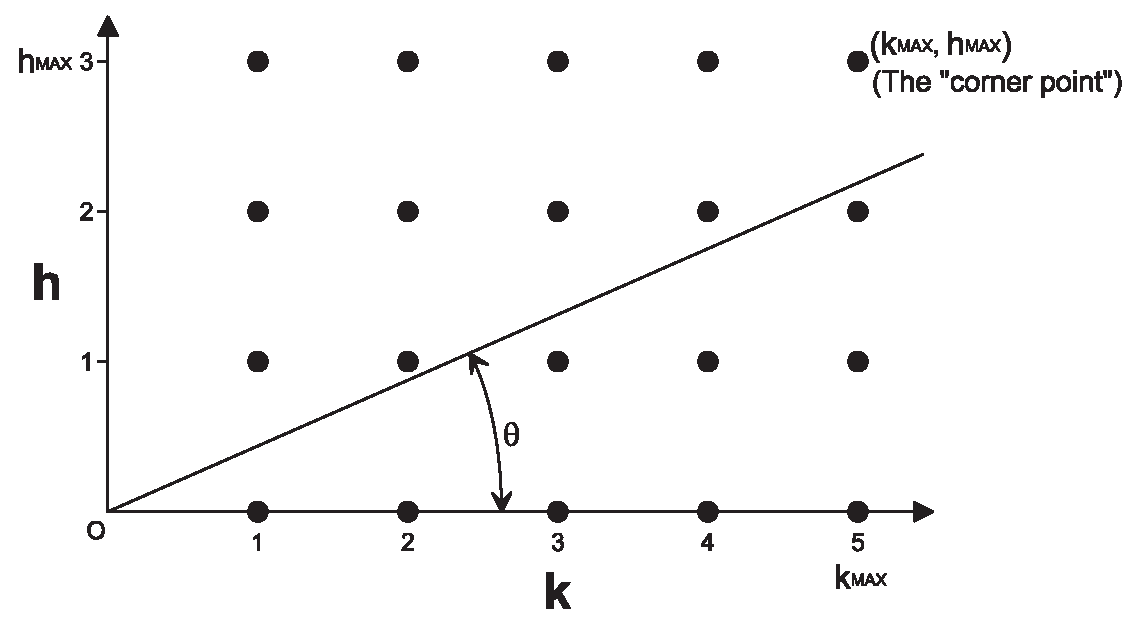
\includegraphics[width=4.6in]{c_rla1/farey01a.eps}
\caption{Graphical Interpretation Of Rational Numbers 
         $h/k$ That Can Be Formed With $h \leq h_{MAX}=3$, $k \leq k_{MAX}=5$}
\label{fig:crla1:slcr0:sfry0:00}
\end{figure}

From the graphical interpretation suggested by Fig. \ref{fig:crla1:slcr0:sfry0:00},
the following properties are intuitively clear.

\begin{itemize}
   \item The angle of a ray drawn from the origin to the point
         $(k,h)$ corresponding to the rational number $h/k$ is
         $\theta = tan^{-1} \; h/k$.

   \item Any integer lattice point on a line from 
         the origin drawn at the angle $\theta$
         has the value $h/k = tan \; \theta$.  All points corresponding
         to rational numbers with the same value will be on such a line,
         and thus form an equivalence class.

   \item A rational number $h/k$ is irreducible if and only if its corresponding
         point $(k,h)$ is ``directly'' visible from the origin with
         no intervening points.

   \item The Farey series of order $N$, $F_N$, can be 
         formed graphically by starting with the
         set of integer lattice points
         $(k,h): \; h \in \vworkintsetnonneg \wedge 1 \leq k \leq N$, 
         then sweeping
         a line extended from the origin, starting with 
         angle $\theta = 0$, through
         $0 \leq \theta < \pi{}/2$, and recording 
         in order each point directly visible from
         the origin.\footnote{Note that Fig. \ref{fig:crla1:slcr0:sfry0:00},
         because it illustrates the case when $h$ is constrained
         as well, does not show integer lattice points for
         $h > h_{MAX}$.  In principle, if the integer lattice shown
         in Fig. \ref{fig:crla1:slcr0:sfry0:00} were extended indefinitely
         ``upward'', every positive irreducible rational number with
         $k \leq k_{MAX} = 5$ could be found graphically.}
\end{itemize}

Fig. \ref{fig:crla1:slcr0:sfry0:01} illustrates the graphical construction method
of $F_5$.  Note that only integer lattice points which are directly
visible from the origin (with no intervening points) are selected.
(Fig. \ref{fig:crla1:slcr0:sfry0:01}, like Fig. \ref{fig:crla1:slcr0:sfry0:00},
shows the case of constrained $h$---the integer lattice should be
continued ``upward'' to construct the Farey series.)

\begin{figure}
\centering
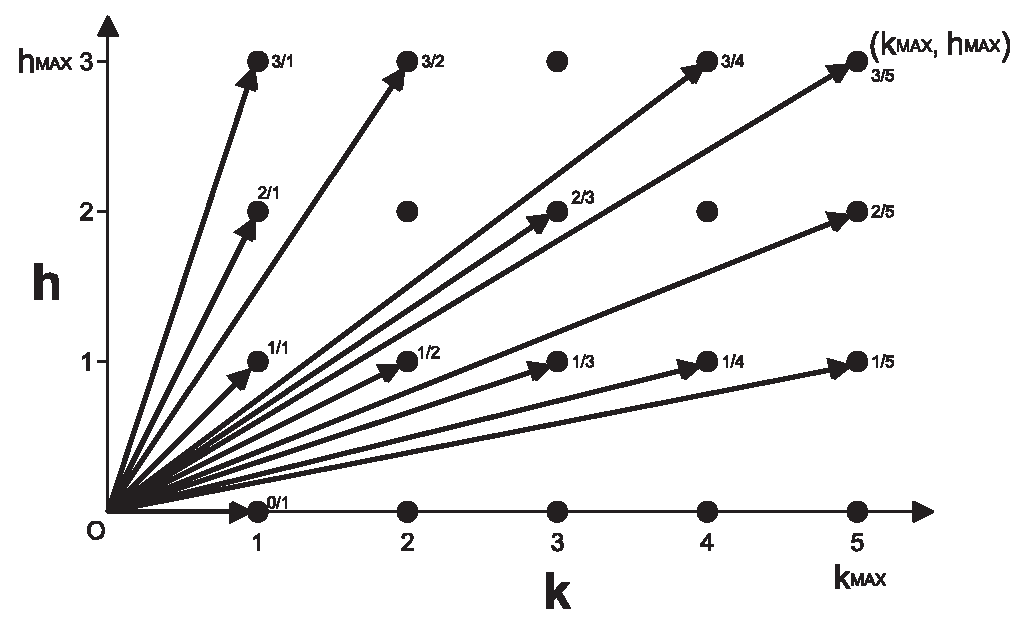
\includegraphics[width=4.6in]{c_rla1/farey01b.eps}
\caption{Graphical Interpretation Of Irreducible Rational Numbers 
         $h/k$ That Can Be Formed With $h \leq h_{MAX}=3$, $k \leq k_{MAX}=5$}
\label{fig:crla1:slcr0:sfry0:01}
\end{figure}

Note that Figures \ref{fig:crla1:slcr0:sfry0:00}
and \ref{fig:crla1:slcr0:sfry0:01} depict the case when
\emph{both} $h$ and $k$ are constrained (whereas the Farey series
constrains only $k$).

To give a compact notation, we denote the set of ascending irreducible
rational numbers that can be graphically formed
from Figures \ref{fig:crla1:slcr0:sfry0:00}
and \ref{fig:crla1:slcr0:sfry0:01} as  
$F_{k_{MAX}, h_{MAX}}$.  Using this notation, the graphical construction method
depicted in Figure \ref{fig:crla1:slcr0:sfry0:01} identifies $F_{5,3}$.

The ``corner point'' in Figures \ref{fig:crla1:slcr0:sfry0:00}
and \ref{fig:crla1:slcr0:sfry0:01} plays a special role:

\begin{itemize}
\item From 0/1 up through the corner point $h_{MAX}/k_{MAX}$,
      the terms are the terms of the Farey series of order
      $k_{MAX}$.
\item From $h_{MAX}/k_{MAX}$ up through $h_{MAX}/1$, the terms
      are the reverse-ordered reciprocals of the terms of the
      Farey series of order $h_{MAX}$.\footnote{This can be verified
      by transposing the $h$ and $k$ axes of the figures.}
\end{itemize}

As an example, $F_{5,3}$ identified graphically
is Figure \ref{fig:crla1:slcr0:sfry0:01} is

\begin{equation}
\label{eq:crla1:slcr0:sfry0:10}
F_5  = \left\{ {\frac{0}{1},\frac{1}{5},\frac{1}{4},
                \frac{1}{3},\frac{2}{5},\frac{1}{2},
                \frac{3}{5},\frac{2}{3},\frac{3}{4},
                \frac{1}{1},\frac{3}{2}, \frac{2}{1},
                \frac{3}{1} } \right\} .
\end{equation}

It can be seen by comparing (\ref{eq:crla1:slcr0:sfry0:10})
with (\ref{eq:crla1:slcr0:sfry0:eq0001c}) and 
(\ref{eq:crla1:slcr0:sfry0:eq0001e}) that the first seven terms of
(\ref{eq:crla1:slcr0:sfry0:10}) come from $F_5$ and the remaining
six terms are the reverse-ordered reciprocals of $F_3$ (although $F_3$
must be extended from Eq. \ref{eq:crla1:slcr0:sfry0:eq0001c}
into [1,2] to include 4/3 and 3/2).

The symmetry of Figures \ref{fig:crla1:slcr0:sfry0:00} and 
\ref{fig:crla1:slcr0:sfry0:01} with respect to the corner point
is important, because it means that finding best 
rational approximations for 
$r_I < h_{MAX}/k_{MAX}$ is the same problem as for 
$r_I > h_{MAX}/k_{MAX}$.  In the case of
$r_I < h_{MAX}/k_{MAX}$, the Farey series of order
$k_{MAX}$ is used, and in the case of
$r_I > h_{MAX}/k_{MAX}$ the Farey series of order
$h_{MAX}$ is used (but the reciprocals of the terms are
used, the order of the terms is reversed, and $1/r_I$ is used).  Thus, if we
know how to bracket $r_I < h_{MAX}/k_{MAX}$
in $F_{k_{MAX}}$, we can approach
the problem of $r_I > h_{MAX}/k_{MAX}$
through the inherent symmetry.


%%%%%%%%%%%%%%%%%%%%%%%%%%%%%%%%%%%%%%%%%%%%%%%%%%%%%%%%%%%%%%%%%%%%%%%%%%%%%%%
%%%%%%%%%%%%%%%%%%%%%%%%%%%%%%%%%%%%%%%%%%%%%%%%%%%%%%%%%%%%%%%%%%%%%%%%%%%%%%%
%%%%%%%%%%%%%%%%%%%%%%%%%%%%%%%%%%%%%%%%%%%%%%%%%%%%%%%%%%%%%%%%%%%%%%%%%%%%%%%

\subsection{The Continued Fraction Algorithm}

%Subsection Tag: cfr0
\label{crla1:slcr0:scfr0}

A \emph{finite simple continued fraction} is a fraction of the form

\begin{equation}
\label{eq:crla1:slcr0:scfr0:00}
a_0 + \cfrac{1}{a_1 + \cfrac{1}{a_2
    + \cfrac{1}{\;\;\;\;\;\;\;\;\;\;\;\;\;\;\ldots + \cfrac{1}{a_n}}}}
    =
    [a_0; a_1, a_2, \ldots , a_n] ,
\end{equation}

\noindent{}where $a_0 \in \vworkintsetnonneg$ and 
$a_i \in \vworkintsetpos$, $i > 0$.  Each integer
$a_i$ is called an \index{continued fraction!element}\emph{element} or
\index{continued fraction!partial quotient}\emph{partial quotient} 
of the continued fraction.
To ensure a unique representation, we require, except in the case of
the continued fraction representation of an integer,
that the final element $a_n$ not be equal
to 1.

Continued fractions are quite unwieldly to write and typeset,
and so a continued fraction in the form of (\ref{eq:crla1:slcr0:scfr0:00})
is written as $[a_0; a_1, a_2, \ldots , a_n]$.  Note that the
separator between $a_0$ and $a_1$ is a semicolon (`;'), and that all other
separators are commas (`,').  In some works, commas are used exclusively; and in
other works, the first element is $a_1$ rather than $a_0$.  Throughout this
work, the notational conventions illustrated in (\ref{eq:crla1:slcr0:scfr0:00}) are
followed.

Continued fractions can be either finite or infinite.

A finite continued fraction consists of a finite number of elements
$[a_0; a_1, a_2, \ldots , a_n]$.  It can be proved that 
every rational number corresponds to a unique
finite continued fraction\footnote{So long as the $a_n \neq 1$ convention
described earlier is followed.}, and that 
every finite continued fraction corresponds to a rational number. 

An infinite continued fraction consists of an infinite number
of elements $[a_0; a_1, a_2, \ldots]$.  Because every rational number
corresponds to a finite continued fraction, all irrational numbers have
infinite continued fraction representations.

In engineering work (and due to the general prevalence of computers
and calculators), any $r_I$ to be approximated has a known approximate
numerical value.  Even quantities that are known to be irrational (such
as $\pi$ or $\sqrt{2}$) have a numerical value known to a large number
of significant digits.  For this reason, only the numerical procedure for
obtaining the continued fraction representation of a rational number is
presented here (the symbolic procedure is not discussed).  Numerical values
are always rational (for example, 3.1415 is 31,415/10,000).

\index{continued fraction!convergent}
The \emph{kth order convergent} of a continued fraction
$[a_0; a_1, \ldots{}, a_n]$ is the irreducible rational number
corresponding to $[a_0; a_1, \ldots{}, a_k]$, $k \leq n$.
In other words, the $k$th order convergent is the irreducible rational number
corresponding to the first $k+1$ partial quotients of a 
continued fraction.\footnote{``$k+1$'' because the notational
numbering
for partial quotients starts at 0 rather than 1.} 

An $n$th order continued fraction $[a_0; a_1, \ldots{}, a_n]$
has $n+1$ convergents, $[a_0]$, 
$[a_0; a_1]$, \ldots{}, and $[a_0; a_1, \ldots{}, a_n]$.
We denote the $k$th order convergent as $s_k$, with numerator
$p_k$ and denominator $q_k$.

Without proof, we present the following algorithm, Algorithm 
\ref{alg:crla1:slcr0:scfr0:akgenalg}, for
determining the continued fraction representation (i.e. the partial
quotients) as well as the convergents of a non-negative
rational number $a/b$.

\begin{vworkalgorithmstatementpar}{Continued Fraction Representation and
                                   Convergents of 
                                   A Rational Number \mbox{\boldmath $a/b$}}
\label{alg:crla1:slcr0:scfr0:akgenalg}
\begin{alglvl0}
\item $k:=-1$.
\item $divisor_{-1} := a$.
\item $remainder_{-1} := b$.

\item Repeat

\begin{alglvl1}
\item $k := k + 1$.
\item $dividend_k := divisor_{k-1}$.
\item $divisor_k  := remainder_{k-1}$.
\item $a_k :=  dividend_k \; div \; divisor_k$.
\item $remainder_k := dividend_k \; mod \; divisor_k$.
\item If $k=0$, $p_0 = a_0$; else if $k=1$, $p_1 = a_0 a_1 + 1$; 
      else $p_i = a_i p_{i-1} + p_{i-2}$.
\item If $k=0$, $q_0 = 1$; else if $k=1$, $q_1 = a_1$; 
      else $q_i = a_i q_{i-1} + q_{i-2}$.
\end{alglvl1}

\item Until ($remainder_k = 0$).
\end{alglvl0}
\textbf{\emph{Note:}} The final $s_k = p_k / q_k$ is the irreducible
form of $a/b$.  For brevity, this is not proved here.
\end{vworkalgorithmstatementpar}
%\vworkalgorithmfooter{}
\begin{vworkexamplestatement}
\label{ex:crla1:slcr0:scfr0:01}
Find the continued fraction partial quotients and convergents of 
$67/29$.
\end{vworkexamplestatement}
\begin{vworkexampleparsection}{Solution} Table 
\ref{tbl:crla1:slcr0:scfr0:01} shows the application of 
Algorithm \ref{alg:crla1:slcr0:scfr0:akgenalg} to find the
continued fraction partial quotients and convergents of $67/29$.  From
Table \ref{tbl:crla1:slcr0:scfr0:01}, the continued fraction
representation of $67/29$ is $[2;3,4,2]$.

\begin{table}
\caption{Continued Fraction Partial Quotients and Convergents of $67/29$ (Example \ref{ex:crla1:slcr0:scfr0:01})}
\label{tbl:crla1:slcr0:scfr0:01}
\begin{center}
\begin{tabular}{|c|c|c|c|c|c|c|}
\hline
\small{Index} & \small{$dividend_k$}  & \small{$divisor_k$} & \small{$a_k$}   & \small{$remainder_k$} & \small{$p_k$} & \small{$q_k$} \\
\small{($k$)} &                       &                     &                 &                       &               &               \\
\hline
\hline
\small{-1}    & \small{N/A}           & \small{67}          & \small{N/A}     & \small{29}            & \small{N/A}   & \small{N/A}   \\
\hline
\small{0}     & \small{67}            & \small{29}          & \small{2}       & \small{9}             & \small{2}     & \small{1}     \\
\hline
\small{1}     & \small{29}            & \small{9}           & \small{3}       & \small{2}             & \small{7}     & \small{3}     \\
\hline
\small{2}     & \small{9}             & \small{2}           & \small{4}       & \small{1}             & \small{30}    & \small{13}    \\
\hline
\small{3}     & \small{2}             & \small{1}           & \small{2}       & \small{0}             & \small{67}    & \small{29}    \\
\hline
\end{tabular}
\end{center}
\end{table}
\end{vworkexampleparsection}
\vworkexamplefooter{}

Finally, we present without proof a theorem that indicates how to bracket
a rational number $a/b$ that is not in $F_{k_{MAX}}$ with its two neighbors
in $F_{k_{MAX}}$.

\begin{vworktheoremstatementpar}{Enclosing Neighbors Of \mbox{\boldmath $x \notin F_N$} 
                                 In \mbox{\boldmath $F_N$}}
\label{thm:crla1:slcr0:scfr0:cfenclosingneighbors}
For a non-negative rational
number $a/b$\footnote{It is not required that $a/b$ be irreducible in
order to apply this theorem.
For brevity, many properties of convergents were omitted; it is provable that 
the convergents formed by Algorithm \ref{alg:crla1:slcr0:scfr0:akgenalg}
will be identical for $a/b$ and $ia/ib$.} not in
$F_N$ which has a
continued fraction representation
$[a_0;a_1,a_2,\ldots{} ,a_n]$, the
highest-order convergent $s_k = p_k/q_k$ with $q_k \leq N$ is one
neighbor\footnote{By neighbors in $F_N$ we mean the rational numbers
in $F_N$ immediately to the left and immediately to the right
of $a/b$.}
to $a/b$ in $F_N$, and the other neighbor in
$F_N$ is\footnote{Theorem \ref{thm:crla1:slcr0:scfr0:cfenclosingneighbors}
is a somewhat stronger statement about best approximations
than Khinchin makes in \cite{bibref:b:KhinchinClassic}, Theorem 15.
We were not able to locate
this theorem or a proof in print,
but this theorem is understood within the number theory community.
It appears on the Web
page of David Eppstein \cite{bibref:i:davideppstein} in the form of a
`C'-language computer program,
\texttt{http://www.ics.uci.edu/\~{}{}eppstein/numth/frap.c}.
Although
Dr. Eppstein phrases the solution in terms of modifying
a partial quotient, his approach is equivalent to
(\ref{eq:crla1:slcr0:scfr0:thm:cfenclosingneighbors:01}).}

\begin{equation}
\label{eq:crla1:slcr0:scfr0:thm:cfenclosingneighbors:01}
\frac{{\displaystyle{\left\lfloor {\frac{{N - q_{k - 1} }}{{q_k }}} \right\rfloor}
 p_k  + p_{k - 1} }}{{\displaystyle{\left\lfloor {\frac{{N - q_{k - 1} }}{{q_k }}}
 \right\rfloor} q_k  + q_{k - 1} }}.
\end{equation}
\end{vworktheoremstatementpar}
\begin{vworktheoremproof}
Omitted, as it relies on material not presented for brevity.
\end{vworktheoremproof}
\vworktheoremfooter{}

Theorem \ref{thm:crla1:slcr0:scfr0:cfenclosingneighbors}
can also be applied to find the Farey neighbors of an $a/b$ already
in $F_{k_{MAX}}$.  If Algorithm \ref{alg:crla1:slcr0:scfr0:akgenalg}
is applied to $a/b$, (\ref{eq:crla1:slcr0:scfr0:thm:cfenclosingneighbors:01})
will provide one Farey neighbor, and 
(\ref{eq:crla1:slcr0:sfry0:thm:01:eq01}) through
(\ref{eq:crla1:slcr0:sfry0:thm:01:eq04}) can be used to provide the other
Farey neighbor.  (Again, for brevity, the mathematical basis for this
is not presented.)

Many constants $r_I$ to be approximated are engineering constants based
on measurements or arbitrary conventions, and so are known or accepted to
only a finite number of significant digits.  Such constants are always
rational, and 
Algorithm \ref{alg:crla1:slcr0:scfr0:akgenalg}
and
Theorem \ref{thm:crla1:slcr0:scfr0:cfenclosingneighbors}
can be applied with no special consideration.

Some constants, however, are irrational.  The question naturally arises
of how to be sure that one is using enough decimal digits
in applying 
Algorithm \ref{alg:crla1:slcr0:scfr0:akgenalg}
and
Theorem \ref{thm:crla1:slcr0:scfr0:cfenclosingneighbors}.
The easiest approach to apply in practice\footnote{\emph{In practice}
because some theoretical results may be possible as far as how
many significant digits are always adequate or as far as other
criteria, but the approach taken here is the easiest practical one.}
is to confine the quantity of interest by an inequality and to be
sure that the results are the same at both boundaries
of the inequality.

For example, $\pi$ is a transcendental constant, so has a non-terminating
decimal representation.  $\pi$ to several digits (truncated at the
end) is 3.1415926535.  It follows that

\begin{equation}
\label{eq:crla1:slcr0:scfr0:30}
3.1415926535 < \pi < 3.1415926536
\end{equation}  

For compact notation, we denote the left limit as $r_{LEFT}$ and the
right limit by $r_{RIGHT}$.  We also make the observation that in some
applications, the interval is closed rather than open.\footnote{This depends
on how much is known about $r_I$---for example, we know that $\pi$ is irrational and
can't be equal to any rational number, but we
may not know this about other $r_I$ of interest.}  In the more
general case, $r_I$ is confined by:

\begin{equation}
\label{eq:crla1:slcr0:scfr0:30b}
r_{LEFT} \leq r_I < r_{RIGHT} .
\end{equation}  

With the the $r_I$ of interest confined as suggested in 
(\ref{eq:crla1:slcr0:scfr0:30b}), there are two easy approaches
to decide if the Farey neighbors of $r_I$ can be determined with
the information available.

\begin{enumerate}
\item \emph{Easier:} Locate the Farey neighbors $h_L/k_L$ and $h_R/k_R$ of
      $r_{LEFT}$, then numerically determine whether 
      $h_L/k_L \leq r_{RIGHT} \leq h_R/k_R$.
\item \emph{Harder:} Determine whether $r_{LEFT}$ and $r_{RIGHT}$ have the
      same convergents up through $p_k/q_k$ with $q_k \leq N$.  If so,
      $r_{LEFT}$ and $r_{RIGHT}$ have the same Farey neighbors.
\end{enumerate}

\noindent{}If 
Algorithm \ref{alg:crla1:slcr0:scfr0:akgenalg}
and
Theorem \ref{thm:crla1:slcr0:scfr0:cfenclosingneighbors} are
applied with 31415926535/10000000000 and 31415926536/10000000000 
separately and yield the same rational numbers $h_L/k_L$ and $h_R/k_R$ as 
left and right neighbors, then

\begin{equation}
\label{eq:crla1:slcr0:scfr0:31}
\frac{h_L}{k_L} < 3.1415926535 < \pi < 3.1415926536 < \frac{h_R}{k_R}
\end{equation}  

\noindent{}and it is thus confirmed that $h_L/k_L$ and $h_R/k_R$ are the left
and right neighbors of $\pi$ in the Farey series of interest.

Several examples follow which illustrate the technique and various special
cases.

\begin{vworkexamplestatement}
\label{ex:crla1:slcr0:scfr0:10}
Find the best rational approximation to $1/e$ in $F_{65535}$.
\end{vworkexamplestatement}
\begin{vworkexampleparsection}{Solution} Note that $e$ is irrational, implying
that $1/e$ is also irrational, thus a bounding technique might best be used
to ensure finding the correct Farey neighbors.  Using an ordinary scientific pocket
calculator, the displayed value of $e^{-1}$ is approximately 0.367879441171.
Allowing for some possible imprecision in the last digit\footnote{The guess at 
how accurate a calculator is likely to be is subjective.}, it is fairly safe to assume that

\begin{equation}
\label{eq:ex:crla1:slcr0:scfr0:10:01}
\frac{367879441170}{1000000000000} < \frac{1}{e} < \frac{367879441172}{1000000000000} .
\end{equation}

Table \ref{tbl:crla1:slcr0:scfr0:10a} shows the application of 
Algorithm \ref{alg:crla1:slcr0:scfr0:akgenalg} to find the
continued fraction partial quotients of the left inequality
limit, and Table Table \ref{tbl:crla1:slcr0:scfr0:10b} shows the
calculation of the convergents.  (The tables are separated due to typesetting
limitations---the partial quotients and convergents would normally be tabulated
together.)

\begin{table}
\caption{Continued Fraction Partial Quotients of $367,879,441,170/1,000,000,000,000$ (Example \ref{ex:crla1:slcr0:scfr0:10})}
\label{tbl:crla1:slcr0:scfr0:10a}
\begin{center}
\begin{tabular}{|c|c|c|c|c|}
\hline
\small{Index} & \small{$dividend_k$}      & \small{$divisor_k$}       & \small{$a_k$}   & \small{$remainder_k$}     \\
\small{($k$)} &                           &                           &                 &                           \\
\hline
\hline
\small{-1}    & \small{N/A}               & \small{367,879,441,170}   & \small{N/A}     & \small{1,000,000,000,000} \\
\hline
\small{0}     & \small{367,879,441,170}   & \small{1,000,000,000,000} & \small{0}       & \small{367,879,441,170}   \\
\hline
\small{1}     & \small{1,000,000,000,000} & \small{367,879,441,170}   & \small{2}       & \small{264,241,117,660}   \\
\hline
\small{2}     & \small{367,879,441,170}   & \small{264,241,117,660}   & \small{1}       & \small{103,638,323,510}   \\
\hline
\small{3}     & \small{264,241,117,660}   & \small{103,638,323,510}   & \small{2}       & \small{56,964,470,640}    \\
\hline
\small{4}     & \small{103,638,323,510}   & \small{56,964,470,640}    & \small{1}       & \small{46,673,852,870}    \\
\hline
\small{5}     & \small{56,964,470,640}    & \small{46,673,852,870}    & \small{1}       & \small{10,290,617,770}    \\
\hline
\small{6}     & \small{46,673,852,870}    & \small{10,290,617,770}    & \small{4}       & \small{5,511,381,790}     \\
\hline
\small{7}     & \small{10,290,617,770}    & \small{5,511,381,790}     & \small{1}       & \small{4,779,235,980}     \\
\hline
\small{8}     & \small{5,511,381,790}     & \small{4,779,235,980}     & \small{1}       & \small{732,145,810}       \\
\hline
\small{9}     & \small{4,779,235,980}     & \small{732,145,810}       & \small{6}       & \small{386,361,120}       \\
\hline
\small{10}    & \small{732,145,810}       & \small{386,361,120}       & \small{1}       & \small{345,784,690}       \\
\hline
\small{11}    & \small{386,361,120}       & \small{345,784,690}       & \small{1}       & \small{40,576,430}        \\
\hline
\small{12}    & \small{345,784,690}       & \small{40,576,430}        & \small{8}       & \small{21,173,250}        \\
\hline
\small{13}    & \small{40,576,430}       & \small{21,173,250}         & \small{1}       & \small{19,403,180}        \\
\hline
\small{14}    & \small{21,173,250}       & \small{19,403,180}         & \small{1}       & \small{1,770,070}         \\
\hline
\small{15}    & \small{19,403,180}       & \small{1,770,070}          & \small{10}      & \small{1,702,480}         \\
\hline
\small{16}    & \small{1,770,070}        & \small{1,702,480}          & \small{1}       & \small{67,590}            \\
\hline
\small{17}    & \small{1,702,480}        & \small{67,590}             & \small{25}      & \small{12,730}            \\
\hline
\small{18}    & \small{67,590}           & \small{12,730}             & \small{5}       & \small{3,940}             \\
\hline
\small{19}    & \small{12,730}           & \small{3,940}              & \small{3}       & \small{910}               \\
\hline
\small{20}    & \small{3,940}            & \small{910}                & \small{4}       & \small{300}               \\
\hline
\small{21}    & \small{910}              & \small{300}                & \small{3}       & \small{10}                \\
\hline
\small{22}    & \small{300}              & \small{10}                 & \small{30}      & \small{0}                 \\
\hline
\end{tabular}
\end{center}
\end{table}

\begin{table}
\caption{Continued Fraction Convergents of $367,879,441,170/1,000,000,000,000$ (Example \ref{ex:crla1:slcr0:scfr0:10})}
\label{tbl:crla1:slcr0:scfr0:10b}
\begin{center}
\begin{tabular}{|c|c|c|c|}
\hline
\small{Index} & \small{$a_k$} & \small{$p_k$}           & \small{$q_k$}            \\
\small{($k$)} &               &                         &                          \\
\hline
\hline
\small{-1}    & \small{N/A}   & \small{N/A}             & \small{N/A}              \\
\hline
\small{0}     & \small{0}     & \small{0}               & \small{1}                \\
\hline
\small{1}     & \small{2}     & \small{1}               & \small{2}                \\
\hline
\small{2}     & \small{1}     & \small{1}               & \small{3}                \\
\hline
\small{3}     & \small{2}     & \small{3}               & \small{8}                \\
\hline
\small{4}     & \small{1}     & \small{4}               & \small{11}               \\
\hline
\small{5}     & \small{1}     & \small{7}               & \small{19}               \\
\hline
\small{6}     & \small{4}     & \small{32}              & \small{87}               \\
\hline
\small{7}     & \small{1}     & \small{39}              & \small{106}              \\
\hline
\small{8}     & \small{1}     & \small{71}              & \small{193}              \\
\hline
\small{9}     & \small{6}     & \small{465}             & \small{1,264}            \\
\hline
\small{10}    & \small{1}     & \small{536}             & \small{1,457}            \\
\hline
\small{11}    & \small{1}     & \small{1,001}           & \small{2,721}            \\
\hline
\small{12}    & \small{8}     & \small{8,544}           & \small{23,225}           \\
\hline
\small{13}    & \small{1}     & \small{9,545}           & \small{25,946}           \\
\hline
\small{14}    & \small{1}     & \small{18,089}          & \small{49,171}          \\
\hline
\small{15}    & \small{10}    & \small{190,435}         & \small{517,656}         \\
\hline
\small{16}    & \small{1}     & \small{208,524}         & \small{566,827}          \\
\hline
\small{17}    & \small{25}    & \small{5,403,535}       & \small{14,688,331}       \\
\hline
\small{18}    & \small{5}     & \small{27,226,199}      & \small{74,008,482}       \\
\hline
\small{19}    & \small{3}     & \small{87,082,132}      & \small{236,713,777}      \\
\hline
\small{20}    & \small{4}     & \small{375,554,727}     & \small{1,020,863,590}    \\
\hline
\small{21}    & \small{3}     & \small{1,213,746,313}   & \small{3,299,304,547}    \\
\hline
\small{22}    & \small{30}    & \small{36,787,944,117}  & \small{100,000,000,000}  \\
\hline
\end{tabular}
\end{center}
\end{table}

Note that since we are finding best rational approximations
in $F_{65535}$, Theorem \ref{thm:crla1:slcr0:scfr0:cfenclosingneighbors}
requires only that we carry the tabular procedure of 
Algorithm \ref{alg:crla1:slcr0:scfr0:akgenalg} out until
$q_k \geq 65535$ ($k=15$ in this example).

By
Theorem \ref{thm:crla1:slcr0:scfr0:cfenclosingneighbors}
and
Table \ref{tbl:crla1:slcr0:scfr0:10b}, one Farey neighbor
to the left inequality limit is $p_{14}/q_{14} = 18,089/49,171$.
The other Farey neighbor is given by 
(\ref{eq:crla1:slcr0:scfr0:thm:cfenclosingneighbors:01}), with the calculation
detailed below.

\begin{equation}
\label{eq:ex:crla1:slcr0:scfr0:10:50a}
\frac{{\displaystyle{\left\lfloor {\frac{{N - q_{k - 1} }}{{q_k }}} \right\rfloor}
 p_k  + p_{k - 1} }}{{\displaystyle{\left\lfloor {\frac{{N - q_{k - 1} }}{{q_k }}}
 \right\rfloor} q_k  + q_{k - 1} }}.
\end{equation}

\begin{equation}
\label{eq:ex:crla1:slcr0:scfr0:10:50b}
= \frac{{\displaystyle{\left\lfloor {\frac{{65535 - q_{13} }}{{q_{14} }}} \right\rfloor}
 p_{14}  + p_{13} }}{{\displaystyle{\left\lfloor {\frac{{65535 - q_{13} }}{{q_{14} }}}
 \right\rfloor} q_{14}  + q_{13} }}.
\end{equation}

\begin{equation}
\label{eq:ex:crla1:slcr0:scfr0:10:50c}
= \frac{{\displaystyle{\left\lfloor {\frac{{65535 - 25946 }}{{49171 }}} \right\rfloor}
 18089  + 9545 }}{{\displaystyle{\left\lfloor {\frac{{65535 - 25946 }}{{49171 }}}
 \right\rfloor} 49171  + 25946 }}.
\end{equation}

\begin{equation}
\label{eq:ex:crla1:slcr0:scfr0:10:50d}
= \frac{9545}{25946}
\end{equation}

It can be verified by cross-multiplication that $9545/25946 > 18089/49171$, therefore

\begin{equation}
\label{eq:ex:crla1:slcr0:scfr0:10:50e}
\frac{18089}{49171} < 0.367879441170 < \frac{9545}{25946} .
\end{equation}

A similar tabulation procedure carried out with 
the right inequality limit (0.367879441172), not reproduced here for brevity,
verifies that it has the same convergents up through $s_{15}$ as the left
inequality limit.  Therefore it has the same Farey neighbors in $F_{65535}$
as the left limit, and it is established that

\begin{equation}
\label{eq:ex:crla1:slcr0:scfr0:10:50f}
\frac{18089}{49171} < 0.367879441170 < \frac{1}{e} < 0.367879441172 < \frac{9545}{25946} .
\end{equation}

It can be verified numerically that 18089/49171 and 9545/25946 are both \emph{very}
close approximations to $1/e$ (with differences on the order of a couple parts per
\emph{billion}).
\end{vworkexampleparsection}
%\vworkexamplefooter{}

\begin{vworkexamplestatement}
\label{ex:crla1:slcr0:scfr0:11}
Find the enclosing neighbors to $8/43$ in $F_{65535}$.
\end{vworkexamplestatement}
\begin{vworkexampleparsection}{Solution} As hinted earlier,
since $8/43 \in F_{65535}$, we can simply treat 8/43 as a number very close to 8/43
so that the convergent after $s_k = 8/43$ has a larger denominator than 65535 (the details
of why and how this works are omitted for brevity).

\begin{table}
\caption{Continued Fraction Partial Quotients and Convergents of $8/43$ (Example \ref{ex:crla1:slcr0:scfr0:11})}
\label{tbl:crla1:slcr0:scfr0:11a}
\begin{center}
\begin{tabular}{|c|c|c|c|c|c|c|}
\hline
\small{Index} & \small{$dividend_k$} & \small{$divisor_k$} & \small{$a_k$} & \small{$remainder_k$} & \small{$p_k$} & \small{$q_k$} \\
\small{($k$)} &                      &                     &               &                       &               &               \\
\hline
\hline
\small{-1}    & \small{N/A}          & \small{8}           & \small{N/A}   & \small{43}            & \small{N/A}   & \small{N/A}   \\
\hline
\small{0}     & \small{8}            & \small{43}          & \small{0}     & \small{8}             & \small{0}     & \small{1}     \\
\hline
\small{1}     & \small{43}           & \small{8}           & \small{5}     & \small{3}             & \small{1}     & \small{5}     \\
\hline
\small{2}     & \small{8}            & \small{3}           & \small{2}     & \small{2}             & \small{2}     & \small{11}    \\
\hline
\small{3}     & \small{3}            & \small{2}           & \small{1}     & \small{1}             & \small{3}     & \small{16}    \\
\hline
\small{4}     & \small{2}            & \small{1}           & \small{2}     & \small{0}             & \small{8}     & \small{43}    \\
\hline
\end{tabular}
\end{center}
\end{table}

Table \ref{tbl:crla1:slcr0:scfr0:11a} shows the
application of 
Algorithm \ref{alg:crla1:slcr0:scfr0:akgenalg}
to determine the partial quotients and convergents of 8/43.

(\ref{eq:crla1:slcr0:scfr0:thm:cfenclosingneighbors:01}) can then be applied
to find a Farey neighbor of 8/43, with the calculation
detailed below.\footnote{Whether the left or right Farey neighbor is found depends on
whether the final convergent has $k$ even or $k$ odd.  The explanation is beyond the scope here.}

\begin{equation}
\label{eq:ex:crla1:slcr0:scfr0:11:50a}
\frac{{\displaystyle{\left\lfloor {\frac{{N - q_{k - 1} }}{{q_k }}} \right\rfloor}
 p_k  + p_{k - 1} }}{{\displaystyle{\left\lfloor {\frac{{N - q_{k - 1} }}{{q_k }}}
 \right\rfloor} q_k  + q_{k - 1} }}.
\end{equation}

\begin{equation}
\label{eq:ex:crla1:slcr0:scfr0:11:50b}
= \frac{{\displaystyle{\left\lfloor {\frac{{65535 - q_{3} }}{{q_{4} }}} \right\rfloor}
 p_{4}  + p_{3} }}{{\displaystyle{\left\lfloor {\frac{{65535 - q_{3} }}{{q_{4} }}}
 \right\rfloor} q_{4}  + q_{3} }}.
\end{equation}

\begin{equation}
\label{eq:ex:crla1:slcr0:scfr0:11:50c}
= \frac{{\displaystyle{\left\lfloor {\frac{{65535 - 16 }}{{43 }}} \right\rfloor}
 8  + 3 }}{{\displaystyle{\left\lfloor {\frac{{65535 - 16 }}{{43 }}}
 \right\rfloor} 43  + 16 }}.
\end{equation}

\begin{equation}
\label{eq:ex:crla1:slcr0:scfr0:11:50d}
= \frac{12187}{65505}
\end{equation}

It can be verified by cross-multiplication that (\ref{eq:ex:crla1:slcr0:scfr0:11:50d})
is the right Farey neighbor of 8/43.  As two consecutive
terms in $F_{65535}$ are now known, (\ref{eq:crla1:slcr0:sfry0:thm:01:eq03})
and (\ref{eq:crla1:slcr0:sfry0:thm:01:eq04}) can be applied to find the left Farey
neighbor, as shown below.

\begin{equation}
\label{eq:ex:crla1:slcr0:scfr0:11:51}
h_j  = \left\lfloor {\frac{{k_{j + 2}  + N}}{{k_{j + 1} }}} 
\right\rfloor h_{j + 1}  - h_{j + 2}
\end{equation}

\begin{equation}
\label{eq:ex:crla1:slcr0:scfr0:11:52}
= \left\lfloor {\frac{{65505  + 65535}}{{43 }}} 
\right\rfloor 8  - 12187 = 12189
\end{equation}

\begin{equation}
\label{eq:ex:crla1:slcr0:scfr0:11:55}
k_j  = \left\lfloor {\frac{{k_{j + 2}  + N}}{{k_{j + 1} }}} 
\right\rfloor k_{j + 1}  - k_{j + 2}
\end{equation}

\begin{equation}
\label{eq:ex:crla1:slcr0:scfr0:11:56}
= \left\lfloor {\frac{{65505  + 65535}}{{43 }}} 
\right\rfloor 43  - 65505 = 65516
\end{equation}

Thus, 12189/65516 is the left neighbor to 8/43 in $F_{65535}$.
\end{vworkexampleparsection}
%\vworkexamplefooter{}

\begin{vworkexamplestatement}
\label{ex:crla1:slcr0:scfr0:12}
Create assembly-language code to form an approximation 
to multiplication by $\pi$ that 
can be implemented using a \texttt{MUL} instruction followed by
a \texttt{DIV} instruction on the Freescale CPU08 core.  Assume that:
\begin{itemize}
\item The input is an 8-bit unsigned integer, passed in the accumulator.
\item The output is an 8-bit unsigned integer, returned in the accumulator.
\item The code is ``in-line'' (i.e. not a subroutine), and the code is free to modify
      any processor registers or flags.
\item Input data that is too large should cause the output to be clipped at 255 (the
      maximum value for an unsigned byte).
\end{itemize}
\end{vworkexamplestatement}
\begin{vworkexampleparsection}{Solution} $\pi$ is transcendental, and based
on the first several digits, can be bounded by

\begin{equation}
\label{eq:ex:crla1:slcr0:scfr0:12:01}
3.1415926535 < \pi < 3.1415926536 .
\end{equation}  

We first note that, due to the charactertistics of the CPU08, 
$h_{MAX} = 255$ and $k_{MAX} = 255$.  We are thus operating in
$F_{255, 255}$, with a corner point of $h/k = 255/255 = 1$.
$\pi > 1$, so we are operating along the top side of Figures
\ref{fig:crla1:slcr0:sfry0:00} and \ref{fig:crla1:slcr0:sfry0:01}
(pages \pageref{fig:crla1:slcr0:sfry0:00} and \pageref{fig:crla1:slcr0:sfry0:01}).
In this region above the corner point, the numerator rather than the denominator
is constrained.

As discussed earlier, to obtain best rational approximations above the corner point,
we may transpose the problem to that of obtaining best rational approximations
to $1/\pi$ in $F_{h_{MAX}}$ (rather than $F_{k_{MAX}}$---it is coincidental in this
case that $h_{MAX} = k_{MAX}$).

Algorithm \ref{alg:crla1:slcr0:scfr0:akgenalg} requires only a rational number as a starting
point, so it is most expedient to invert the terms of 
(\ref{eq:ex:crla1:slcr0:scfr0:12:01}) to yield

\begin{equation}
\label{eq:ex:crla1:slcr0:scfr0:12:02}
\frac{10000000000}{31415926536} 
< 
\frac{1}{\pi} 
< 
\frac{10000000000}{31415926535} .
\end{equation}

\begin{table}
\caption{Continued Fraction Partial Quotients and Convergents of $10000000000/31415926536$ (Example \ref{ex:crla1:slcr0:scfr0:12})}
\label{tbl:ex:crla1:slcr0:scfr0:12a}
\begin{center}
\begin{tabular}{|c|c|c|c|c|c|c|}
\hline
\small{$k$} & \small{$dividend_k$}  & \small{$divisor_k$}   & \small{$a_k$} & \small{$remainder_k$}    & \small{$p_k$}            & \small{$q_k$}            \\
\hline
\hline
\small{-1}   & \small{N/A}            & \small{10,000,000,000} & \small{N/A}    & \small{31,415,926,536}    & \small{N/A}               & \small{N/A}               \\
\hline
\small{0}    & \small{10,000,000,000} & \small{31,415,926,536} & \small{0}      & \small{10,000,000,000}    & \small{0}                 & \small{1}                 \\
\hline
\small{1}    & \small{31,415,926,536} & \small{10,000,000,000} & \small{3}      & \small{1,415,926,536}     & \small{1}                 & \small{3}                 \\
\hline
\small{2}    & \small{10,000,000,000} & \small{1,415,926,536}  & \small{7}      & \small{88,514,248}        & \small{7}                 & \small{22}                \\
\hline
\small{3}    & \small{1,415,926,536}  & \small{88,514,248}     & \small{15}     & \small{88,212,816}        & \small{106}               & \small{333}               \\
\hline
\multicolumn{7}{|c|}{\small{It isn't necessary to carry Algorithm \ref{alg:crla1:slcr0:scfr0:akgenalg}}}  \\ 
\multicolumn{7}{|c|}{\small{any further, as it has been established that $s_2 = 7/22$ is the last}}       \\
\multicolumn{7}{|c|}{\small{convergent with $q_k \leq 255$.}}                                             \\
\hline
\end{tabular}
\end{center}
\end{table}

Table \ref{tbl:ex:crla1:slcr0:scfr0:12a} shows the application of 
Algorithm \ref{alg:crla1:slcr0:scfr0:akgenalg} to obtain the partial
quotients and convergents of $10000000000/31415926536$.  Note that it is not
necessary to carry out the algorithm any further than establishing the
highest-order convergent with $q_k \leq h_{MAX} = 255$.

By Theorem \ref{thm:crla1:slcr0:scfr0:cfenclosingneighbors} 7/22 is either
the left or right Farey neighbor to 10000000000/31415926536.  Numerically,
it can be verified that 7/22 is the left Farey neighbor.

The right Farey neighbor is given by 
(\ref{eq:crla1:slcr0:scfr0:thm:cfenclosingneighbors:01}), with the calculation
detailed below.

\begin{equation}
\label{eq:ex:crla1:slcr0:scfr0:12:10a}
\frac{{\displaystyle{\left\lfloor {\frac{{N - q_{k - 1} }}{{q_k }}} \right\rfloor}
 p_k  + p_{k - 1} }}{{\displaystyle{\left\lfloor {\frac{{N - q_{k - 1} }}{{q_k }}}
 \right\rfloor} q_k  + q_{k - 1} }}
\end{equation}

\begin{equation}
\label{eq:ex:crla1:slcr0:scfr0:12:10b}
= \frac{{\displaystyle{\left\lfloor {\frac{{255 - q_{1} }}{{q_{2} }}} \right\rfloor}
 p_{2}  + p_{1} }}{{\displaystyle{\left\lfloor {\frac{{255 - q_{1} }}{{q_{2} }}}
 \right\rfloor} q_{2}  + q_{1} }}
\end{equation}

\begin{equation}
\label{eq:ex:crla1:slcr0:scfr0:12:10c}
= \frac{{\displaystyle{\left\lfloor {\frac{{255 - 3 }}{{22 }}} \right\rfloor}
 7  + 1 }}{{\displaystyle{\left\lfloor {\frac{{255 - 3 }}{{22 }}}
 \right\rfloor} 22  + 3 }}
\end{equation}

\begin{equation}
\label{eq:ex:crla1:slcr0:scfr0:12:10d}
= \frac{78}{245}
\end{equation}

We have shown that

\begin{equation}
\label{eq:ex:crla1:slcr0:scfr0:12:20}
\frac{7}{22}
<
\frac{10000000000}{31415926536}
<
\frac{78}{245} .
\end{equation}

However, we can't bound $1/\pi$ without checking whether the right
limit of 
(\ref{eq:ex:crla1:slcr0:scfr0:12:02}) falls between 
7/22 and 78/245.  It is easy to verify numerically that this is the case.
(If this were not the case, Eq. \ref{eq:ex:crla1:slcr0:scfr0:12:02} should
be rephrased using more digits of $\pi$.)

It is then known that:

\begin{equation}
\label{eq:ex:crla1:slcr0:scfr0:12:21}
\frac{7}{22}
<
\frac{10000000000}{31415926536}
<
\frac{1}{\pi}
<
\frac{10000000000}{31415926536}
<
\frac{78}{245} .
\end{equation}

In order to convert (\ref{eq:ex:crla1:slcr0:scfr0:12:21})
to a form involving constrained $h_{MAX}$ and $\pi$, we must 
invert the terms and reverse the order of the inequality.

\begin{equation}
\label{eq:ex:crla1:slcr0:scfr0:12:22}
\frac{245}{78} 
<
\frac{31415926536}{10000000000}
<
\pi
<
\frac{31415926535}{10000000000}
<
\frac{22}{7}
\end{equation}

It has thus been shown that, subject to the constraints
$h \leq 255$ and $k \leq 255$, the surrounding rational approximations
to $\pi$ are 245/78 and 22/7.  Since 245/78 is the better approximation, that
is used for the assembly-language code (Figure \ref{fig:ex:crla1:slcr0:scfr0:12:10}).

\begin{figure}
\begin{verbatim}
          ;Assume input argument in accumulator.
          cmp  #82
          bhs  toobig  ;Input argument is 82 or larger.  Must
                       ;clip or will overflow MUL and/or DIV.
          ldx  #245    ;Set up to multiply A by 245.
          mul          ;X:A now contains MSB:LSB multiplication
                       ;result.
          pshx         ;Push/pull best way to get X into H
          pulh         ;to set up for division.
          ldx  #78     ;78 is divisor.
          div          ;Do the division.  Result guaranteed to
                       ;be in range as divisor could be no
                       ;larger than 19,845 before division.
          bra  theend  ;Branch around clip.
toobig:   lda  #255    ;Load "clip" value.
theend:
          ;Output result now in accumulator.
\end{verbatim}
\caption{Freescale CPU08 Code to Approximate $\pi$ (Example \ref{ex:crla1:slcr0:scfr0:12})}
\label{fig:ex:crla1:slcr0:scfr0:12:10}
\end{figure}

In order to ``clip'' so that any input arguments too large result in an output of 255,
it is necessary to determine which input arguments will be problematic.  This is done
in the inequality below, and the result appears in the assembly-language code of
(Figure \ref{fig:ex:crla1:slcr0:scfr0:12:10}).

\begin{equation}
\label{eq:ex:crla1:slcr0:scfr0:12:23}
\left({\left\lfloor{\frac{245 x}{78}}\right\rfloor 
\geq 256}\right) 
\longrightarrow \left({x \geq 82}\right)
\end{equation}
\end{vworkexampleparsection}
\vworkexamplefooter{}


%%%%%%%%%%%%%%%%%%%%%%%%%%%%%%%%%%%%%%%%%%%%%%%%%%%%%%%%%%%%%%%%%%%%%%%%%%%%%%%
%%%%%%%%%%%%%%%%%%%%%%%%%%%%%%%%%%%%%%%%%%%%%%%%%%%%%%%%%%%%%%%%%%%%%%%%%%%%%%%
%%%%%%%%%%%%%%%%%%%%%%%%%%%%%%%%%%%%%%%%%%%%%%%%%%%%%%%%%%%%%%%%%%%%%%%%%%%%%%%

\section[Choosing $r_A = h/2^q \approx r_I$]
        {Choosing \mbox{\boldmath $r_A = h/2^q \approx r_I$}}

%Section Tag: lcr0
\label{crla1:slcr1}


%%%%%%%%%%%%%%%%%%%%%%%%%%%%%%%%%%%%%%%%%%%%%%%%%%%%%%%%%%%%%%%%%%%%%%%%%%%%%%%
%%%%%%%%%%%%%%%%%%%%%%%%%%%%%%%%%%%%%%%%%%%%%%%%%%%%%%%%%%%%%%%%%%%%%%%%%%%%%%%
%%%%%%%%%%%%%%%%%%%%%%%%%%%%%%%%%%%%%%%%%%%%%%%%%%%%%%%%%%%%%%%%%%%%%%%%%%%%%%%

\section[Choosing $r_A = 2^p/k \approx r_I$]
        {Choosing \mbox{\boldmath $r_A = 2^p/k \approx r_I$}}

%Section Tag: lcr0
\label{crla1:slcr2}


%%%%%%%%%%%%%%%%%%%%%%%%%%%%%%%%%%%%%%%%%%%%%%%%%%%%%%%%%%%%%%%%%%%%%%%%%%%%%%%
%%%%%%%%%%%%%%%%%%%%%%%%%%%%%%%%%%%%%%%%%%%%%%%%%%%%%%%%%%%%%%%%%%%%%%%%%%%%%%%
%%%%%%%%%%%%%%%%%%%%%%%%%%%%%%%%%%%%%%%%%%%%%%%%%%%%%%%%%%%%%%%%%%%%%%%%%%%%%%%

\section{End-to-End Approximation Error}

%Section Tag: ete0
\label{crla1:sete2}

%
%%%%%%%%%%%%%%%%%%%%%%%%%%%%%%%%%%%%%%%%%%%%%%%%%%%%%%%%%%%%%%%%%%%%%%%%%%%
%
%\noindent\begin{figure}[!b]
%\noindent\rule[-0.25in]{\textwidth}{1pt}
%\begin{tiny}
%\begin{verbatim}
%$RCSfile: c_rla1.tex,v $
%$Source: /home/dashley/cvsrep/uculib01/uculib01/doc/manual/c_rla1/c_rla1.tex,v $
%$Revision: 1.11 $
%$Author: dashley $
%$Date: 2010/01/28 21:18:33 $
%\end{verbatim}
%\end{tiny}
%\noindent\rule[0.25in]{\textwidth}{1pt}
%\end{figure}
%
%%%%%%%%%%%%%%%%%%%%%%%%%%%%%%%%%%%%%%%%%%%%%%%%%%%%%%%%%%%%%%%%%%%%%%%%%%%%%%%
%% $Log: c_rla1.tex,v $
%% Revision 1.11  2010/01/28 21:18:33  dashley
%% a)Chapter start quotes removed.
%% b)Aesthetic comment line added at the bottom of most files.
%%
%% Revision 1.10  2007/10/01 14:20:01  dtashley
%% Example completed.
%%
%% Revision 1.9  2007/10/01 02:02:49  dtashley
%% Edits.
%%
%% Revision 1.8  2007/09/30 21:59:51  dtashley
%% Edits.
%%
%% Revision 1.7  2007/09/29 04:58:42  dtashley
%% Edits.
%%
%% Revision 1.6  2007/09/29 03:15:56  dtashley
%% Edits.
%%
%% Revision 1.5  2007/09/28 19:59:55  dtashley
%% Edits.
%%
%% Revision 1.4  2007/09/28 04:59:49  dtashley
%% Edits.
%%
%% Revision 1.3  2007/09/27 22:54:33  dtashley
%% Edits.
%%
%% Revision 1.2  2007/09/27 21:44:22  dtashley
%% Edits.
%%
%% Revision 1.1  2007/09/27 15:23:31  dtashley
%% Initial checkin.
%%
%%End of $RCSfile: c_rla1.tex,v $.
%%%%%%%%%%%%%%%%%%%%%%%%%%%%%%%%%%%%%%%%%%%%%%%%%%%%%%%%%%%%%%%%%%%%%%%%%%%%%%%



% Part: Developer Information
%\part{Developer Information}

% Chapter: UCULIB Build Procedures
%%$Header: /home/dashley/cvsrep/uculib01/uculib01/doc/manual/c_bpc0/c_bpc0.tex,v 1.3 2010/01/28 21:18:32 dashley Exp $

\chapter{\emph{\productbasenameshort{}} Build Procedures}        
\label{cbpc0}

%%%%%%%%%%%%%%%%%%%%%%%%%%%%%%%%%%%%%%%%%%%%%%%%%%%%%%%%%%%%%%%%%%%%%%%%%%%%%%%
%%%%%%%%%%%%%%%%%%%%%%%%%%%%%%%%%%%%%%%%%%%%%%%%%%%%%%%%%%%%%%%%%%%%%%%%%%%%%%%
%%%%%%%%%%%%%%%%%%%%%%%%%%%%%%%%%%%%%%%%%%%%%%%%%%%%%%%%%%%%%%%%%%%%%%%%%%%%%%%
\section{Introduction and Overview}
%Section tag:  iov0
\label{cbpc0:siov0}

TBD.


%%%%%%%%%%%%%%%%%%%%%%%%%%%%%%%%%%%%%%%%%%%%%%%%%%%%%%%%%%%%%%%%%%%%%%%%%%%%%%%
%%%%%%%%%%%%%%%%%%%%%%%%%%%%%%%%%%%%%%%%%%%%%%%%%%%%%%%%%%%%%%%%%%%%%%%%%%%%%%%
%%%%%%%%%%%%%%%%%%%%%%%%%%%%%%%%%%%%%%%%%%%%%%%%%%%%%%%%%%%%%%%%%%%%%%%%%%%%%%%
\section{Build Preprocessor Definitions}
%Section tag:  bpd0
\label{cbpc0:sbpd0}

TBD.


%%%%%%%%%%%%%%%%%%%%%%%%%%%%%%%%%%%%%%%%%%%%%%%%%%%%%%%%%%%%%%%%%%%%%%%%%%%%%%%
%%%%%%%%%%%%%%%%%%%%%%%%%%%%%%%%%%%%%%%%%%%%%%%%%%%%%%%%%%%%%%%%%%%%%%%%%%%%%%%
%%%%%%%%%%%%%%%%%%%%%%%%%%%%%%%%%%%%%%%%%%%%%%%%%%%%%%%%%%%%%%%%%%%%%%%%%%%%%%%
\subsection{\texttt{UCU\_BD\_MMBP}}
%Subsection tag:  mmp0
\label{cbpc0:sbpd0:smmp0}

\begin{table}
\caption{\texttt{UCU\_BD\_MMBP} Values}
\label{tbl:cbpc0:sbpd0:smmp0:01}
\begin{center}
\begin{tabular}{|c|l|}
\hline
Value         & Meaning                                                          \\
\hline
\hline
1             & Small program memory (addresses $<2^{16}$).                      \\
\hline
2             & Large program memory (addresses $\geq 2^{16}$).                  \\
\hline
\end{tabular}
\end{center}
\end{table}

TBD.


%%%%%%%%%%%%%%%%%%%%%%%%%%%%%%%%%%%%%%%%%%%%%%%%%%%%%%%%%%%%%%%%%%%%%%%%%%%%%%%
%%%%%%%%%%%%%%%%%%%%%%%%%%%%%%%%%%%%%%%%%%%%%%%%%%%%%%%%%%%%%%%%%%%%%%%%%%%%%%%
%%%%%%%%%%%%%%%%%%%%%%%%%%%%%%%%%%%%%%%%%%%%%%%%%%%%%%%%%%%%%%%%%%%%%%%%%%%%%%%
\subsection{\texttt{UCU\_BD\_MMBR}}
%Subsection tag:  mmr0
\label{cbpc0:sbpd0:smmr0}

\begin{table}
\caption{\texttt{UCU\_BD\_MMBR} Values}
\label{tbl:cbpc0:sbpd0:smmr0:01}
\begin{center}
\begin{tabular}{|c|l|}
\hline
Value         & Meaning                                                                  \\
\hline
\hline
1             & Variables by default in tiny  memory ($address < 2^8$).                  \\
\hline
2             & Variables by default in large memory ($2^8 \leq address < 2^{16}$).      \\
\hline
3             & Variables by default in huge  memory ($2^{16} \leq address$).            \\
\hline
\end{tabular}
\end{center}
\end{table}

TBD.


%%%%%%%%%%%%%%%%%%%%%%%%%%%%%%%%%%%%%%%%%%%%%%%%%%%%%%%%%%%%%%%%%%%%%%%%%%%%%%%
%%%%%%%%%%%%%%%%%%%%%%%%%%%%%%%%%%%%%%%%%%%%%%%%%%%%%%%%%%%%%%%%%%%%%%%%%%%%%%%
%%%%%%%%%%%%%%%%%%%%%%%%%%%%%%%%%%%%%%%%%%%%%%%%%%%%%%%%%%%%%%%%%%%%%%%%%%%%%%%
\subsection{\texttt{UCU\_BD\_CPUCORE}}
%Subsection tag:  cpc0
\label{cbpc0:sbpd0:scpc0}

Covered in Table \ref{tbl:ciov0:sscv0:01} (p. \pageref{tbl:ciov0:sscv0:01}).


%%%%%%%%%%%%%%%%%%%%%%%%%%%%%%%%%%%%%%%%%%%%%%%%%%%%%%%%%%%%%%%%%%%%%%%%%%%%%%%
%%%%%%%%%%%%%%%%%%%%%%%%%%%%%%%%%%%%%%%%%%%%%%%%%%%%%%%%%%%%%%%%%%%%%%%%%%%%%%%
%%%%%%%%%%%%%%%%%%%%%%%%%%%%%%%%%%%%%%%%%%%%%%%%%%%%%%%%%%%%%%%%%%%%%%%%%%%%%%%
\subsection{\texttt{UCU\_BD\_CPUCOREVARIANT}}
%Subsection tag:  ccv0
\label{cbpc0:sbpd0:sccv0}

Covered in 
Tables \ref{tbl:ciov0:sscv0:02} (p. \pageref{tbl:ciov0:sscv0:02})
and 
\ref{tbl:ciov0:sscv0:03} (p. \pageref{tbl:ciov0:sscv0:03}).


%%%%%%%%%%%%%%%%%%%%%%%%%%%%%%%%%%%%%%%%%%%%%%%%%%%%%%%%%%%%%%%%%%%%%%%%%%
\noindent\begin{figure}[!b]
\noindent\rule[-0.25in]{\textwidth}{1pt}
\begin{tiny}
\begin{verbatim}
$RCSfile: c_bpc0.tex,v $
$Source: /home/dashley/cvsrep/uculib01/uculib01/doc/manual/c_bpc0/c_bpc0.tex,v $
$Revision: 1.3 $
$Author: dashley $
$Date: 2010/01/28 21:18:32 $
\end{verbatim}
\end{tiny}
\noindent\rule[0.25in]{\textwidth}{1pt}
\end{figure}

%%%%%%%%%%%%%%%%%%%%%%%%%%%%%%%%%%%%%%%%%%%%%%%%%%%%%%%%%%%%%%%%%%%%%%%%%%%%%%%
%$Log: c_bpc0.tex,v $
%Revision 1.3  2010/01/28 21:18:32  dashley
%a)Chapter start quotes removed.
%b)Aesthetic comment line added at the bottom of most files.
%
%Revision 1.2  2010/01/27 22:44:52  dashley
%Edits.
%
%Revision 1.1  2007/10/06 23:55:28  dtashley
%Initial checkin.
%End of $RCSfile: c_bpc0.tex,v $.
%%%%%%%%%%%%%%%%%%%%%%%%%%%%%%%%%%%%%%%%%%%%%%%%%%%%%%%%%%%%%%%%%%%%%%%%%%%%%%%



% Part: Procedures and Checklists
%\part{Procedures and Checklists}

% Chapter: Procedures and Checklists
%%$Header: /home/dashley/cvsrep/uculib01/uculib01/doc/manual/c_pck0/c_pck0.tex,v 1.2 2010/01/28 21:18:33 dashley Exp $

\chapter{Procedures and Checklists}

\label{cpck0}

%%%%%%%%%%%%%%%%%%%%%%%%%%%%%%%%%%%%%%%%%%%%%%%%%%%%%%%%%%%%%%%%%%%%%%%%%%%%%%%
%%%%%%%%%%%%%%%%%%%%%%%%%%%%%%%%%%%%%%%%%%%%%%%%%%%%%%%%%%%%%%%%%%%%%%%%%%%%%%%
%%%%%%%%%%%%%%%%%%%%%%%%%%%%%%%%%%%%%%%%%%%%%%%%%%%%%%%%%%%%%%%%%%%%%%%%%%%%%%%
\section{Introduction}
%Section tag:  INT0
\label{cpck0:sint0}

This chapter provides procedures and checklists in areas that don't
naturally fit into other chapters of the document.


%%%%%%%%%%%%%%%%%%%%%%%%%%%%%%%%%%%%%%%%%%%%%%%%%%%%%%%%%%%%%%%%%%%%%%%%%%%%%%%
%%%%%%%%%%%%%%%%%%%%%%%%%%%%%%%%%%%%%%%%%%%%%%%%%%%%%%%%%%%%%%%%%%%%%%%%%%%%%%%
%%%%%%%%%%%%%%%%%%%%%%%%%%%%%%%%%%%%%%%%%%%%%%%%%%%%%%%%%%%%%%%%%%%%%%%%%%%%%%%
\section{Cryptographic Token Procedures and Checklists}
%Section tag:  CTK0
\label{cpck0:sctk0}

\begin{procchklst}{Example Procedure}%
\label{proc:cpck0:sctk0:01}%
\begin{enumerate}
\item This procedure is here as a placeholder (for the \LaTeX{} environment, so
      an example is around of how to use it.
\item Open the cover.
\item Remove the old batteries.
\item Install the new batteries.
\item Replace the cover.
\end{enumerate}
\end{procchklst}
\procchklstfooter{}

%%%%%%%%%%%%%%%%%%%%%%%%%%%%%%%%%%%%%%%%%%%%%%%%%%%%%%%%%%%%%%%%%%%%%%%%%%
\noindent\begin{figure}[!b]
\noindent\rule[-0.25in]{\textwidth}{1pt}
\begin{tiny}
\begin{verbatim}
$RCSfile: c_pck0.tex,v $
$Source: /home/dashley/cvsrep/uculib01/uculib01/doc/manual/c_pck0/c_pck0.tex,v $
$Revision: 1.2 $
$Author: dashley $
$Date: 2010/01/28 21:18:33 $
\end{verbatim}
\end{tiny}
\noindent\rule[0.25in]{\textwidth}{1pt}
\end{figure}

%%%%%%%%%%%%%%%%%%%%%%%%%%%%%%%%%%%%%%%%%%%%%%%%%%%%%%%%%%%%%%%%%%%%%%%%%%%%%%%
%$Log: c_pck0.tex,v $
%Revision 1.2  2010/01/28 21:18:33  dashley
%a)Chapter start quotes removed.
%b)Aesthetic comment line added at the bottom of most files.
%
%Revision 1.1  2007/08/30 14:39:31  dtashley
%Initial checkin.
%
%End of $RCSfile: c_pck0.tex,v $.
%%%%%%%%%%%%%%%%%%%%%%%%%%%%%%%%%%%%%%%%%%%%%%%%%%%%%%%%%%%%%%%%%%%%%%%%%%%%%%%



% Part: Appendices, Bibliography, and Index 
\part{Appendices, Bibliography, and Index}

%Mark the start of appendices.  This causes numbering to be with letters
%instead of numbers.
\appendix

%Glossary of Terms
%\chapter*{Glossary Of Terms}
\markboth{GLOSSARY OF TERMS}{GLOSSARY OF TERMS}

\label{cglo0}

\begin{vworktermglossaryenum}

\item \textbf{axiom}\index{axiom}

      A statement used in the premises of arguments and assumed to be true
	  without proof.  In some cases axioms are held to be self-evident, as in 
	  Euclidian geometry, while in others they are assumptions put forward for
	  the sake of argument.
      (Taken verbatim from \cite{bibref:b:penguindictionaryofmathematics:2ded}.)

\item \textbf{cardinality}\index{cardinality}

      The cardinality of a set is the
      number of elements in the set.  In this work, the cardinality
      of a set is denoted $n()$.  For example, 
      $n(\{12,29,327\}) = 3$.

\item \textbf{coprime}\index{coprime}

      Two integers that share no prime factors are \emph{coprime}.
      \emph{Example:}
      6 and 7 are coprime, whereas 6 and 8 are not.

\item \textbf{GMP}\index{GMP}

      The \emph{G}NU \emph{M}ultiple \emph{P}recision library.
      The GMP is an arbitrary-precision integer, rational number,
      and floating-point library that places no restrictions on
      size of integers or number of significant digits in floating-point
      numbers.  This 
      library is famous because it is the fastest of its
      kind, and generally uses asymptotically superior algorithms.

\item \textbf{greatest common divisor (g.c.d.)}

      The greatest common divisor of two integers is the largest
      integer which divides both integers without a remainder.
      \emph{Example:} the g.c.d. of 30 and 42 is 6.

\item \textbf{integer}\index{integer}\index{sets of integers}\index{Z@$\vworkintset$}%
      \index{integer!Z@$\vworkintset$}\index{integer!sets of}

      (Nearly verbatim from \cite{bibref:w:wwwwhatiscom}) An \emph{integer}
      (pronounced \emph{IN-tuh-jer}) is a whole number
      (not a fractional number) that can be positive, negative, or zero. 

      Examples of integers are: -5, 1, 5, 8, 97, and 3,043. 

      Examples of numbers that are not integers are: -1.43, 1 3/4, 3.14, 
      0.09, and 5,643.1. 

      The set of integers, denoted $\vworkintset{}$, is formally defined as:

      \begin{equation}
      \vworkintset{} = \{\ldots{}, -3, -2, -1, 0, 1, 2, 3, \ldots{} \}
      \end{equation}

      In mathematical equations, unknown or unspecified integers are 
      represented by lowercase, italicized letters from the 
      ``late middle'' of the alphabet.  The most common 
      are $p$, $q$, $r$, and $s$.

\item \textbf{irreducible}

      A rational number $p/q$ where $p$ and $q$ are coprime
      is said to be \emph{irreducible}.
      Equivalently, it may be stated that $p$ and $q$ share no prime factors
      or that the greatest common divisor of
      $p$ and $q$ is 1.

\item \textbf{KPH}

      Kilometers per hour.

\item \textbf{limb}\index{limb}

      An integer of a size which a machine can manipulate natively
      that is arranged in an array to create a larger
      integer which the machine cannot manipulate natively and must be
      manipulated through arithmetic subroutines.

\item \textbf{limbsize}\index{limbsize}

      The size, in bits, of a limb.  The limbsize usually represents
      the size of integer that a machine can manipulate directly
      through machine instructions.  For an inexpensive microcontroller,
      8 or 16 is a typical limbsize.  For a personal computer or 
      workstation, 32 or 64 is a typical limbsize.

\item \textbf{MPH}

      Miles per hour.

\item \textbf{mediant}\index{mediant}

      The mediant of two fractions $m/n$ and $m'/n'$ is the fraction 
	  $\frac{m+m'}{n+n'}$ (see Definition 
	  \ref{def:cfry0:spfs:02}).  Note that the
	  mediant of two fractions with non-negative integer components
	  is always between them, but not usually exactly at the 
	  midpoint (see Lemma \ref{lem:cfry0:spfs:02c}).

\item \textbf{natural number}\index{natural number}\index{integer!natural number}%
      \index{sets of integers}\index{N@$\vworkintsetpos$}%
      \index{integer!N@$\vworkintsetpos$}\index{integer!sets of}
         
      (Nearly verbatim from \cite{bibref:w:wwwwhatiscom})
      A \emph{natural number}
      is a number that occurs commonly and obviously in nature.  
      As such, it is a whole, non-negative number.  
      The set of natural numbers, denoted $\vworkintsetpos{}$, 
      can be defined in either of two ways:

      \begin{equation}
      \label{cglo0:eq0001}
      \vworkintsetpos{} = \{ 0, 1, 2, 3, \ldots{} \}
      \end{equation}

      \begin{equation}
      \label{cglo0:eq0002}
      \vworkintsetpos{} = \{ 1, 2, 3, 4, \ldots{} \}
      \end{equation}
      
      In mathematical equations, unknown or unspecified natural numbers 
      are represented by lowercase, italicized letters from the 
      middle of the alphabet.  The most common is $n$, followed by 
      $m$, $p$, and $q$.  
      In subscripts, the lowercase $i$ is sometimes used to represent 
      a non-specific natural number when denoting the elements in a 
      sequence or series.  However, $i$ is more often used to represent 
      the positive square root of -1, the unit imaginary number.

      \textbf{Important Note:}  The definition above is reproduced nearly
      verbatim from \cite{bibref:w:wwwwhatiscom}, and (\ref{cglo0:eq0001})
      is supplied only for perspective.  In this work, a natural
      number is defined by (\ref{cglo0:eq0002}) rather than (\ref{cglo0:eq0001}).
      In this work, the set of non-negative integers is denoted by
      $\vworkintsetnonneg{}$ rather than $\vworkintsetpos{}$.\index{Z+@$\vworkintsetnonneg$}%
      \index{integer!Z+@$\vworkintsetnonneg$}\index{integer!non-negative}

\item \textbf{postulate}\index{postulate!definition}

      An axiom (see \emph{axiom} earlier in this glossary).  The term is usually
	  used in certain contexts, e.g. Euclid's postulates or Peano's postulates.
	  (Taken verbatim from \cite{bibref:b:penguindictionaryofmathematics:2ded}.)

\item \textbf{prime number}\index{prime number!definition}

      (Nearly verbatim from \cite{bibref:w:wwwwhatiscom}) A \emph{prime number}
      is a whole number greater than 1, whose only two whole-number 
      factors are 1 and itself.  The first few prime numbers are 
      2, 3, 5, 7, 11, 13, 17, 19, 23, and 29.  As we proceed in the set of 
      natural numbers $\vworkintsetpos{} = \{ 1, 2, 3, \ldots{} \} $, the 
      primes become less and less frequent in general.  
      However, there is no largest prime number.  
      For every prime number $p$, there exists a prime number $p'$ such that 
      $p'$ is greater than $p$.  This was demonstrated in ancient times by the 
      Greek mathematician \index{Euclid}Euclid.\index{prime number!no largest prime number}%
      \index{Euclid!Second Theorem}

      Suppose $n$ is a whole number, and we want to test it to see if it is prime.   
      First, we take the square root (or the 1/2 power) of $n$; then we round this 
      number up to the next highest whole number.  Call the result $m$.  
      We must find all of the following quotients:

      \begin{equation}
      \begin{array}{rcl}
         q_m     & =        & n / m              \\
         q_{m-1} & =        & n / (m-1)          \\
         q_{m-2} & =        & n / (m-2)          \\
         q_{m-3} & =        & n / (m-3)          \\
                 & \ldots{} &                    \\
         q_3     & =        & n / 3              \\
         q_2     & =        & n / 2              \\
      \end{array}
      \end{equation}

      The number $n$ is prime if and only if none of the $q$'s, as 
      derived above, are whole numbers.

      A computer can be used to test extremely large numbers to see if they are prime.  
      But, because there is no limit to how large a natural number can be, 
      there is always a point where testing in this manner becomes too great 
      a task even for the most powerful supercomputers.  
      Various algorithms have been formulated in an attempt to generate 
      ever-larger prime numbers.  These schemes all have limitations.

\end{vworktermglossaryenum}

%End of file c_glo0.tex


%
%Glossary of Mathematical Notation
%%$Header: /home/dashley/cvsrep/uculib01/uculib01/doc/manual/c_glo1/c_glo1.tex,v 1.2 2010/01/28 21:18:32 dashley Exp $

\chapter{Glossary Of Mathematical And Other Notation}
\markboth{GLOSSARY OF MATHEMATICAL NOTATION}{GLOSSARY OF MATHEMATICAL NOTATION}

\label{cglo1}

%%%%%%%%%%%%%%%%%%%%%%%%%%%%%%%%%%%%%%%%%%%%%%%%%%%%%%%%%%%%%%%%%%%%%%%%%%%%%%%
%%%%%%%%%%%%%%%%%%%%%%%%%%%%%%%%%%%%%%%%%%%%%%%%%%%%%%%%%%%%%%%%%%%%%%%%%%%%%%%
%%%%%%%%%%%%%%%%%%%%%%%%%%%%%%%%%%%%%%%%%%%%%%%%%%%%%%%%%%%%%%%%%%%%%%%%%%%%%%%

\section*{General Notation}

\begin{vworkmathtermglossaryenum}

\item \mbox{\boldmath $ \vworkdivides $}


      $a \vworkdivides b$, 
      \index{divides@divides ($\vworkdivides$)}
      \index{--@$\vworkdivides$ (divides)}
      read ``\emph{$a$ divides $b$}'', denotes that $b/a$ has no remainder.
      Equivalently, it may be stated that
      $(a \vworkdivides b) \Rightarrow (\exists c \in \vworkintset{}, b = ac)$.

\item \mbox{\boldmath $ \vworknotdivides $}

      $a \vworknotdivides b$, 
      \index{divides@divides ($\vworkdivides$)}
      \index{--@$\vworknotdivides$ (doesn't divide)}
      read ``\emph{$a$ does not divide $b$}'', denotes that $b/a$ has a reminder.
      Equivalently, it may be stated that
      $(a \vworknotdivides b) \Rightarrow (\nexists c \in \vworkintset{}, b = ac)$.

\item \mbox{\boldmath $ \lfloor \cdot \rfloor $}

      Used
      \index{floor function@floor function ($\lfloor\cdot\rfloor$)}
      \index{--@$\lfloor\cdot\rfloor$ (\emph{floor($\cdot$)} function)}
      to denote the \emph{floor($\cdot$)} function.  The
      \emph{floor($\cdot$)}
      function is the largest integer not larger than the
      argument.

\item \mbox{\boldmath $\lceil \cdot \rceil$ }

      Used
      \index{ceiling function@ceiling function ($\lceil\cdot\rceil$)}
      \index{--@$\lceil\cdot\rceil$ (\emph{ceiling($\cdot$)} function)}
      to denote the \emph{ceiling($\cdot$)} function.
      The \emph{ceiling($\cdot$)} function
      is the smallest integer not smaller than the
      argument.
\end{vworkmathtermglossaryenum}

%%%%%%%%%%%%%%%%%%%%%%%%%%%%%%%%%%%%%%%%%%%%%%%%%%%%%%%%%%%%%%%%%%%%%%%%%%%%%%%
%%%%%%%%%%%%%%%%%%%%%%%%%%%%%%%%%%%%%%%%%%%%%%%%%%%%%%%%%%%%%%%%%%%%%%%%%%%%%%%
%%%%%%%%%%%%%%%%%%%%%%%%%%%%%%%%%%%%%%%%%%%%%%%%%%%%%%%%%%%%%%%%%%%%%%%%%%%%%%%

\section*{Usage Of English And Greek Letters}

\begin{vworkmathtermglossaryenum}

\item \mbox {\boldmath $a/b$}

      An arbitrary \index{rational number}rational number.

\item \mbox {\boldmath $ F_N $}

      The \index{Farey series}Farey 
      series of order $N$.  The Farey series is the
      ordered set of irreducible rational numbers 
          in [0,1] with a
      denominator not larger than $N$.

\item \mbox {\boldmath $F_{k_{MAX}, \overline{h_{MAX}}}$}
      
          \index{FKMAXHMAX@$F_{k_{MAX}, \overline{h_{MAX}}}$}
          The ordered set of irreducible rational numbers
          $h/k$ subject to the constraints $0 \leq h \leq h_{MAX}$
          and $1 \leq k \leq h_{MAX}$.  
%         (See Section \cfryzeroxrefhyphen{}\ref{cfry0:schk0}.)


\item \mbox{\boldmath $H/K$}, \mbox{\boldmath $h/k$},
      \mbox{\boldmath $h'/k'$}, \mbox{\boldmath $h''/k''$},
      \mbox{\boldmath $h_i/k_i$}

      Terms in a Farey series of order $N$.

\item \mbox{\boldmath $r_A$}

      The rational number $h/k$ used to approximate
      an arbitrary real number $r_I$.

\item \mbox{\boldmath $r_I$}

      The real number, which may or may not be rational,
      which is to be approximated by a rational number
      $r_A = h/k$.

\item \textbf{reduced}

      See \emph{irreducible}.

\item \mbox{\boldmath $s_k = p_k/q_k$}

      The $k$th convergent of a continued fraction.

\item \mbox{\boldmath $x_{MAX}$}

      The largest element of the domain for which the
      behavior of an approximation must be guaranteed.
      In this paper, most derivations assume
      that $x \in [0, x_{MAX}]$, $x_{MAX} \in \vworkintsetpos{}$.
\end{vworkmathtermglossaryenum}

%%%%%%%%%%%%%%%%%%%%%%%%%%%%%%%%%%%%%%%%%%%%%%%%%%%%%%%%%%%%%%%%%%%%%%%%%%%%%%%
%%%%%%%%%%%%%%%%%%%%%%%%%%%%%%%%%%%%%%%%%%%%%%%%%%%%%%%%%%%%%%%%%%%%%%%%%%%%%%%
%%%%%%%%%%%%%%%%%%%%%%%%%%%%%%%%%%%%%%%%%%%%%%%%%%%%%%%%%%%%%%%%%%%%%%%%%%%%%%%

\section*{Bitfields And Portions Of Integers}

\begin{vworkmathtermglossaryenum}
\item \mbox{\boldmath $a_{b}$}

      The $b$th bit of the integer $a$.  Bits are numbered with the
      least significant bit ``0'', and consecutively through 
      ``$n-1$'', where $n$ is the total number of bits.

      In general, if $p$ is an $n$-bit unsigned integer,

      \begin{equation}
      \nonumber p = \sum_{i=0}^{n-1} 2^i p_i .
      \end{equation}

\item \mbox{\boldmath $a_{c:b}$}

      The integer consisting of the $b$th through the
      $c$th bits of the integer $a$.  Bits are numbered with the
      least significant bit ``0'', and consecutively through 
      ``$n-1$'', where $n$ is the total number of bits.

      For example, if $p$ is a 24-bit unsigned integer, then

      \begin{equation}
      \nonumber p = 2^{16}p_{23:16} + 2^{8}p_{15:8} + p_{7:0} .
      \end{equation}

\item \mbox{\boldmath $a_{[b]}$}

      The $b$th word of the integer $a$.  Words are numbered 
      with the
      least significant word ``0'', and consecutively through 
      ``$n-1$'', where $n$ is the total number of words.

      In general, if $p$ is an $n$-word unsigned integer 
      and $z$ is the wordsize in bits,

      \begin{equation}
      \nonumber p = \sum_{i=0}^{n-1} 2^{iz} p_i .
      \end{equation}

\item \mbox{\boldmath $a_{[c:b]}$}

      The integer consisting of the $b$th through the
      $c$th word of the integer $a$.  Words are numbered with the
      least significant word ``0'', and consecutively through 
      ``$n-1$'', where $n$ is the total number of words.

      For example, if $p$ is a 24-word unsigned integer and
      $z$ is the wordsize in bits, then

      \begin{equation}
      \nonumber p = 2^{16z}p_{[23:16]} + 2^{8z}p_{[15:8]} + p_{[7:0]} .
      \end{equation}

\end{vworkmathtermglossaryenum}

%%%%%%%%%%%%%%%%%%%%%%%%%%%%%%%%%%%%%%%%%%%%%%%%%%%%%%%%%%%%%%%%%%%%%%%%%%%%%%%
%%%%%%%%%%%%%%%%%%%%%%%%%%%%%%%%%%%%%%%%%%%%%%%%%%%%%%%%%%%%%%%%%%%%%%%%%%%%%%%
%%%%%%%%%%%%%%%%%%%%%%%%%%%%%%%%%%%%%%%%%%%%%%%%%%%%%%%%%%%%%%%%%%%%%%%%%%%%%%%

\section*{Matrices And Vectors}

\begin{vworkmathtermglossaryenum}

\item \mbox{\boldmath $0$}

      $\mathbf{0}$ (in bold face) is used to denote either a vector or matrix
      populated with all zeroes.  Optionally, in cases where the context is not clear
      or where there is cause to highlight the dimension, $\mathbf{0}$ may be subscripted
      to indicate the dimension, i.e. 
      
      \begin{equation}
      \nonumber
      \mathbf{0}_3 = \left[\begin{array}{c} 0 \\ 0 \\ 0 \end{array}\right]
      \end{equation}

      \begin{equation}
      \nonumber
      \mathbf{0}_{3 \times 2} = \left[\begin{array}{cc} 0&0 \\ 0&0 \\ 0&0 \end{array}\right]
      \end{equation}

\item \mbox{\boldmath $I$}

      $I$ is used to denote the square identity matrix (the matrix with all
      elements 0 except elements on the diagonal which are 1).
      Optionally, in cases where the context is not clear
      or where there is cause to highlight the dimension, $I$ may be subscripted
      to indicate the dimension, i.e. 
      
      \begin{equation}
      \nonumber
      I = I_3 = I_{3 \times 3} = \left[\begin{array}{ccc} 1&0&0 \\ 0&1&0 \\ 0&0&1 \end{array}\right]
      \end{equation}

\end{vworkmathtermglossaryenum}


%%%%%%%%%%%%%%%%%%%%%%%%%%%%%%%%%%%%%%%%%%%%%%%%%%%%%%%%%%%%%%%%%%%%%%%%%%%%%%%
%%%%%%%%%%%%%%%%%%%%%%%%%%%%%%%%%%%%%%%%%%%%%%%%%%%%%%%%%%%%%%%%%%%%%%%%%%%%%%%
%%%%%%%%%%%%%%%%%%%%%%%%%%%%%%%%%%%%%%%%%%%%%%%%%%%%%%%%%%%%%%%%%%%%%%%%%%%%%%%

\section*{Sets And Set Notation}

\begin{vworkmathtermglossaryenum}

\item \mbox{\boldmath $n(A)$}

      The \index{cardinality}cardinality of set $A$.  (The cardinality of a set is the
      number of elements in the set.)

\end{vworkmathtermglossaryenum}

%%%%%%%%%%%%%%%%%%%%%%%%%%%%%%%%%%%%%%%%%%%%%%%%%%%%%%%%%%%%%%%%%%%%%%%%%%%%%%%
%%%%%%%%%%%%%%%%%%%%%%%%%%%%%%%%%%%%%%%%%%%%%%%%%%%%%%%%%%%%%%%%%%%%%%%%%%%%%%%
%%%%%%%%%%%%%%%%%%%%%%%%%%%%%%%%%%%%%%%%%%%%%%%%%%%%%%%%%%%%%%%%%%%%%%%%%%%%%%%

\section*{Sets Of Numbers}

\begin{vworkmathtermglossaryenum}

\item \mbox{\boldmath $\vworkintsetpos$}

      The 
      \index{natural number}
      \index{N@$\vworkintsetpos$}
      set of positive integers (natural numbers).

\item \mbox{\boldmath $\vworkratset$}

      The 
      \index{rational number}
      \index{Q@$\vworkratset$}
      set of rational numbers.

\item \mbox{\boldmath $\vworkratsetnonneg$}

      The 
      \index{rational number}
      \index{Q+@$\vworkratsetnonneg$}
      set of non-negative rational numbers.

\item \mbox{\boldmath $\vworkrealset$}

      The 
      \index{real number}
      \index{R@$\vworkrealset$}
      set of real numbers.

\item \mbox{\boldmath $\vworkrealsetnonneg$}

      The 
      \index{real number}
      \index{R+@$\vworkrealsetnonneg$}
      set of non-negative real numbers.

\item \mbox{\boldmath $\vworkintset$}

      The 
      \index{integer}
      \index{Z@$\vworkintset$}
      set of integers.

\item \mbox{\boldmath $\vworkintsetnonneg$}

      The 
      \index{integer}
      \index{Z+@$\vworkintsetnonneg$}
      set of non-negative integers.

\end{vworkmathtermglossaryenum}


%%%%%%%%%%%%%%%%%%%%%%%%%%%%%%%%%%%%%%%%%%%%%%%%%%%%%%%%%%%%%%%%%%%%%%%%%%%%%%%
%%%%%%%%%%%%%%%%%%%%%%%%%%%%%%%%%%%%%%%%%%%%%%%%%%%%%%%%%%%%%%%%%%%%%%%%%%%%%%%
%%%%%%%%%%%%%%%%%%%%%%%%%%%%%%%%%%%%%%%%%%%%%%%%%%%%%%%%%%%%%%%%%%%%%%%%%%%%%%%

\noindent\begin{figure}[!b]
\noindent\rule[-0.25in]{\textwidth}{1pt}
\begin{tiny}
\begin{verbatim}
$RCSfile: c_glo1.tex,v $
$Source: /home/dashley/cvsrep/uculib01/uculib01/doc/manual/c_glo1/c_glo1.tex,v $
$Revision: 1.2 $
$Author: dashley $
$Date: 2010/01/28 21:18:32 $
\end{verbatim}
\end{tiny}
\noindent\rule[0.25in]{\textwidth}{1pt}
\end{figure}

%%%%%%%%%%%%%%%%%%%%%%%%%%%%%%%%%%%%%%%%%%%%%%%%%%%%%%%%%%%%%%%%%%%%%%%%%%%%%%%
%$Log: c_glo1.tex,v $
%Revision 1.2  2010/01/28 21:18:32  dashley
%a)Chapter start quotes removed.
%b)Aesthetic comment line added at the bottom of most files.
%
%Revision 1.1  2007/08/30 14:43:38  dtashley
%Initial checkin.
%
%End of file $RCSfile: c_glo1.tex,v $.
%%%%%%%%%%%%%%%%%%%%%%%%%%%%%%%%%%%%%%%%%%%%%%%%%%%%%%%%%%%%%%%%%%%%%%%%%%%%%%%


%
%Bibliography
%\cleardoublepage
%\addcontentsline{toc}{chapter}{Bibliography}
%%$Header: /home/dashley/cvsrep/e3ft_gpl01/e3ft_gpl01/webprojs/pamc/gen_a/docs/manual/man_a/comps/workbibl.tex,v 1.3 2009/10/31 20:02:15 dashley Exp $

%Legend
%    b - book
%    c - company
%    d - document
%    i - individual, i.e. person
%    n - newsgroup
%    p - paper
%    s - software, software distributions
%    w - web page.
%
%%%%%%%%%%%%%%%%%%%%%%%%%%%%%%%%%%%%%%%%%%%%%%%%%%%%%%%%%%%%%%%%%%%%%%%%%%
\chapter*{Bibliography}

\markboth{BIBLIOGRAPHY}{BIBLIOGRAPHY}

\newcounter{custombibcounter}

\nocite{*}

%%%%%%%%%%%%%%%%%%%%%%%%%%%%%%%%%%%%%%%%%%%%%%%%%%%%%%%%%%%%%%%%%%%%%%%%%%

\section*{Two-Factor Authentication Vendors}
\index{two-factor authentication}

\begin{thecustombibliography}{9999}

\bibitem{bibref:c:cryptocardcorporation}
CryptoCard Corporation,\index{CryptoCard Corporation}\\
\texttt{http://www.cryptocard.com}

\end{thecustombibliography}


%%%%%%%%%%%%%%%%%%%%%%%%%%%%%%%%%%%%%%%%%%%%%%%%%%%%%%%%%%%%%%%%%%%%%%%%%%

\section*{Corporations and Organizations}

\begin{thecustombibliography}{9999}

\bibitem{bibref:c:cequentelectricalproducts}
Cequent Electrical Products\index{Cequent Electrical Products}\\
101 Spires Parkway, Tekonsha, Michigan, USA, 49092\\
\texttt{http://www.cequentgroup.com}

\end{thecustombibliography}

%%%%%%%%%%%%%%%%%%%%%%%%%%%%%%%%%%%%%%%%%%%%%%%%%%%%%%%%%%%%%%%%%%%%%%%%%%

\section*{Individuals}

\begin{thecustombibliography}{9999}

\bibitem{bibref:i:marciaalbright}
Marcia Albright,\index{Albright, Marcia}
E-mail: \texttt{malbright@cequentgroup.com}

\bibitem{bibref:i:johncebasek}
John Cebasek,\index{Cebasek, John}
E-mail: \texttt{john.cebasek@cryptocard.com}

\bibitem{bibref:i:billlaham}
Bill LaHam,\index{LaHam, Bill}
E-mail: \texttt{bill.laham@cryptocard.com}

\bibitem{bibref:i:dougmotts}
Doug Motts,\index{Motts, Doug}
E-mail: \texttt{dmotts@cequentgroup.com}

\end{thecustombibliography}

%%%%%%%%%%%%%%%%%%%%%%%%%%%%%%%%%%%%%%%%%%%%%%%%%%%%%%%%%%%%%%%%%%%%%%%%%%

\noindent\begin{figure}[!b]
\noindent\rule[-0.25in]{\textwidth}{1pt}
\begin{tiny}
\begin{verbatim}
$RCSfile: workbibl.tex,v $
$Source: /home/dashley/cvsrep/e3ft_gpl01/e3ft_gpl01/webprojs/pamc/gen_a/docs/manual/man_a/comps/workbibl.tex,v $
$Revision: 1.3 $
$Author: dashley $
$Date: 2009/10/31 20:02:15 $
\end{verbatim}
\end{tiny}
\noindent\rule[0.25in]{\textwidth}{1pt}
\end{figure}

%%%%%%%%%%%%%%%%%%%%%%%%%%%%%%%%%%%%%%%%%%%%%%%%%%%%%%%%%%%%%%%%%%%%%%%%%%%%%%%
% $Log: workbibl.tex,v $
% Revision 1.3  2009/10/31 20:02:15  dashley
% Edits.
%
% Revision 1.2  2007/06/03 04:57:47  dashley
% Checkin to be sure that changes wrapped up in weekly TAR.GZ file.
%
% Revision 1.1  2007/06/03 02:57:45  dashley
% Initial checkin.
%
%End of $RCSfile: workbibl.tex,v $.

%
%Index Must Be Formed At This Directory Level
\cleardoublepage
\addcontentsline{toc}{chapter}{Index}
\printindex
%
\end{document}
%
